% Options for packages loaded elsewhere
\PassOptionsToPackage{unicode}{hyperref}
\PassOptionsToPackage{hyphens}{url}
%
\documentclass[
]{book}
\usepackage{amsmath,amssymb}
\usepackage{lmodern}
\usepackage{iftex}
\ifPDFTeX
  \usepackage[T1]{fontenc}
  \usepackage[utf8]{inputenc}
  \usepackage{textcomp} % provide euro and other symbols
\else % if luatex or xetex
  \usepackage{unicode-math}
  \defaultfontfeatures{Scale=MatchLowercase}
  \defaultfontfeatures[\rmfamily]{Ligatures=TeX,Scale=1}
\fi
% Use upquote if available, for straight quotes in verbatim environments
\IfFileExists{upquote.sty}{\usepackage{upquote}}{}
\IfFileExists{microtype.sty}{% use microtype if available
  \usepackage[]{microtype}
  \UseMicrotypeSet[protrusion]{basicmath} % disable protrusion for tt fonts
}{}
\makeatletter
\@ifundefined{KOMAClassName}{% if non-KOMA class
  \IfFileExists{parskip.sty}{%
    \usepackage{parskip}
  }{% else
    \setlength{\parindent}{0pt}
    \setlength{\parskip}{6pt plus 2pt minus 1pt}}
}{% if KOMA class
  \KOMAoptions{parskip=half}}
\makeatother
\usepackage{xcolor}
\usepackage{color}
\usepackage{fancyvrb}
\newcommand{\VerbBar}{|}
\newcommand{\VERB}{\Verb[commandchars=\\\{\}]}
\DefineVerbatimEnvironment{Highlighting}{Verbatim}{commandchars=\\\{\}}
% Add ',fontsize=\small' for more characters per line
\usepackage{framed}
\definecolor{shadecolor}{RGB}{248,248,248}
\newenvironment{Shaded}{\begin{snugshade}}{\end{snugshade}}
\newcommand{\AlertTok}[1]{\textcolor[rgb]{0.94,0.16,0.16}{#1}}
\newcommand{\AnnotationTok}[1]{\textcolor[rgb]{0.56,0.35,0.01}{\textbf{\textit{#1}}}}
\newcommand{\AttributeTok}[1]{\textcolor[rgb]{0.77,0.63,0.00}{#1}}
\newcommand{\BaseNTok}[1]{\textcolor[rgb]{0.00,0.00,0.81}{#1}}
\newcommand{\BuiltInTok}[1]{#1}
\newcommand{\CharTok}[1]{\textcolor[rgb]{0.31,0.60,0.02}{#1}}
\newcommand{\CommentTok}[1]{\textcolor[rgb]{0.56,0.35,0.01}{\textit{#1}}}
\newcommand{\CommentVarTok}[1]{\textcolor[rgb]{0.56,0.35,0.01}{\textbf{\textit{#1}}}}
\newcommand{\ConstantTok}[1]{\textcolor[rgb]{0.00,0.00,0.00}{#1}}
\newcommand{\ControlFlowTok}[1]{\textcolor[rgb]{0.13,0.29,0.53}{\textbf{#1}}}
\newcommand{\DataTypeTok}[1]{\textcolor[rgb]{0.13,0.29,0.53}{#1}}
\newcommand{\DecValTok}[1]{\textcolor[rgb]{0.00,0.00,0.81}{#1}}
\newcommand{\DocumentationTok}[1]{\textcolor[rgb]{0.56,0.35,0.01}{\textbf{\textit{#1}}}}
\newcommand{\ErrorTok}[1]{\textcolor[rgb]{0.64,0.00,0.00}{\textbf{#1}}}
\newcommand{\ExtensionTok}[1]{#1}
\newcommand{\FloatTok}[1]{\textcolor[rgb]{0.00,0.00,0.81}{#1}}
\newcommand{\FunctionTok}[1]{\textcolor[rgb]{0.00,0.00,0.00}{#1}}
\newcommand{\ImportTok}[1]{#1}
\newcommand{\InformationTok}[1]{\textcolor[rgb]{0.56,0.35,0.01}{\textbf{\textit{#1}}}}
\newcommand{\KeywordTok}[1]{\textcolor[rgb]{0.13,0.29,0.53}{\textbf{#1}}}
\newcommand{\NormalTok}[1]{#1}
\newcommand{\OperatorTok}[1]{\textcolor[rgb]{0.81,0.36,0.00}{\textbf{#1}}}
\newcommand{\OtherTok}[1]{\textcolor[rgb]{0.56,0.35,0.01}{#1}}
\newcommand{\PreprocessorTok}[1]{\textcolor[rgb]{0.56,0.35,0.01}{\textit{#1}}}
\newcommand{\RegionMarkerTok}[1]{#1}
\newcommand{\SpecialCharTok}[1]{\textcolor[rgb]{0.00,0.00,0.00}{#1}}
\newcommand{\SpecialStringTok}[1]{\textcolor[rgb]{0.31,0.60,0.02}{#1}}
\newcommand{\StringTok}[1]{\textcolor[rgb]{0.31,0.60,0.02}{#1}}
\newcommand{\VariableTok}[1]{\textcolor[rgb]{0.00,0.00,0.00}{#1}}
\newcommand{\VerbatimStringTok}[1]{\textcolor[rgb]{0.31,0.60,0.02}{#1}}
\newcommand{\WarningTok}[1]{\textcolor[rgb]{0.56,0.35,0.01}{\textbf{\textit{#1}}}}
\usepackage{longtable,booktabs,array}
\usepackage{calc} % for calculating minipage widths
% Correct order of tables after \paragraph or \subparagraph
\usepackage{etoolbox}
\makeatletter
\patchcmd\longtable{\par}{\if@noskipsec\mbox{}\fi\par}{}{}
\makeatother
% Allow footnotes in longtable head/foot
\IfFileExists{footnotehyper.sty}{\usepackage{footnotehyper}}{\usepackage{footnote}}
\makesavenoteenv{longtable}
\usepackage{graphicx}
\makeatletter
\def\maxwidth{\ifdim\Gin@nat@width>\linewidth\linewidth\else\Gin@nat@width\fi}
\def\maxheight{\ifdim\Gin@nat@height>\textheight\textheight\else\Gin@nat@height\fi}
\makeatother
% Scale images if necessary, so that they will not overflow the page
% margins by default, and it is still possible to overwrite the defaults
% using explicit options in \includegraphics[width, height, ...]{}
\setkeys{Gin}{width=\maxwidth,height=\maxheight,keepaspectratio}
% Set default figure placement to htbp
\makeatletter
\def\fps@figure{htbp}
\makeatother
\usepackage[normalem]{ulem}
\setlength{\emergencystretch}{3em} % prevent overfull lines
\providecommand{\tightlist}{%
  \setlength{\itemsep}{0pt}\setlength{\parskip}{0pt}}
\setcounter{secnumdepth}{5}
\usepackage{booktabs}
\usepackage{amsthm}
\makeatletter
\def\thm@space@setup{%
  \thm@preskip=8pt plus 2pt minus 4pt
  \thm@postskip=\thm@preskip
}
\makeatother
\ifLuaTeX
  \usepackage{selnolig}  % disable illegal ligatures
\fi
\usepackage[]{natbib}
\bibliographystyle{apalike}
\IfFileExists{bookmark.sty}{\usepackage{bookmark}}{\usepackage{hyperref}}
\IfFileExists{xurl.sty}{\usepackage{xurl}}{} % add URL line breaks if available
\urlstyle{same} % disable monospaced font for URLs
\hypersetup{
  hidelinks,
  pdfcreator={LaTeX via pandoc}}

\author{}
\date{\vspace{-2.5em}}

\begin{document}

{
\setcounter{tocdepth}{1}
\tableofcontents
}
\hypertarget{limnologia-con-r}{%
\chapter*{LIMNOLOGIA CON R}\label{limnologia-con-r}}
\addcontentsline{toc}{chapter}{LIMNOLOGIA CON R}

Taller dictado en el marco del \textbf{IV Congreso Iberoamericano de Limnología - X Congreso Argentino de Limnología (IV CIL -- CAL X)}, 27 y 28 de julio de 2023 .

El material se elaboró utilizando el paquete \emph{bookdown} \citep{R-bookdown, bookdown2016}, basado en \emph{R Markdown} \citep{rmarkdown2020} y \emph{knitr} \citep{xie2015}.

\textbf{Docentes}: Natalia Morandeira, María E. Llames, Sofía Caruso, Patricia E.García, Joaquín Cochero, Julieta Capeletti y María Victoria Quiroga.

\textbf{Coordinadora}: María Victoria Quiroga.

\hypertarget{contenido}{%
\section{Contenido}\label{contenido}}

\textbf{Unidad} \ref{intro}: Introducción a R y RStudio. Importación y manejo de datos en R. Gráficos exploratorios básicos.

\textbf{Unidad} \ref{regmul}: Correlación, regresión múltiple.

\textbf{Unidad} \ref{gam}: Modelos Aditivos Generalizados.

\textbf{Unidad} \ref{multi1}: Análisis multivariados I. PCA, NMDS, PERMANOVA.

\textbf{Unidad} \ref{multi2}: Análisis multivariados II. DCA, RDA, dbRDA.

\textbf{Unidad} \ref{metrix}: Paquete \emph{metrix}. Estimar métricas (individuales y ecológicas) e índices bióticos basados en macroinvertebrados acuáticos para evaluar la calidad del agua.

\textbf{Unidad} \ref{diathor}: Paquete \emph{DiaThor}. Estimación de información ecológica e índices bióticos para diatomeas. Paquete \emph{optimos.prime}. Estimación de óptimo y rango de tolerancia de una especie.

\hypertarget{intro}{%
\chapter{Introducción a R y RStudio}\label{intro}}

\textbf{Sofía Carusso}\footnote{\href{mailto:soficarusso@gmail.com}{\nolinkurl{soficarusso@gmail.com}}}

Museo Argentino de Ciencias Naturales Bernardino Rivadavia-CONICET

\& \textbf{María Victoria Quiroga}\footnote{\href{mailto:mvquiroga@iib.unsam.edu.ar}{\nolinkurl{mvquiroga@iib.unsam.edu.ar}}}

Instituto Tecnológico de Chascomús (INTECH, UNSAM-CONICET), Escuela de Bio y Nanotecnologías (UNSAM)

\hypertarget{instalaciuxf3n}{%
\section{Instalación}\label{instalaciuxf3n}}

Seguir las indicaciones de la página \url{https://posit.co/download/rstudio-desktop/} para descargar e instalar \textbf{R} y \textbf{RStudio}. Es muy importante que lo haga de manera secuencial como se indica, primero \textbf{R} y luego \textbf{RStudio}.

\begin{figure}

{\centering 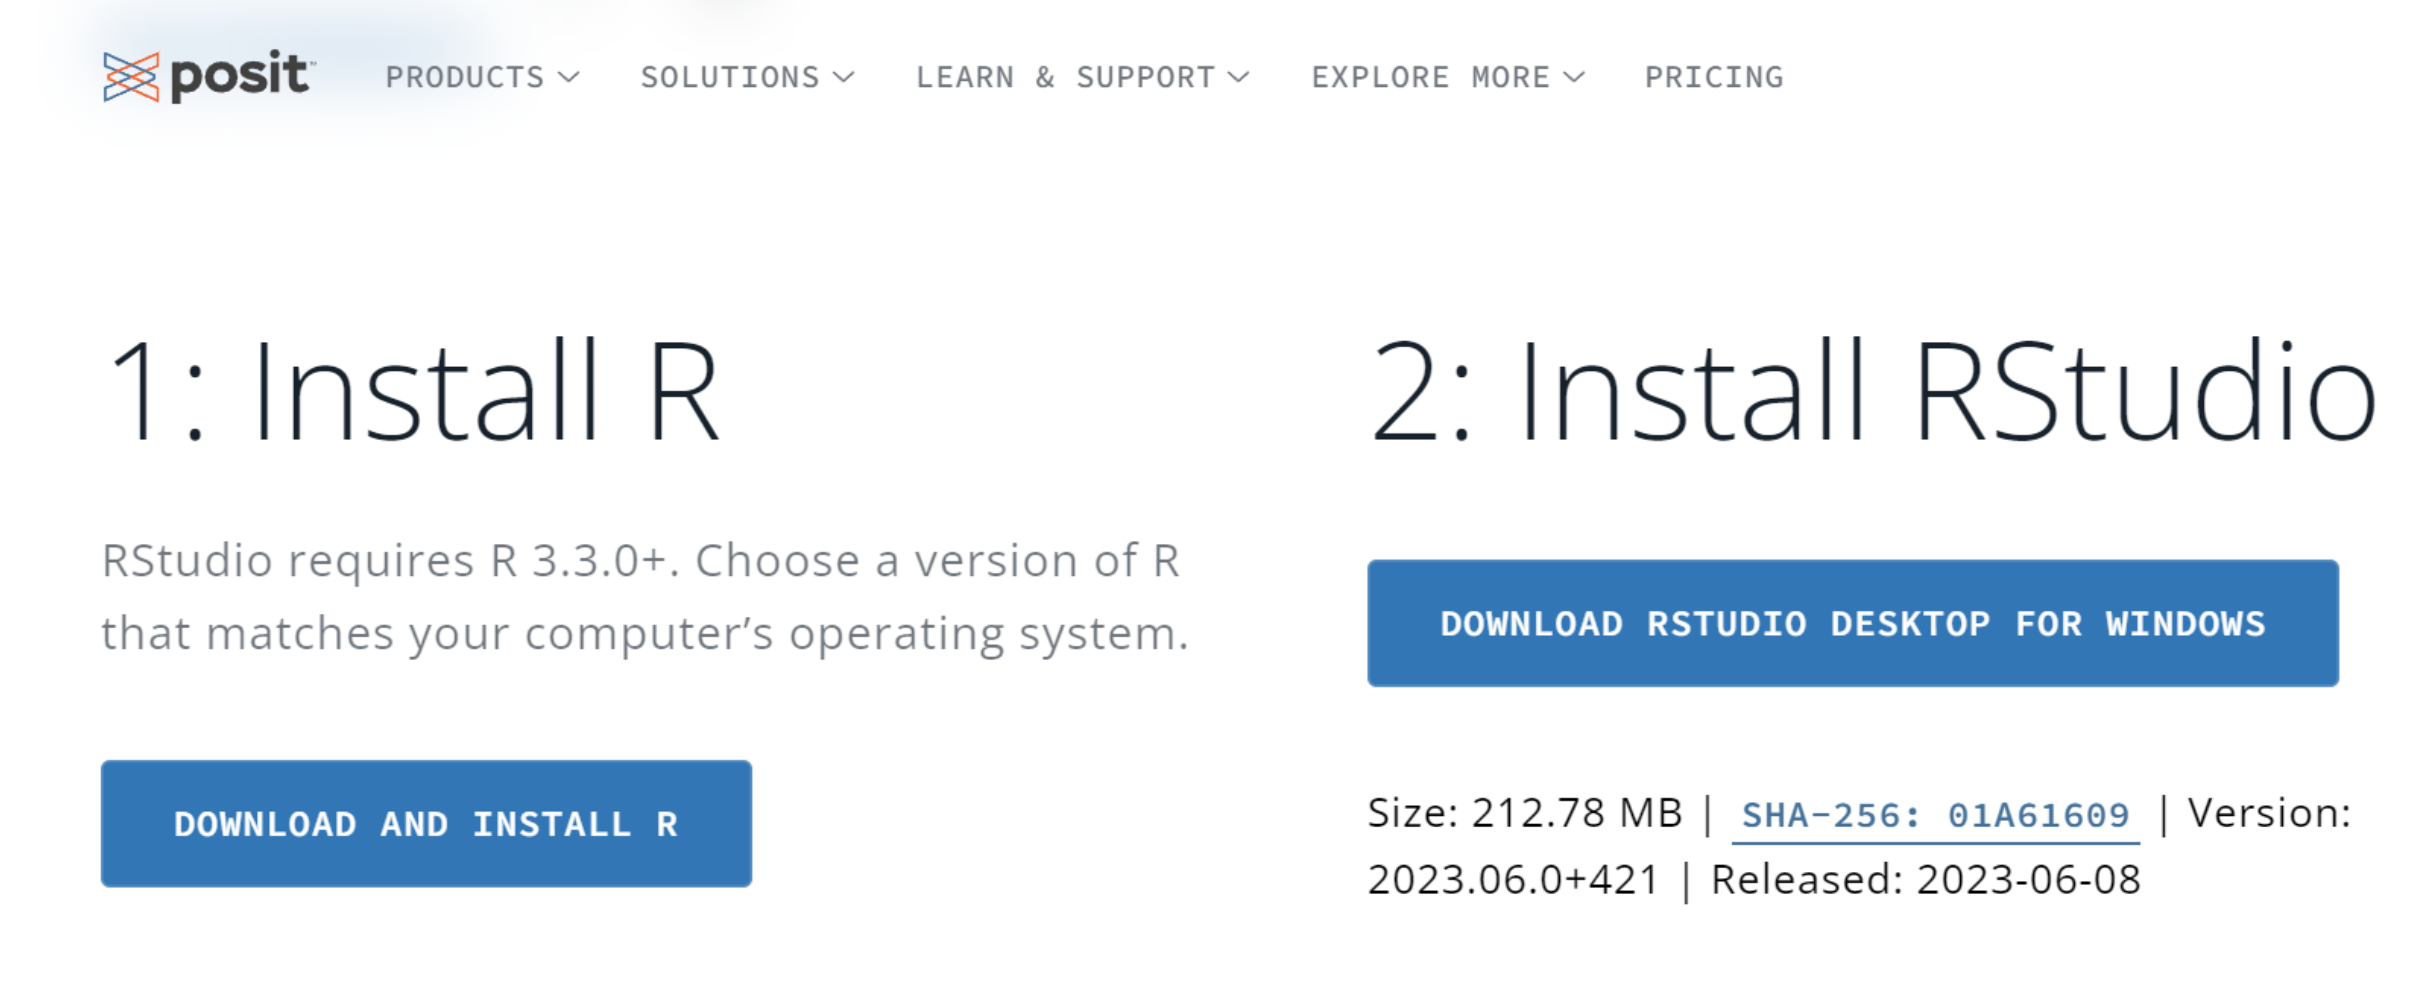
\includegraphics[width=1\linewidth]{./images/posit} 

}

\caption{Instalación de R y RStudio.}\label{fig:posit}
\end{figure}

\hypertarget{rstudio}{%
\section{RStudio}\label{rstudio}}

La primera vez que abrimos RStudio la interfaz nos muestra tres paneles:

\begin{itemize}
\tightlist
\item
  \emph{Panel izquierdo} -\textbf{Consola}: donde corremos el código
\item
  \emph{Panel derecho superior} -solapa \textbf{Entorno}: vemos los datos y funciones que cargamos en la sesión de R.
\item
  \emph{Panel derecho inferior} -solapa \textbf{Files}: directorio de trabajo y archivos dentro de la carpeta.
\item
  \emph{Panel derecho inferior} -solapa: \textbf{Gráficos}: visualización de plots.
\item
  \emph{Panel derecho inferior} -solapa: \textbf{Paquetes}: visualización/carga/actualización de paquetes de R.
\item
  \emph{Panel derecho inferior} -solapa: \textbf{Ayuda}: Recuerde que puede buscar ayuda desde esta solapa o tipeado en la consola \texttt{?nombre\_del\_comando}.
\end{itemize}

\begin{figure}

{\centering 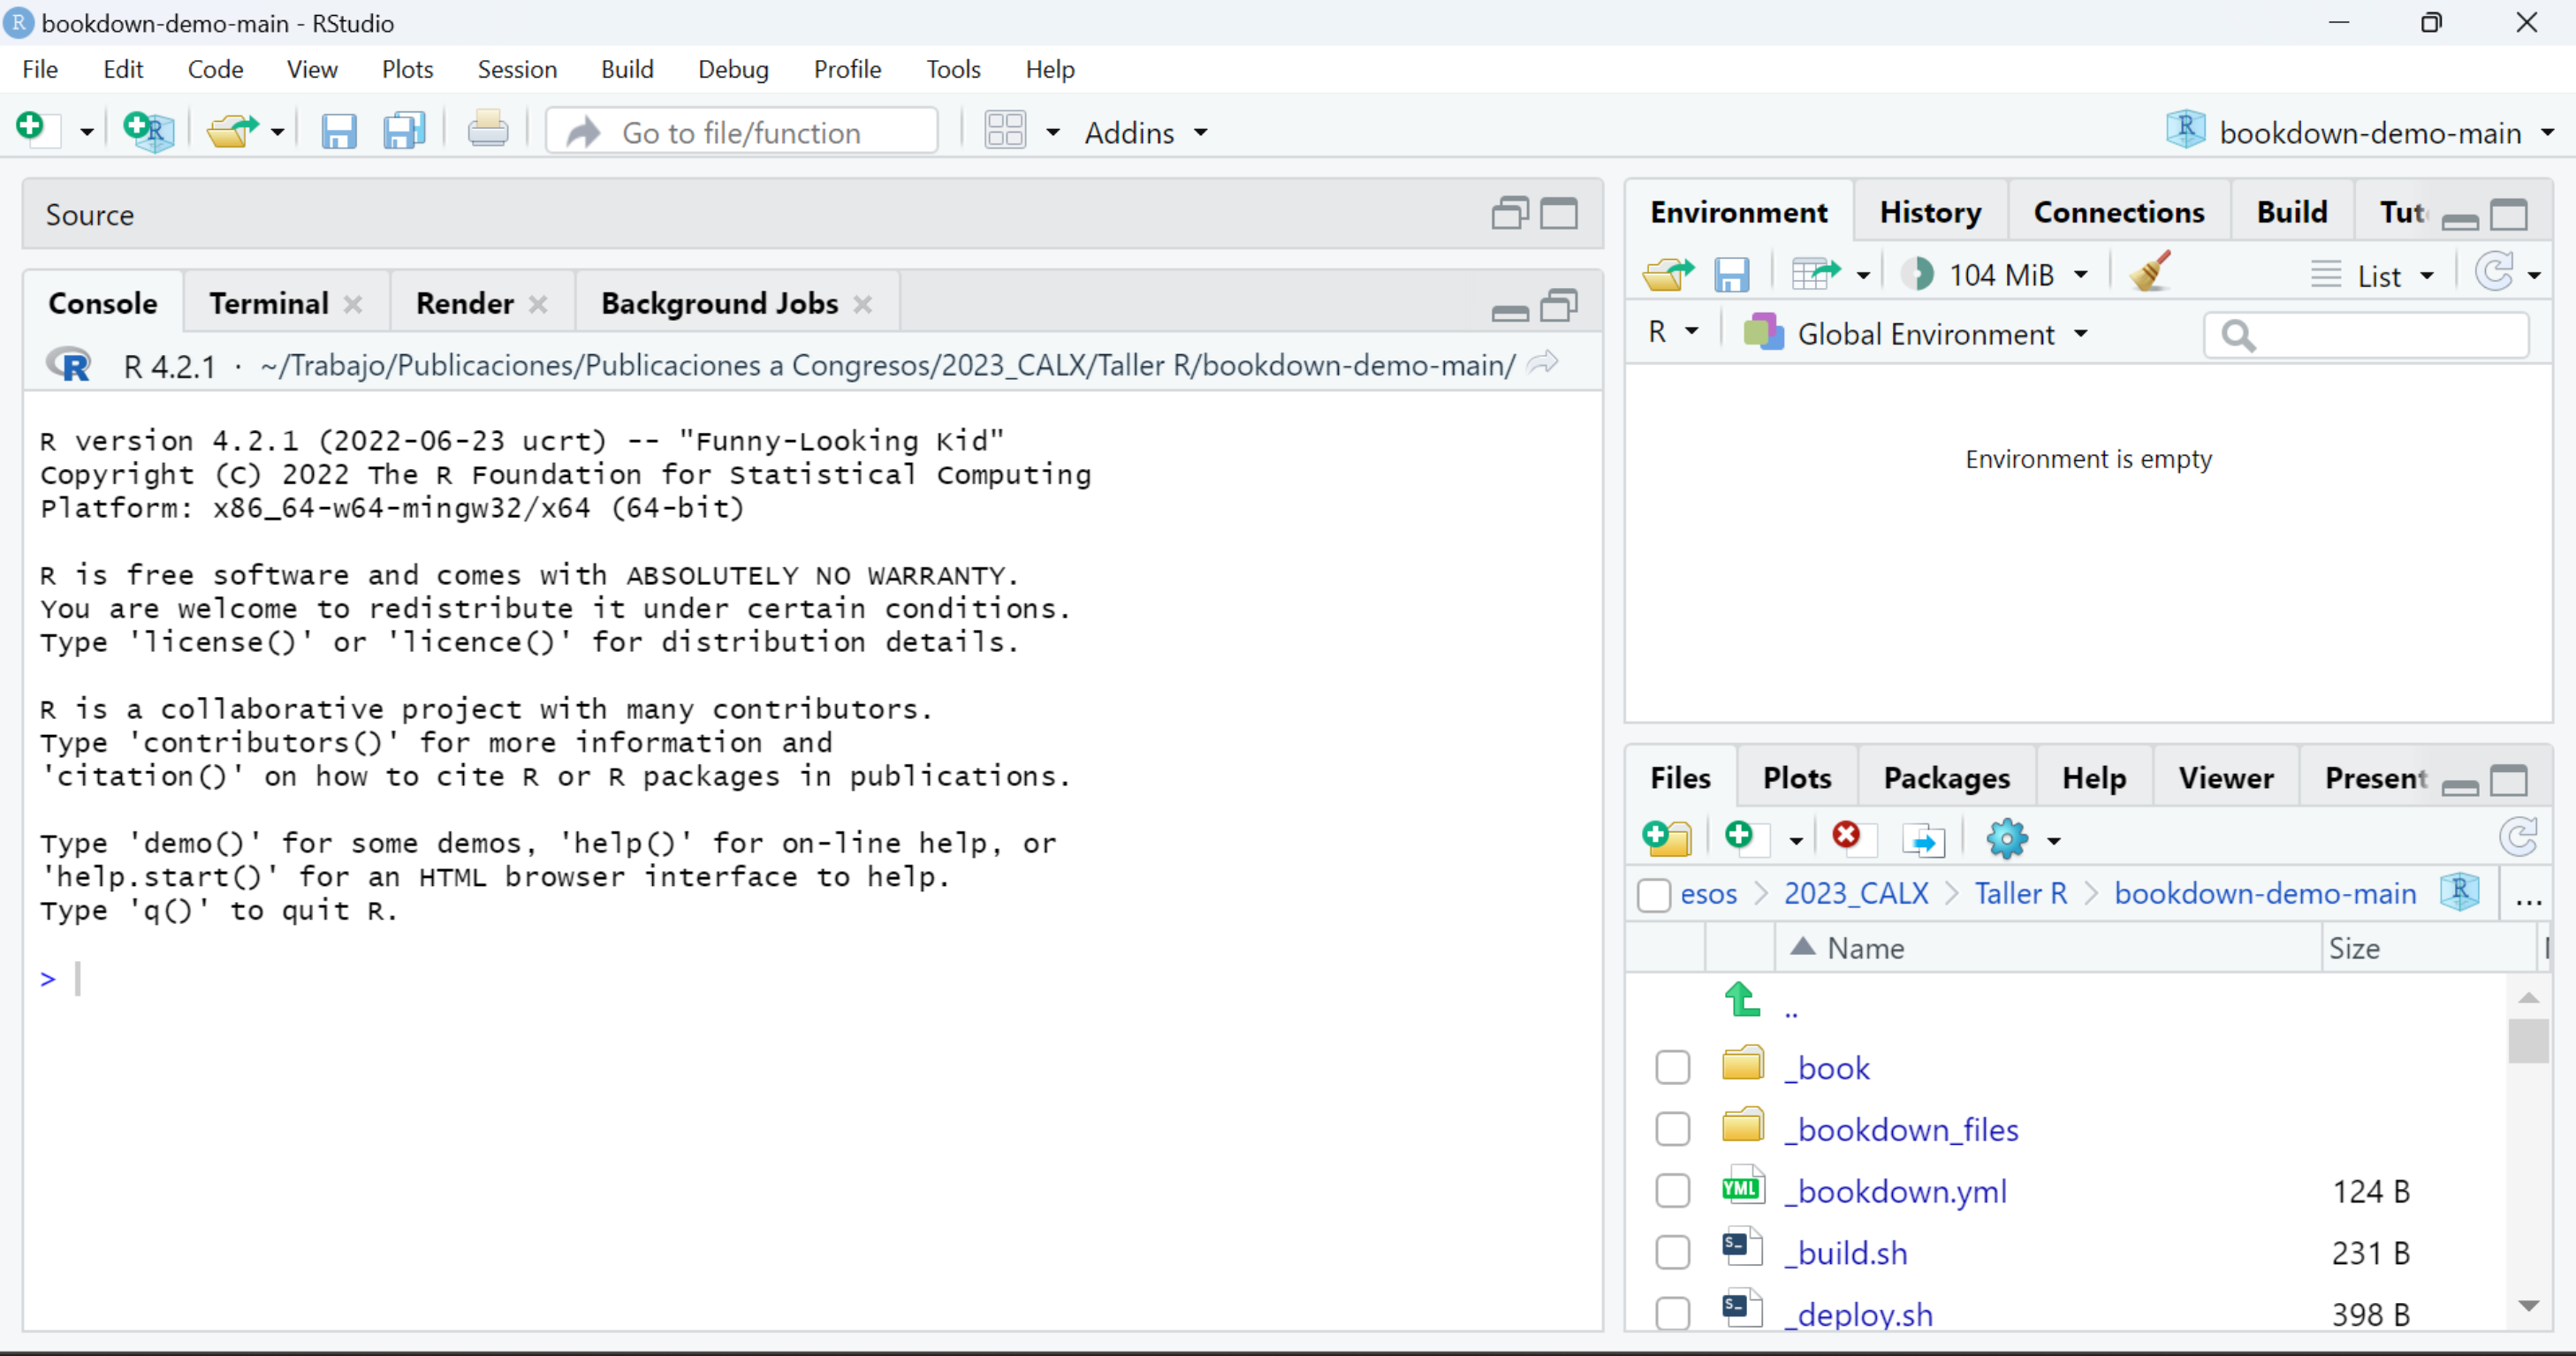
\includegraphics[width=1\linewidth]{./images/rstudio} 

}

\caption{Interfaz de RStudio.}\label{fig:rstudio}
\end{figure}

\hypertarget{a-trabajar}{%
\section{A trabajar!}\label{a-trabajar}}

\hypertarget{crear-un-proyecto}{%
\subsection{\texorpdfstring{Crear un \textbf{Proyecto}}{Crear un Proyecto}}\label{crear-un-proyecto}}

\begin{enumerate}
\def\labelenumi{\arabic{enumi}.}
\tightlist
\item
  Click en \texttt{File} ( \emph{esquina superior izquierda en} Figura \ref{fig:rstudio}).
\item
  Click en \texttt{New\ Project}.
\item
  Click en \texttt{New\ Directory}.
\item
  Click en \texttt{New\ Project}.
\item
  Escribir el nombre de la carpeta, que será el \textbf{Directorio de Trabajo} y contendrá el \textbf{Proyecto}. Se puede setear la ubicación de la carpeta haciendo click en \texttt{Browse}. En la Figura \ref{fig:project} se creó la carpeta LimonologiaR\_U01 en el Escritorio.
\item
  Click en \texttt{Create\ Project}.
\end{enumerate}

\begin{figure}

{\centering 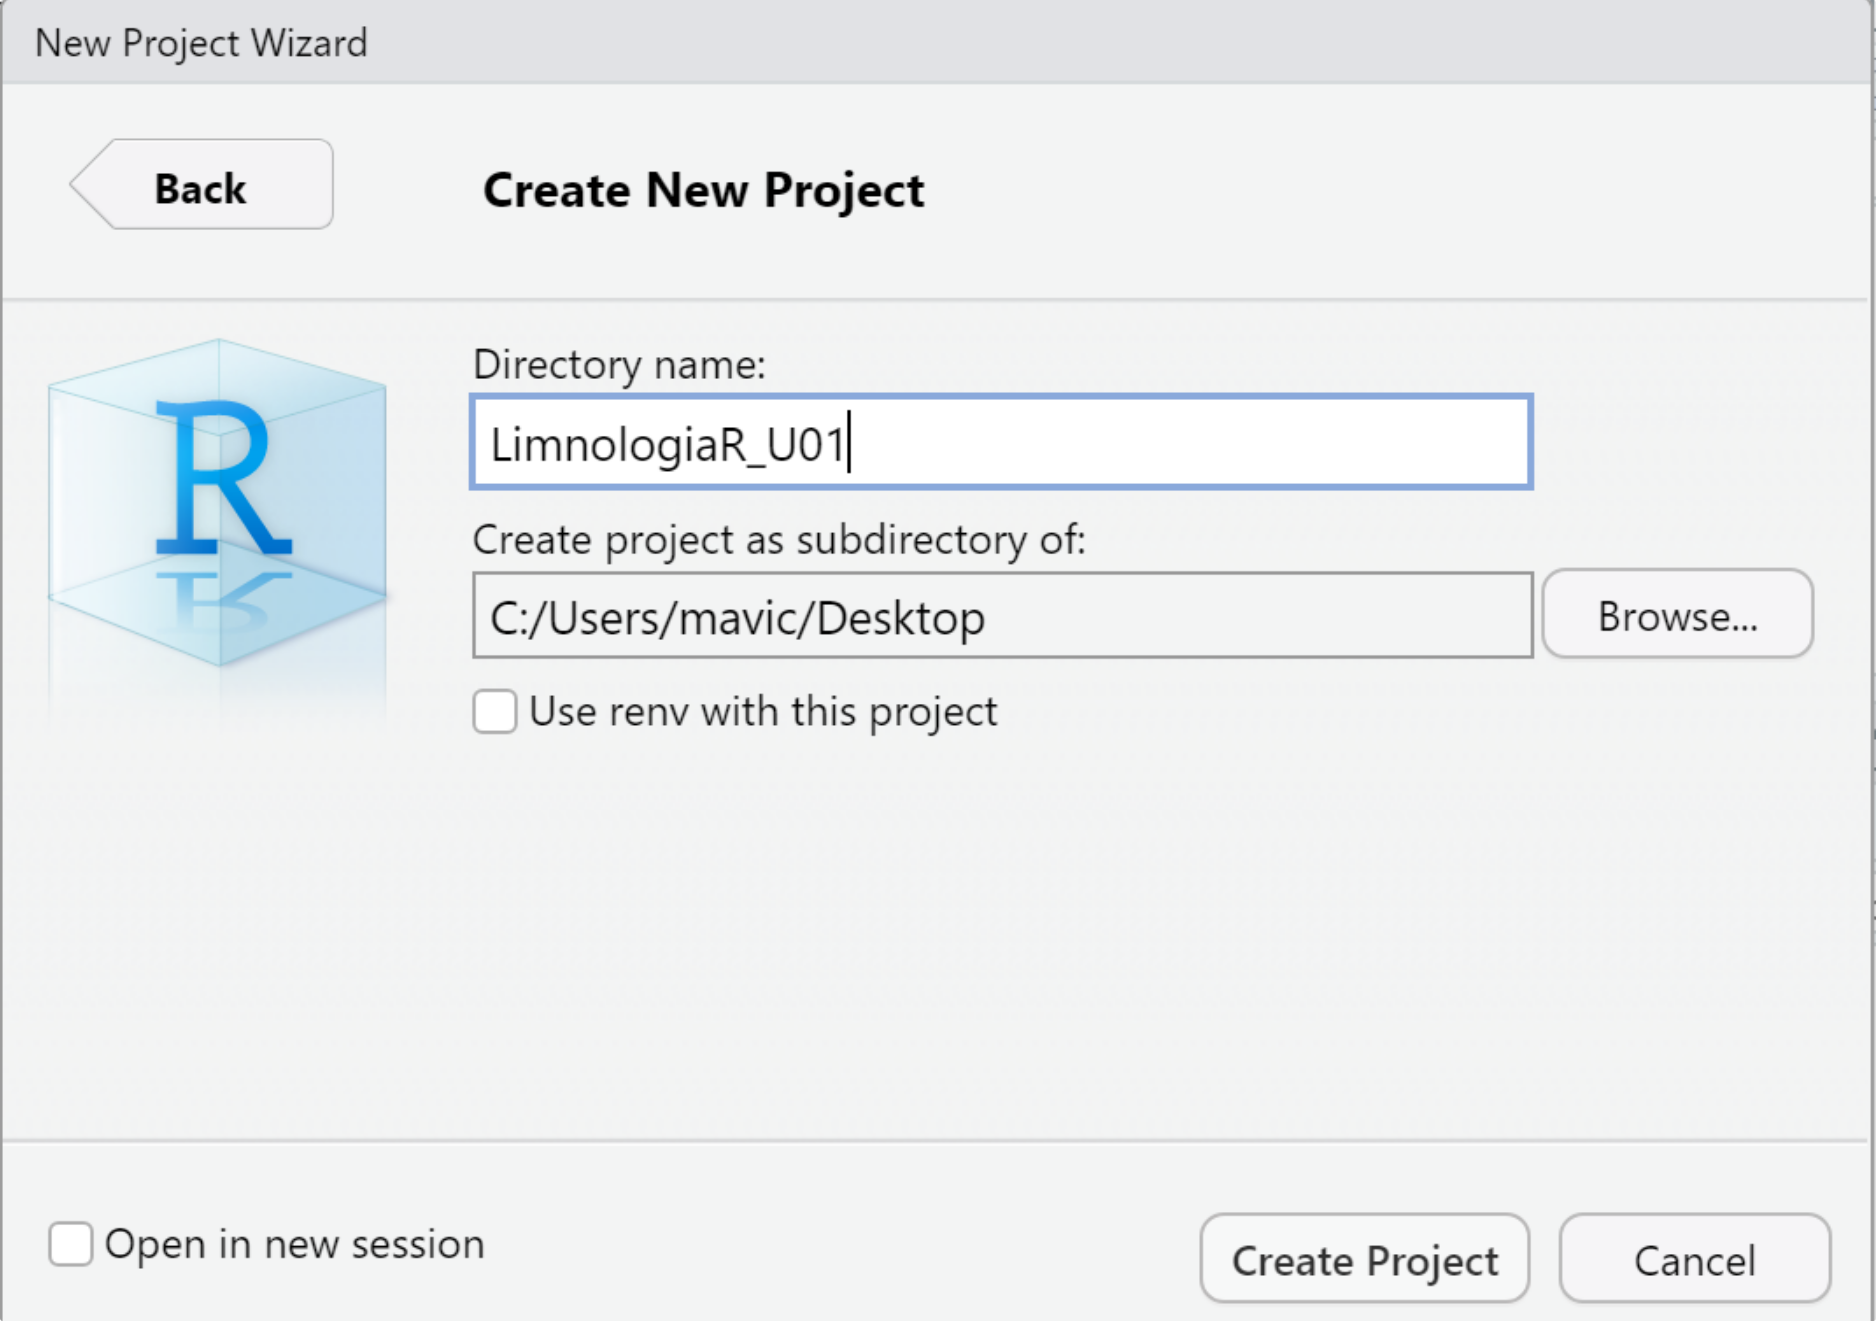
\includegraphics[width=0.75\linewidth]{./images/project} 

}

\caption{Crear un nuevo proyecto para la Unidad 1.}\label{fig:project}
\end{figure}

Ver el \textbf{Directorio de Trabajo}:

\begin{Shaded}
\begin{Highlighting}[]
\FunctionTok{getwd}\NormalTok{()}
\end{Highlighting}
\end{Shaded}

\emph{Recomendaciones:}

Crear una carpeta para cada unidad, para tener los análisis separados y ordenados.

Generar nombres de carpetas y archivos \textbf{sin} espacios, acentos o caracteres especiales.

\hypertarget{crear-un-r-script}{%
\subsection{\texorpdfstring{Crear un \textbf{R Script}}{Crear un R Script}}\label{crear-un-r-script}}

\begin{enumerate}
\def\labelenumi{\arabic{enumi}.}
\tightlist
\item
  Click en \texttt{New\ file}.
\item
  Click en \texttt{R\ Script}.
\end{enumerate}

\begin{itemize}
\tightlist
\item
  Se puede utilizar el atajo \texttt{Ctrl+Shift+N}.
\end{itemize}

Recuerde las recomendaciones para nombrar archivos al \texttt{guardar} el script.

El script se va a guardar como archivo \emph{.R} en el \textbf{Directorio de Trabajo}.

\begin{figure}

{\centering 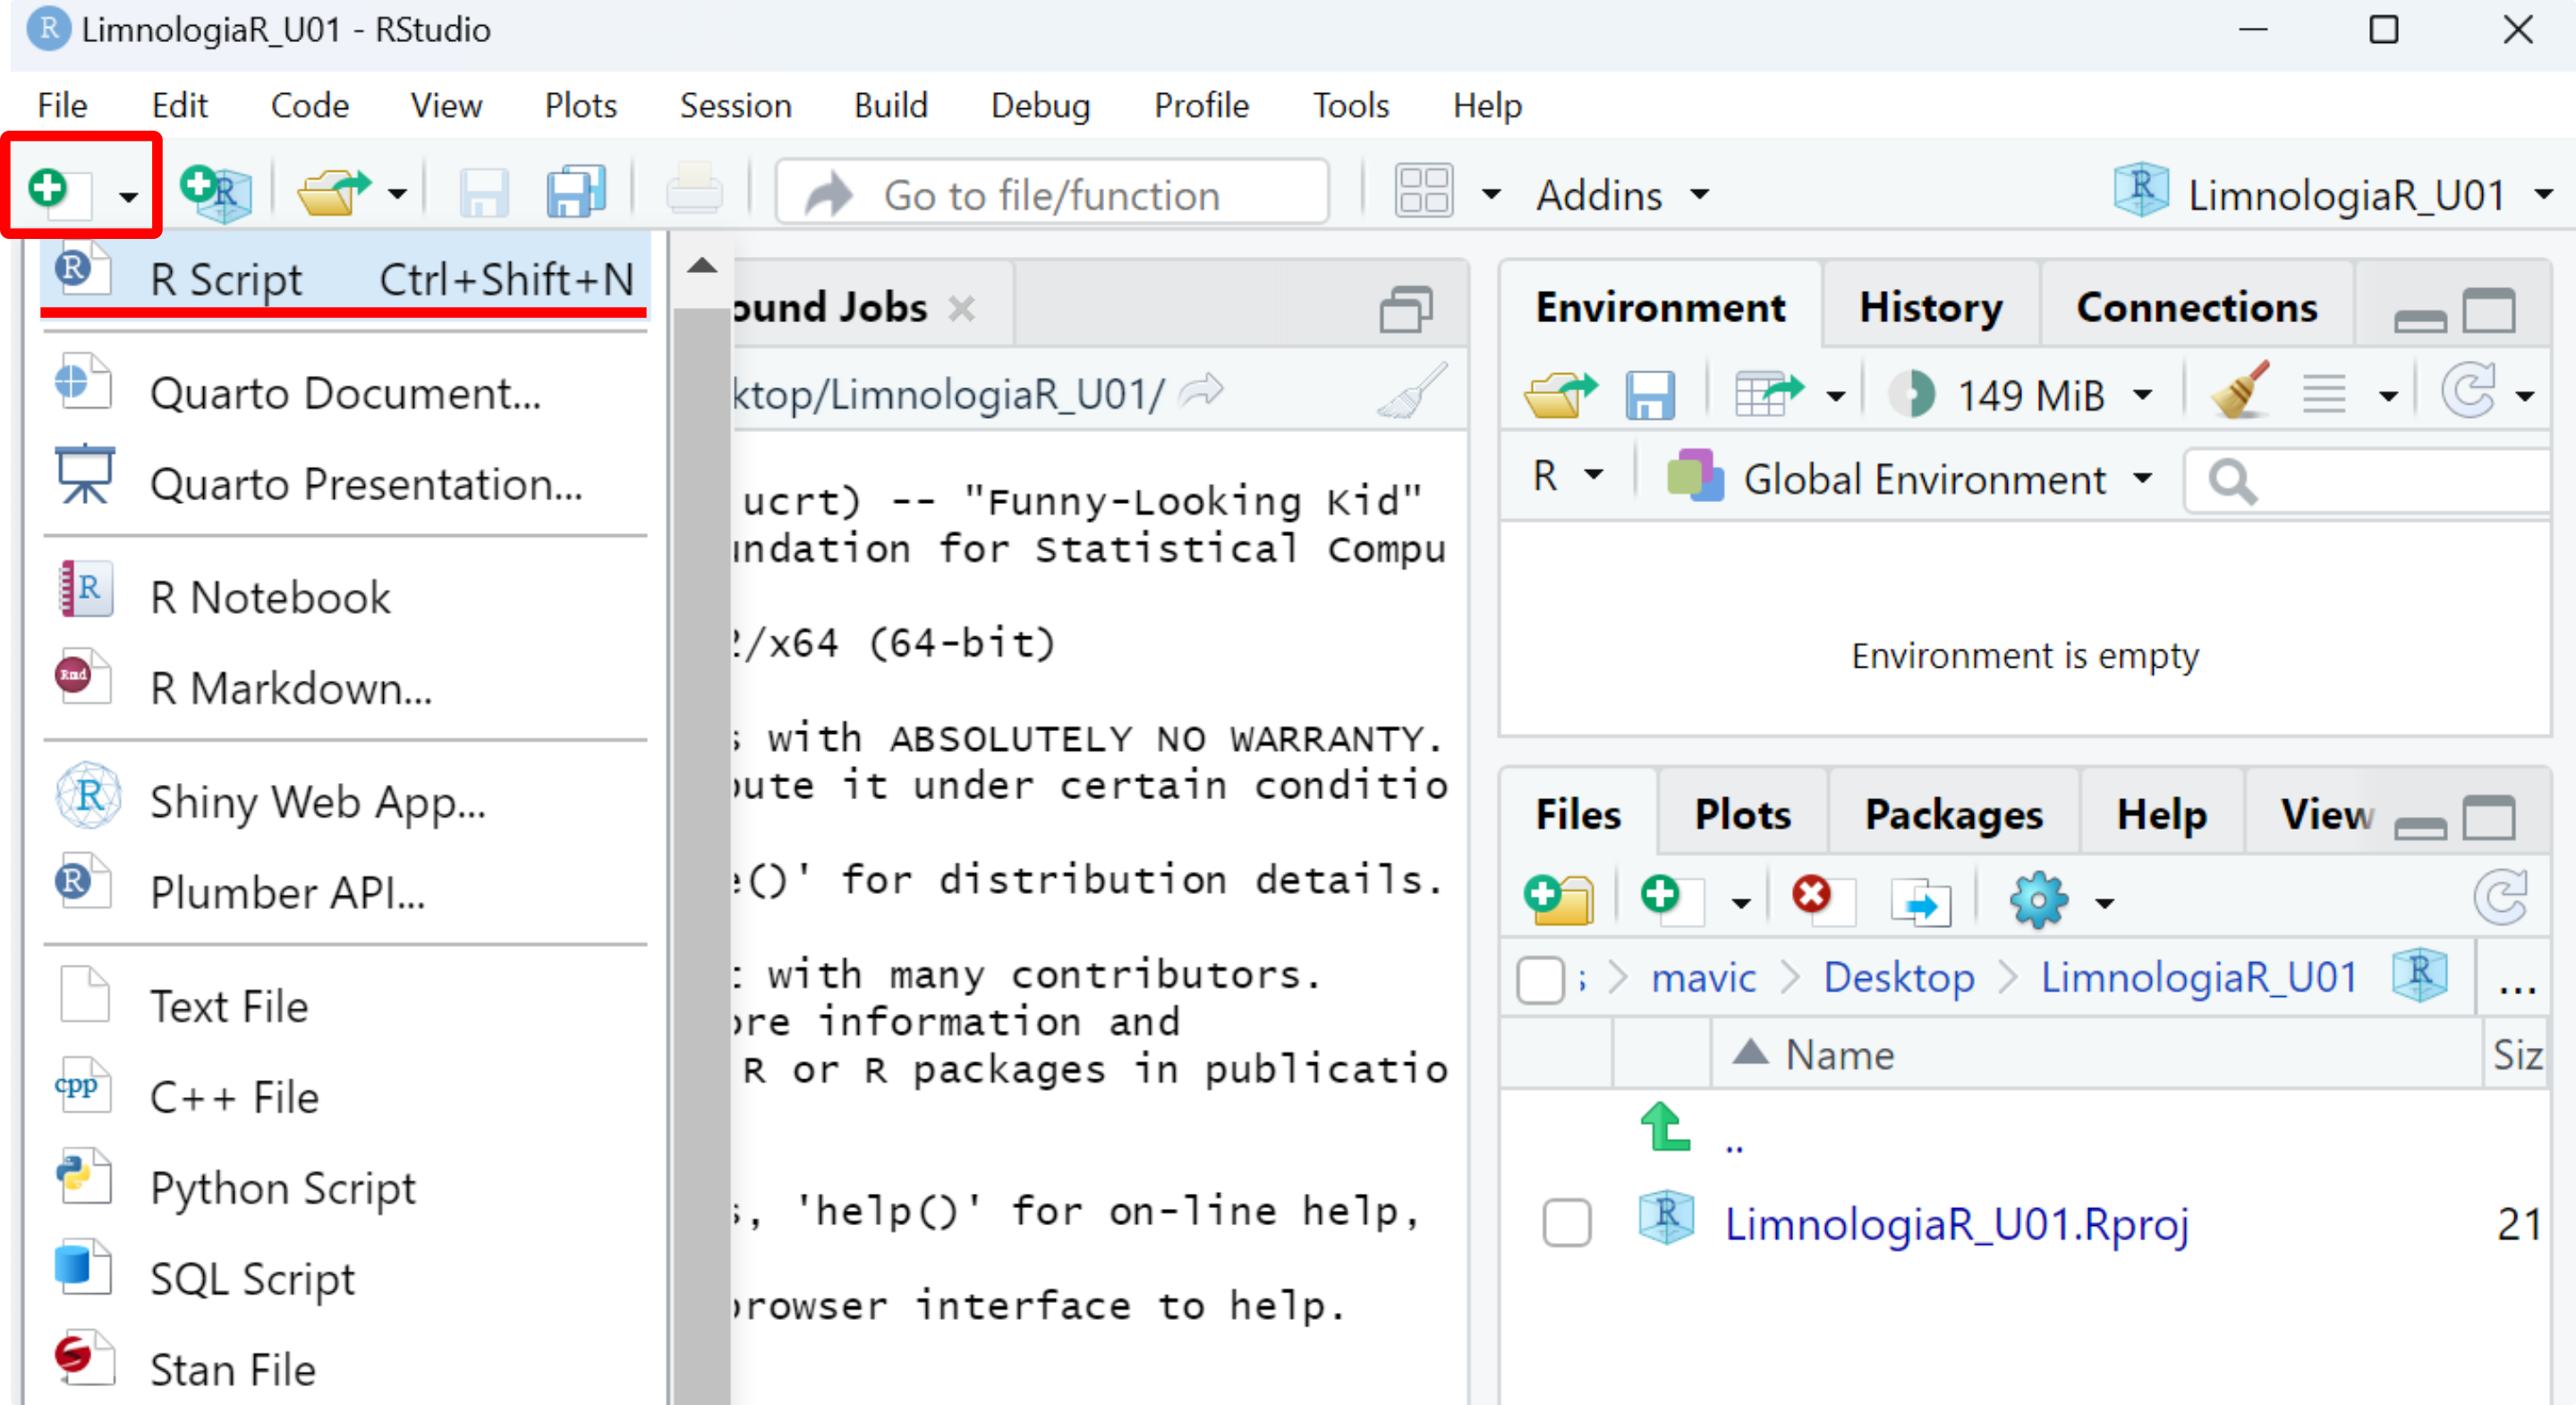
\includegraphics[width=0.75\linewidth]{./images/script} 

}

\caption{Crear un nuevo R Script.}\label{fig:script}
\end{figure}

En este \textbf{script} se escribe y guarda el código.

Una forma fácil de copiar código es utilizando el botón \texttt{Copy\ to\ clipboard} que se encuentra en la esquina superior izquierda de los \texttt{bloques\ de\ código} (Figura \ref{fig:copycode}).

\begin{figure}

{\centering 
\includegraphics[width=0.3\linewidth]{./images/copycode} 

}

\caption{Copiar código desde el material del taller.}\label{fig:copycode}
\end{figure}

Se pega o escribe \texttt{código} en el \textbf{script} y se \texttt{guarda} haciendo click como se indica en el \emph{recuadro 1} de la Figura \ref{fig:code}.

El código en el \textbf{script} se \texttt{ejecuta} haciendo click en \texttt{Run\ the\ current\ line\ or\ selection} ( \emph{recuadro 2} en Figura \ref{fig:code}). Podemos ejecutar de una línea por vez: nos situamos en una línea y hacemos click; o podemos ejecutar varias líneas juntas: seleccionamos el set de líneas y hacemos click. La última opción \emph{no} se recomineda si es la primera vez que corre el código.

El código se ejecuta en la \textbf{consola} Figura \ref{fig:code}.\textbf{2}.

Se observan los resultados en la \textbf{consola} Figura \ref{fig:code}.\textbf{3}.

Los resultados se pueden copiar de la \textbf{consola} y pegar en el \textbf{script}. Recuerde marcar los resultados como comentarios (líneas que comienzan con \texttt{\#}). \emph{Atajo: seleccionar todas las lineas de resultados y presionar} \texttt{Ctrl+Shift+C}.

R \textbf{no} ejecuta lo que se encuentra después de \texttt{\#}.

\begin{figure}

{\centering 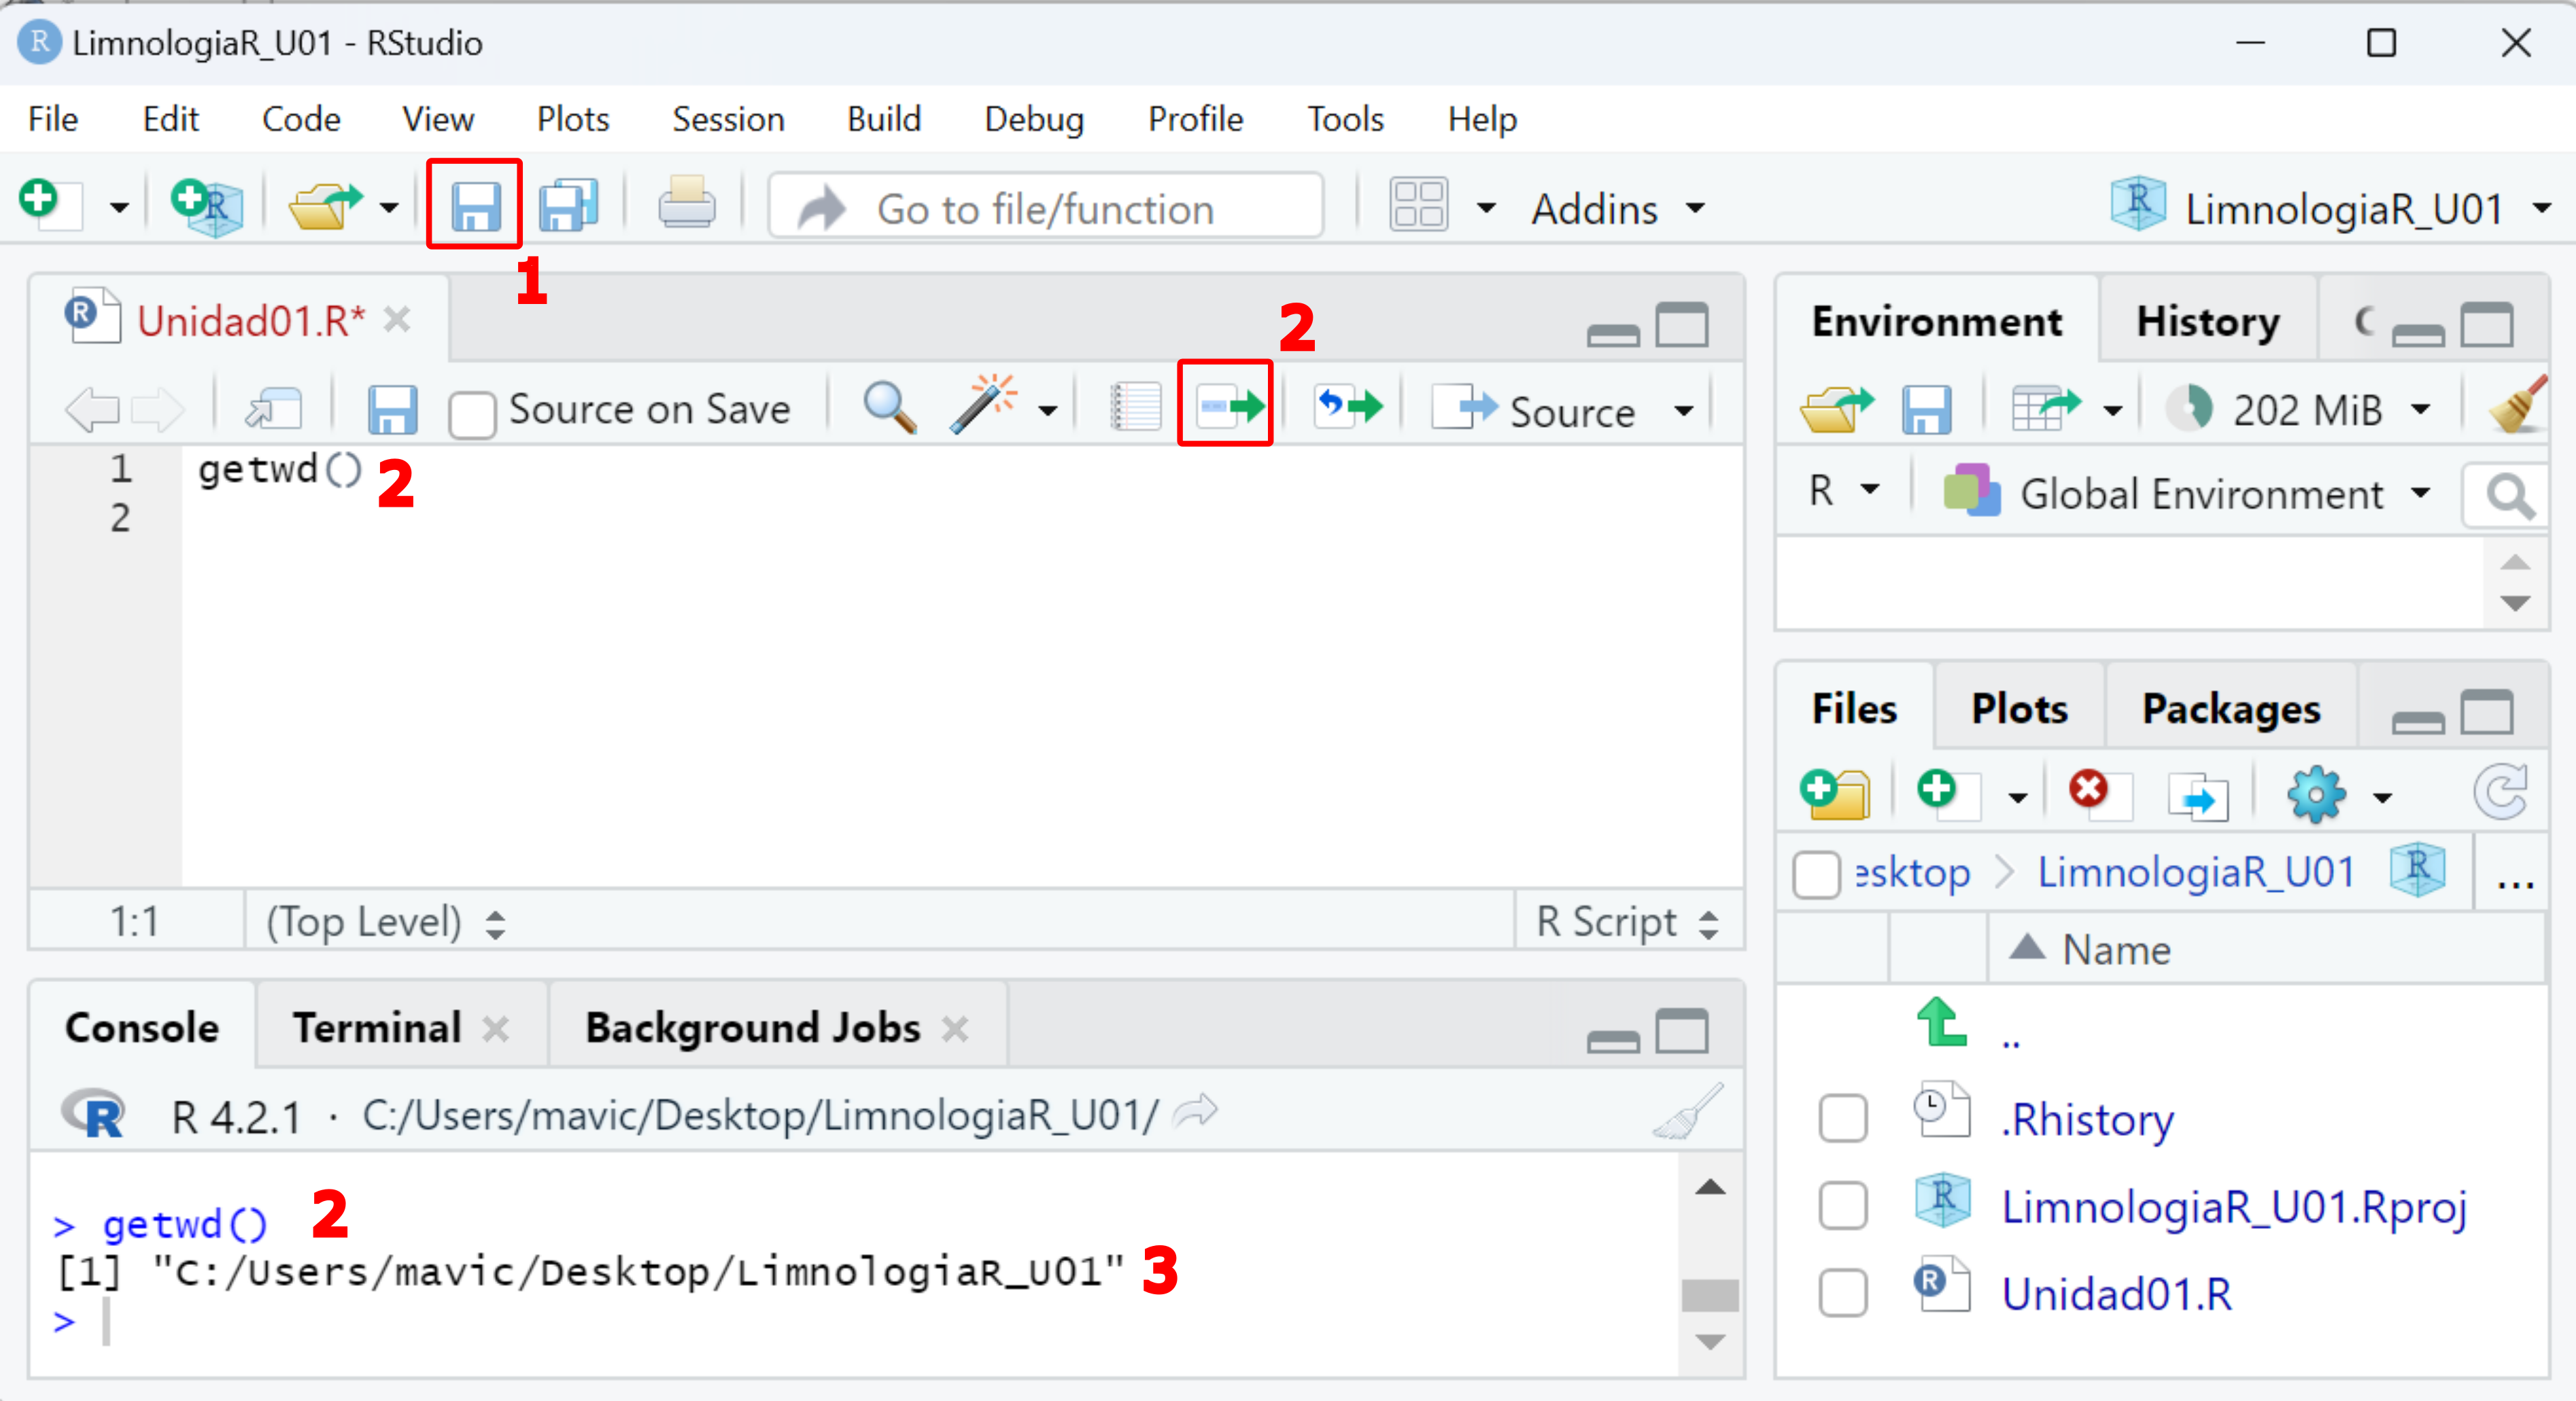
\includegraphics[width=1\linewidth]{./images/code} 

}

\caption{Trabajo en la interfaz de RStudio. 1- Guardar Script. 2- Ejecutar código desde Script. 3- Resultados en consola}\label{fig:code}
\end{figure}

\hypertarget{instalar-y-cargar-paquetes}{%
\subsection{\texorpdfstring{Instalar y cargar \textbf{paquetes}}{Instalar y cargar paquetes}}\label{instalar-y-cargar-paquetes}}

Los paquetes se instalan (por única vez) desde la \textbf{consola} con \texttt{install.packages("nombre")} o desde la interfase de la solapa \textbf{Packages}.

Los paquetes se cargan en la sesión con \texttt{library("nombre")}.

\begin{itemize}
\tightlist
\item
  \textbf{Buenas prácticas!} Conviene poner todas las librerías que se vayan a usar al comienzo.
\end{itemize}

\hypertarget{importar-datos}{%
\subsection{\texorpdfstring{Importar \textbf{datos}}{Importar datos}}\label{importar-datos}}

Hay diversas maneras de leer datos. Podemos leer datos

\begin{itemize}
\item
  \emph{.txt}

  \begin{itemize}
  \tightlist
  \item
    Conviene guardar la base de datos como txt (Tab delimited); donde las columnas quedan definidas por espacios.
  \end{itemize}
\item
  \emph{.csv} Comma/Separated Values

  \begin{itemize}
  \tightlist
  \item
    Archivos de texto separados por comas. Se forma una tabla de filas y columnas
  \end{itemize}
\item
  \emph{.xls}
\end{itemize}

Generalmente se utiliza un comando \texttt{read}, por ejemplo \texttt{read.csv("Nombre\ del\ archivo.csv")}, según el tipo de archivo que se trate (txt, xlsx, etc.)

Una vez que tenemos cargado nuestro conjunto de datos nos puede interesar realizar algunos comandos exploratorios que nos van a dar información acerca de este \emph{data frame} (estructura de datos).

\begin{itemize}
\tightlist
\item
  \texttt{summary(objeto)}

  \begin{itemize}
  \tightlist
  \item
    La salida va a depender de la clase de objeto al cual lo aplicamos.
  \item
    Útil para ver información básica sobre nuestras variables
  \item
    Para \emph{data frames} el summary nos devuelve el valor mínimo, máximo, la mediana y el 1er y 3er cuantil.
  \item
    Si se aplica para salidas de modelos lineales (Ver Unidad 2), nos proporciona información acerca de los residuos, los coeficientes del modelo, el error estándar residual, R\textsuperscript{2}, el R ajustado, el estadístico F y el p valor.
  \end{itemize}
\item
  \texttt{str(objeto)}

  \begin{itemize}
  \tightlist
  \item
    Nos devuelve cuántas observaciones tiene el data frame, información acerca de las variables (son numéricas? factores?); como esta estructurado nuestro conjunto de datos.
  \end{itemize}
\item
  \texttt{head(objeto)} y \texttt{tail(objeto)}

  \begin{itemize}
  \tightlist
  \item
    Nos da las primeras y últimas filas, respectivamente.
  \end{itemize}
\item
  \texttt{class(objeto)}

  \begin{itemize}
  \tightlist
  \item
    Devuelve qué tipo de objeto es (data frame, matrix, vector, etc).
  \end{itemize}
\end{itemize}

\begin{Shaded}
\begin{Highlighting}[]
\FunctionTok{data}\NormalTok{(}\StringTok{"iris"}\NormalTok{)}

\FunctionTok{summary}\NormalTok{(iris)}
\end{Highlighting}
\end{Shaded}

\begin{verbatim}
##   Sepal.Length    Sepal.Width     Petal.Length    Petal.Width   
##  Min.   :4.300   Min.   :2.000   Min.   :1.000   Min.   :0.100  
##  1st Qu.:5.100   1st Qu.:2.800   1st Qu.:1.600   1st Qu.:0.300  
##  Median :5.800   Median :3.000   Median :4.350   Median :1.300  
##  Mean   :5.843   Mean   :3.057   Mean   :3.758   Mean   :1.199  
##  3rd Qu.:6.400   3rd Qu.:3.300   3rd Qu.:5.100   3rd Qu.:1.800  
##  Max.   :7.900   Max.   :4.400   Max.   :6.900   Max.   :2.500  
##        Species  
##  setosa    :50  
##  versicolor:50  
##  virginica :50  
##                 
##                 
## 
\end{verbatim}

\begin{Shaded}
\begin{Highlighting}[]
\FunctionTok{str}\NormalTok{(iris)}
\end{Highlighting}
\end{Shaded}

\begin{verbatim}
## 'data.frame':    150 obs. of  5 variables:
##  $ Sepal.Length: num  5.1 4.9 4.7 4.6 5 5.4 4.6 5 4.4 4.9 ...
##  $ Sepal.Width : num  3.5 3 3.2 3.1 3.6 3.9 3.4 3.4 2.9 3.1 ...
##  $ Petal.Length: num  1.4 1.4 1.3 1.5 1.4 1.7 1.4 1.5 1.4 1.5 ...
##  $ Petal.Width : num  0.2 0.2 0.2 0.2 0.2 0.4 0.3 0.2 0.2 0.1 ...
##  $ Species     : Factor w/ 3 levels "setosa","versicolor",..: 1 1 1 1 1 1 1 1 1 1 ...
\end{verbatim}

\begin{Shaded}
\begin{Highlighting}[]
\FunctionTok{head}\NormalTok{(iris)}
\end{Highlighting}
\end{Shaded}

\begin{verbatim}
##   Sepal.Length Sepal.Width Petal.Length Petal.Width Species
## 1          5.1         3.5          1.4         0.2  setosa
## 2          4.9         3.0          1.4         0.2  setosa
## 3          4.7         3.2          1.3         0.2  setosa
## 4          4.6         3.1          1.5         0.2  setosa
## 5          5.0         3.6          1.4         0.2  setosa
## 6          5.4         3.9          1.7         0.4  setosa
\end{verbatim}

\begin{Shaded}
\begin{Highlighting}[]
\FunctionTok{class}\NormalTok{(iris)}
\end{Highlighting}
\end{Shaded}

\begin{verbatim}
## [1] "data.frame"
\end{verbatim}

\hypertarget{visualizar-y-manipular-datos}{%
\subsection{\texorpdfstring{Visualizar y manipular \textbf{datos}}{Visualizar y manipular datos}}\label{visualizar-y-manipular-datos}}

Qué tipo de variables hay?

Existen variables numéricas (num), factores (que pueden tener varios niveles, factor), char o de caracter. Generalmente R detecta el tipo de variable al cargar los datos. Se puede transformar variables entre sí.

\begin{itemize}
\tightlist
\item
  \textbf{Observación} El comando \texttt{c()} nos permite concatenar elementos. Siempre que se selecciona más de un elemento se debe concatenar.
\end{itemize}

Por ejemplo,

\begin{Shaded}
\begin{Highlighting}[]
\NormalTok{variable }\OtherTok{\textless{}{-}} \FunctionTok{c}\NormalTok{(}\DecValTok{1}\NormalTok{,}\DecValTok{2}\NormalTok{,}\DecValTok{1}\NormalTok{,}\DecValTok{1}\NormalTok{,}\DecValTok{1}\NormalTok{,}\DecValTok{2}\NormalTok{,}\DecValTok{2}\NormalTok{,}\DecValTok{2}\NormalTok{,}\DecValTok{1}\NormalTok{)}

\FunctionTok{class}\NormalTok{(variable)}
\end{Highlighting}
\end{Shaded}

\begin{verbatim}
## [1] "numeric"
\end{verbatim}

\begin{Shaded}
\begin{Highlighting}[]
\NormalTok{factor }\OtherTok{\textless{}{-}} \FunctionTok{factor}\NormalTok{(variable, }\AttributeTok{levels =} \FunctionTok{c}\NormalTok{(}\DecValTok{1}\NormalTok{,}\DecValTok{2}\NormalTok{), }\AttributeTok{labels=}\FunctionTok{c}\NormalTok{(}\StringTok{"Nivel 1"}\NormalTok{, }\StringTok{"Nivel 2"}\NormalTok{))}
\end{Highlighting}
\end{Shaded}

De esta manera, transformamos una variable numerica en un factor con dos niveles, Nivel 1 y 2. Nos puede ser útil en caso de tener una variable tomada desde campo (o de encuestas) como numérica y querramos que sea categórica.

Podemos acceder a elementos particulares dentro del data frame, ya sea porque nos interesa ver ese elemento individual, para sacarlo del data frame, \textbf{para armar filtros} o para realizar ciertos análisis con una parte del data frame. Se trabaja con coordenadas (x,y), donde \textbf{x} es la fila e \textbf{y} la columna.

Si quiero todos los datos de una fila en particular, por ejemplo la 17 se escribe \texttt{iris{[}17,{]}} (seleccionamos la fila y las columnas quedan vacías porque queremos verlas todas).

De la misma manera, si queremos ver solamente una columna \texttt{iris{[},3{]}}. También podemos llamarlo según el nombre de la misma \texttt{iris{[},"Species"{]}}.

Para seleccionar los primeros 10 datos \texttt{iris{[}1:10,{]}} (o con el comando que ya vimos \textbf{Head()}).

Si queremos seleccionar \textbf{varias filas} simplemente las concatenamos. Entonces si escribimos\texttt{iris{[}c(1:5),\ c(2,3){]}} Qué seleccionamos en este caso?

Qué pasa si quiero seleccionar una sola variable? Podemos! El signo \textbf{\$} indica que se selecciona una columna dentro del dataframe que lo precede.

\texttt{iris\$Sepcies} me permite ver toda la columna de la variable Especies. De esta manera, incluso podemos crear variables nuevas, asignandolas de la siguiente manera

\begin{Shaded}
\begin{Highlighting}[]
\NormalTok{iris}\SpecialCharTok{$}\NormalTok{variable.nueva }\OtherTok{\textless{}{-}}\NormalTok{ iris}\SpecialCharTok{$}\NormalTok{Sepal.Length}\SpecialCharTok{/}\NormalTok{iris}\SpecialCharTok{$}\NormalTok{Sepal.Width}
\end{Highlighting}
\end{Shaded}

Qué variable nueva acabamos de crear?

\begin{itemize}
\tightlist
\item
  \textbf{Ojo!} Si no le asignamos el dataframe a la variable nueva con el signo \texttt{\$} (\texttt{iris\$variablenueva}) el R la va a crear por fuera de nuesto data frame como un vector de los valores.
\end{itemize}

\uline{Subsets}

Como lo indica el nombre, nos quedamos con una porción que seleccionemos del data frame, y sobre el cual podremos operar de manera independiente, sin que el data frame original se vea afectado.

En el ejemplo con iris, podemos crear un subset que contenga solamente a la especie iris setosa.

\begin{Shaded}
\begin{Highlighting}[]
\NormalTok{setosa }\OtherTok{\textless{}{-}} \FunctionTok{subset}\NormalTok{(iris, iris}\SpecialCharTok{$}\NormalTok{Species}\SpecialCharTok{==}\StringTok{"setosa"}\NormalTok{)}
\end{Highlighting}
\end{Shaded}

Para aquellos que se sientan más cómodos, la libreria \textbf{dplyr} permite hacer que las selecciones y filtros sea más fácil. Suma mucho a la facilidad del trabajo aprender a usarla!

\begin{Shaded}
\begin{Highlighting}[]
\FunctionTok{library}\NormalTok{(dplyr)}

\NormalTok{setosa.dplyr }\OtherTok{\textless{}{-}}\NormalTok{ iris }\SpecialCharTok{\%\textgreater{}\%} 
  \FunctionTok{filter}\NormalTok{ (Species }\SpecialCharTok{\%in\%} \StringTok{"setosa"}\NormalTok{) }
\end{Highlighting}
\end{Shaded}

Hay muchas formas de hacer subsets! Es cuestion de usar aquella con la que se sientan más cómodos.

\hypertarget{gruxe1ficos-exploratorios-buxe1sicos}{%
\subsection{Gráficos exploratorios básicos}\label{gruxe1ficos-exploratorios-buxe1sicos}}

La visualización de datos es un punto clave dentro de cualquier análisis. Los gráficos son útiles para explorar datos, interpretarlos, identificar patrones, detectar outliers y constituyen una de las mejores maneras de comunicar los resultados.

\uline{¿Qué tipos de gráficos existen?}

Hay una enorme diversidad, e incluso se pueden utilizar combinaciones de ellos para aumentar la información comunicada.

\begin{itemize}
\tightlist
\item
  \textbf{Gráfico de barras}

  \begin{itemize}
  \tightlist
  \item
    Muestra una barra para cada categoría de una variable categórica. El alto muestra el valor observado para cada categoría (Fig 1.A)
  \end{itemize}
\item
  \textbf{Gráfico de puntos/dispersión/\emph{scatter plot}}

  \begin{itemize}
  \tightlist
  \item
    Muestra la relación entre dos variables numéricas.
  \end{itemize}
\item
  \textbf{Histograma}

  \begin{itemize}
  \tightlist
  \item
    Aplica para \emph{variables cuantitativas}. Permite ver la distribucion de la variable.
  \end{itemize}
\item
  \textbf{Boxplot}

  \begin{itemize}
  \tightlist
  \item
    Aplica para \emph{variables cuantitativas}. Muestra una serie de medidas de resumnen para dicha variable. Se suele graficar junto a una variable categórica para permitir la comparación entre niveles.
  \end{itemize}
\end{itemize}

\begin{Shaded}
\begin{Highlighting}[]
\FunctionTok{library}\NormalTok{(ggplot2)}
\end{Highlighting}
\end{Shaded}

\begin{verbatim}
## Warning: package 'ggplot2' was built under R version 4.2.2
\end{verbatim}

\begin{Shaded}
\begin{Highlighting}[]
\FunctionTok{library}\NormalTok{(ggpubr)}
\end{Highlighting}
\end{Shaded}

\begin{verbatim}
## Warning: package 'ggpubr' was built under R version 4.2.2
\end{verbatim}

\begin{Shaded}
\begin{Highlighting}[]
\FunctionTok{library}\NormalTok{(grid)}


\NormalTok{barra }\OtherTok{\textless{}{-}}\NormalTok{ iris }\SpecialCharTok{\%\textgreater{}\%} 
  \FunctionTok{group\_by}\NormalTok{(Species) }\SpecialCharTok{\%\textgreater{}\%} 
  \FunctionTok{summarise}\NormalTok{(}\AttributeTok{n=}\FunctionTok{n}\NormalTok{()) }\SpecialCharTok{\%\textgreater{}\%} 
  \FunctionTok{ggplot}\NormalTok{(}\FunctionTok{aes}\NormalTok{(Species,n, }\AttributeTok{fill=}\NormalTok{Species))}\SpecialCharTok{+}
  \FunctionTok{geom\_bar}\NormalTok{(}\AttributeTok{stat=}\StringTok{"identity"}\NormalTok{)}

\NormalTok{scatter }\OtherTok{\textless{}{-}}\NormalTok{ iris }\SpecialCharTok{\%\textgreater{}\%} 
  \FunctionTok{ggplot}\NormalTok{(}\FunctionTok{aes}\NormalTok{(Sepal.Length, Petal.Length, }\AttributeTok{color=}\NormalTok{Species)) }\SpecialCharTok{+}
  \FunctionTok{geom\_point}\NormalTok{()}

\NormalTok{histo }\OtherTok{\textless{}{-}}\NormalTok{ iris }\SpecialCharTok{\%\textgreater{}\%} 
  \FunctionTok{ggplot}\NormalTok{(}\FunctionTok{aes}\NormalTok{(Sepal.Length, }\AttributeTok{fill=}\NormalTok{Species)) }\SpecialCharTok{+}
  \FunctionTok{geom\_histogram}\NormalTok{()}

\NormalTok{box }\OtherTok{\textless{}{-}}\NormalTok{ iris }\SpecialCharTok{\%\textgreater{}\%} 
  \FunctionTok{ggplot}\NormalTok{(}\FunctionTok{aes}\NormalTok{(Species, Petal.Length, }\AttributeTok{fill=}\NormalTok{Species)) }\SpecialCharTok{+}
  \FunctionTok{geom\_boxplot}\NormalTok{()}
\end{Highlighting}
\end{Shaded}

\begin{Shaded}
\begin{Highlighting}[]
\FunctionTok{ggarrange}\NormalTok{(barra,scatter,histo,box, }\AttributeTok{ncol=}\DecValTok{2}\NormalTok{, }\AttributeTok{nrow =} \DecValTok{2}\NormalTok{, }\AttributeTok{widths =} \FunctionTok{c}\NormalTok{(}\FloatTok{0.5}\NormalTok{,}\FloatTok{0.5}\NormalTok{), }\AttributeTok{labels=}\FunctionTok{c}\NormalTok{(}\StringTok{"A"}\NormalTok{, }\StringTok{"B"}\NormalTok{, }\StringTok{"C"}\NormalTok{, }\StringTok{"D"}\NormalTok{))}
\end{Highlighting}
\end{Shaded}

\begin{verbatim}
## `stat_bin()` using `bins = 30`. Pick better value with `binwidth`.
\end{verbatim}

\begin{figure}

{\centering \includegraphics[width=1\linewidth]{01-introSo_files/figure-latex/unnamed-chunk-8-1} 

}

\caption{Tipos de gráficos. A) Gráfico de barras. B) Scatter plot, gráfico de puntos. C) Histograma. D) Boxplot}\label{fig:unnamed-chunk-8}
\end{figure}

\uline{¿R base o Ggplot2?}

La librería en la que se suelen armar los gráficos y que nunca falta en ningún script es \textbf{ggplot2}. Sin embargo, R permite realizar gráficos nativamente sin librerías.

\emph{R base}

Las ventajas de usar R base para graficar es que es su rapidez para visualizar las relaciones entre variables, sin tener que preocuparnos por acordarnos de la sintaxis del script. Sin embargo, ggplot2 ofrece una variedad de combinaciones de customizacion para presentar los datos difícil de equiparar.

El comando básico es \texttt{plot()}entre dos variables. Es decir,

\begin{Shaded}
\begin{Highlighting}[]
\FunctionTok{plot}\NormalTok{(iris}\SpecialCharTok{$}\NormalTok{Petal.Length,iris}\SpecialCharTok{$}\NormalTok{Petal.Length)}
\end{Highlighting}
\end{Shaded}

\includegraphics{01-introSo_files/figure-latex/unnamed-chunk-9-1.pdf}

De ahi en adelante, se pueden agregar distintos parámetros que hagan a la customizacion. Por ejemplo,

\begin{Shaded}
\begin{Highlighting}[]
\FunctionTok{plot}\NormalTok{(iris}\SpecialCharTok{$}\NormalTok{Petal.Length,iris}\SpecialCharTok{$}\NormalTok{Petal.Width,}
     \AttributeTok{cex=}\DecValTok{2}\NormalTok{, }\CommentTok{\# Tamaño de la forma}
     \AttributeTok{pch=}\DecValTok{16}\NormalTok{, }\CommentTok{\# Forma (puede ser circulo, triangulo, etc)}
     \AttributeTok{xlab=}\StringTok{"Petal Length"}\NormalTok{, }\CommentTok{\# Titulo del eje x}
     \AttributeTok{ylab=}\StringTok{"Petal Width"}\NormalTok{, }\CommentTok{\# Titulo del eje y}
     \AttributeTok{main=}\StringTok{"Petal Width vs Petal Length of Iris"}\NormalTok{, }\CommentTok{\# Titulo del grafico}
     \AttributeTok{col=}\NormalTok{iris}\SpecialCharTok{$}\NormalTok{Species) }\CommentTok{\# Si quiero agregarle color a los puntos. En ese caso, lo hace segun los niveles de la variable Species. }

\FunctionTok{legend}\NormalTok{(}\AttributeTok{x=}\DecValTok{1}\NormalTok{, }\AttributeTok{y=}\FloatTok{2.4}\NormalTok{, }\AttributeTok{legend=}\FunctionTok{levels}\NormalTok{(iris}\SpecialCharTok{$}\NormalTok{Species), }\AttributeTok{col=}\FunctionTok{c}\NormalTok{(}\DecValTok{1}\SpecialCharTok{:}\DecValTok{3}\NormalTok{), }\AttributeTok{pch=}\DecValTok{16}\NormalTok{) }\CommentTok{\# Leyenda }
\end{Highlighting}
\end{Shaded}

\begin{figure}

{\centering \includegraphics[width=1\linewidth]{01-introSo_files/figure-latex/unnamed-chunk-10-1} 

}

\caption{Tipos de gráficos}\label{fig:unnamed-chunk-10}
\end{figure}

Veamos como se hace el resto de los gráficos:

\begin{Shaded}
\begin{Highlighting}[]
\CommentTok{\# Barra}
\FunctionTok{plot}\NormalTok{(iris}\SpecialCharTok{$}\NormalTok{Species)}
\end{Highlighting}
\end{Shaded}

\begin{figure}

{\centering 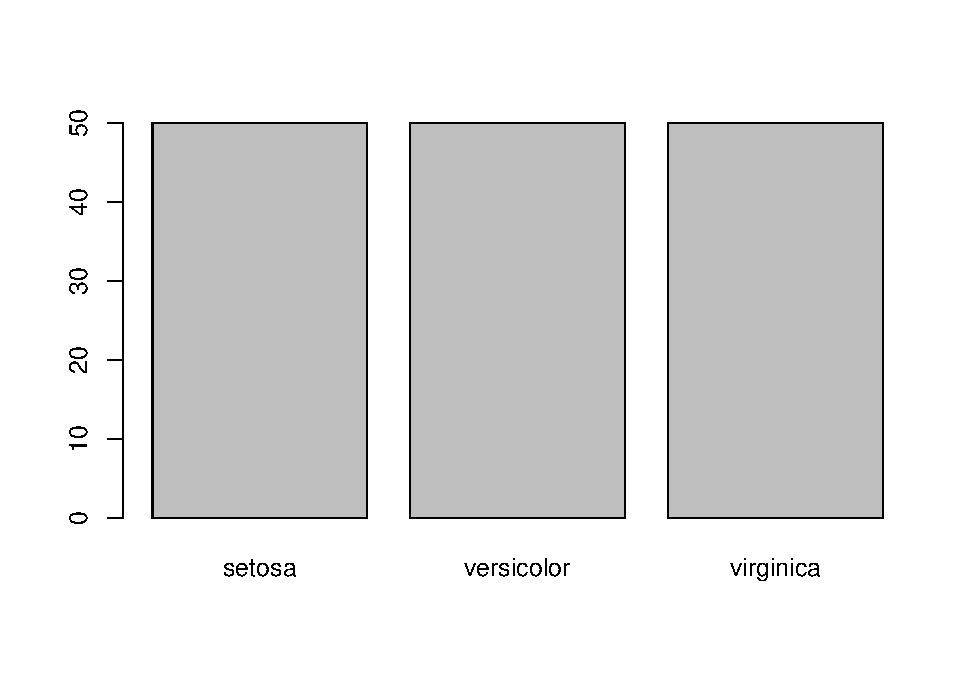
\includegraphics[width=1\linewidth]{01-introSo_files/figure-latex/unnamed-chunk-11-1} 

}

\caption{Tipos de gráficos}\label{fig:unnamed-chunk-11-1}
\end{figure}

\begin{Shaded}
\begin{Highlighting}[]
\CommentTok{\# Boxplot}
\FunctionTok{plot}\NormalTok{(iris}\SpecialCharTok{$}\NormalTok{Species, iris}\SpecialCharTok{$}\NormalTok{Sepal.Length,}
     \AttributeTok{xlab=}\StringTok{"Species"}\NormalTok{,}
     \AttributeTok{ylab=}\StringTok{"Sepal Lenght"}\NormalTok{,}
     \AttributeTok{main=}\StringTok{"Sepal Lenght by Iris species"}\NormalTok{,}
     \AttributeTok{col=}\StringTok{"skyblue"}\NormalTok{)}
\end{Highlighting}
\end{Shaded}

\begin{figure}

{\centering 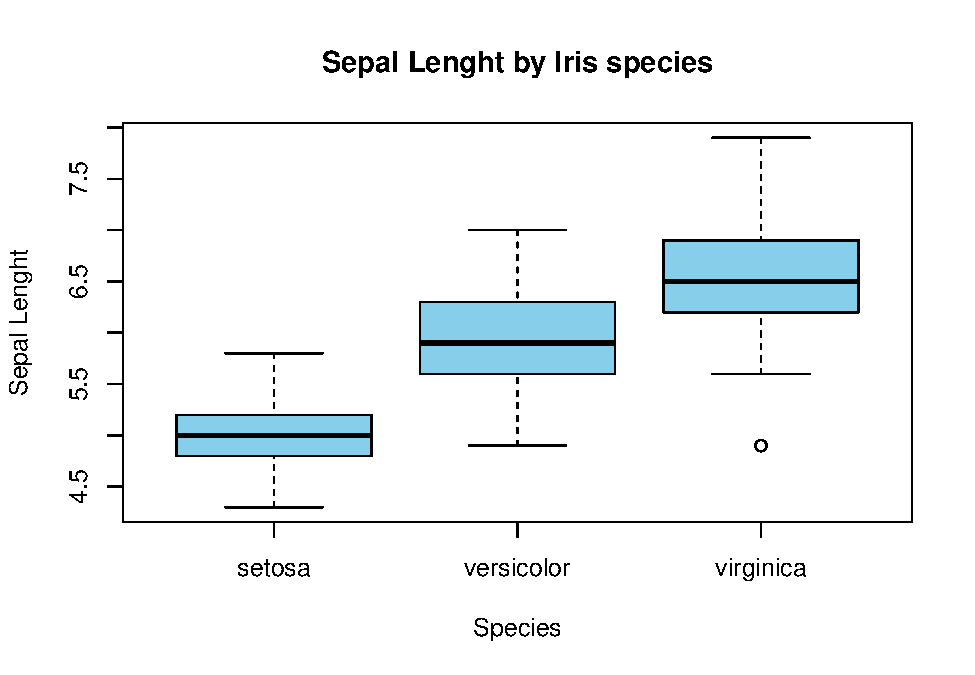
\includegraphics[width=1\linewidth]{01-introSo_files/figure-latex/unnamed-chunk-11-2} 

}

\caption{Tipos de gráficos}\label{fig:unnamed-chunk-11-2}
\end{figure}

\begin{Shaded}
\begin{Highlighting}[]
\CommentTok{\# Historgram}
\FunctionTok{hist}\NormalTok{(iris}\SpecialCharTok{$}\NormalTok{Sepal.Width,}
     \AttributeTok{col=}\StringTok{"yellow"}\NormalTok{,}
     \AttributeTok{xlab=}\StringTok{"Sepal Width"}\NormalTok{,}
     \AttributeTok{main=}\StringTok{"Histogram of Sepal Width"}\NormalTok{,}
     \AttributeTok{breaks=}\DecValTok{30}\NormalTok{)}
\end{Highlighting}
\end{Shaded}

\begin{figure}

{\centering 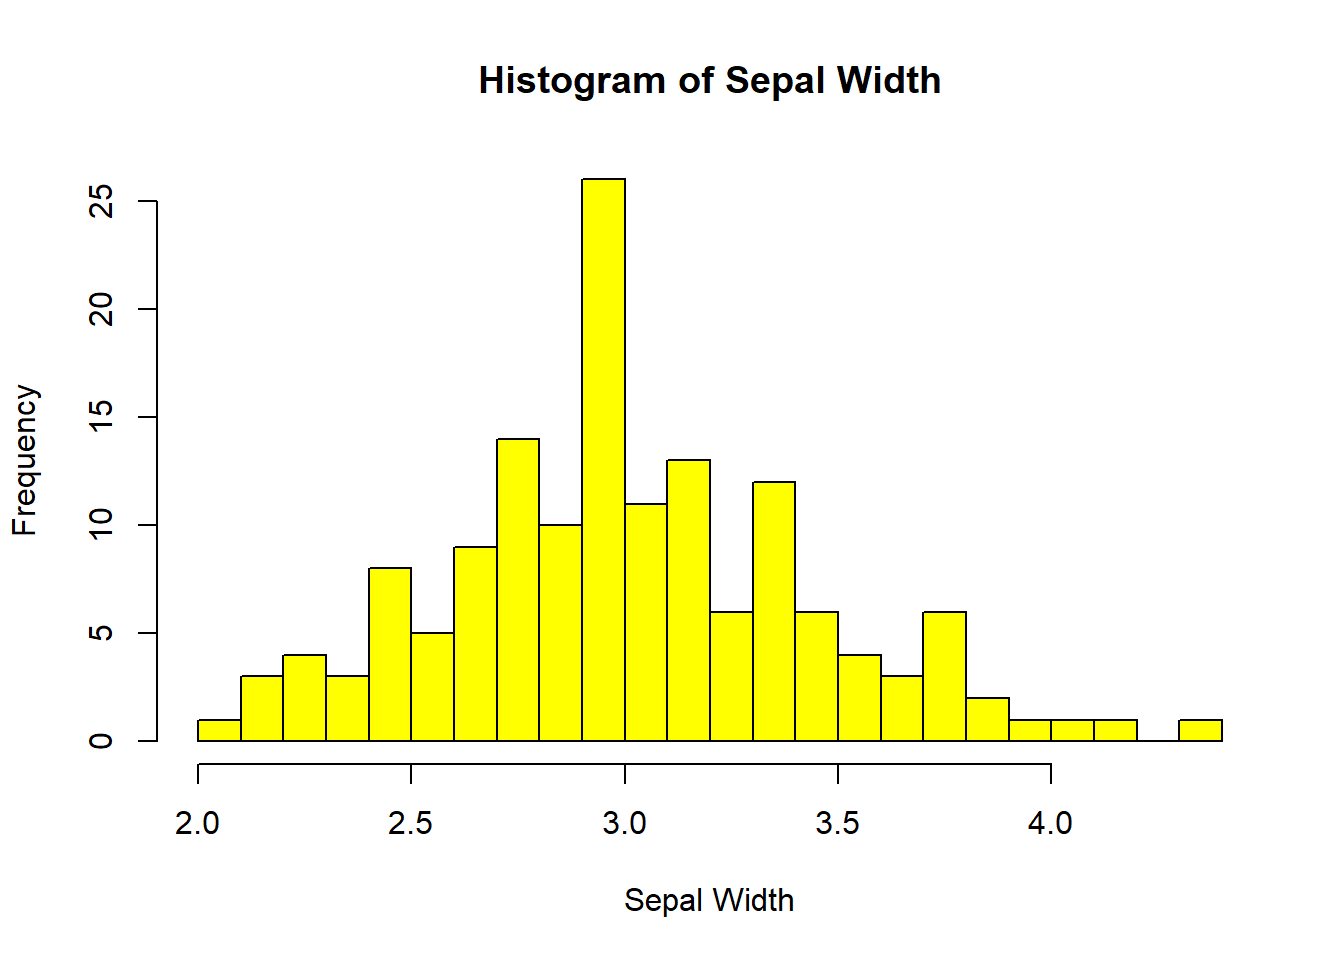
\includegraphics[width=1\linewidth]{01-introSo_files/figure-latex/unnamed-chunk-11-3} 

}

\caption{Tipos de gráficos}\label{fig:unnamed-chunk-11-3}
\end{figure}

\begin{Shaded}
\begin{Highlighting}[]
\CommentTok{\# Qué pasa si queremos plotear el data frame entero? }

\FunctionTok{plot}\NormalTok{(iris)}
\end{Highlighting}
\end{Shaded}

\begin{figure}

{\centering 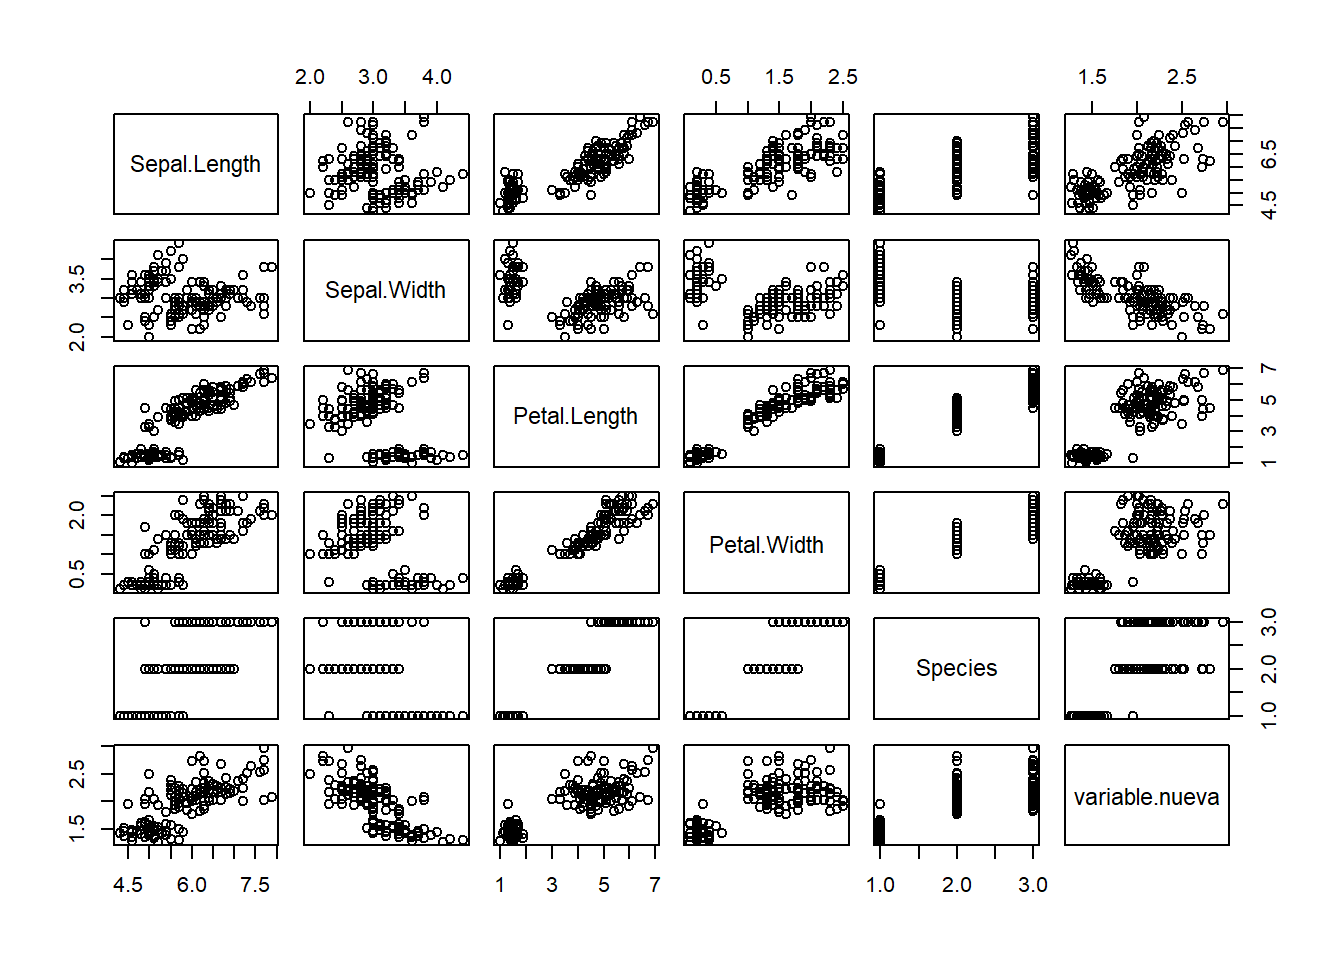
\includegraphics[width=1\linewidth]{01-introSo_files/figure-latex/unnamed-chunk-11-4} 

}

\caption{Tipos de gráficos}\label{fig:unnamed-chunk-11-4}
\end{figure}

\emph{ggplot2}

Este paquete tiene una manera de escribirse particular en capas. Los gráficos de ggplot2 está compuesto por los datos, por un conjunto de características estéticas a tener en cuenta entre los datos junto con los aspectos visuales (\emph{aes, aesthetic mapping}) y por al menos una capa que indica cómo se debe manipular cada observación (\emph{geom\_}).

\begin{Shaded}
\begin{Highlighting}[]
\FunctionTok{library}\NormalTok{(ggplot2)}

\FunctionTok{ggplot}\NormalTok{(iris, }\FunctionTok{aes}\NormalTok{(}\AttributeTok{x=}\NormalTok{Petal.Length, }\AttributeTok{y=}\NormalTok{Petal.Width))}\SpecialCharTok{+}
  \FunctionTok{geom\_point}\NormalTok{()}
\end{Highlighting}
\end{Shaded}

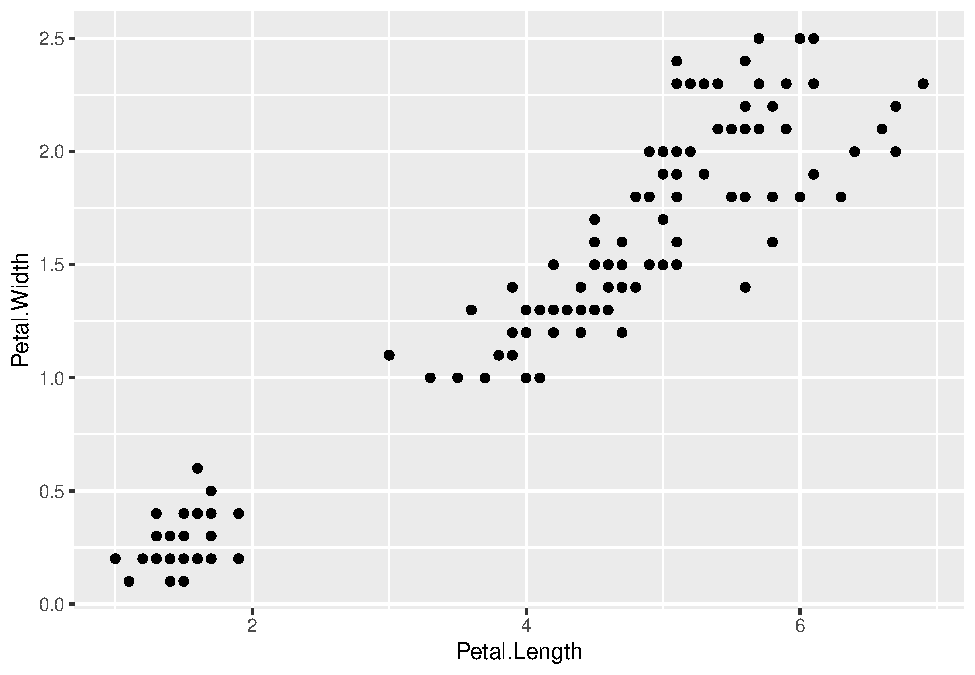
\includegraphics{01-introSo_files/figure-latex/unnamed-chunk-12-1.pdf}

\begin{itemize}
\tightlist
\item
  \textbf{Buenas prácticas!} Conviene usar un renglón por capa, de esta manera es fácil detectar errores y ver cómo se va modificando el gráfico a medida que van agregando capas.
\end{itemize}

Al igual que en el plot del R base, se pueden cambiar los colores y formas. Sin embargo, esto va a estar atado a qué elemento queremos cambiar.

\begin{Shaded}
\begin{Highlighting}[]
\FunctionTok{ggplot}\NormalTok{(iris, }\FunctionTok{aes}\NormalTok{(}\AttributeTok{x=}\NormalTok{Petal.Length, }\AttributeTok{y=}\NormalTok{Petal.Width))}\SpecialCharTok{+}
  \FunctionTok{geom\_point}\NormalTok{(}\FunctionTok{aes}\NormalTok{(}\AttributeTok{colour=}\NormalTok{Species)) }
\end{Highlighting}
\end{Shaded}

\includegraphics{01-introSo_files/figure-latex/unnamed-chunk-13-1.pdf}

En este caso, quise cambiar el color de los puntos. Para ello, lo tengo que especificar en la capa \emph{aes} del geom\_point.

\begin{Shaded}
\begin{Highlighting}[]
\FunctionTok{ggplot}\NormalTok{(iris, }\FunctionTok{aes}\NormalTok{(}\AttributeTok{x=}\NormalTok{Petal.Length, }\AttributeTok{y=}\NormalTok{Petal.Width, }\AttributeTok{color=}\NormalTok{Species))}\SpecialCharTok{+}
  \FunctionTok{geom\_point}\NormalTok{() }
\end{Highlighting}
\end{Shaded}

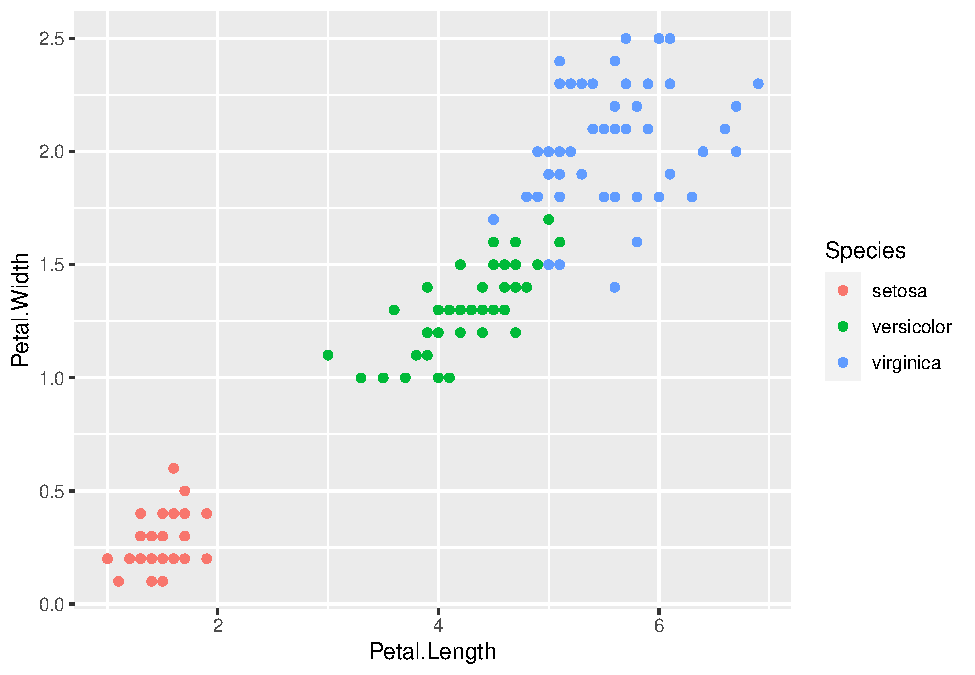
\includegraphics{01-introSo_files/figure-latex/unnamed-chunk-14-1.pdf}

También puede ir en el aes general del gráfico. No solo puedo cambiar el color, sino también formas. O combinar todo:

\begin{Shaded}
\begin{Highlighting}[]
\FunctionTok{ggplot}\NormalTok{(iris, }\FunctionTok{aes}\NormalTok{(}\AttributeTok{x=}\NormalTok{Petal.Length, }\AttributeTok{y=}\NormalTok{Petal.Width, }\AttributeTok{shape=}\NormalTok{Species))}\SpecialCharTok{+}
  \FunctionTok{geom\_point}\NormalTok{() }
\end{Highlighting}
\end{Shaded}

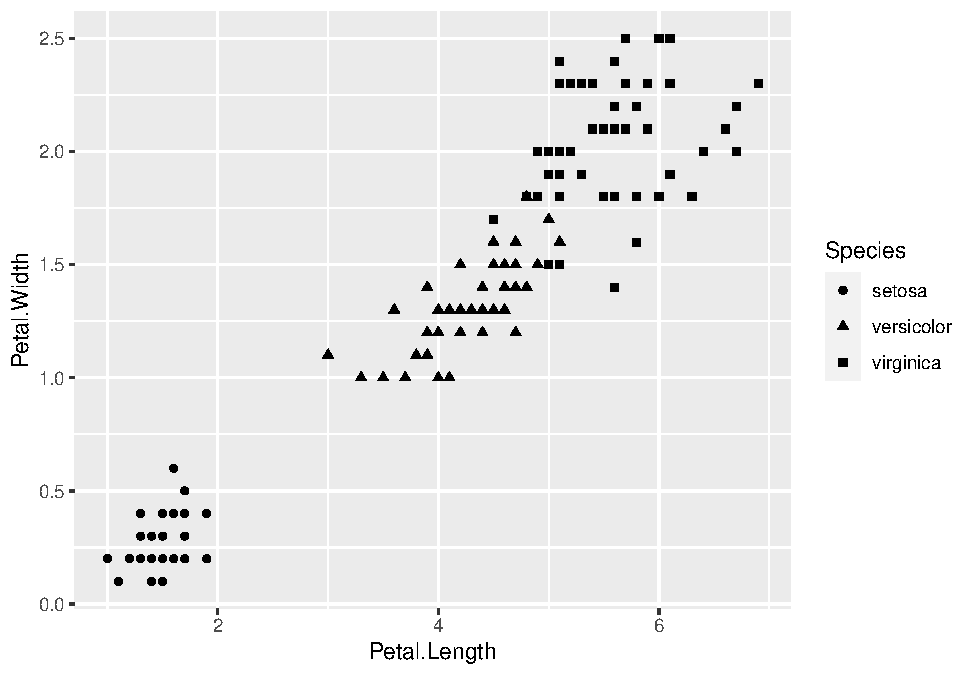
\includegraphics{01-introSo_files/figure-latex/unnamed-chunk-15-1.pdf}

\begin{Shaded}
\begin{Highlighting}[]
\FunctionTok{ggplot}\NormalTok{(iris, }\FunctionTok{aes}\NormalTok{(}\AttributeTok{x=}\NormalTok{Petal.Length, }\AttributeTok{y=}\NormalTok{Petal.Width, }\AttributeTok{size=}\NormalTok{Sepal.Length))}\SpecialCharTok{+}
  \FunctionTok{geom\_point}\NormalTok{(}\FunctionTok{aes}\NormalTok{(}\AttributeTok{color=}\NormalTok{Species)) }
\end{Highlighting}
\end{Shaded}

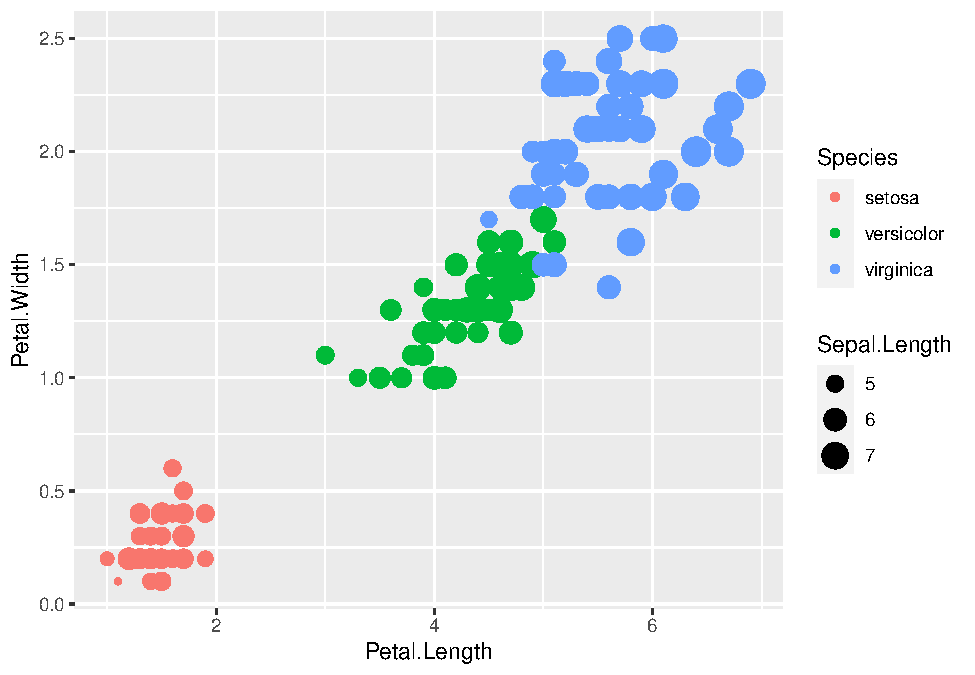
\includegraphics{01-introSo_files/figure-latex/unnamed-chunk-15-2.pdf}

Noten que se generan automáticamente las leyendas, según vamos cambiando lo estético, a diferencia de R base.

Este es un primer pantallazo el mundo de ggplot. Hay mucho para aprender y en general, todo lo que quieran graficar van a poder, y de muchisimas maneras.

Google es su gran amigo!

\hypertarget{recursos-extra-recomendados}{%
\subsection{Recursos extra recomendados}\label{recursos-extra-recomendados}}

Uso de la libreria \textbf{ggpubr} para alinear plots \url{http://www.sthda.com/english/articles/24-ggpubr-publication-ready-plots/81-ggplot2-easy-way-to-mix-multiple-graphs-on-the-same-page/}

Healy K. 2019. Data visualization: A practical Introduction \textbf{Versión libre online:}\\
\url{https://socviz.co/index.html\#preface}

R Charts \url{https://r-charts.com/es/ggplot2/}

Cheatsheet en Code \url{http://zevross.com/blog/2014/08/04/beautiful-plotting-in-r-a-ggplot2-cheatsheet-3}

\hypertarget{regmul}{%
\chapter{Correlaciones y regresión múltiple}\label{regmul}}

\emph{\textbf{Autora de esta unidad:} Natalia Morandeira}

En esta Unidad vamos a abordar análisis de correlación y regresiones múltiples (modelos lineales). Las correlaciones son análisis útiles para explorar nuestros datos y para evaluar si dos variables están asociadas positivamente o negativamente. Por otro lado, en el caso de una regresión simple, tenemos una variable respuesta (o dependiente) y una variable explicativa (o independiente). Un análisis de regresión múltiple es muy adecuado cuando hemos medido muchas variables, por ejemplo, si tenemos una variable respuesta y muchas posibles variables explicativas. Nos interesa conocer cuál o cuáles variables explican la variación de la variable respuesta, y elegir el mejor modelo.

En el marco de análisis limnológicos, una situación común es tener una variable respuesta medida en cuerpos de agua y múltiples variables que creemos que pueden explicar su variación. Entre las variables respuestas, podríamos tener (de acuerdo al objetivo de nuestro estudio) la abundancia, biomasa o diversidad de especies de un dado taxón o de grupos funcionales; o la concentración de un agroquímico; o incluso variables físico-químicas del cuerpo de agua que hipotetizamos que dependen de otro factor. Entre las variables respuestas, es posible que tengamos variables físico-químicas, características morfométricas de la laguna, usos de suelo del entorno, características de la cuenca, abundancia de otro taxón que interactúe con nuestra especie de interés, etc. Nos puede interesar en primer lugar analizar si están correlacionadas nuestras potenciales variables explicativas. Luego, podemos intentar ajustar un buen modelo que explique cómo varía nuestra variable respuesta en función de varias variables explicativas. Ese es el camino que recorreremos en esta Unidad.

\hypertarget{caso-de-estudio}{%
\section{Caso de estudio}\label{caso-de-estudio}}

El sitio de estudio es la turbera de Rancho Hambre (Tierra del Fuego, Argentina), en donde entre octubre de 2009 y abril de 2010 se realizaron muestreos en lagunas (ver \href{https://link.springer.com/article/10.1007/s10750-016-2969-2}{artículo} de Quiroga \emph{et al.} 2017, y la \href{http://hdl.handle.net/20.500.12110/tesis_n5433_Quiroga}{tesis doctoral} de María Victoria Quiroga (FCEN-UBA)). En cinco lagunas (RH1 a RH5), se realizaron muestreos estacionales (octubre, diciembre, febrero y abril), es decir, tenemos un total de 20 observaciones. Contamos con dos tablas de datos:

\begin{itemize}
\item
  \textbf{Datos limnológicos físicoquímicos.} Los datos corresponden a los sitios de muestreo de orilla de los cuerpos de agua. Los parámetros limnológicos fueron estimados según lo descripto en la sección \emph{Sampling regime, physical-chemical analyses} de Materiales y Métodos en Quiroga \emph{et al.} (2017). Los \href{http://hdl.handle.net/11336/201874}{datos físicoquímicos están disponibles en el repositorio digital de CONICET}. Consideraremos a las variables medidas como variables explicativas: pH, conductividad, oxígeno disuelto, dureza total, DOC, DIN, nitrógeno total, DRP, fósforo total, ag(440), SUVA254 e índice MS; todas ellas variables numéricas. Por otro lado tenemos variables categóricas que discutiremos cómo considerar: la laguna (cinco niveles) y la fecha de muestreo (cuatro niveles).
\item
  \textbf{Biomasa de morfotipos bacterianos}. La biomasa de bacterias heterótrofas se estimó utilizando microscopía de epifluorescencia y análisis de imágenes. Para detalles ver sección \emph{Bacterioplankton morphotypes} de Materiales y Métodos en Quiroga \emph{et al.} (2017). Los \href{http://hdl.handle.net/11336/201811}{datos de morfotipos bacterianos están disponibles en el repositorio digital de CONICET}. En la tabla se cuenta con la biomasa de seis morfotipos bacterianos distintos. Podemos tomar a la biomasa de cada morfotipo como una variable respuesta por separado, o bien considerar para un primer análisis a la biomasa total de bacterias heterótrofas como la variable a modelar.
\end{itemize}

\hypertarget{leer-y-emprolijar-los-datos}{%
\section{Leer y emprolijar los datos}\label{leer-y-emprolijar-los-datos}}

Siempre debemos mirar nuestra tabla de datos antes de empezar: detectar posibles errores o datos faltantes, retocar los nombres de las variables, agrupar filas y columnas si corresponde, etc. En nuestro caso además tenemos por un lado las variables físico-químicas y por el otro lado las variables biológicas, pero para los análisis es conveniente tener todos los datos en un mismo \emph{dataframe}.

Empezamos leyendo las bases de datos en R. Es una buena práctica guardar los archivos en una carpeta llamada \emph{data}, dentro de la carpeta de nuestro proyecto. Tenemos los datos en formato \emph{csv} en \href{https://github.com/Limno-con-R/CILCAL2023/tree/main/datasets}{GitHub Limno-con-R/CILCAL2023} \textbf{RH\_abiotic\_data.csv} y \textbf{RH\_morpho\_biomass.csv} (son casi iguales a los disponibles en el repositorio CONICET, se cambió un guión bajo por un espacio en una de las tablas). Cargamos los datos indicando que se saltee (\emph{skip}) la primera fila (¿por qué?).

\begin{Shaded}
\begin{Highlighting}[]
\FunctionTok{library}\NormalTok{(readr)}

\NormalTok{datos\_fq }\OtherTok{\textless{}{-}} \FunctionTok{read\_csv}\NormalTok{(}\StringTok{"data/RH\_abiotic\_data.csv"}\NormalTok{, }\AttributeTok{skip =} \DecValTok{1}\NormalTok{)}

\NormalTok{datos\_bacterias }\OtherTok{\textless{}{-}} \FunctionTok{read\_csv}\NormalTok{(}\StringTok{"data/RH\_morpho\_biomass.csv"}\NormalTok{, }\AttributeTok{skip =} \DecValTok{1}\NormalTok{)}
\end{Highlighting}
\end{Shaded}

Ahora vamos a ver los datos. Recordar o anotar cuántas filas y columnas tiene cada \emph{dataframe}.

\begin{Shaded}
\begin{Highlighting}[]
\NormalTok{datos\_fq}
\end{Highlighting}
\end{Shaded}

\begin{verbatim}
## # A tibble: 20 x 16
##    ID    Pool  Site      Date     pH Condu~1 Disso~2 Total~3   DOC   DIN Total~4
##    <chr> <chr> <chr>     <chr> <dbl>   <dbl>   <dbl>   <dbl> <dbl> <dbl>   <dbl>
##  1 1O    RH1   shore     Octo~  4.91    13.4    NA      21.2   5.6  83.6    1870
##  2 2O    RH2   shore     Octo~  5.52     8.7    NA      46.2   5.1  41.3    1980
##  3 3O    RH3   shore     Octo~  4.72    15.2    NA      13.8   2.8  10      1980
##  4 4O    RH4   north sh~ Octo~  5.09    11.8    NA      33.2   5.7  55.3    1650
##  5 5O    RH5   shore     Octo~  4.82     5.5    NA      25.8   3.9  54.4    3410
##  6 1D    RH1   shore     Dece~  6.39    19.1    11.0    38.5   7.2  21.1    1320
##  7 2D    RH2   shore     Dece~  4.75    22.6    11.0    42.1   7.7  12.1    1870
##  8 3D    RH3   shore     Dece~  4.67    26.7    11.7    18.9  13.4  22.6    5720
##  9 4D    RH4   north sh~ Dece~  6.75    25.6    11.7    24.8   5.3  34      7480
## 10 5D    RH5   shore     Dece~  4.65    23      11.5    20.1  11    11.2   10230
## 11 1F    RH1   shore     Febr~  5.9     21.4    10.4    39.5  12.7  53      8030
## 12 2F    RH2   shore     Febr~  5.19    22.6    10.2    34     5.9  30.3   10010
## 13 3F    RH3   shore     Febr~  4.66    25.7    10.6    32    12.5  45.3   11330
## 14 4F    RH4   north sh~ Febr~  6.65    26.8    10.9    36.6   4     0      5610
## 15 5F    RH5   shore     Febr~  4.82    27.2    10.4    24.5   7.1  22.3    8250
## 16 1A    RH1   shore     Apri~  7.1     21.4    10.7    25.3   7.6  23.1    9790
## 17 2A    RH2   shore     Apri~  4.88    24      11.4    20.3   7.5   0     11110
## 18 3A    RH3   shore     Apri~  5.4     28.5    10.4    18.8  12.7 103.     8910
## 19 4A    RH4   north sh~ Apri~  6.2     28.5    11.2    27.7   5.3  43      3630
## 20 5A    RH5   shore     Apri~  5.43    27.1    11.2    24.2  11.6  73.2    3740
## # ... with 5 more variables: DRP <dbl>, `Total phosphorus` <dbl>,
## #   `ag(440)` <dbl>, SUVA254 <dbl>, `MS index` <dbl>, and abbreviated variable
## #   names 1: Conductivity, 2: `Dissolved oxigen`, 3: `Total hardness`,
## #   4: `Total nitrogen`
\end{verbatim}

\begin{Shaded}
\begin{Highlighting}[]
\NormalTok{datos\_bacterias}
\end{Highlighting}
\end{Shaded}

\begin{verbatim}
## # A tibble: 20 x 10
##    ID    Pool  Site        Date  Filam~1 Large~2 Vibri~3 Large~4 Small~5 Small~6
##    <chr> <chr> <chr>       <chr>   <dbl>   <dbl>   <dbl>   <dbl>   <dbl>   <dbl>
##  1 1O    RH1   shore       Octo~       0   16921    5315   12676    1747   25994
##  2 2O    RH2   shore       Octo~    1435    5645    2384    7381     888   12075
##  3 3O    RH3   shore       Octo~   13307    1597     392    8131     708   13222
##  4 4O    RH4   north shore Octo~       0    8085    3499    7534    2028   25353
##  5 5O    RH5   shore       Octo~       0    1921     451   15662     666   31621
##  6 1D    RH1   shore       Dece~       0   12374    9228   21906    4503   38421
##  7 2D    RH2   shore       Dece~       0   22924    5933   34663    6687   77581
##  8 3D    RH3   shore       Dece~       0   12309    3471   46807    8694  139006
##  9 4D    RH4   north shore Dece~   44419   76819   19692   44391   24931  156132
## 10 5D    RH5   shore       Dece~       0   66952   23046  134707    2949  102890
## 11 1F    RH1   shore       Febr~    3177    6414    7533   22218    4013   34495
## 12 2F    RH2   shore       Febr~       0    7263    4879   25886    4098  137049
## 13 3F    RH3   shore       Febr~    3886    9283    1294   17402    2522   93008
## 14 4F    RH4   north shore Febr~    5860   54624   20331   33949   12469   58990
## 15 5F    RH5   shore       Febr~       0   21324   17482   24397    7064  106885
## 16 1A    RH1   shore       Apri~   12331   21098   11615   16083    6592   33478
## 17 2A    RH2   shore       Apri~       0    6950    4028   22525    1395   94037
## 18 3A    RH3   shore       Apri~       0   12394   17281   18608    4678  121090
## 19 4A    RH4   north shore Apri~       0     901    2484    3455     642   50957
## 20 5A    RH5   shore       Apri~       0    7626    3338   17231    2016   60287
## # ... with abbreviated variable names 1: Filaments, 2: Large_rods,
## #   3: Vibrio_shaped, 4: Large_cocci, 5: Small_rods, 6: Small_cocci
\end{verbatim}

Para unir estas tablas en una sola, debemos buscar una variable o columna que sea un indicador único de cada dato, y que sea equivalente en ambas tablas. ¿Cuál les parece que es?

Con ese indicador como nexo, haremos una \textbf{unión exterior completa} o \emph{full\_join}. Esto se debe a que queremos mantener todos los registros de nuestras tablas aunque para alguna laguna --quizás-- no hayamos podido medir los parámetros físicoquímicos o no hayamos podido medir la biomasa bacteriana. Para saber más sobre funciones que permiten relacionar conjuntos de datos, recomendamos consultar el capítulo \href{http://es.r4ds.hadley.nz/datos-relacionales.html}{13. Datos relacionales} (en particular \emph{13.4.1. Entendiendo las uniones}) en el libro traducido a castellano \href{http://es.r4ds.hadley.nz/}{R para Ciencias de Datos}, de Hadley Wickham y Garret Grolemund (2017).

Hacemos la unión e inspeccionamos la tabla (¿cuántas filas y columnas tiene?).

\begin{Shaded}
\begin{Highlighting}[]
\FunctionTok{library}\NormalTok{(tidyverse)}
\end{Highlighting}
\end{Shaded}

\begin{Shaded}
\begin{Highlighting}[]
\NormalTok{datos\_RH }\OtherTok{\textless{}{-}} \FunctionTok{full\_join}\NormalTok{(datos\_bacterias, datos\_fq, }\AttributeTok{by =} \StringTok{"ID"}\NormalTok{)}
\NormalTok{datos\_RH }
\end{Highlighting}
\end{Shaded}

\begin{verbatim}
## # A tibble: 20 x 25
##    ID    Pool.x Site.x    Date.x Filam~1 Large~2 Vibri~3 Large~4 Small~5 Small~6
##    <chr> <chr>  <chr>     <chr>    <dbl>   <dbl>   <dbl>   <dbl>   <dbl>   <dbl>
##  1 1O    RH1    shore     Octob~       0   16921    5315   12676    1747   25994
##  2 2O    RH2    shore     Octob~    1435    5645    2384    7381     888   12075
##  3 3O    RH3    shore     Octob~   13307    1597     392    8131     708   13222
##  4 4O    RH4    north sh~ Octob~       0    8085    3499    7534    2028   25353
##  5 5O    RH5    shore     Octob~       0    1921     451   15662     666   31621
##  6 1D    RH1    shore     Decem~       0   12374    9228   21906    4503   38421
##  7 2D    RH2    shore     Decem~       0   22924    5933   34663    6687   77581
##  8 3D    RH3    shore     Decem~       0   12309    3471   46807    8694  139006
##  9 4D    RH4    north sh~ Decem~   44419   76819   19692   44391   24931  156132
## 10 5D    RH5    shore     Decem~       0   66952   23046  134707    2949  102890
## 11 1F    RH1    shore     Febru~    3177    6414    7533   22218    4013   34495
## 12 2F    RH2    shore     Febru~       0    7263    4879   25886    4098  137049
## 13 3F    RH3    shore     Febru~    3886    9283    1294   17402    2522   93008
## 14 4F    RH4    north sh~ Febru~    5860   54624   20331   33949   12469   58990
## 15 5F    RH5    shore     Febru~       0   21324   17482   24397    7064  106885
## 16 1A    RH1    shore     April~   12331   21098   11615   16083    6592   33478
## 17 2A    RH2    shore     April~       0    6950    4028   22525    1395   94037
## 18 3A    RH3    shore     April~       0   12394   17281   18608    4678  121090
## 19 4A    RH4    north sh~ April~       0     901    2484    3455     642   50957
## 20 5A    RH5    shore     April~       0    7626    3338   17231    2016   60287
## # ... with 15 more variables: Pool.y <chr>, Site.y <chr>, Date.y <chr>,
## #   pH <dbl>, Conductivity <dbl>, `Dissolved oxigen` <dbl>,
## #   `Total hardness` <dbl>, DOC <dbl>, DIN <dbl>, `Total nitrogen` <dbl>,
## #   DRP <dbl>, `Total phosphorus` <dbl>, `ag(440)` <dbl>, SUVA254 <dbl>,
## #   `MS index` <dbl>, and abbreviated variable names 1: Filaments,
## #   2: Large_rods, 3: Vibrio_shaped, 4: Large_cocci, 5: Small_rods,
## #   6: Small_cocci
\end{verbatim}

Las variables Pool, Site y Date se repiten en ambas tablas, por eso aparecen como Pool.x y Pool.y (por ejemplo). Dado que son idénticas, tenemos la opción de eliminar estas variables de alguna de las dos tablas, o bien incluirlas como parte de la información de nexo.

\begin{Shaded}
\begin{Highlighting}[]
\NormalTok{datos\_RH }\OtherTok{\textless{}{-}} \FunctionTok{full\_join}\NormalTok{(datos\_bacterias, datos\_fq, }\AttributeTok{by =} \FunctionTok{c}\NormalTok{(}\StringTok{"ID"}\NormalTok{, }\StringTok{"Pool"}\NormalTok{, }\StringTok{"Site"}\NormalTok{, }\StringTok{"Date"}\NormalTok{))}
\NormalTok{datos\_RH }
\end{Highlighting}
\end{Shaded}

\begin{verbatim}
## # A tibble: 20 x 22
##    ID    Pool  Site  Date  Filam~1 Large~2 Vibri~3 Large~4 Small~5 Small~6    pH
##    <chr> <chr> <chr> <chr>   <dbl>   <dbl>   <dbl>   <dbl>   <dbl>   <dbl> <dbl>
##  1 1O    RH1   shore Octo~       0   16921    5315   12676    1747   25994  4.91
##  2 2O    RH2   shore Octo~    1435    5645    2384    7381     888   12075  5.52
##  3 3O    RH3   shore Octo~   13307    1597     392    8131     708   13222  4.72
##  4 4O    RH4   nort~ Octo~       0    8085    3499    7534    2028   25353  5.09
##  5 5O    RH5   shore Octo~       0    1921     451   15662     666   31621  4.82
##  6 1D    RH1   shore Dece~       0   12374    9228   21906    4503   38421  6.39
##  7 2D    RH2   shore Dece~       0   22924    5933   34663    6687   77581  4.75
##  8 3D    RH3   shore Dece~       0   12309    3471   46807    8694  139006  4.67
##  9 4D    RH4   nort~ Dece~   44419   76819   19692   44391   24931  156132  6.75
## 10 5D    RH5   shore Dece~       0   66952   23046  134707    2949  102890  4.65
## 11 1F    RH1   shore Febr~    3177    6414    7533   22218    4013   34495  5.9 
## 12 2F    RH2   shore Febr~       0    7263    4879   25886    4098  137049  5.19
## 13 3F    RH3   shore Febr~    3886    9283    1294   17402    2522   93008  4.66
## 14 4F    RH4   nort~ Febr~    5860   54624   20331   33949   12469   58990  6.65
## 15 5F    RH5   shore Febr~       0   21324   17482   24397    7064  106885  4.82
## 16 1A    RH1   shore Apri~   12331   21098   11615   16083    6592   33478  7.1 
## 17 2A    RH2   shore Apri~       0    6950    4028   22525    1395   94037  4.88
## 18 3A    RH3   shore Apri~       0   12394   17281   18608    4678  121090  5.4 
## 19 4A    RH4   nort~ Apri~       0     901    2484    3455     642   50957  6.2 
## 20 5A    RH5   shore Apri~       0    7626    3338   17231    2016   60287  5.43
## # ... with 11 more variables: Conductivity <dbl>, `Dissolved oxigen` <dbl>,
## #   `Total hardness` <dbl>, DOC <dbl>, DIN <dbl>, `Total nitrogen` <dbl>,
## #   DRP <dbl>, `Total phosphorus` <dbl>, `ag(440)` <dbl>, SUVA254 <dbl>,
## #   `MS index` <dbl>, and abbreviated variable names 1: Filaments,
## #   2: Large_rods, 3: Vibrio_shaped, 4: Large_cocci, 5: Small_rods,
## #   6: Small_cocci
\end{verbatim}

Ahora vamos a mejorar los nombres de las columnas. Una buena práctica es elegir siempre el mismo tipo de nomenclatura. Hay varias convenciones pero las más elegidas en el mundo de R son \textbf{\emph{snake}} y \textbf{\emph{camel}}. La nomenclatura \emph{snake} implica usar guiones bajos como separador de palabras y, generalmente, todas las letras en minúscula. La nomenclatura \emph{camel} implica, en vez de usar guiones, usar a las mayúsculas como indicador de que hay una palabra nueva, y siempre dejar a la primera palabra en minúscula. Si nuestra variable se llama ``Fecha de muestreo'', la nomenclatura sería \emph{fecha\_de\_muestreo} o \emph{fechaDeMuestreo}, de acuerdo a la convención elegida.

En la tabla que tenemos, hay una mezcla de criterios: se usan guiones bajos pero a la vez las variables empiezan con mayúscula. Vamos a ajustar. Vamos a pasar todas las variables al formato \emph{snake} con una función muy útil, que también sirve para nombres de columnas más desprolijos (por ejemplo, si tenemos otros signos de puntuación en los nombres).

\begin{Shaded}
\begin{Highlighting}[]
\FunctionTok{library}\NormalTok{(janitor)}
\end{Highlighting}
\end{Shaded}

\begin{Shaded}
\begin{Highlighting}[]
\NormalTok{datos\_RH }\OtherTok{\textless{}{-}} \FunctionTok{clean\_names}\NormalTok{(datos\_RH)}
\NormalTok{datos\_RH }
\end{Highlighting}
\end{Shaded}

\begin{verbatim}
## # A tibble: 20 x 22
##    id    pool  site  date  filam~1 large~2 vibri~3 large~4 small~5 small~6   p_h
##    <chr> <chr> <chr> <chr>   <dbl>   <dbl>   <dbl>   <dbl>   <dbl>   <dbl> <dbl>
##  1 1O    RH1   shore Octo~       0   16921    5315   12676    1747   25994  4.91
##  2 2O    RH2   shore Octo~    1435    5645    2384    7381     888   12075  5.52
##  3 3O    RH3   shore Octo~   13307    1597     392    8131     708   13222  4.72
##  4 4O    RH4   nort~ Octo~       0    8085    3499    7534    2028   25353  5.09
##  5 5O    RH5   shore Octo~       0    1921     451   15662     666   31621  4.82
##  6 1D    RH1   shore Dece~       0   12374    9228   21906    4503   38421  6.39
##  7 2D    RH2   shore Dece~       0   22924    5933   34663    6687   77581  4.75
##  8 3D    RH3   shore Dece~       0   12309    3471   46807    8694  139006  4.67
##  9 4D    RH4   nort~ Dece~   44419   76819   19692   44391   24931  156132  6.75
## 10 5D    RH5   shore Dece~       0   66952   23046  134707    2949  102890  4.65
## 11 1F    RH1   shore Febr~    3177    6414    7533   22218    4013   34495  5.9 
## 12 2F    RH2   shore Febr~       0    7263    4879   25886    4098  137049  5.19
## 13 3F    RH3   shore Febr~    3886    9283    1294   17402    2522   93008  4.66
## 14 4F    RH4   nort~ Febr~    5860   54624   20331   33949   12469   58990  6.65
## 15 5F    RH5   shore Febr~       0   21324   17482   24397    7064  106885  4.82
## 16 1A    RH1   shore Apri~   12331   21098   11615   16083    6592   33478  7.1 
## 17 2A    RH2   shore Apri~       0    6950    4028   22525    1395   94037  4.88
## 18 3A    RH3   shore Apri~       0   12394   17281   18608    4678  121090  5.4 
## 19 4A    RH4   nort~ Apri~       0     901    2484    3455     642   50957  6.2 
## 20 5A    RH5   shore Apri~       0    7626    3338   17231    2016   60287  5.43
## # ... with 11 more variables: conductivity <dbl>, dissolved_oxigen <dbl>,
## #   total_hardness <dbl>, doc <dbl>, din <dbl>, total_nitrogen <dbl>,
## #   drp <dbl>, total_phosphorus <dbl>, ag_440 <dbl>, suva254 <dbl>,
## #   ms_index <dbl>, and abbreviated variable names 1: filaments, 2: large_rods,
## #   3: vibrio_shaped, 4: large_cocci, 5: small_rods, 6: small_cocci
\end{verbatim}

El nombre de la variable pH quedó un poco raro, lo vamos a cambiar. A continuación se pide el nombre de las columnas de datos\_RH, luego específicamente el de la columna 11, y luego lo cambiamos.

\begin{Shaded}
\begin{Highlighting}[]
\FunctionTok{colnames}\NormalTok{(datos\_RH)}
\end{Highlighting}
\end{Shaded}

\begin{verbatim}
##  [1] "id"               "pool"             "site"             "date"            
##  [5] "filaments"        "large_rods"       "vibrio_shaped"    "large_cocci"     
##  [9] "small_rods"       "small_cocci"      "p_h"              "conductivity"    
## [13] "dissolved_oxigen" "total_hardness"   "doc"              "din"             
## [17] "total_nitrogen"   "drp"              "total_phosphorus" "ag_440"          
## [21] "suva254"          "ms_index"
\end{verbatim}

\begin{Shaded}
\begin{Highlighting}[]
\FunctionTok{colnames}\NormalTok{(datos\_RH)[}\DecValTok{11}\NormalTok{]}
\end{Highlighting}
\end{Shaded}

\begin{verbatim}
## [1] "p_h"
\end{verbatim}

\begin{Shaded}
\begin{Highlighting}[]
\FunctionTok{colnames}\NormalTok{(datos\_RH)[}\DecValTok{11}\NormalTok{] }\OtherTok{\textless{}{-}} \StringTok{"ph"}
\FunctionTok{colnames}\NormalTok{(datos\_RH)}
\end{Highlighting}
\end{Shaded}

\begin{verbatim}
##  [1] "id"               "pool"             "site"             "date"            
##  [5] "filaments"        "large_rods"       "vibrio_shaped"    "large_cocci"     
##  [9] "small_rods"       "small_cocci"      "ph"               "conductivity"    
## [13] "dissolved_oxigen" "total_hardness"   "doc"              "din"             
## [17] "total_nitrogen"   "drp"              "total_phosphorus" "ag_440"          
## [21] "suva254"          "ms_index"
\end{verbatim}

Finalmente, vamos a agregar una nueva columna con la biomasa total bacteriana. Existen múltiples métodos para hacer esto, vamos a ver dos, uno con la sintaxis base de R y otro con la sintaxis de \emph{tidyverse}. Para conocer más sobre los tipos de sintaxis de R, recomendamos la hoja de referencia \href{https://raw.githubusercontent.com/rstudio/cheatsheets/main/translations/spanish/syntax_es.pdf}{Comparación de sintaxis de R}, por Amelia McNamara (traducida al castellano por RLadies).

\begin{Shaded}
\begin{Highlighting}[]
\CommentTok{\#Con la sintaxis base}
\NormalTok{datos\_bio\_opcion1 }\OtherTok{\textless{}{-}}\NormalTok{ datos\_RH }\CommentTok{\#duplico el dataframe para no sobreescribirlo y comparar los resultados}

\NormalTok{datos\_bio\_opcion1}\SpecialCharTok{$}\NormalTok{bio\_total }\OtherTok{\textless{}{-}}\NormalTok{ datos\_bio\_opcion1}\SpecialCharTok{$}\NormalTok{filaments }\SpecialCharTok{+}\NormalTok{ datos\_bio\_opcion1}\SpecialCharTok{$}\NormalTok{large\_rods }\SpecialCharTok{+}\NormalTok{ datos\_bio\_opcion1}\SpecialCharTok{$}\NormalTok{vibrio\_shaped }\SpecialCharTok{+}\NormalTok{ datos\_bio\_opcion1}\SpecialCharTok{$}\NormalTok{large\_cocci }\SpecialCharTok{+}\NormalTok{ datos\_bio\_opcion1}\SpecialCharTok{$}\NormalTok{small\_rods }\SpecialCharTok{+}\NormalTok{ datos\_bio\_opcion1}\SpecialCharTok{$}\NormalTok{small\_cocci}

\NormalTok{datos\_bio\_opcion1}
\end{Highlighting}
\end{Shaded}

\begin{verbatim}
## # A tibble: 20 x 23
##    id    pool  site  date  filam~1 large~2 vibri~3 large~4 small~5 small~6    ph
##    <chr> <chr> <chr> <chr>   <dbl>   <dbl>   <dbl>   <dbl>   <dbl>   <dbl> <dbl>
##  1 1O    RH1   shore Octo~       0   16921    5315   12676    1747   25994  4.91
##  2 2O    RH2   shore Octo~    1435    5645    2384    7381     888   12075  5.52
##  3 3O    RH3   shore Octo~   13307    1597     392    8131     708   13222  4.72
##  4 4O    RH4   nort~ Octo~       0    8085    3499    7534    2028   25353  5.09
##  5 5O    RH5   shore Octo~       0    1921     451   15662     666   31621  4.82
##  6 1D    RH1   shore Dece~       0   12374    9228   21906    4503   38421  6.39
##  7 2D    RH2   shore Dece~       0   22924    5933   34663    6687   77581  4.75
##  8 3D    RH3   shore Dece~       0   12309    3471   46807    8694  139006  4.67
##  9 4D    RH4   nort~ Dece~   44419   76819   19692   44391   24931  156132  6.75
## 10 5D    RH5   shore Dece~       0   66952   23046  134707    2949  102890  4.65
## 11 1F    RH1   shore Febr~    3177    6414    7533   22218    4013   34495  5.9 
## 12 2F    RH2   shore Febr~       0    7263    4879   25886    4098  137049  5.19
## 13 3F    RH3   shore Febr~    3886    9283    1294   17402    2522   93008  4.66
## 14 4F    RH4   nort~ Febr~    5860   54624   20331   33949   12469   58990  6.65
## 15 5F    RH5   shore Febr~       0   21324   17482   24397    7064  106885  4.82
## 16 1A    RH1   shore Apri~   12331   21098   11615   16083    6592   33478  7.1 
## 17 2A    RH2   shore Apri~       0    6950    4028   22525    1395   94037  4.88
## 18 3A    RH3   shore Apri~       0   12394   17281   18608    4678  121090  5.4 
## 19 4A    RH4   nort~ Apri~       0     901    2484    3455     642   50957  6.2 
## 20 5A    RH5   shore Apri~       0    7626    3338   17231    2016   60287  5.43
## # ... with 12 more variables: conductivity <dbl>, dissolved_oxigen <dbl>,
## #   total_hardness <dbl>, doc <dbl>, din <dbl>, total_nitrogen <dbl>,
## #   drp <dbl>, total_phosphorus <dbl>, ag_440 <dbl>, suva254 <dbl>,
## #   ms_index <dbl>, bio_total <dbl>, and abbreviated variable names
## #   1: filaments, 2: large_rods, 3: vibrio_shaped, 4: large_cocci,
## #   5: small_rods, 6: small_cocci
\end{verbatim}

\begin{Shaded}
\begin{Highlighting}[]
\CommentTok{\#Con la sintaxis tidyverse, la cual usa el operador \_pipe\_ ("la pipa") \%\textgreater{}\%}

\NormalTok{datos\_bio\_opcion2 }\OtherTok{\textless{}{-}}\NormalTok{ datos\_RH }\SpecialCharTok{\%\textgreater{}\%}
  \FunctionTok{mutate}\NormalTok{(}\AttributeTok{bio\_total =}\NormalTok{ filaments }\SpecialCharTok{+}\NormalTok{ large\_rods }\SpecialCharTok{+}\NormalTok{ vibrio\_shaped }\SpecialCharTok{+}\NormalTok{ large\_cocci }\SpecialCharTok{+}\NormalTok{ small\_rods }\SpecialCharTok{+}\NormalTok{ small\_cocci, }\AttributeTok{.before=}\NormalTok{filaments)}

\NormalTok{datos\_bio\_opcion2}
\end{Highlighting}
\end{Shaded}

\begin{verbatim}
## # A tibble: 20 x 23
##    id    pool  site        date  bio_t~1 filam~2 large~3 vibri~4 large~5 small~6
##    <chr> <chr> <chr>       <chr>   <dbl>   <dbl>   <dbl>   <dbl>   <dbl>   <dbl>
##  1 1O    RH1   shore       Octo~   62653       0   16921    5315   12676    1747
##  2 2O    RH2   shore       Octo~   29808    1435    5645    2384    7381     888
##  3 3O    RH3   shore       Octo~   37357   13307    1597     392    8131     708
##  4 4O    RH4   north shore Octo~   46499       0    8085    3499    7534    2028
##  5 5O    RH5   shore       Octo~   50321       0    1921     451   15662     666
##  6 1D    RH1   shore       Dece~   86432       0   12374    9228   21906    4503
##  7 2D    RH2   shore       Dece~  147788       0   22924    5933   34663    6687
##  8 3D    RH3   shore       Dece~  210287       0   12309    3471   46807    8694
##  9 4D    RH4   north shore Dece~  366384   44419   76819   19692   44391   24931
## 10 5D    RH5   shore       Dece~  330544       0   66952   23046  134707    2949
## 11 1F    RH1   shore       Febr~   77850    3177    6414    7533   22218    4013
## 12 2F    RH2   shore       Febr~  179175       0    7263    4879   25886    4098
## 13 3F    RH3   shore       Febr~  127395    3886    9283    1294   17402    2522
## 14 4F    RH4   north shore Febr~  186223    5860   54624   20331   33949   12469
## 15 5F    RH5   shore       Febr~  177152       0   21324   17482   24397    7064
## 16 1A    RH1   shore       Apri~  101197   12331   21098   11615   16083    6592
## 17 2A    RH2   shore       Apri~  128935       0    6950    4028   22525    1395
## 18 3A    RH3   shore       Apri~  174051       0   12394   17281   18608    4678
## 19 4A    RH4   north shore Apri~   58439       0     901    2484    3455     642
## 20 5A    RH5   shore       Apri~   90498       0    7626    3338   17231    2016
## # ... with 13 more variables: small_cocci <dbl>, ph <dbl>, conductivity <dbl>,
## #   dissolved_oxigen <dbl>, total_hardness <dbl>, doc <dbl>, din <dbl>,
## #   total_nitrogen <dbl>, drp <dbl>, total_phosphorus <dbl>, ag_440 <dbl>,
## #   suva254 <dbl>, ms_index <dbl>, and abbreviated variable names 1: bio_total,
## #   2: filaments, 3: large_rods, 4: vibrio_shaped, 5: large_cocci,
## #   6: small_rods
\end{verbatim}

La ventaja de la segunda opción es que podemos elegir dónde agregar la nueva columna (antes de la columna \emph{filaments}, por ejemplo). Así que nos quedaremos con esta tabla para los siguientes pasos. De paso, borramos los dataframes que ya no necesitamos.

\begin{Shaded}
\begin{Highlighting}[]
\NormalTok{datos\_RH }\OtherTok{\textless{}{-}}\NormalTok{ datos\_bio\_opcion2}

\FunctionTok{rm}\NormalTok{(datos\_bio\_opcion2)}
\FunctionTok{rm}\NormalTok{(datos\_bio\_opcion1)}
\end{Highlighting}
\end{Shaded}

Un último paso es informar que las variables pool y date son categóricas (factores). En el caso de date, además es adecuado ordenar los niveles de los factores, tanto para algunos análisis que consideren el orden de los meses (aquí nos exceden) como para mejorar la forma en que resumimos los resultados en una tabla o en un gráfico.

\begin{Shaded}
\begin{Highlighting}[]
\NormalTok{datos\_RH}\SpecialCharTok{$}\NormalTok{pool }\OtherTok{\textless{}{-}} \FunctionTok{factor}\NormalTok{(datos\_RH}\SpecialCharTok{$}\NormalTok{pool) }\CommentTok{\#en este caso no indicamos los niveles, ya que el orden alfabético es adecuado}

\NormalTok{datos\_RH}\SpecialCharTok{$}\NormalTok{date }\OtherTok{\textless{}{-}} \FunctionTok{factor}\NormalTok{(datos\_RH}\SpecialCharTok{$}\NormalTok{date, }\AttributeTok{levels =} \FunctionTok{c}\NormalTok{(}\StringTok{"October\_2009"}\NormalTok{, }\StringTok{"December\_2009"}\NormalTok{, }\StringTok{"February\_2010"}\NormalTok{, }\StringTok{"April\_2010"}\NormalTok{))}
\end{Highlighting}
\end{Shaded}

¡Listo! Podemos empezar con los análisis.

\hypertarget{correlaciones}{%
\section{Correlaciones}\label{correlaciones}}

Primero vamos a realizar análisis rápidos de todos los pares de variables con la librería \emph{GGally}.

\begin{Shaded}
\begin{Highlighting}[]
\FunctionTok{library}\NormalTok{(GGally)}
\end{Highlighting}
\end{Shaded}

\hypertarget{entre-biomasa-de-morfotipos-bacterianos}{%
\subsection{Entre biomasa de morfotipos bacterianos}\label{entre-biomasa-de-morfotipos-bacterianos}}

Vamos a analizar en primer lugar las variables biológicas, para lo cual generamos un nuevo dataframe que es un subconjunto de los anteriores.

\begin{Shaded}
\begin{Highlighting}[]
\NormalTok{datos\_bacterias }\OtherTok{\textless{}{-}}\NormalTok{ datos\_RH[,}\DecValTok{5}\SpecialCharTok{:}\DecValTok{11}\NormalTok{]}
  
\FunctionTok{ggpairs}\NormalTok{(datos\_bacterias, }\AttributeTok{title=}\StringTok{"Correlograma entre la biomasa de morfotipos bacterianos"}\NormalTok{) }
\end{Highlighting}
\end{Shaded}

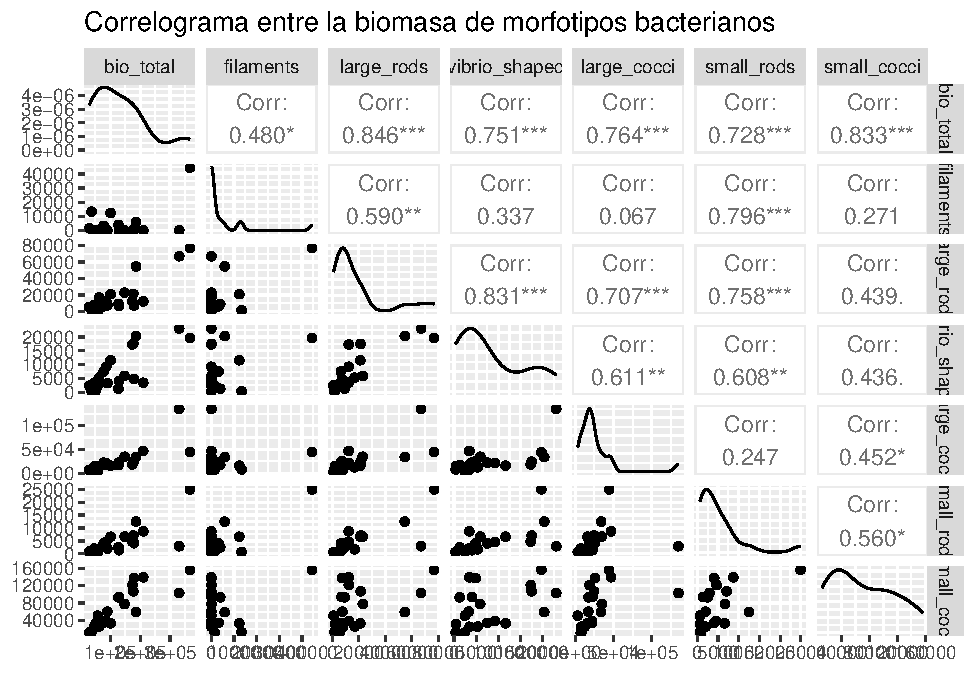
\includegraphics{02-RegMult_files/figure-latex/correlo1-1.pdf}
Obtenemos una matriz de gráficos, en la que cada celda expresa la correlacion de un par de variables. En este caso, todas las variables son continuas, por lo que observamos que los gráficos en la parte inferior de la matriz son de dispersión (puntos).

En las diagonales, observamos histogramas suavizados para cada variable. Por ejemplo, comparemos el histograma de la biomasa total.

\begin{Shaded}
\begin{Highlighting}[]
\FunctionTok{hist}\NormalTok{(datos\_bacterias}\SpecialCharTok{$}\NormalTok{bio\_total, }\AttributeTok{breaks=}\DecValTok{10}\NormalTok{, }\AttributeTok{col=}\StringTok{"lightblue"}\NormalTok{, }\AttributeTok{xlab=}\StringTok{"Biomasa total de bacterias heterótrofas"}\NormalTok{, }\AttributeTok{ylab=}\StringTok{"Frecuencia"}\NormalTok{, }\AttributeTok{main=}\StringTok{""}\NormalTok{)}
\end{Highlighting}
\end{Shaded}

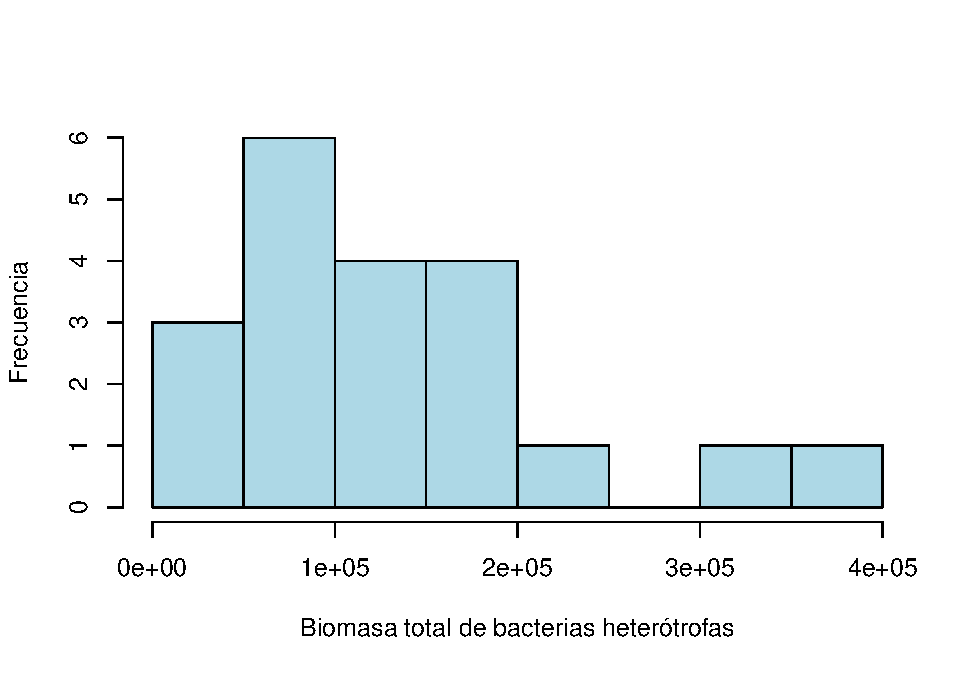
\includegraphics{02-RegMult_files/figure-latex/hist-1.pdf}

En la parte superior, se muestra el coeficiente de correlación para cada par de variables y asteriscos indicando su nivel de significancia. Podemos evaluar el par que nos interese con una función, para tener información numérica más detallada.

\begin{Shaded}
\begin{Highlighting}[]
\FunctionTok{cor.test}\NormalTok{(datos\_bacterias}\SpecialCharTok{$}\NormalTok{vibrio\_shaped, datos\_bacterias}\SpecialCharTok{$}\NormalTok{large\_rods)}
\end{Highlighting}
\end{Shaded}

\begin{verbatim}
## 
##  Pearson's product-moment correlation
## 
## data:  datos_bacterias$vibrio_shaped and datos_bacterias$large_rods
## t = 6.3382, df = 18, p-value = 5.68e-06
## alternative hypothesis: true correlation is not equal to 0
## 95 percent confidence interval:
##  0.6144454 0.9311213
## sample estimates:
##       cor 
## 0.8310104
\end{verbatim}

Aquí observamos que el coeficiente de la correlación de Pearson es r = 0.8310, igual al que observamos en el correlograma. Además obtenemos un intervalo de confianza y un p-valor. Sin embargo, la correlación de Pearson supone que la distribución de las variables es normal. Evaluemos la normalidad de estas dos variables (deberíamos analizarlo para todas).

\begin{Shaded}
\begin{Highlighting}[]
\FunctionTok{shapiro.test}\NormalTok{(datos\_bacterias}\SpecialCharTok{$}\NormalTok{vibrio\_shaped)}
\end{Highlighting}
\end{Shaded}

\begin{verbatim}
## 
##  Shapiro-Wilk normality test
## 
## data:  datos_bacterias$vibrio_shaped
## W = 0.8493, p-value = 0.005189
\end{verbatim}

\begin{Shaded}
\begin{Highlighting}[]
\FunctionTok{shapiro.test}\NormalTok{(datos\_bacterias}\SpecialCharTok{$}\NormalTok{large\_rods)}
\end{Highlighting}
\end{Shaded}

\begin{verbatim}
## 
##  Shapiro-Wilk normality test
## 
## data:  datos_bacterias$large_rods
## W = 0.71437, p-value = 5.866e-05
\end{verbatim}

Dado que se rechaza el supuesto de distribución normal, tenemos dos opciones. La primera es hacer una correlación de Spearman, la cual es adecuada si suponemos que la relación entre las variables es monotónica (las variables siempre crecen o decrecen). La desventaja es que, en la fórmula de cómputo del método, las variables se ordenan en un rango y pasan a ser ordinales. Agregamos a la misma función que el método sea Spearman (por defecto es Pearson, ver la ayuda de la función con \emph{?cor.test}). El rho es de 0.8316.

\begin{Shaded}
\begin{Highlighting}[]
\FunctionTok{cor.test}\NormalTok{(datos\_bacterias}\SpecialCharTok{$}\NormalTok{vibrio\_shaped, datos\_bacterias}\SpecialCharTok{$}\NormalTok{large\_rods, }\AttributeTok{method =} \StringTok{"spearman"}\NormalTok{)}
\end{Highlighting}
\end{Shaded}

\begin{verbatim}
## 
##  Spearman's rank correlation rho
## 
## data:  datos_bacterias$vibrio_shaped and datos_bacterias$large_rods
## S = 224, p-value = 2.994e-07
## alternative hypothesis: true rho is not equal to 0
## sample estimates:
##       rho 
## 0.8315789
\end{verbatim}

La segunda opción es hacer una correlación de Pearson por permutaciones. Indicamos entonces el número de permutaciones a generar o dejamos el valor por defecto que es 999. Puede tardar un poco ya que tiene que permutar. El coeficiente de correlación obtenido es de 0.8310.

\begin{Shaded}
\begin{Highlighting}[]
\FunctionTok{library}\NormalTok{(RVAideMemoire) }\CommentTok{\#Si no encuentran esta librería en las computadoras del curso, pueden probar este paso en sus hogares. En caso de problemas para instalarla, instalar primero la librería mixOmics con estas instrucciones: http://www.bioconductor.org/packages/release/bioc/html/mixOmics.html  }
\end{Highlighting}
\end{Shaded}

\begin{Shaded}
\begin{Highlighting}[]
\FunctionTok{perm.cor.test}\NormalTok{(datos\_bacterias}\SpecialCharTok{$}\NormalTok{vibrio\_shaped, datos\_bacterias}\SpecialCharTok{$}\NormalTok{large\_rods, }\AttributeTok{progress=}\ConstantTok{FALSE}\NormalTok{)}
\end{Highlighting}
\end{Shaded}

\begin{verbatim}
## 
##  Pearson's product-moment correlation - Permutation test
## 
## data:  datos_bacterias$vibrio_shaped and datos_bacterias$large_rods
## 999 permutations
## t = 6.3382, p-value = 0.002
## alternative hypothesis: true correlation is not equal to 0
## sample estimates:
##       cor 
## 0.8310104
\end{verbatim}

En el correlograma, vamos a cambiar qué coeficiente se muestra. Dejaremos el de Spearman. Observar que para algunos de los pares de variables hay diferencias entre los coeficientes de Pearson y Spearman.

\begin{Shaded}
\begin{Highlighting}[]
\NormalTok{datos\_bacterias }\OtherTok{\textless{}{-}}\NormalTok{ datos\_RH[,}\DecValTok{5}\SpecialCharTok{:}\DecValTok{11}\NormalTok{]}
  
\FunctionTok{ggpairs}\NormalTok{(datos\_bacterias, }\AttributeTok{title=}\StringTok{"Correlograma entre la biomasa de morfotipos bacterianos"}\NormalTok{, }\AttributeTok{upper =} \FunctionTok{list}\NormalTok{(}\AttributeTok{continuous =} \FunctionTok{wrap}\NormalTok{( }\StringTok{"cor"}\NormalTok{, }\AttributeTok{method=}\StringTok{"spearman"}\NormalTok{), }\AttributeTok{combo =} \StringTok{"box\_no\_facet"}\NormalTok{, }\AttributeTok{discrete =} \StringTok{"count"}\NormalTok{, }\AttributeTok{na =}  \StringTok{"na"}\NormalTok{)) }
\end{Highlighting}
\end{Shaded}

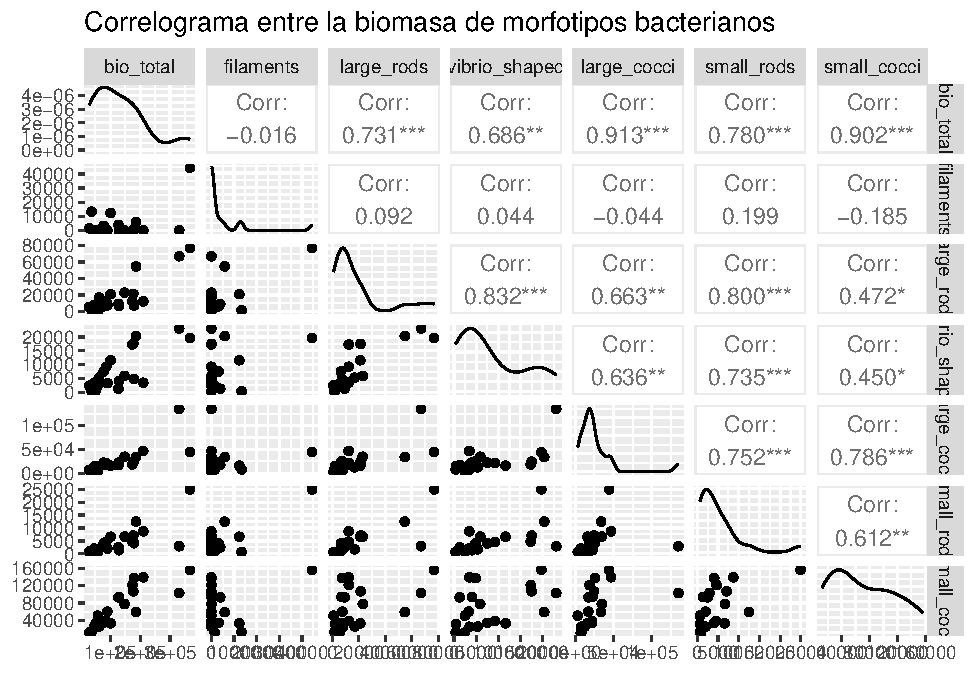
\includegraphics{02-RegMult_files/figure-latex/correlo2-1.pdf}

Ahora visualizaremos la correlación como un mapa de calor.

\begin{Shaded}
\begin{Highlighting}[]
\FunctionTok{ggcorr}\NormalTok{(datos\_bacterias, }\AttributeTok{method =} \FunctionTok{c}\NormalTok{(}\StringTok{"everything"}\NormalTok{, }\StringTok{"pearson"}\NormalTok{)) }
\end{Highlighting}
\end{Shaded}

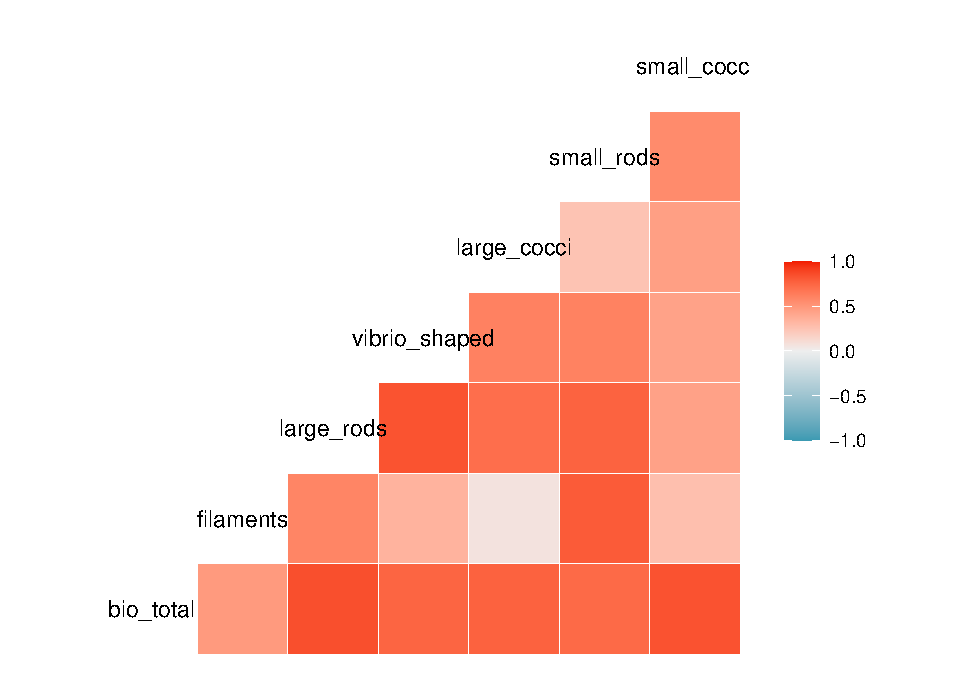
\includegraphics{02-RegMult_files/figure-latex/correlo3-1.pdf}

\begin{Shaded}
\begin{Highlighting}[]
\FunctionTok{ggcorr}\NormalTok{(datos\_bacterias, }\AttributeTok{method =} \FunctionTok{c}\NormalTok{(}\StringTok{"everything"}\NormalTok{, }\StringTok{"spearman"}\NormalTok{)) }
\end{Highlighting}
\end{Shaded}

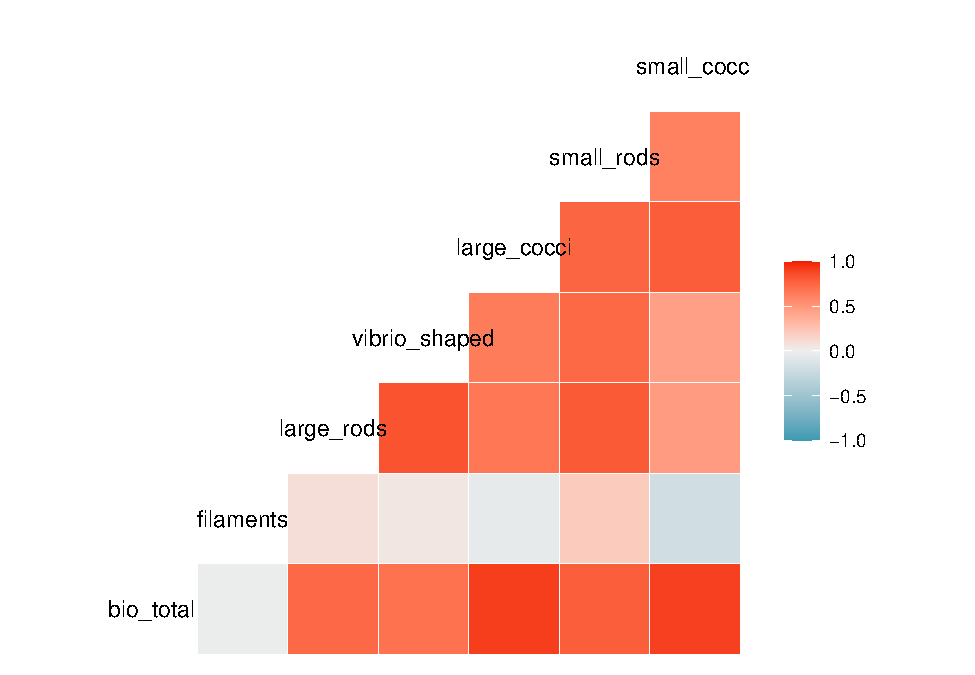
\includegraphics{02-RegMult_files/figure-latex/correlo4-1.pdf}

\hypertarget{entre-variables-abiuxf3ticas}{%
\subsection{Entre variables abióticas}\label{entre-variables-abiuxf3ticas}}

Ahora analizaremos las variables explicativas. Esto es útil ya que en el siguiente paso de realizar regresiones múltiples evitaremos colocar en el modelo dos variables muy correlacionadas entre sí, ya que son redundantes. Generamos un nuevo dataframe que es un subconjunto de los anteriores.

Podemos repetir el estudio de comparar correlaciones de Pearson, de Pearson por permutaciones y de Spearman. Aquí resumidamente pasaremos a los correlogramas visuales. ¿Qué pasa con el oxígeno disuelto? Tendremos cuidado con el uso de esta variable en los análisis siguientes.

\begin{Shaded}
\begin{Highlighting}[]
\NormalTok{datos\_fq }\OtherTok{\textless{}{-}}\NormalTok{ datos\_RH[,}\DecValTok{12}\SpecialCharTok{:}\DecValTok{23}\NormalTok{]}

\FunctionTok{ggcorr}\NormalTok{(datos\_fq, }\AttributeTok{method =} \FunctionTok{c}\NormalTok{(}\StringTok{"everything"}\NormalTok{, }\StringTok{"spearman"}\NormalTok{)) }
\end{Highlighting}
\end{Shaded}

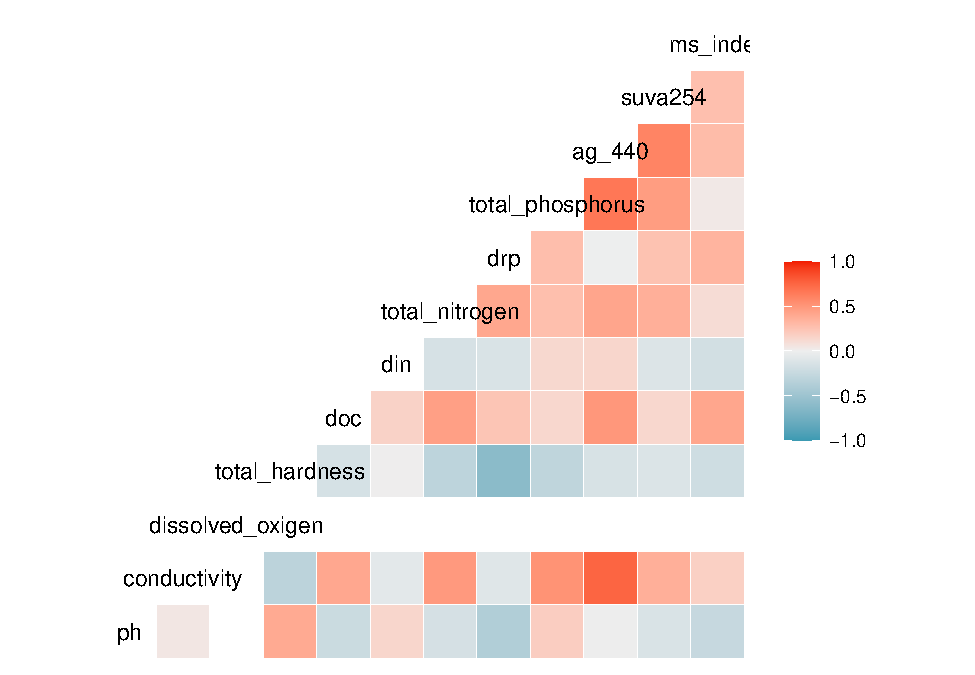
\includegraphics{02-RegMult_files/figure-latex/correlo5-1.pdf}
Si queremos tener un resumen numérico de los coeficientes de correlación, podemos generar una matriz.

\begin{verbatim}
## Warning: package 'Hmisc' was built under R version 4.2.2
\end{verbatim}

\begin{verbatim}
## Loading required package: lattice
\end{verbatim}

\begin{verbatim}
## Loading required package: survival
\end{verbatim}

\begin{verbatim}
## Loading required package: Formula
\end{verbatim}

\begin{verbatim}
## 
## Attaching package: 'Hmisc'
\end{verbatim}

\begin{verbatim}
## The following objects are masked from 'package:dplyr':
## 
##     src, summarize
\end{verbatim}

\begin{verbatim}
## The following objects are masked from 'package:base':
## 
##     format.pval, units
\end{verbatim}

\begin{Shaded}
\begin{Highlighting}[]
\FunctionTok{rcorr}\NormalTok{(}\FunctionTok{as.matrix}\NormalTok{(datos\_fq), }\AttributeTok{type=}\StringTok{"spearman"}\NormalTok{) }
\end{Highlighting}
\end{Shaded}

\begin{verbatim}
##                     ph conductivity dissolved_oxigen total_hardness   doc   din
## ph                1.00         0.05            -0.03           0.39 -0.22  0.14
## conductivity      0.05         1.00             0.06          -0.31  0.41 -0.07
## dissolved_oxigen -0.03         0.06             1.00          -0.34 -0.03 -0.29
## total_hardness    0.39        -0.31            -0.34           1.00 -0.16  0.01
## doc              -0.22         0.41            -0.03          -0.16  1.00  0.16
## din               0.14        -0.07            -0.29           0.01  0.16  1.00
## total_nitrogen   -0.16         0.48            -0.24          -0.30  0.45 -0.15
## drp              -0.38        -0.09            -0.15          -0.60  0.24 -0.13
## total_phosphorus  0.19         0.52            -0.22          -0.29  0.13  0.13
## ag_440           -0.01         0.75            -0.32          -0.14  0.49  0.14
## suva254          -0.13         0.36            -0.63          -0.12  0.13 -0.12
## ms_index         -0.25         0.17            -0.27          -0.20  0.41 -0.18
##                  total_nitrogen   drp total_phosphorus ag_440 suva254 ms_index
## ph                        -0.16 -0.38             0.19  -0.01   -0.13    -0.25
## conductivity               0.48 -0.09             0.52   0.75    0.36     0.17
## dissolved_oxigen          -0.24 -0.15            -0.22  -0.32   -0.63    -0.27
## total_hardness            -0.30 -0.60            -0.29  -0.14   -0.12    -0.20
## doc                        0.45  0.24             0.13   0.49    0.13     0.41
## din                       -0.15 -0.13             0.13   0.14   -0.12    -0.18
## total_nitrogen             1.00  0.41             0.27   0.42    0.36     0.10
## drp                        0.41  1.00             0.28   0.00    0.25     0.33
## total_phosphorus           0.27  0.28             1.00   0.66    0.46     0.03
## ag_440                     0.42  0.00             0.66   1.00    0.59     0.29
## suva254                    0.36  0.25             0.46   0.59    1.00     0.27
## ms_index                   0.10  0.33             0.03   0.29    0.27     1.00
## 
## n
##                  ph conductivity dissolved_oxigen total_hardness doc din
## ph               20           20               15             20  20  20
## conductivity     20           20               15             20  20  20
## dissolved_oxigen 15           15               15             15  15  15
## total_hardness   20           20               15             20  20  20
## doc              20           20               15             20  20  20
## din              20           20               15             20  20  20
## total_nitrogen   20           20               15             20  20  20
## drp              20           20               15             20  20  20
## total_phosphorus 20           20               15             20  20  20
## ag_440           20           20               15             20  20  20
## suva254          20           20               15             20  20  20
## ms_index         20           20               15             20  20  20
##                  total_nitrogen drp total_phosphorus ag_440 suva254 ms_index
## ph                           20  20               20     20      20       20
## conductivity                 20  20               20     20      20       20
## dissolved_oxigen             15  15               15     15      15       15
## total_hardness               20  20               20     20      20       20
## doc                          20  20               20     20      20       20
## din                          20  20               20     20      20       20
## total_nitrogen               20  20               20     20      20       20
## drp                          20  20               20     20      20       20
## total_phosphorus             20  20               20     20      20       20
## ag_440                       20  20               20     20      20       20
## suva254                      20  20               20     20      20       20
## ms_index                     20  20               20     20      20       20
## 
## P
##                  ph     conductivity dissolved_oxigen total_hardness doc   
## ph                      0.8450       0.9094           0.0875         0.3417
## conductivity     0.8450              0.8292           0.1788         0.0760
## dissolved_oxigen 0.9094 0.8292                        0.2182         0.9142
## total_hardness   0.0875 0.1788       0.2182                          0.5120
## doc              0.3417 0.0760       0.9142           0.5120               
## din              0.5541 0.7813       0.2979           0.9824         0.4934
## total_nitrogen   0.5036 0.0318       0.3973           0.1926         0.0472
## drp              0.1009 0.6939       0.5901           0.0048         0.3147
## total_phosphorus 0.4266 0.0192       0.4402           0.2116         0.5765
## ag_440           0.9699 0.0001       0.2474           0.5434         0.0271
## suva254          0.5801 0.1200       0.0126           0.6090         0.5735
## ms_index         0.2850 0.4631       0.3369           0.3975         0.0714
##                  din    total_nitrogen drp    total_phosphorus ag_440 suva254
## ph               0.5541 0.5036         0.1009 0.4266           0.9699 0.5801 
## conductivity     0.7813 0.0318         0.6939 0.0192           0.0001 0.1200 
## dissolved_oxigen 0.2979 0.3973         0.5901 0.4402           0.2474 0.0126 
## total_hardness   0.9824 0.1926         0.0048 0.2116           0.5434 0.6090 
## doc              0.4934 0.0472         0.3147 0.5765           0.0271 0.5735 
## din                     0.5348         0.5760 0.5876           0.5560 0.6267 
## total_nitrogen   0.5348                0.0740 0.2464           0.0675 0.1193 
## drp              0.5760 0.0740                0.2333           0.9873 0.2787 
## total_phosphorus 0.5876 0.2464         0.2333                  0.0015 0.0393 
## ag_440           0.5560 0.0675         0.9873 0.0015                  0.0057 
## suva254          0.6267 0.1193         0.2787 0.0393           0.0057        
## ms_index         0.4556 0.6686         0.1489 0.8907           0.2144 0.2494 
##                  ms_index
## ph               0.2850  
## conductivity     0.4631  
## dissolved_oxigen 0.3369  
## total_hardness   0.3975  
## doc              0.0714  
## din              0.4556  
## total_nitrogen   0.6686  
## drp              0.1489  
## total_phosphorus 0.8907  
## ag_440           0.2144  
## suva254          0.2494  
## ms_index
\end{verbatim}

\hypertarget{regresiones-muxfaltiples}{%
\section{Regresiones múltiples}\label{regresiones-muxfaltiples}}

Intro

hay que estandarizar?

\hypertarget{selecciuxf3n-automuxe1tica-de-variables}{%
\subsection{Selección automática de variables}\label{selecciuxf3n-automuxe1tica-de-variables}}

\hypertarget{upward-del-modelo-nulo-sumando-variables-explicativas}{%
\subsubsection{Upward: del modelo nulo, sumando variables explicativas}\label{upward-del-modelo-nulo-sumando-variables-explicativas}}

\hypertarget{forward-del-modelo-completo-quitando-variables-explicativas}{%
\subsubsection{Forward: del modelo completo, quitando variables explicativas}\label{forward-del-modelo-completo-quitando-variables-explicativas}}

\hypertarget{selecciuxf3n-manual-de-variables}{%
\subsection{Selección manual de variables}\label{selecciuxf3n-manual-de-variables}}

\hypertarget{modelos-univariados}{%
\subsubsection{Modelos univariados}\label{modelos-univariados}}

Todos los modelos
AIC

\hypertarget{modelos-de-regresiuxf3n-muxfaltiple}{%
\subsubsection{Modelos de regresión múltiple}\label{modelos-de-regresiuxf3n-muxfaltiple}}

vif

\hypertarget{evaluaciuxf3n-e-interpretaciuxf3n-del-modelo-final}{%
\subsection{Evaluación e interpretación del modelo final}\label{evaluaciuxf3n-e-interpretaciuxf3n-del-modelo-final}}

Evaluación de supuestos. Si no se cumplen, permutaciones
interpretación

\hypertarget{a-modo-de-conclusiuxf3n}{%
\section{A modo de conclusión}\label{a-modo-de-conclusiuxf3n}}

\hypertarget{gam}{%
\chapter{Modelos Aditivos Generalizados}\label{gam}}

\textbf{María Victoria Quiroga}\footnote{\href{mailto:mvquiroga@iib.unsam.edu.ar}{\nolinkurl{mvquiroga@iib.unsam.edu.ar}}}

Instituto Tecnológico de Chascomús (INTECH, UNSAM-CONICET), Escuela de Bio y Nanotecnologías (UNSAM)

\hypertarget{aclaraciuxf3n}{%
\subsection{Aclaración}\label{aclaraciuxf3n}}

En esta unidad se utiliza el paquete \emph{ggplot2} \citep{ggplot2} para generar algunos gráficos. Para comprender el código empleado se recomienda leer el \emph{Capítulo 3: Data visualization} del libro \emph{R for Data Science} \citep{wickham2017r}.

\hypertarget{porquuxe9-usar-modelos-aditivos-generalizados-gams}{%
\section{¿Porqué usar Modelos Aditivos Generalizados (GAMs)?}\label{porquuxe9-usar-modelos-aditivos-generalizados-gams}}

\begin{enumerate}
\def\labelenumi{\arabic{enumi}.}
\tightlist
\item
  La relación entre variables predictoras (i.e., independientes) y la variable respuesta (i.e., dependiente) \textbf{no} necesita ser \textbf{lineal}.
\item
  \textbf{No} necesitamos conocer de antemano la forma funcional de la relación.
\item
  Son modelos muy flexibles que permiten la interpretación (de manera gráfica) de los efectos parciales de cada variable independiente.
\item
  Podemos:
\end{enumerate}

\begin{itemize}
\tightlist
\item
  Incluir predictores categóricos e interacciones.
\item
  Usar distribuciones diferentes a la normal para la variable dependiente.
\item
  Incluir correlaciones entre observaciones (e.g., medidas repetidas, diseños anidados) -modelos mixtos.
\end{itemize}

\hypertarget{quuxe9-son-los-gams}{%
\section{¿Qué son los GAMs?}\label{quuxe9-son-los-gams}}

Los GAM permiten incorporar los efectos additivos de distintas variables independientes (i.e., explicativas) utilizando funciones suaves (\(smooth functions\)).

\[
g(\mu) = \beta_0 + f_{1}(x_{1}) + f_{2}(x_{2}) + ... + f_{n}(x_{n}) + \varepsilon
\]

Donde \(\mu\) es el valor esperado de la variable dependiente \emph{y} que puede presentar distribuciones de la familia exponencial, \emph{g} es la función de enlace, \(\beta_0\) es el intercepto, \(x_{n}\) son las \emph{n} variables independientes y cada \(f_{n}\) es una función suave que se estima de manera no paramétrica. Se pueden incluir funciones suaves para interacciones, por ejemplo entre las variables independientes 1 y 2 \(f(x_{1},x_{2})\). Si se incluyen términos aditivos aleatorios, por ejemplo la autocorrelación en series de tiempo, se generan modelos mixtos (GAMM, \emph{generalized additive mixed model}).

Existen diferentes estrategias para ajustar una curva suave y continua a los datos. Aquí vamos a utilizar \emph{splines}, y en particular \emph{spline} cúbico y cúbico cíclico. De manera muy breve, un \emph{spline} cúbico es una curva suave cúbica por tramos (Figura \ref{fig:Splines}). El \emph{spline} cúbico cíclico empieza y termina en el mismo punto. El paquete con el que vamos a trabajar \emph{mgcv} \citep{wood2017} usa splines penalizados ( \emph{conventional intergrated square second derivative cubic spline penalty}), donde la penalización será más grande cuanto menos suave sea la curva.

\begin{figure}

{\centering 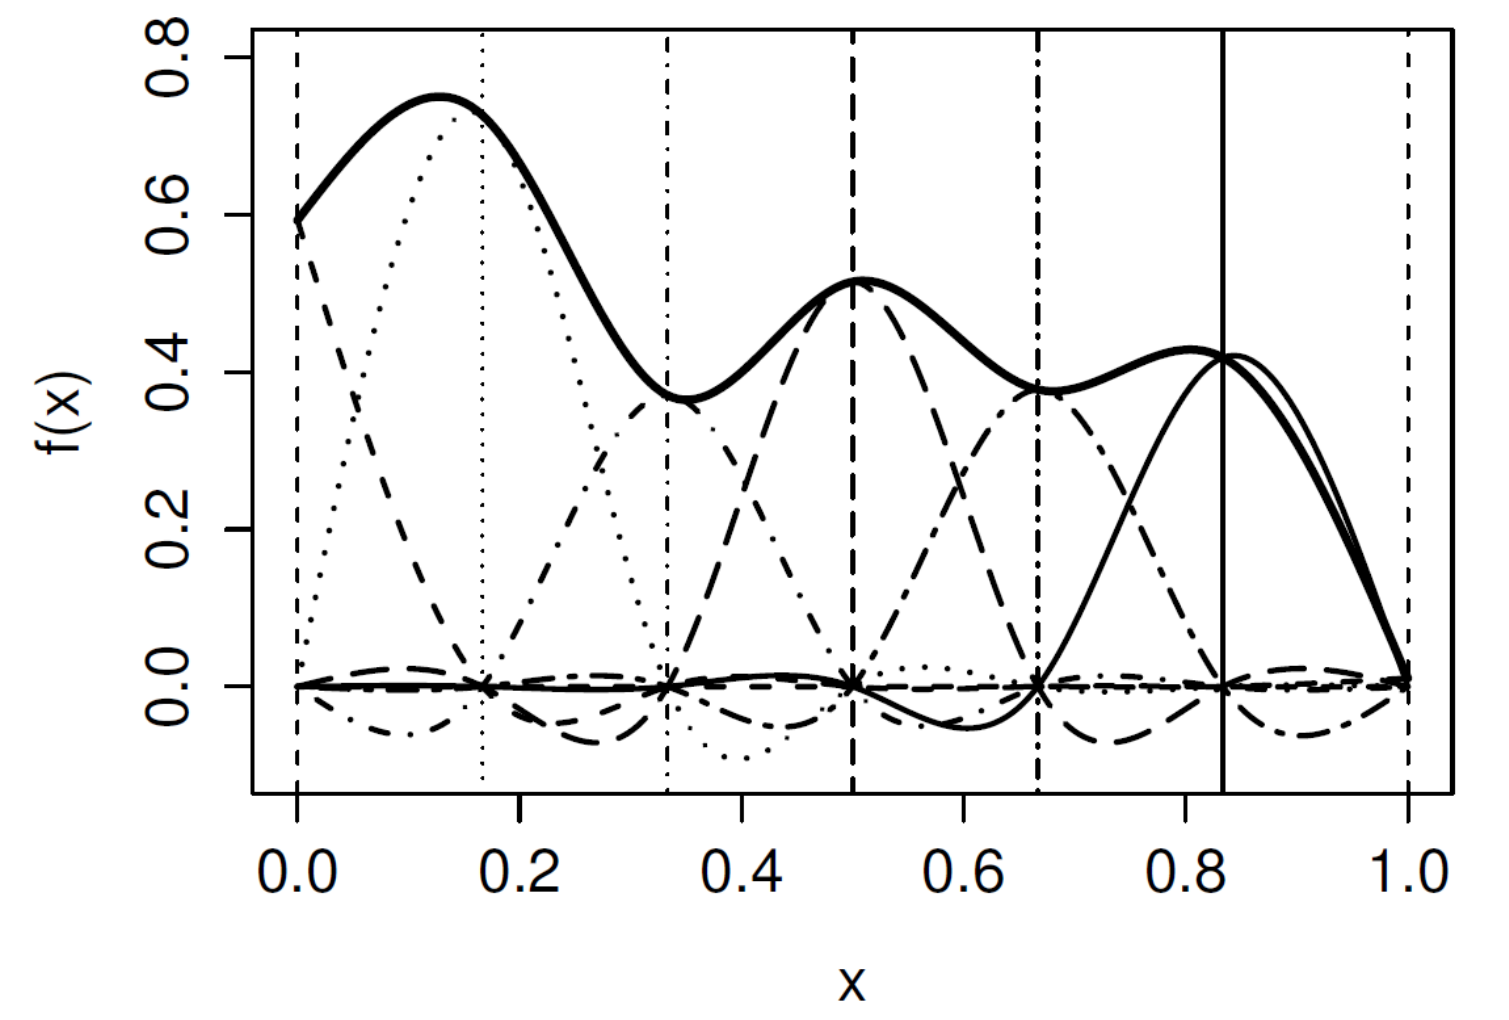
\includegraphics[width=0.8\linewidth]{./images/Splines} 

}

\caption{Construcción de un spline cúbico. La curva suave (línea contínua gruesa) es la suma de las 5 funciones basis (líneas finas). Las líneas verticales muestran los nodos equiespaciados. Extraído de Wood (2017).}\label{fig:Splines}
\end{figure}

\hypertarget{manos-a-la-obra}{%
\section{Manos a la obra!}\label{manos-a-la-obra}}

Utilizaremos un set de datos del trabajo \emph{The dynamics of picocyanobacteria from a hypereutrophic shallow lake is affected by light-climate and small-bodied zooplankton: a 10-year cytometric time-series analysis} publicado en \emph{FEMS Microbiology Ecology} \citep{quiroga2021}, disponibles en el \href{http://hdl.handle.net/11336/200094}{Repositorio Institucional CONICET Digital}.

Descargar el set de datos \textbf{data\_gam.csv} de \href{https://github.com/Limno-con-R/CILCAL2023/tree/main/datasets}{GitHub Limno-con-R/CILCAL2023}.
Guardar el archivo en una carpeta llamada \emph{data}, dentro del \textbf{Directorio de Trabajo} del \textbf{Proyecto} que creamos para esta Unidad (ver cómo hacerlo en la Unidad \ref{intro}).

Instalar los paquetes como se indica en la Unidad \ref{intro}. Luego, cargarlos en la sesión

\begin{Shaded}
\begin{Highlighting}[]
\FunctionTok{library}\NormalTok{(mgcv)}
\FunctionTok{library}\NormalTok{(ggplot2)}
\FunctionTok{library}\NormalTok{(itsadug)}
\FunctionTok{library}\NormalTok{(data.table)}
\FunctionTok{library}\NormalTok{(car)}
\FunctionTok{library}\NormalTok{(grid)}
\FunctionTok{library}\NormalTok{(lubridate)}
\end{Highlighting}
\end{Shaded}

Leer datos, dar formato \texttt{as.Date} a la fecha y generar las variables \texttt{Mes} y \texttt{Dias}.

\begin{Shaded}
\begin{Highlighting}[]
\NormalTok{base }\OtherTok{\textless{}{-}} \FunctionTok{read.csv}\NormalTok{(}\StringTok{"data/data\_gam.csv"}\NormalTok{)}
\NormalTok{base}\SpecialCharTok{$}\NormalTok{Fecha }\OtherTok{\textless{}{-}} \FunctionTok{as.Date}\NormalTok{(base}\SpecialCharTok{$}\NormalTok{Fecha, }\StringTok{"\%m/\%d/\%Y"}\NormalTok{) }\CommentTok{\# formato de fecha en inglés}
\NormalTok{base}\SpecialCharTok{$}\NormalTok{Mes }\OtherTok{\textless{}{-}} \FunctionTok{as.numeric}\NormalTok{(}\FunctionTok{format}\NormalTok{(base}\SpecialCharTok{$}\NormalTok{Fecha,}\StringTok{\textquotesingle{}\%m\textquotesingle{}}\NormalTok{)) }\CommentTok{\# generar variable Mes}
\NormalTok{base}\SpecialCharTok{$}\NormalTok{Dia1 }\OtherTok{=} \FunctionTok{rep}\NormalTok{(base}\SpecialCharTok{$}\NormalTok{Fecha[}\DecValTok{1}\NormalTok{], }\FunctionTok{nrow}\NormalTok{(base)) }\CommentTok{\# fecha inicial de la serie}
\NormalTok{base}\SpecialCharTok{$}\NormalTok{Dias }\OtherTok{\textless{}{-}}\NormalTok{ (}\FunctionTok{interval}\NormalTok{(base}\SpecialCharTok{$}\NormalTok{Dia1, base}\SpecialCharTok{$}\NormalTok{Fecha) }\SpecialCharTok{\%/\%} \FunctionTok{days}\NormalTok{(}\DecValTok{1}\NormalTok{))}\SpecialCharTok{+}\DecValTok{1} \CommentTok{\# generar variable Dias}
\end{Highlighting}
\end{Shaded}

Inspección visual de primeras filas de la tabla. Para ver toda la tabla se puede utilizar \texttt{View(base)}.

\begin{Shaded}
\begin{Highlighting}[]
\FunctionTok{head}\NormalTok{(base)}
\end{Highlighting}
\end{Shaded}

\begin{verbatim}
##        Fecha Pcy_orgml Mes       Dia1 Dias
## 1 2007-05-22   6660000   5 2007-05-22    1
## 2 2007-06-05   6830000   6 2007-05-22   15
## 3 2007-06-21   4700000   6 2007-05-22   31
## 4 2007-07-03   4680000   7 2007-05-22   43
## 5 2007-07-17   6500000   7 2007-05-22   57
## 6 2007-07-31   8110000   7 2007-05-22   71
\end{verbatim}

Ver la estructura de los datos

\begin{Shaded}
\begin{Highlighting}[]
\FunctionTok{str}\NormalTok{(base)}
\end{Highlighting}
\end{Shaded}

\begin{verbatim}
## 'data.frame':    225 obs. of  5 variables:
##  $ Fecha    : Date, format: "2007-05-22" "2007-06-05" ...
##  $ Pcy_orgml: num  6660000 6830000 4700000 4680000 6500000 8110000 8840000 11000000 10100000 6340000 ...
##  $ Mes      : num  5 6 6 7 7 7 8 8 9 9 ...
##  $ Dia1     : Date, format: "2007-05-22" "2007-05-22" ...
##  $ Dias     : num  1 15 31 43 57 71 85 99 113 127 ...
\end{verbatim}

\texttt{base} es un objeto \texttt{data.frame} con 225 \texttt{obs.} observaciones o filas y 5 \texttt{variables} o columnas.
Variables: \texttt{Fecha} con formato \texttt{Date}. \texttt{Pcy\_orgml}, abundancia de picocianobacterias (organismos/ml) en la laguna Chascomús, como valores numéricos \texttt{num}.

Se generaron las variables \texttt{Mes} y \texttt{Dias} como números \texttt{num}. \texttt{Mes} indica el \#mes (1-12) de la fecha de muestreo y \texttt{Dias} indica el \#días transcurridos desde la primer fecha (considerando la primer fecha como día \#1).

Grafico exploratorio de la serie temporal

\begin{Shaded}
\begin{Highlighting}[]
\FunctionTok{ggplot}\NormalTok{(base, }\FunctionTok{aes}\NormalTok{(}\AttributeTok{x=}\NormalTok{ Dias, }\AttributeTok{y=}\NormalTok{ Pcy\_orgml))  }\SpecialCharTok{+}
  \FunctionTok{geom\_point}\NormalTok{()  }\SpecialCharTok{+}
  \FunctionTok{geom\_line}\NormalTok{()}\SpecialCharTok{+}
  \FunctionTok{theme}\NormalTok{(}\AttributeTok{legend.position =} \StringTok{"none"}\NormalTok{)}
\end{Highlighting}
\end{Shaded}

\begin{figure}

{\centering 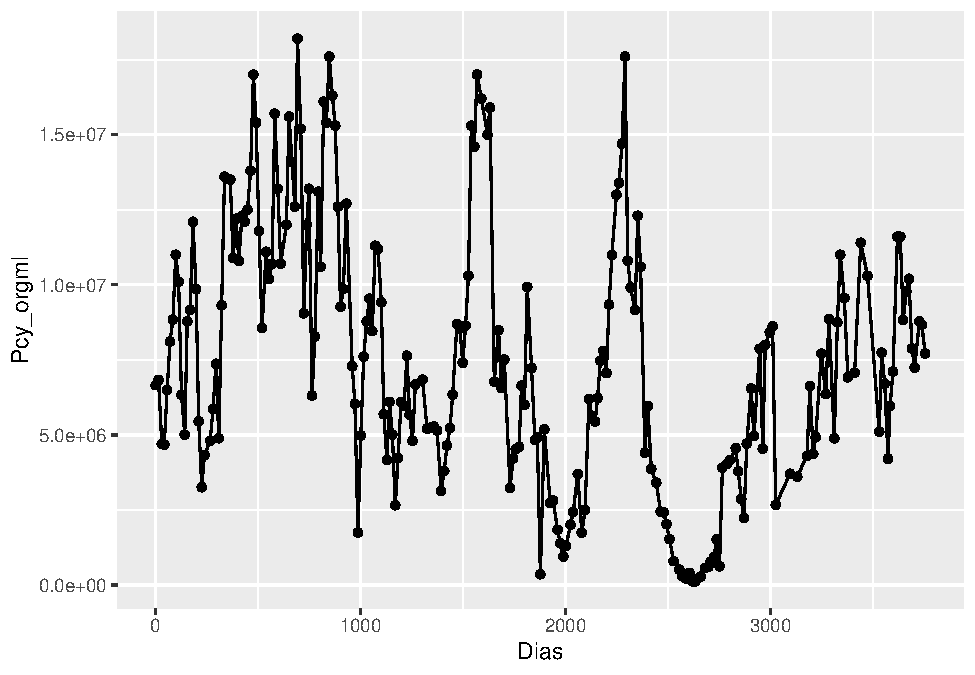
\includegraphics[width=0.8\linewidth]{03-gam_files/figure-latex/serie-1} 

}

\caption{Serie temporal de abundancia (organismos/ml) de picocianobacterias.}\label{fig:serie}
\end{figure}

No se observan outliers en el gráfico.

Para datos de conteo (e.g., organismos/ml) generalmente se utiliza la distribución de Poisson, pero las series temporales de abundancia de microorganismos suelen presentar sobredispersión (Figura \ref{fig:serie}). Para considerar una varianza mayor que la media se podría utilizar la distribución binomial negativa o la \emph{quasi-familia} quasipoisson. En este ejemplo se implementará \texttt{family=quasipoisson}.

La autocorrelación temporal de los datos se incluye utilizando una estructura autorregresiva de primer orden continua \texttt{correlation\ =\ corCAR1(form\ =\ \textasciitilde{}\ Dias)} en un modelo mixto \texttt{gamm()}.

Como primer modelado se generan funciones suaves \texttt{s()} para el efecto estacional \texttt{Mes} y el efecto interanual ( \emph{trend}) \texttt{Dias}. Se utiliza \emph{spline} cúbico cíclico para el primer efecto \texttt{s(Mes,\ bs="cc")} y cúbico para el segundo efecto \texttt{s(Dias,\ bs="cr")}.

\begin{Shaded}
\begin{Highlighting}[]
\NormalTok{modelo1}\OtherTok{\textless{}{-}}\FunctionTok{gamm}\NormalTok{(Pcy\_orgml }\SpecialCharTok{\textasciitilde{}} \FunctionTok{s}\NormalTok{(Mes, }\AttributeTok{bs =} \StringTok{"cc"}\NormalTok{) }\SpecialCharTok{+} \FunctionTok{s}\NormalTok{(Dias, }\AttributeTok{bs=}\StringTok{"cr"}\NormalTok{), }
              \AttributeTok{family=}\NormalTok{quasipoisson, }\AttributeTok{data =}\NormalTok{ base, }
              \AttributeTok{correlation =} \FunctionTok{corCAR1}\NormalTok{(}\AttributeTok{form =} \SpecialCharTok{\textasciitilde{}}\NormalTok{ Dias))}
\end{Highlighting}
\end{Shaded}

\begin{verbatim}
## 
##  Maximum number of PQL iterations:  20
\end{verbatim}

\begin{verbatim}
## iteration 1
\end{verbatim}

\begin{verbatim}
## iteration 2
\end{verbatim}

\begin{verbatim}
## iteration 3
\end{verbatim}

\begin{verbatim}
## iteration 4
\end{verbatim}

Por \emph{default} el máximo número de iteraciones está seteado en 20 \texttt{niterPQL=20}. Si el modelo no converge se puede incrementar el número de interacciones, por ejemplo: \texttt{gamm(...,\ niterPQL=40)}.

Interpretación visual de los efectos parciales: curvas suaves \texttt{s()} ( \emph{smooth functions})

\begin{Shaded}
\begin{Highlighting}[]
\FunctionTok{plot}\NormalTok{(modelo1}\SpecialCharTok{$}\NormalTok{gam, }\AttributeTok{scale=}\DecValTok{0}\NormalTok{, }\AttributeTok{scheme=}\DecValTok{1}\NormalTok{, }\AttributeTok{pages=}\DecValTok{1}\NormalTok{)}
\end{Highlighting}
\end{Shaded}

\textbackslash begin\{figure\}

\{\centering 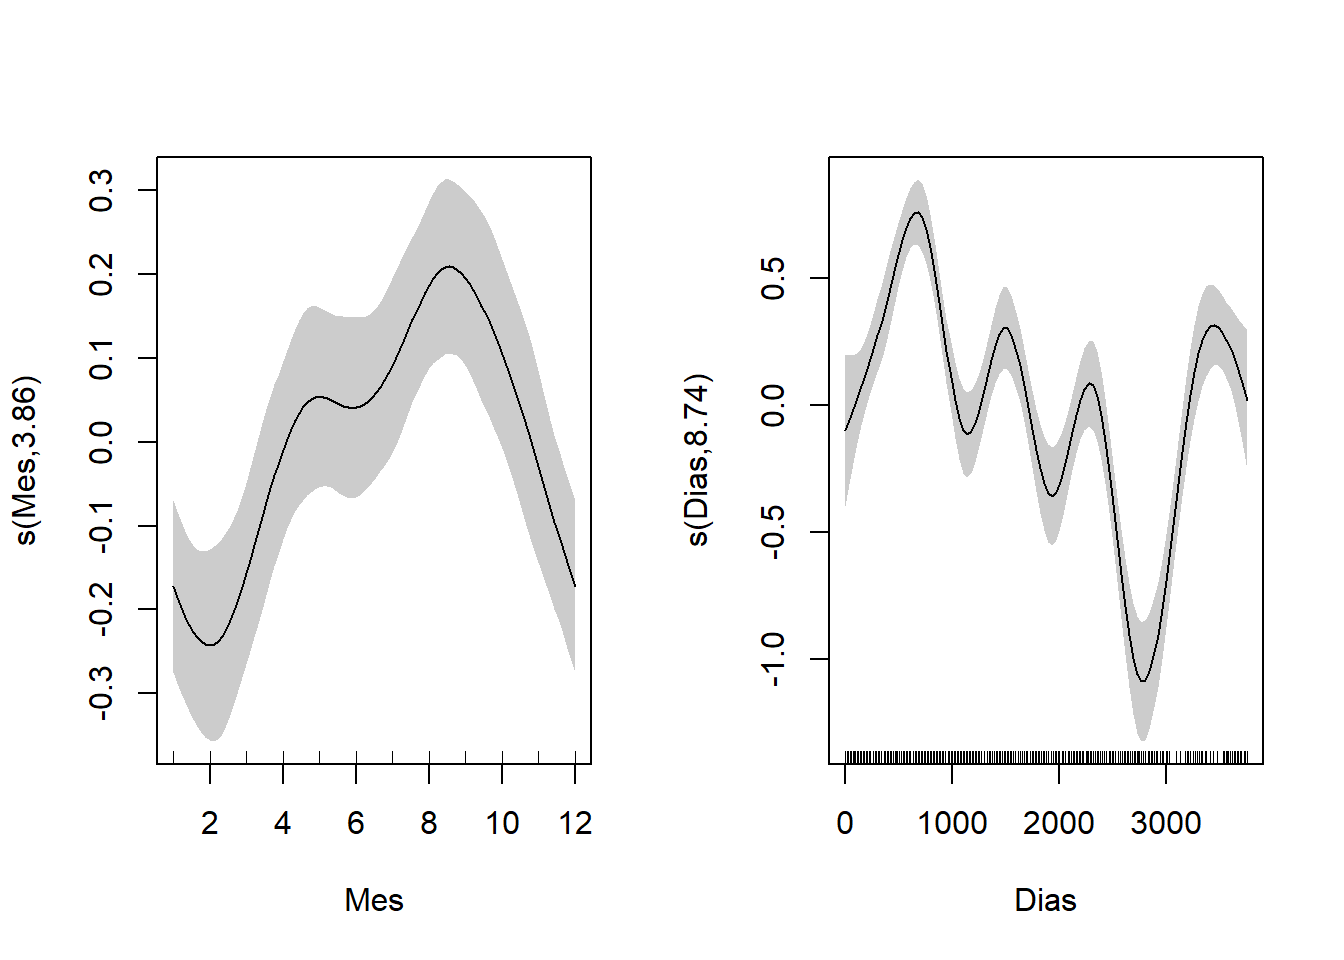
\includegraphics[width=1\linewidth]{03-gam_files/figure-latex/unnamed-chunk-6-1}

\}

\textbackslash caption\{Efectos parciales del modelo 1. Las curvas suaves se centraron en cero, se indican los intervalos de confianza de 95\% en gris. Las líneas internas en los ejes x (Mes y Dias) representan los datos.\}\label{fig:unnamed-chunk-6}
\textbackslash end\{figure\}

Información del modelo

\begin{Shaded}
\begin{Highlighting}[]
\FunctionTok{summary}\NormalTok{(modelo1}\SpecialCharTok{$}\NormalTok{gam)}
\end{Highlighting}
\end{Shaded}

\begin{verbatim}
## 
## Family: quasipoisson 
## Link function: log 
## 
## Formula:
## Pcy_orgml ~ s(Mes, bs = "cc") + s(Dias, bs = "cr")
## 
## Parametric coefficients:
##             Estimate Std. Error t value Pr(>|t|)    
## (Intercept) 15.72716    0.02977   528.2   <2e-16 ***
## ---
## Signif. codes:  0 '***' 0.001 '**' 0.01 '*' 0.05 '.' 0.1 ' ' 1
## 
## Approximate significance of smooth terms:
##           edf Ref.df      F  p-value    
## s(Mes)  3.858  8.000  3.674 3.46e-06 ***
## s(Dias) 8.743  8.743 23.752  < 2e-16 ***
## ---
## Signif. codes:  0 '***' 0.001 '**' 0.01 '*' 0.05 '.' 0.1 ' ' 1
## 
## R-sq.(adj) =  0.564   
##   Scale est. = 1.209e+06  n = 225
\end{verbatim}

Se especifica la familia que se utilizó \texttt{\#\#\ Family:\ quasipoisson} y la función de enlace \texttt{\#\#\ Link\ function:\ log}. \texttt{?family} muestra las familias y funciones de enlace que se utilizan por \emph{default}. Para cambiar la función de enlace solo hay que especificarlo en el código, ejemplo \texttt{family\ =\ Gamma(link\ =\ "log")}. Si no se especifica una familia, \texttt{gamm} usa distribución gaussiana con función de enlace identidad. La ayuda \texttt{?gamm} muestra todos los argumentos y los \emph{defaults}.

Se observa que ambos términos de suavizado son significativos (\texttt{p-value} \textless{} 0.05), y el \(R_{adj}^{2}\) del modelo es 0.5640034.

Evaluación del modelo

\begin{Shaded}
\begin{Highlighting}[]
\FunctionTok{windows}\NormalTok{()}
\FunctionTok{par}\NormalTok{(}\AttributeTok{mfrow=}\FunctionTok{c}\NormalTok{(}\DecValTok{2}\NormalTok{,}\DecValTok{2}\NormalTok{))}
\FunctionTok{gam.check}\NormalTok{(modelo1}\SpecialCharTok{$}\NormalTok{gam, }\AttributeTok{type=}\StringTok{"pearson"}\NormalTok{)}
\end{Highlighting}
\end{Shaded}

\begin{figure}

{\centering 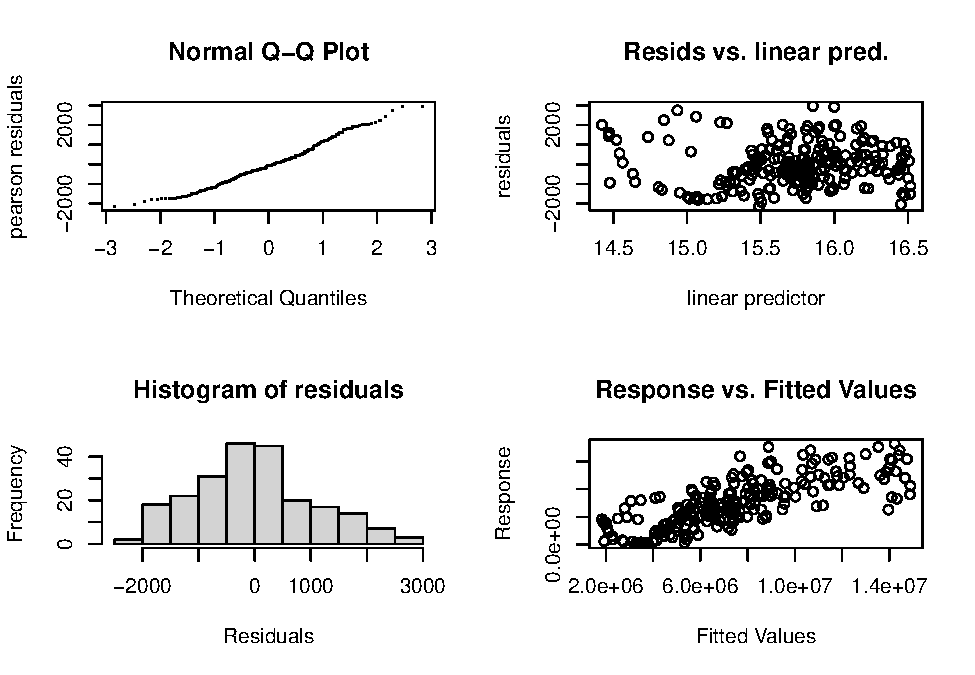
\includegraphics[width=1\linewidth]{03-gam_files/figure-latex/check-1} 

}

\caption{gam.check del modelo 1.}\label{fig:check}
\end{figure}

\begin{verbatim}
## 
## 'gamm' based fit - care required with interpretation.
## Checks based on working residuals may be misleading.
## Basis dimension (k) checking results. Low p-value (k-index<1) may
## indicate that k is too low, especially if edf is close to k'.
## 
##           k'  edf k-index p-value    
## s(Mes)  8.00 3.86    0.93    0.14    
## s(Dias) 9.00 8.74    0.31  <2e-16 ***
## ---
## Signif. codes:  0 '***' 0.001 '**' 0.01 '*' 0.05 '.' 0.1 ' ' 1
\end{verbatim}

Los gráficos de la izquierda de la Figura \ref{fig:check} muestran que es correcto utilizar la \emph{quasi familia} quasipoisson. El gráfico superior derecho muestra una dispersión bastante homogénea de los residuos, por lo que no habría mayores problemas con la varianza. El gráfico inferior derecho muestra una relación lineal positiva entre los valores observados y los predichos por el modelo. Si se logra mejorar el modelo, se observará una mejoría en este gráfico y en el \(R_{adj}^{2}\) del modelo.

En el modelo 1 no se especificó el \texttt{k} en los términos de suavizado \texttt{s()}, se utilizó la opción \emph{default} \texttt{k\ =\ 10}. Este argumento especifica la dimensión de las funciones \emph{basis} del \emph{spline}. Cuando se indica un valor de \texttt{k}, este determina el máximo grado de libertad permitida para ese término del modelo. Sin embargo, los grados de libertad efectivos \texttt{edf} para cada término los estima el modelo a través de la penalización, siendo el límite superior \(k' = k - 1\). No especificar el argumento \texttt{k} equivale a indicar \texttt{k\ =\ 10}.

El \texttt{gam.check()} nos indica que el \texttt{k} del término \texttt{s(Dias)} del modelo 1 es muy bajo (valor de \texttt{p-value} bajo y \texttt{edf} cercano a \texttt{k\textquotesingle{}}. Ver \texttt{?choose.k} para mas detalles.

Para mejorar el modelo se modifica \texttt{k}. Se disminuye \texttt{k\ =\ 6} en \texttt{s(Mes)} para evitar que incrementen los \texttt{edf} de ese término, y se aumenta \texttt{k\ =\ 20} en \texttt{s(Dias)}. Además, se agrega un término de interacción \texttt{ti()} adecuando para trabajar con variables que tienen diferentes unidades (meses \emph{versus} días).

\begin{Shaded}
\begin{Highlighting}[]
\NormalTok{modelo2}\OtherTok{\textless{}{-}}\FunctionTok{gamm}\NormalTok{(Pcy\_orgml }\SpecialCharTok{\textasciitilde{}} \FunctionTok{s}\NormalTok{(Mes, }\AttributeTok{bs =} \StringTok{"cc"}\NormalTok{, }\AttributeTok{k=}\DecValTok{6}\NormalTok{) }\SpecialCharTok{+} \FunctionTok{s}\NormalTok{(Dias, }\AttributeTok{bs=}\StringTok{"cr"}\NormalTok{, }\AttributeTok{k=}\DecValTok{20}\NormalTok{) }
              \SpecialCharTok{+} \FunctionTok{ti}\NormalTok{(Mes,Dias, }\AttributeTok{bs=}\FunctionTok{c}\NormalTok{(}\StringTok{"cc"}\NormalTok{,}\StringTok{"cr"}\NormalTok{)), }\AttributeTok{family=}\NormalTok{quasipoisson, }
              \AttributeTok{data =}\NormalTok{ base, }\AttributeTok{correlation =} \FunctionTok{corCAR1}\NormalTok{(}\AttributeTok{form =} \SpecialCharTok{\textasciitilde{}}\NormalTok{ Dias))}
\end{Highlighting}
\end{Shaded}

\begin{verbatim}
## 
##  Maximum number of PQL iterations:  20
\end{verbatim}

\begin{verbatim}
## iteration 1
\end{verbatim}

\begin{verbatim}
## iteration 2
\end{verbatim}

\begin{verbatim}
## iteration 3
\end{verbatim}

Interpretación visual de los efectos parciales: curvas suaves \texttt{s()}( \emph{smooth functions})

\begin{Shaded}
\begin{Highlighting}[]
\FunctionTok{plot}\NormalTok{(modelo2}\SpecialCharTok{$}\NormalTok{gam, }\AttributeTok{scale=}\DecValTok{0}\NormalTok{, }\AttributeTok{scheme=}\DecValTok{1}\NormalTok{, }\AttributeTok{pages=}\DecValTok{1}\NormalTok{)}
\end{Highlighting}
\end{Shaded}

\textbackslash begin\{figure\}

\{\centering \includegraphics[width=1\linewidth]{03-gam_files/figure-latex/unnamed-chunk-9-1}

\}

\textbackslash caption\{Efectos parciales del modelo 2. Las curvas suaves se centraron en cero, se indican los intervalos de confianza de 95\% en gris. Las líneas internas en los ejes x (Mes y Dias) representan los datos.\}\label{fig:unnamed-chunk-9}
\textbackslash end\{figure\}

La interacción se muestra en 3D, y es difícil de interpretar visualmente. Aquí nos centramos en la interpretación visual de los efectos parciales.

Información del nuevo modelo

\begin{Shaded}
\begin{Highlighting}[]
\FunctionTok{summary}\NormalTok{(modelo2}\SpecialCharTok{$}\NormalTok{gam)}
\end{Highlighting}
\end{Shaded}

\begin{verbatim}
## 
## Family: quasipoisson 
## Link function: log 
## 
## Formula:
## Pcy_orgml ~ s(Mes, bs = "cc", k = 6) + s(Dias, bs = "cr", k = 20) + 
##     ti(Mes, Dias, bs = c("cc", "cr"))
## 
## Parametric coefficients:
##             Estimate Std. Error t value Pr(>|t|)    
## (Intercept) 15.64156    0.02398   652.3   <2e-16 ***
## ---
## Signif. codes:  0 '***' 0.001 '**' 0.01 '*' 0.05 '.' 0.1 ' ' 1
## 
## Approximate significance of smooth terms:
##                 edf Ref.df      F p-value    
## s(Mes)        3.268   4.00  9.085  <2e-16 ***
## s(Dias)      17.539  17.54 28.940  <2e-16 ***
## ti(Mes,Dias)  3.718  12.00  0.595  0.0395 *  
## ---
## Signif. codes:  0 '***' 0.001 '**' 0.01 '*' 0.05 '.' 0.1 ' ' 1
## 
## R-sq.(adj) =  0.753   
##   Scale est. = 5.8774e+05  n = 225
\end{verbatim}

Los efectos parciales de \texttt{s(Mes)} y \texttt{s(Dias)} son significativos, y la interacción \texttt{ti(Mes,Dias)} es significativa. El \(R_{adj}^{2}\) del modelo aumentó a 0.7532274.

Evaluación del modelo

\begin{Shaded}
\begin{Highlighting}[]
\FunctionTok{windows}\NormalTok{()}
\FunctionTok{par}\NormalTok{(}\AttributeTok{mfrow=}\FunctionTok{c}\NormalTok{(}\DecValTok{2}\NormalTok{,}\DecValTok{2}\NormalTok{))}
\FunctionTok{gam.check}\NormalTok{(modelo2}\SpecialCharTok{$}\NormalTok{gam, }\AttributeTok{type=}\StringTok{"pearson"}\NormalTok{)}
\end{Highlighting}
\end{Shaded}

\begin{figure}

{\centering 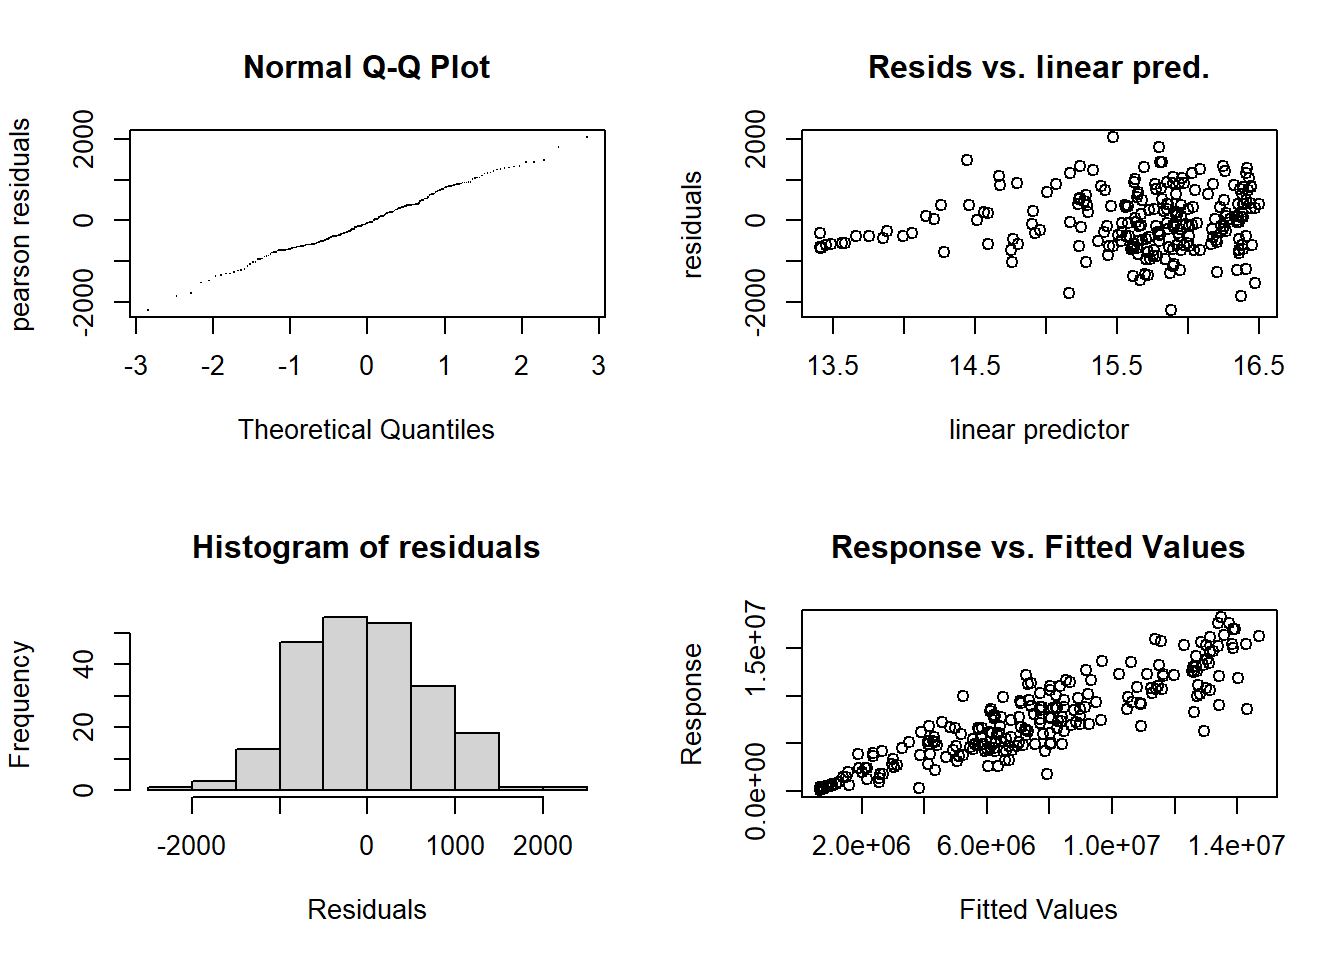
\includegraphics[width=1\linewidth]{03-gam_files/figure-latex/check2-1} 

}

\caption{gam.check del modelo 2.}\label{fig:check2}
\end{figure}

\begin{verbatim}
## 
## 'gamm' based fit - care required with interpretation.
## Checks based on working residuals may be misleading.
## Basis dimension (k) checking results. Low p-value (k-index<1) may
## indicate that k is too low, especially if edf is close to k'.
## 
##                 k'   edf k-index p-value    
## s(Mes)        4.00  3.27    0.84   0.005 ** 
## s(Dias)      19.00 17.54    0.66  <2e-16 ***
## ti(Mes,Dias) 12.00  3.72    0.89   0.010 ** 
## ---
## Signif. codes:  0 '***' 0.001 '**' 0.01 '*' 0.05 '.' 0.1 ' ' 1
\end{verbatim}

De nuevo, parece correcto utilizar la \emph{quasi familia} quasipoisson, sin mayores problemas con la varianza. La relación lineal positiva entre los valores observados y los predichos (gráfico inferior derecho) ha mejorado, coincidiendo con el incremento del \(R_{adj}^{2}\) del modelo.

Los \texttt{edf} del término \texttt{s(Mes)} son cercanos a 3, muy similares al primer modelo, lo cual corrobora que la especificación de k en el modelo no es crítica (modelo 1 \texttt{k\ =\ 10}, modelo 2 \texttt{k\ =\ 6}), siempre que se considere un límite superior adecuado. Para \texttt{s(Dias)} el p-value sigue siendo bajo y \texttt{edf} sigue cercano a \texttt{k\textquotesingle{}}, pero \texttt{k-index} aumentó a 0.66. Se considera que no es necesario aumentar el \texttt{k} porque complejizaría el modelo, y consecuentemente la interpretación visual de la tendencia ( \emph{trend}, efecto Dias).

Se pueden comparar ambos modelos estimando su AIC

\begin{Shaded}
\begin{Highlighting}[]
\FunctionTok{AIC}\NormalTok{(modelo1}\SpecialCharTok{$}\NormalTok{lme,modelo2}\SpecialCharTok{$}\NormalTok{lme)}
\end{Highlighting}
\end{Shaded}

\begin{verbatim}
##             df      AIC
## modelo1$lme  6 311.8362
## modelo2$lme  8 228.2012
\end{verbatim}

Efectivamente el modelo 2 presenta un AIC más bajo.

\textbf{Otros gráficos}

Se puede graficar con \texttt{vis.gam()}.

\begin{Shaded}
\begin{Highlighting}[]
\FunctionTok{vis.gam}\NormalTok{(modelo2}\SpecialCharTok{$}\NormalTok{gam, }\AttributeTok{type=}\StringTok{"response"}\NormalTok{, }
        \AttributeTok{view=}\FunctionTok{c}\NormalTok{(}\StringTok{"Mes"}\NormalTok{,}\StringTok{"Dias"}\NormalTok{), }\AttributeTok{main=}\StringTok{"Pcy (org/ml)"}\NormalTok{,}
        \AttributeTok{plot.type =} \StringTok{"contour"}\NormalTok{, }\AttributeTok{contour.col=}\StringTok{"black"}\NormalTok{,}\AttributeTok{color=}\StringTok{"terrain"}\NormalTok{)}
\FunctionTok{points}\NormalTok{(base}\SpecialCharTok{$}\NormalTok{Mes,base}\SpecialCharTok{$}\NormalTok{Dias,}\AttributeTok{pch =} \DecValTok{20}\NormalTok{) }\CommentTok{\#agregar puntos de muestreo}
\end{Highlighting}
\end{Shaded}

\begin{figure}

{\centering 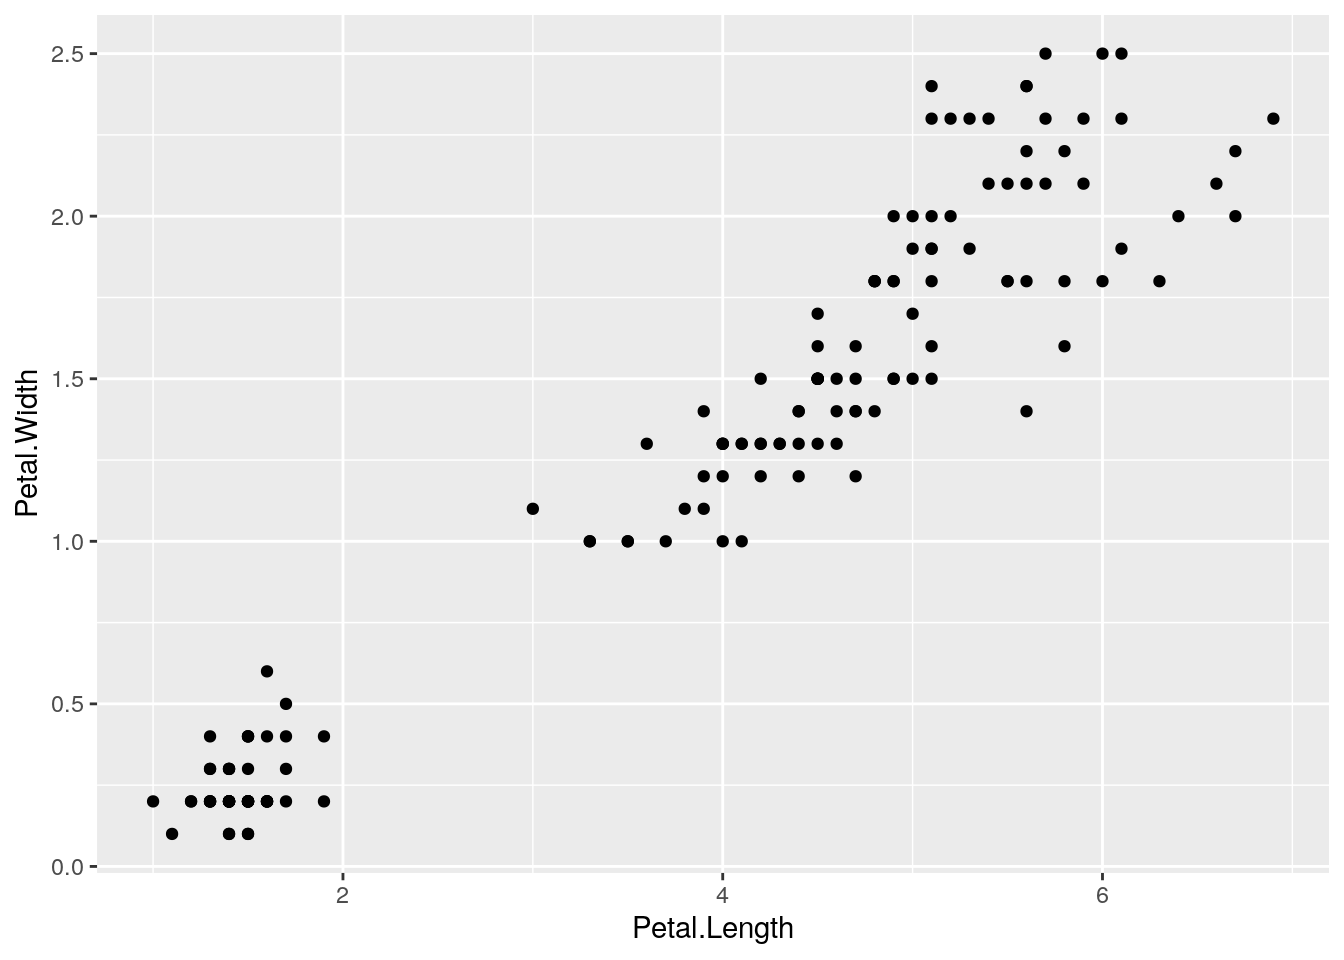
\includegraphics[width=1\linewidth]{03-gam_files/figure-latex/unnamed-chunk-12-1} 

}

\caption{vis.gam plot del modelo 2.}\label{fig:unnamed-chunk-12}
\end{figure}

Se pueden graficar los valores observados a campo y los predichos por el modelo. Cuanto mas alto sea el \(R_{adj}^{2}\), mas similares serán ambos valores.

\begin{Shaded}
\begin{Highlighting}[]
\CommentTok{\# generar datos para el gráfico }
\NormalTok{Base}\OtherTok{\textless{}{-}}\FunctionTok{as.data.table}\NormalTok{(base) }
\NormalTok{datas }\OtherTok{\textless{}{-}} \FunctionTok{rbindlist}\NormalTok{(}\FunctionTok{list}\NormalTok{(Base[, .(Pcy\_orgml, Fecha)], }
                        \FunctionTok{data.table}\NormalTok{(}\AttributeTok{Pcy\_orgml =}\NormalTok{ (modelo2}\SpecialCharTok{$}\NormalTok{gam)}\SpecialCharTok{$}\NormalTok{fitted.values,}
                                   \AttributeTok{Fecha =}\NormalTok{ Base[, Fecha])))}
\NormalTok{datas[, datos }\SpecialCharTok{:}\ErrorTok{=} \FunctionTok{c}\NormalTok{(}\FunctionTok{rep}\NormalTok{(}\StringTok{"Observados"}\NormalTok{, }\FunctionTok{nrow}\NormalTok{(Base)), }
                  \FunctionTok{rep}\NormalTok{(}\StringTok{"Predichos"}\NormalTok{, }\FunctionTok{nrow}\NormalTok{(Base)))]}

\CommentTok{\# generar el gráfico}
\FunctionTok{ggplot}\NormalTok{(}\AttributeTok{data =}\NormalTok{ datas, }\FunctionTok{aes}\NormalTok{(Fecha,Pcy\_orgml, }\AttributeTok{group =}\NormalTok{ datos))}\SpecialCharTok{+}
  \FunctionTok{geom\_line}\NormalTok{(}\FunctionTok{aes}\NormalTok{(}\AttributeTok{colour =}\NormalTok{ datos))}\SpecialCharTok{+}
  \FunctionTok{scale\_color\_manual}\NormalTok{(}\AttributeTok{values=}\FunctionTok{c}\NormalTok{(}\StringTok{"black"}\NormalTok{,}\StringTok{"red"}\NormalTok{))}\SpecialCharTok{+}
  \FunctionTok{labs}\NormalTok{(}\AttributeTok{x =} \StringTok{""}\NormalTok{, }\AttributeTok{y =} \StringTok{"Pcy (org/ml)"}\NormalTok{)}
\end{Highlighting}
\end{Shaded}

\includegraphics{03-gam_files/figure-latex/unnamed-chunk-13-1.pdf}

\hypertarget{agradecimientos}{%
\section{Agradecimientos}\label{agradecimientos}}

Un agradecimiento muy especial para los Profesores \textbf{Gerardo Cueto} y \textbf{Adriana Pérez} de la FCEN-UBA.

\hypertarget{multi1}{%
\chapter{Análisis multivariados I}\label{multi1}}

\textbf{Patricia E. García}\footnote{\href{mailto:garciapatriciaelizabeth@gmail.com}{\nolinkurl{garciapatriciaelizabeth@gmail.com}}}

Instituto de Investigaciones en Biodiversidad y Medioambiente (INIBIOMA, CONICET-UNComahue)

En esta unidad se verán ejemplos de ACP, NMDS, PERMANOVA

\hypertarget{anuxe1lisis-de-componentes-principales}{%
\section{Análisis de Componentes Principales}\label{anuxe1lisis-de-componentes-principales}}

\emph{Introducción}: Algunos sistemas no pueden definirse por sus características individuales, sino que deben verse en conjunto. Un ejemplo muy sencillo para entender este concepto es intentar describir una cara humana con un solo rasgo: la nariz.

\begin{figure}
\centering

\includegraphics{./images/nariz.png}
\caption{Se puede identificar una cara solo describiendo la nariz?}
\end{figure}

Para describir y reconocer una cara es necesario observar todas sus características: la nariz, los ojos, la boca, las cejas, etc. Es decir, múltiples dimensiones.

El \textbf{análisis de componentes principales (APC)} también conocido por siglas en inglés Principal Componentes Analysis PCA, es una poderosa herramienta estadística para describir un conjunto de datos.

Se basa en la reducción de la multidimensionalidad de una manera ``\emph{no supervisada}''.

Su principal objetivo es proyectar datos en las direcciones de \textbf{máxima varianza} y de este modo eliminar aquellas direcciones o planos que aporten menos información.

El ACP puede aplicarse antes de realizar un análisis de regresión o simplemente con fines exploratorios para ayudar a los investigadores a comprender relaciones entre las variables o descubrir patrones presentes en los datos.

\hypertarget{quuxe9-tipos-de-datos-usa-una-acp}{%
\subsection{¿Qué tipos de datos usa una ACP?}\label{quuxe9-tipos-de-datos-usa-una-acp}}

Utiliza principalmente variable \emph{numéricas continuas} que son las que efectivamente entran en el análisis. Estás variables se organizan en \textbf{columnas}, mientras que en las \textbf{filas} se organizan los individuos.

\begin{figure}
\centering
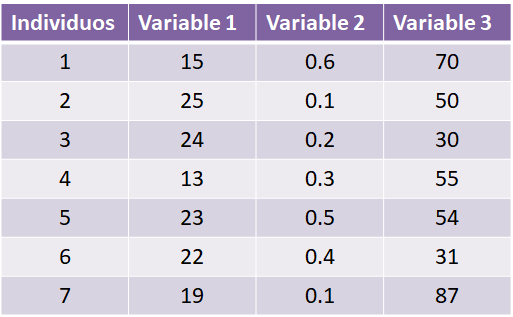
\includegraphics{./images/organi.png}
\caption{Organización de los datos}
\end{figure}

Estas bases de datos son de doble entrada, por lo que es posible analizarla desde el punto de vista de los individuos, de tal manera que \emph{individuos} que tiene características similares estarán más cerca.

Desde el punto de las \emph{variables}, se pueden analizar las relaciones entre las mismas. El análisis considera relaciones lineales entre las variables y usa coeficientes de correlación. Es importante utilizar la matriz de correlación para observar las relaciones más importantes entre las variables.

\hypertarget{cuxf3mo-funciona-el-anuxe1lisis}{%
\subsection{¿Cómo funciona el análisis?}\label{cuxf3mo-funciona-el-anuxe1lisis}}

El funcionamiento del análisis es muy sencillo, trata de buscar la \emph{dirección o componente} que maximice la variación de datos. Es decir que el primer plano/componente trata de capturar la mayor dispersión de los datos.

\begin{figure}
\centering
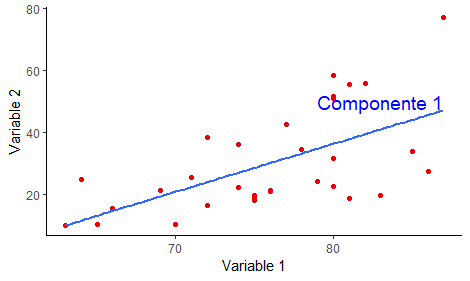
\includegraphics{./images/compo_1.png}
\caption{El primer componente}
\end{figure}

En el ACP, luego que se encontró el primer componente que maximizó la dispersión de los datos, el segundo componente es ortogonal, es decir a 90°.

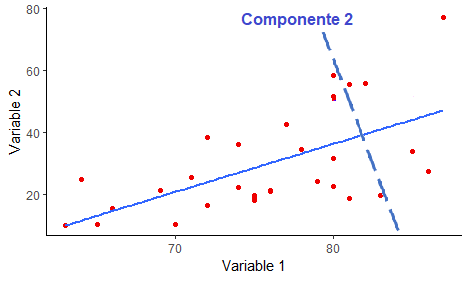
\includegraphics{./images/compo_2.png}

\hypertarget{ahora-manos-a-la-obra-miremos-datos}{%
\subsection{Ahora manos a la obra: miremos datos}\label{ahora-manos-a-la-obra-miremos-datos}}

En RStudio importamos la base de datos ambientales de \href{https://doi.org/10.1016/j.chemosphere.2018.02.103}{Castro Berman et al., 2018}, disponible como \textbf{data\_cursoR.xlsx} en \href{https://github.com/Limno-con-R/CILCAL2023/tree/main/datasets}{GitHub Limno-con-R/CILCAL2023}. Recuerden guardar el archivo en una carpeta llamada \emph{data}, dentro del \textbf{Directorio de Trabajo} del \textbf{Proyecto} que creamos para esta Unidad (ver cómo hacerlo en la Unidad \ref{intro}).

\begin{Shaded}
\begin{Highlighting}[]
\FunctionTok{library}\NormalTok{(readxl)}
\NormalTok{datos }\OtherTok{\textless{}{-}}  \FunctionTok{read\_excel}\NormalTok{(}\StringTok{"data/data\_cursoR.xlsx"}\NormalTok{, }
    \AttributeTok{col\_types =} \FunctionTok{c}\NormalTok{(}\StringTok{"text"}\NormalTok{, }\StringTok{"numeric"}\NormalTok{, }\StringTok{"numeric"}\NormalTok{, }
        \StringTok{"numeric"}\NormalTok{, }\StringTok{"numeric"}\NormalTok{, }\StringTok{"numeric"}\NormalTok{, }
        \StringTok{"numeric"}\NormalTok{, }\StringTok{"numeric"}\NormalTok{, }\StringTok{"numeric"}\NormalTok{, }
        \StringTok{"numeric"}\NormalTok{, }\StringTok{"numeric"}\NormalTok{, }\StringTok{"numeric"}\NormalTok{, }
        \StringTok{"numeric"}\NormalTok{, }\StringTok{"numeric"}\NormalTok{, }\StringTok{"numeric"}\NormalTok{, }
        \StringTok{"numeric"}\NormalTok{, }\StringTok{"numeric"}\NormalTok{, }\StringTok{"numeric"}\NormalTok{), }
    \AttributeTok{na =} \StringTok{"NA"}\NormalTok{)}
\end{Highlighting}
\end{Shaded}

\begin{verbatim}
## New names:
## * `` -> `...1`
\end{verbatim}

\begin{Shaded}
\begin{Highlighting}[]
\NormalTok{datos }\OtherTok{\textless{}{-}} \FunctionTok{data.frame}\NormalTok{(datos, }\AttributeTok{row.names =} \DecValTok{1}\NormalTok{)}
\FunctionTok{head}\NormalTok{(datos)}
\end{Highlighting}
\end{Shaded}

\begin{verbatim}
##       ELEVACION  LATITUD LONGITUD Temp Secchi   DO   pH Conductivity   NTU  TON
## SL_13        62 -38.4184 -61.7594   17     44 11.8 8.55         0.32  15.7 3438
## SL_17        20 -38.9263 -61.3687    7      8  8.0 8.53         3.43 363.0 4010
## SL_18       119 -38.3474 -60.4527   14     12  9.0 8.84         4.05 110.0 4200
## SL_19        89 -38.4273 -60.3181   14     24 10.8 8.54         1.10  54.4 4738
## SL_20        64 -38.5216 -60.1404   10      9  9.0 8.44         3.25 206.0 7470
## SL_21       194 -38.0508 -60.0340   11     16 10.0 8.30         3.35 129.0 4256
##       TDON   SPM   POM   TP    TDP  Chl.a    DOC
## SL_13 2565  11.7   9.2  124    0.1   3.79   4.55
## SL_17 2890 377.5 103.4  272  114.0  68.63  10.98
## SL_18 3909  71.0  23.4 1009  833.0  54.36 253.50
## SL_19 4424  30.9  23.4  162    4.0  66.75  10.12
## SL_20 5107 186.6  62.5  727  456.0 475.36  95.43
## SL_21 3237 111.0  33.4 1365 1363.0  61.81 177.70
\end{verbatim}

La base de datos que importamos contiene información acerca de la localización geográfica de los sitios y las variables físico-químicas.

\begin{Shaded}
\begin{Highlighting}[]
\FunctionTok{summary}\NormalTok{(datos)}
\end{Highlighting}
\end{Shaded}

\begin{verbatim}
##    ELEVACION         LATITUD          LONGITUD           Temp      
##  Min.   :-16.00   Min.   :-38.93   Min.   :-63.09   Min.   : 7.00  
##  1st Qu.: 10.00   1st Qu.:-37.49   1st Qu.:-62.25   1st Qu.:15.00  
##  Median : 58.50   Median :-36.84   Median :-60.23   Median :17.50  
##  Mean   : 73.65   Mean   :-36.62   Mean   :-60.13   Mean   :18.52  
##  3rd Qu.:104.00   3rd Qu.:-35.69   3rd Qu.:-57.98   3rd Qu.:22.25  
##  Max.   :246.00   Max.   :-34.48   Max.   :-56.98   Max.   :30.00  
##                                                                    
##      Secchi             DO               pH         Conductivity    
##  Min.   :  7.00   Min.   : 5.000   Min.   :8.000   Min.   :  0.320  
##  1st Qu.: 12.00   1st Qu.: 8.725   1st Qu.:8.557   1st Qu.:  1.215  
##  Median : 18.00   Median :10.300   Median :8.795   Median :  2.615  
##  Mean   : 29.44   Mean   :10.238   Mean   :8.762   Mean   :  7.968  
##  3rd Qu.: 37.75   3rd Qu.:11.050   3rd Qu.:8.982   3rd Qu.:  5.513  
##  Max.   :140.00   Max.   :20.000   Max.   :9.400   Max.   :202.100  
##                                                                     
##       NTU              TON             TDON           SPM        
##  Min.   :  2.70   Min.   : 2856   Min.   :1926   Min.   :  6.70  
##  1st Qu.: 27.90   1st Qu.: 4104   1st Qu.:3052   1st Qu.: 36.20  
##  Median : 83.25   Median : 4872   Median :3478   Median : 75.45  
##  Mean   : 88.67   Mean   : 5063   Mean   :3790   Mean   :116.83  
##  3rd Qu.:110.00   3rd Qu.: 5323   3rd Qu.:4356   3rd Qu.:128.53  
##  Max.   :363.00   Max.   :10830   Max.   :7235   Max.   :788.40  
##                                                                  
##       POM               TP              TDP             Chl.a       
##  Min.   :  6.70   Min.   :  46.0   Min.   :   0.1   Min.   :  1.58  
##  1st Qu.: 20.00   1st Qu.: 324.0   1st Qu.: 114.0   1st Qu.: 15.80  
##  Median : 29.60   Median : 533.0   Median : 302.0   Median : 52.05  
##  Mean   : 40.80   Mean   : 766.1   Mean   : 560.3   Mean   : 87.80  
##  3rd Qu.: 47.92   3rd Qu.: 820.5   3rd Qu.: 624.0   3rd Qu.: 89.13  
##  Max.   :344.00   Max.   :4538.0   Max.   :4140.0   Max.   :981.06  
##                                                                     
##       DOC         
##  Min.   :   1.26  
##  1st Qu.:  12.36  
##  Median :  19.45  
##  Mean   :  93.22  
##  3rd Qu.:  97.58  
##  Max.   :1010.00  
##  NA's   :1
\end{verbatim}

\begin{verbatim}
##    ELEVACION         LATITUD          LONGITUD           Temp      
##  Min.   :-16.00   Min.   :-38.93   Min.   :-63.09   Min.   : 7.00  
##  1st Qu.: 10.00   1st Qu.:-37.49   1st Qu.:-62.25   1st Qu.:15.00  
##  Median : 58.50   Median :-36.84   Median :-60.23   Median :17.50  
##  Mean   : 73.65   Mean   :-36.62   Mean   :-60.13   Mean   :18.52  
##  3rd Qu.:104.00   3rd Qu.:-35.69   3rd Qu.:-57.98   3rd Qu.:22.25  
##  Max.   :246.00   Max.   :-34.48   Max.   :-56.98   Max.   :30.00  
##                                                                    
##      Secchi             DO               pH         Conductivity    
##  Min.   :  7.00   Min.   : 5.000   Min.   :8.000   Min.   :  0.320  
##  1st Qu.: 12.00   1st Qu.: 8.725   1st Qu.:8.557   1st Qu.:  1.215  
##  Median : 18.00   Median :10.300   Median :8.795   Median :  2.615  
##  Mean   : 29.44   Mean   :10.238   Mean   :8.762   Mean   :  7.968  
##  3rd Qu.: 37.75   3rd Qu.:11.050   3rd Qu.:8.982   3rd Qu.:  5.513  
##  Max.   :140.00   Max.   :20.000   Max.   :9.400   Max.   :202.100  
##                                                                     
##       NTU              TON             TDON           SPM        
##  Min.   :  2.70   Min.   : 2856   Min.   :1926   Min.   :  6.70  
##  1st Qu.: 27.90   1st Qu.: 4104   1st Qu.:3052   1st Qu.: 36.20  
##  Median : 83.25   Median : 4872   Median :3478   Median : 75.45  
##  Mean   : 88.67   Mean   : 5063   Mean   :3790   Mean   :116.83  
##  3rd Qu.:110.00   3rd Qu.: 5323   3rd Qu.:4356   3rd Qu.:128.53  
##  Max.   :363.00   Max.   :10830   Max.   :7235   Max.   :788.40  
##                                                                  
##       POM               TP              TDP             Chl.a       
##  Min.   :  6.70   Min.   :  46.0   Min.   :   0.1   Min.   :  1.58  
##  1st Qu.: 20.00   1st Qu.: 324.0   1st Qu.: 114.0   1st Qu.: 15.80  
##  Median : 29.60   Median : 533.0   Median : 302.0   Median : 52.05  
##  Mean   : 40.80   Mean   : 766.1   Mean   : 560.3   Mean   : 87.80  
##  3rd Qu.: 47.92   3rd Qu.: 820.5   3rd Qu.: 624.0   3rd Qu.: 89.13  
##  Max.   :344.00   Max.   :4538.0   Max.   :4140.0   Max.   :981.06  
##                                                                     
##       DOC         
##  Min.   :   1.26  
##  1st Qu.:  12.36  
##  Median :  19.45  
##  Mean   :  93.22  
##  3rd Qu.:  97.58  
##  Max.   :1010.00  
##  NA's   :1
\end{verbatim}

En resumen, tenemos 52 observaciones (individuos) y 17 variables. De las variables presentes las primeras 3 (Elevación, Longitud y Latitud) corresponden a la localización de los ambientes.

Las variables son continuas y cada una está medida de manera distintas por lo que cada una tiene su unidad y a su vez su variación. Debido a esto es necesario \textbf{estandarizar} y \textbf{centrar} las variables. La estandarización simplemente le resta a cada observación el promedio de la variable y la divide por la desviación estandar de la variable. Mientras que centrar significa que se mueve la nube de puntos de los individuos al centro de gravedad.

\begin{Shaded}
\begin{Highlighting}[]
\NormalTok{?scale }\CommentTok{\# el comando para estandarizar los datos}
\end{Highlighting}
\end{Shaded}

\begin{verbatim}
## starting httpd help server ... done
\end{verbatim}

\begin{Shaded}
\begin{Highlighting}[]
\NormalTok{datos.stand }\OtherTok{\textless{}{-}} \FunctionTok{data.frame}\NormalTok{(}\FunctionTok{scale}\NormalTok{(datos [}\DecValTok{4}\SpecialCharTok{:}\DecValTok{17}\NormalTok{], }\AttributeTok{center =}\NormalTok{ T))}
\end{Highlighting}
\end{Shaded}

Para este ejemplo solo usé las variables físico-químicas, para ello utilicé los corchetes e indiqué el número de columnas que quería se estandarizaran, de la columna 4 a la columna 17: \textbf{{[}4:17{]}}.

El comando para realizar el análisis de componentes principales , está en el paquete FactoMiner. Este paquete es muy versatil y se mantiene actualizado. Aqui adjunto el link:

\href{http://factominer.free.fr}{FactoMineR}

\begin{verbatim}
## Warning: package 'FactoMineR' was built under R version 4.2.3
\end{verbatim}

\begin{verbatim}
## Warning in PCA(datos.stand[-2], graph = FALSE): Missing values are imputed by
## the mean of the variable: you should use the imputePCA function of the missMDA
## package
\end{verbatim}

¡Recibimos un \textbf{\emph{mensaje de advertencia}}! Este mensaje nos indica que hay valores faltantes y que el comando va a usar el promedio de la variable en las celdas donde falten datos.

\textbf{Importante}: algunos análisis son muy sensibles a la falta de datos.

¡Listo hemos realizado el analisis de ACP! El objeto ``res.pca'' es una lista que tiene toda la información.

\begin{Shaded}
\begin{Highlighting}[]
\FunctionTok{print}\NormalTok{(res.pca)}
\end{Highlighting}
\end{Shaded}

\begin{verbatim}
## **Results for the Principal Component Analysis (PCA)**
## The analysis was performed on 52 individuals, described by 13 variables
## *The results are available in the following objects:
## 
##    name               description                          
## 1  "$eig"             "eigenvalues"                        
## 2  "$var"             "results for the variables"          
## 3  "$var$coord"       "coord. for the variables"           
## 4  "$var$cor"         "correlations variables - dimensions"
## 5  "$var$cos2"        "cos2 for the variables"             
## 6  "$var$contrib"     "contributions of the variables"     
## 7  "$ind"             "results for the individuals"        
## 8  "$ind$coord"       "coord. for the individuals"         
## 9  "$ind$cos2"        "cos2 for the individuals"           
## 10 "$ind$contrib"     "contributions of the individuals"   
## 11 "$call"            "summary statistics"                 
## 12 "$call$centre"     "mean of the variables"              
## 13 "$call$ecart.type" "standard error of the variables"    
## 14 "$call$row.w"      "weights for the individuals"        
## 15 "$call$col.w"      "weights for the variables"
\end{verbatim}

\hypertarget{anuxe1lisis-de-los-resultados}{%
\subsubsection{Análisis de los resultados}\label{anuxe1lisis-de-los-resultados}}

El ACP calcula los autovalores (eigenvalues) y autovectores propios a partir de la matriz de covarianzas. El cálculo de los vectores depende de la cantidad de dimensiones de los datos. Los autovalores no son más que la magnitud de los autovectores, ambos ayudan a calcular los Componentes principales.

\begin{Shaded}
\begin{Highlighting}[]
\NormalTok{eigenvalues }\OtherTok{\textless{}{-}}\NormalTok{ res.pca}\SpecialCharTok{$}\NormalTok{eig}\CommentTok{\# eigenvalues}
\FunctionTok{head}\NormalTok{(eigenvalues[, }\DecValTok{1}\SpecialCharTok{:}\DecValTok{3}\NormalTok{])}
\end{Highlighting}
\end{Shaded}

\begin{verbatim}
##        eigenvalue percentage of variance cumulative percentage of variance
## comp 1  4.1797364              32.151818                          32.15182
## comp 2  3.5439409              27.261084                          59.41290
## comp 3  1.3449952              10.346117                          69.75902
## comp 4  1.0490855               8.069888                          77.82891
## comp 5  0.9618192               7.398609                          85.22752
## comp 6  0.8132415               6.255704                          91.48322
\end{verbatim}

En la primer columna se observa el valor del eigenvalue, en la segunda columna se observa el porcentaje de variación explicada. En la tercera columna se muestra el porcentaje de variación acumulada.

Un paquete útil para mejorar los gráficos de los analisis multivariados es \textbf{factoextra}.

\begin{verbatim}
## Warning: package 'factoextra' was built under R version 4.2.3
\end{verbatim}

\begin{verbatim}
## Loading required package: ggplot2
\end{verbatim}

\begin{verbatim}
## Warning: package 'ggplot2' was built under R version 4.2.2
\end{verbatim}

\begin{verbatim}
## Welcome! Want to learn more? See two factoextra-related books at https://goo.gl/ve3WBa
\end{verbatim}

\includegraphics{04-multi1_b_files/figure-latex/unnamed-chunk-8-1.pdf}

Los \textbf{eigenvalues} se utilizan para determinar el número de componentes que deben conservarse. Existen dos maneras frecuentes de analizar estos eigenvalues, por un lado muchos investigadores utilizan los eigenvalues \textgreater{} 1. Otra manera de determinar el número de componentes es por la cantidad de variación explicada, muchos usan \textgreater{} 70\% de la variabilidad de los datos.

En este ejemplo, los primeros dos planos solo explican un 59.5\% de la variabilidad de los datos y al usar un 3 eje se explica 69.8\%. Decido usar 3 ejes para describir estos datos.

\hypertarget{visualizar-los-datos}{%
\subsubsection{Visualizar los datos}\label{visualizar-los-datos}}

Ahora vamos a visualizar los tres ejes. Como habíamos dicho previamente, el ACP genera gráficos de los individuos y de las variables. Actualmente es más frecuente usar gráficos en los que se observen ambos: los individuos y las variables. Este tipo de gráficos se denomina biplots.

\begin{Shaded}
\begin{Highlighting}[]
\NormalTok{?fviz\_pca\_biplot}
\FunctionTok{fviz\_pca\_biplot}\NormalTok{(res.pca,  }\AttributeTok{repel=}\ConstantTok{TRUE}\NormalTok{, }\AttributeTok{invisible =} \StringTok{"quali"}\NormalTok{)}\SpecialCharTok{+}\FunctionTok{theme\_classic}\NormalTok{()}
\end{Highlighting}
\end{Shaded}

\begin{verbatim}
## Warning: ggrepel: 39 unlabeled data points (too many overlaps). Consider
## increasing max.overlaps
\end{verbatim}

\includegraphics{04-multi1_b_files/figure-latex/unnamed-chunk-9-1.pdf}

El gráfico muestra los ejes o componentes 1 y 2. A simple vista se observa que algunos individuos, como SL\_34 por ejemplo es la muestra que tiene mas DOC (carbono orgánico disuelto), mientras que la muestra SL\_50 es la que presentó la mayor cantidad de POM (materia orgánica particulada).

\emph{Interpretación}: el primer componente (Dim1 32.\%) divide a las muestras que tienen más DOC, más conductividad, más TP hacía la derecha del gráfico. El componente 2, parece que divide a las muestras de acuerdo a la POM, la clorofila a, la salinidad.

Ahora vamos a ver el componente 1 vs el componente 3.

\begin{Shaded}
\begin{Highlighting}[]
\FunctionTok{fviz\_pca\_biplot}\NormalTok{(res.pca, }\AttributeTok{axes=}\FunctionTok{c}\NormalTok{(}\DecValTok{1}\NormalTok{,}\DecValTok{3}\NormalTok{),  }\AttributeTok{repel=}\ConstantTok{TRUE}\NormalTok{, }\AttributeTok{invisible =} \StringTok{"quali"}\NormalTok{)}\SpecialCharTok{+}\FunctionTok{theme\_classic}\NormalTok{()}
\end{Highlighting}
\end{Shaded}

\begin{verbatim}
## Warning: ggrepel: 24 unlabeled data points (too many overlaps). Consider
## increasing max.overlaps
\end{verbatim}

\includegraphics{04-multi1_b_files/figure-latex/unnamed-chunk-10-1.pdf}

Una función importante del paquete FactoMiner, es el comando dimdesc. El mismo se utiliza para identificar las variables más significativamente asociadas a un componente.

\begin{Shaded}
\begin{Highlighting}[]
\FunctionTok{dimdesc}\NormalTok{(res.pca, }\AttributeTok{axes =} \FunctionTok{c}\NormalTok{(}\DecValTok{1}\SpecialCharTok{:}\DecValTok{3}\NormalTok{), }\AttributeTok{proba =} \FloatTok{0.05}\NormalTok{)}
\end{Highlighting}
\end{Shaded}

\begin{verbatim}
## $Dim.1
## 
## Link between the variable and the continuous variables (R-square)
## =================================================================================
##              correlation      p.value
## SPM            0.8005755 1.052112e-12
## TP             0.7292919 8.700526e-10
## DOC            0.7269277 1.048135e-09
## Conductivity   0.6820821 2.578475e-08
## TDP            0.6440372 2.589279e-07
## POM            0.5824318 5.906561e-06
## TDON           0.5749478 8.275646e-06
## TON            0.5672584 1.160335e-05
## Chl.a          0.4838790 2.787599e-04
## pH             0.4499121 8.187113e-04
## DO             0.3463183 1.190357e-02
## 
## $Dim.2
## 
## Link between the variable and the continuous variables (R-square)
## =================================================================================
##              correlation      p.value
## POM            0.7266597 1.070368e-09
## Chl.a          0.7136585 2.879319e-09
## NTU            0.5945254 3.363780e-06
## TON            0.5361705 4.189718e-05
## DO             0.4590453 6.194896e-04
## TDON           0.4178871 2.052244e-03
## Conductivity  -0.4936215 2.003631e-04
## TP            -0.5713221 9.715629e-06
## DOC           -0.6187953 1.011371e-06
## TDP           -0.6865882 1.917673e-08
## 
## $Dim.3
## 
## Link between the variable and the continuous variables (R-square)
## =================================================================================
##      correlation      p.value
## pH     0.4460824 9.181604e-04
## TON    0.4261880 1.631046e-03
## TDON   0.3729687 6.466085e-03
## SPM   -0.5178939 8.417748e-05
## NTU   -0.6197587 9.622302e-07
\end{verbatim}

Estos resultados nos permiten asociar variables a los distintos ejes/componentes. Se puede inclusive establecer un criterio ya que usa coeficientes de correlación. Para este ejemplo, se puede usar las variables que tienen una correlación \textgreater0.6 con el eje. Para el componente principal 1, que explica (32.2\%), las variables asociadas a este componente son DOC, TP, TDP, conductivity y SPM. Para el componente principal 2 (27.3\%), está asociado a POM, clorofila a y NTU (salinidad). Finalmente, el componente principal 3 (10.3\%) estaría asociado de manera negativa solo a la salinidad (NTU). El signo de la correlación indica la dirección de la correlación.

\hypertarget{crear-una-condiciuxf3n-para-colorear-los-individuos}{%
\subsection{Crear una condición para colorear los individuos}\label{crear-una-condiciuxf3n-para-colorear-los-individuos}}

A veces es útil crear alguna condición (variable categórica) para colorear los individuos y quizás empezar a ver patrones más claros. En este voy a usar la variable ``secchi'' para colorear a los individuos. Si la variable secchi es menor o igual a 20 entonces voy a llamar a la laguna como ``turbia'' mientras que si es mayor a 20, la voy a denominar laguna ``clara''.

\begin{Shaded}
\begin{Highlighting}[]
\NormalTok{datos}\SpecialCharTok{$}\NormalTok{condicion }\OtherTok{\textless{}{-}} \FunctionTok{as.factor}\NormalTok{(}\FunctionTok{ifelse}\NormalTok{(datos}\SpecialCharTok{$}\NormalTok{Secchi}\SpecialCharTok{\textless{}=}\DecValTok{20}\NormalTok{, }\StringTok{"Turbia"}\NormalTok{, }\StringTok{"Clara"}\NormalTok{))}
\end{Highlighting}
\end{Shaded}

Cree una nueva variable llamada condicion

\begin{Shaded}
\begin{Highlighting}[]
\FunctionTok{fviz\_pca\_biplot}\NormalTok{(res.pca,  }\AttributeTok{repel=}\ConstantTok{TRUE}\NormalTok{, }\AttributeTok{invisible =} \StringTok{"quali"}\NormalTok{, }\AttributeTok{habillage =}\NormalTok{ datos}\SpecialCharTok{$}\NormalTok{condicion, }\AttributeTok{geom =}\NormalTok{ (}\StringTok{"point"}\NormalTok{))}\SpecialCharTok{+}\FunctionTok{theme\_classic}\NormalTok{()}
\end{Highlighting}
\end{Shaded}

\includegraphics{04-multi1_b_files/figure-latex/unnamed-chunk-13-1.pdf}

\hypertarget{refinando-el-modelo}{%
\subsection{Refinando el modelo}\label{refinando-el-modelo}}

El APC explica aproximadamente un 69\% usando tres ejes. En el próximo paso vamos a seleccionar solo las variables disueltas: DOC, pH, TDON, DO, TDP, chla. y conductivity.

\begin{Shaded}
\begin{Highlighting}[]
\NormalTok{data.stan.sel }\OtherTok{\textless{}{-}}\NormalTok{datos.stand [,}\FunctionTok{c}\NormalTok{(}\DecValTok{3}\SpecialCharTok{:}\DecValTok{5}\NormalTok{,}\DecValTok{8}\NormalTok{,}\DecValTok{12}\SpecialCharTok{:}\DecValTok{14}\NormalTok{)]}
\end{Highlighting}
\end{Shaded}

Vuelvo a realizar el analisis de ACP:

\begin{Shaded}
\begin{Highlighting}[]
\NormalTok{res.pca2 }\OtherTok{\textless{}{-}}\FunctionTok{PCA}\NormalTok{(data.stan.sel, }\AttributeTok{graph=}\ConstantTok{FALSE}\NormalTok{)}
\end{Highlighting}
\end{Shaded}

\begin{verbatim}
## Warning in PCA(data.stan.sel, graph = FALSE): Missing values are imputed by
## the mean of the variable: you should use the imputePCA function of the missMDA
## package
\end{verbatim}

\begin{Shaded}
\begin{Highlighting}[]
\NormalTok{eigenvalues2 }\OtherTok{\textless{}{-}}\NormalTok{ res.pca2}\SpecialCharTok{$}\NormalTok{eig}\CommentTok{\# eigenvalues}
\FunctionTok{head}\NormalTok{(eigenvalues2[, }\DecValTok{1}\SpecialCharTok{:}\DecValTok{3}\NormalTok{])}
\end{Highlighting}
\end{Shaded}

\begin{verbatim}
##        eigenvalue percentage of variance cumulative percentage of variance
## comp 1  2.7477587              39.253696                          39.25370
## comp 2  1.8792045              26.845778                          66.09947
## comp 3  0.8578634              12.255191                          78.35467
## comp 4  0.7497849              10.711212                          89.06588
## comp 5  0.4279332               6.113331                          95.17921
## comp 6  0.2531477               3.616395                          98.79560
\end{verbatim}

Biplot:

\begin{Shaded}
\begin{Highlighting}[]
\FunctionTok{fviz\_pca\_biplot}\NormalTok{(res.pca2,  }\AttributeTok{repel=}\ConstantTok{TRUE}\NormalTok{, }\AttributeTok{invisible =} \StringTok{"quali"}\NormalTok{, }\AttributeTok{habillage =}\NormalTok{ datos}\SpecialCharTok{$}\NormalTok{condicion, }\AttributeTok{geom =}\NormalTok{ (}\StringTok{"point"}\NormalTok{))}\SpecialCharTok{+}\FunctionTok{theme\_classic}\NormalTok{()}
\end{Highlighting}
\end{Shaded}

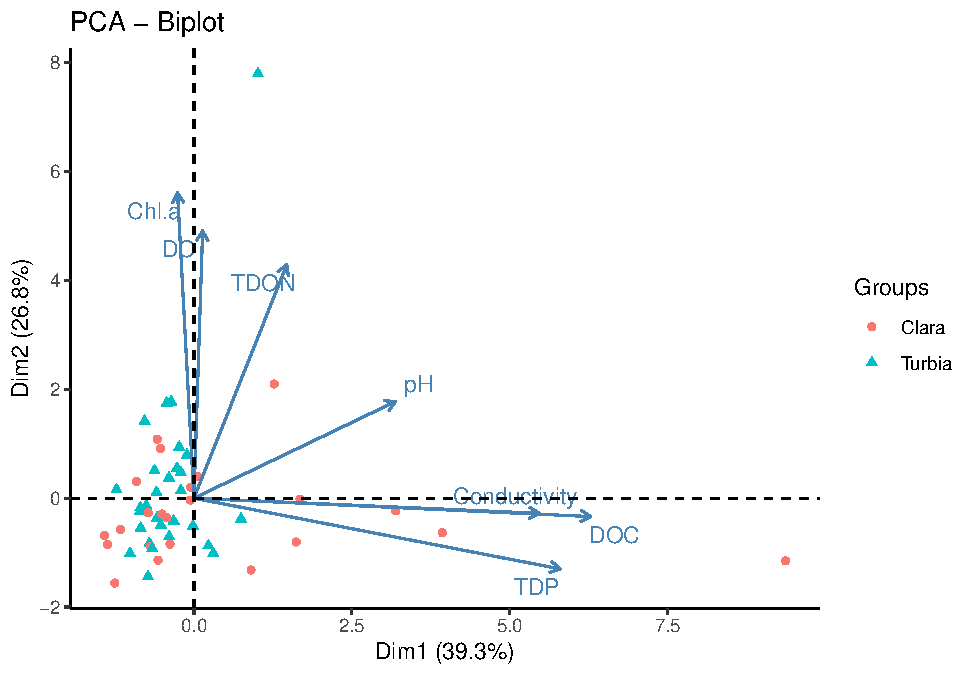
\includegraphics{04-multi1_b_files/figure-latex/unnamed-chunk-17-1.pdf}

\begin{Shaded}
\begin{Highlighting}[]
\FunctionTok{fviz\_pca\_biplot}\NormalTok{(res.pca2,  }\AttributeTok{axes=} \FunctionTok{c}\NormalTok{(}\DecValTok{1}\NormalTok{,}\DecValTok{3}\NormalTok{), }\AttributeTok{repel=}\ConstantTok{TRUE}\NormalTok{, }\AttributeTok{invisible =} \StringTok{"quali"}\NormalTok{, }\AttributeTok{habillage =}\NormalTok{ datos}\SpecialCharTok{$}\NormalTok{condicion, }\AttributeTok{geom =}\NormalTok{ (}\StringTok{"point"}\NormalTok{))}\SpecialCharTok{+}\FunctionTok{theme\_classic}\NormalTok{()}
\end{Highlighting}
\end{Shaded}

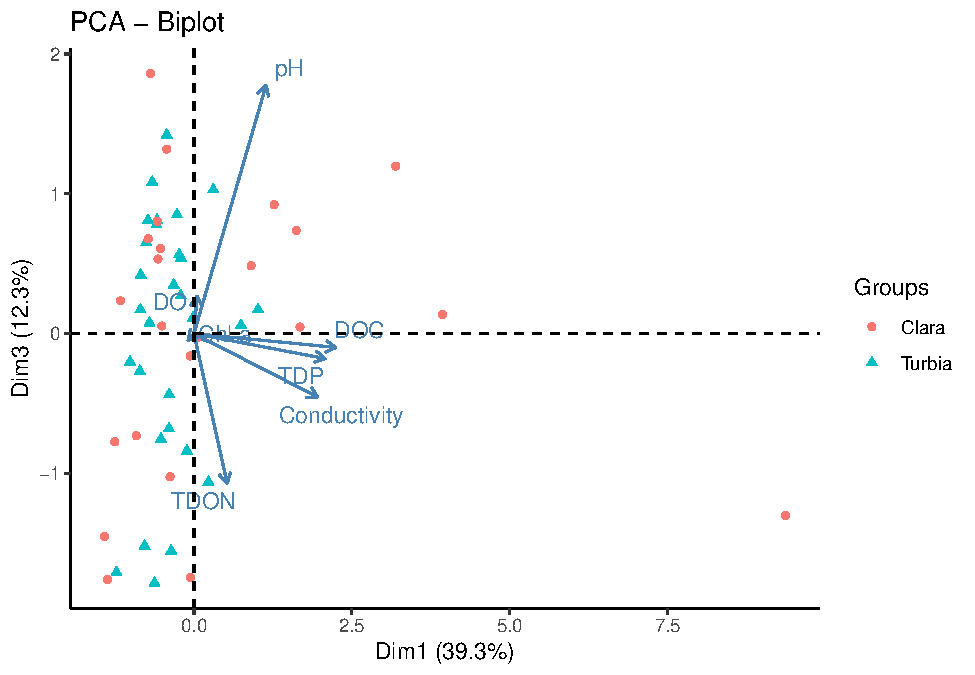
\includegraphics{04-multi1_b_files/figure-latex/unnamed-chunk-18-1.pdf}

El nuevo ACP con las variables seleccionadas, explica un 78\% de la variabilidad total de los datos, teniendo en cuenta los primeros 3 ejes. Considero que este modelo refinado es mucho mejor que el anterior.

\hypertarget{nmds}{%
\section{NMDS}\label{nmds}}

El escalamiento multidimensional no métrico, mejor conocido por sus siglas en ingles (\textbf{Non-metric Multidimensional Scaling}), es un método de análisis estadístico multivariado que representa mediciones de \emph{similaridad} (o disimilaridad) entre pares de objetos como distancias entre puntos de un espacio de dimensión reducida. El objetivo fundamental del \textbf{NMDS} es generar una representación gráfica de los objetos en un espacio de modo que sus posiciones relativas sean el reflejo de su proximidad. A diferencia de otros métodos de escalamientos, el NMDS utiliza ordenes de rango, por lo que es una técnica extremadamente flexible que puede adaptarse a una gran variedad de datos.

\begin{verbatim}
## Warning: package 'vegan' was built under R version 4.2.3
\end{verbatim}

\begin{verbatim}
## Loading required package: permute
\end{verbatim}

\begin{verbatim}
## Loading required package: lattice
\end{verbatim}

\begin{verbatim}
## This is vegan 2.6-4
\end{verbatim}

Vamos a usar las variables seleccionadas en el segundo ACP, es decir las variables más relacionadas con la fracción disuelta.

\begin{Shaded}
\begin{Highlighting}[]
\NormalTok{disueltos }\OtherTok{\textless{}{-}}\NormalTok{ datos[,}\FunctionTok{c}\NormalTok{(}\DecValTok{6}\SpecialCharTok{:}\DecValTok{8}\NormalTok{,}\DecValTok{11}\NormalTok{,}\DecValTok{15}\SpecialCharTok{:}\DecValTok{17}\NormalTok{)]}
\FunctionTok{summary}\NormalTok{(disueltos)}
\end{Highlighting}
\end{Shaded}

\begin{verbatim}
##        DO               pH         Conductivity          TDON     
##  Min.   : 5.000   Min.   :8.000   Min.   :  0.320   Min.   :1926  
##  1st Qu.: 8.725   1st Qu.:8.557   1st Qu.:  1.215   1st Qu.:3052  
##  Median :10.300   Median :8.795   Median :  2.615   Median :3478  
##  Mean   :10.238   Mean   :8.762   Mean   :  7.968   Mean   :3790  
##  3rd Qu.:11.050   3rd Qu.:8.982   3rd Qu.:  5.513   3rd Qu.:4356  
##  Max.   :20.000   Max.   :9.400   Max.   :202.100   Max.   :7235  
##                                                                   
##       TDP             Chl.a             DOC         
##  Min.   :   0.1   Min.   :  1.58   Min.   :   1.26  
##  1st Qu.: 114.0   1st Qu.: 15.80   1st Qu.:  12.36  
##  Median : 302.0   Median : 52.05   Median :  19.45  
##  Mean   : 560.3   Mean   : 87.80   Mean   :  93.22  
##  3rd Qu.: 624.0   3rd Qu.: 89.13   3rd Qu.:  97.58  
##  Max.   :4140.0   Max.   :981.06   Max.   :1010.00  
##                                    NA's   :1
\end{verbatim}

Algunos análisis exploratorios multivariados son sensibles a los datos faltantes. Como se puede observar, la variable DOC tiene un dato faltante. En este caso, lo mejor es sacar esa fila del análisis.

\begin{Shaded}
\begin{Highlighting}[]
\NormalTok{disueltos }\OtherTok{\textless{}{-}}\NormalTok{ disueltos[}\SpecialCharTok{{-}}\DecValTok{17}\NormalTok{,]}
\NormalTok{condicion }\OtherTok{\textless{}{-}} \FunctionTok{data.frame}\NormalTok{(datos}\SpecialCharTok{$}\NormalTok{condicion)}
\NormalTok{condicion }\OtherTok{\textless{}{-}}\NormalTok{ condicion [}\SpecialCharTok{{-}}\FunctionTok{c}\NormalTok{(}\DecValTok{17}\NormalTok{),]}\DocumentationTok{\#\# hay que sacar la misma fila de la variable condicion}
\end{Highlighting}
\end{Shaded}

Ahora se estandarizan los datos y luego se los convierte a distancias euclidianas para luego realizar el análisis.

\begin{Shaded}
\begin{Highlighting}[]
\FunctionTok{set.seed}\NormalTok{(}\DecValTok{2306}\NormalTok{)}\CommentTok{\# generar resultados reproducibles}
\NormalTok{dis.stan }\OtherTok{\textless{}{-}}\FunctionTok{decostand}\NormalTok{(disueltos, }\StringTok{"stand"}\NormalTok{) }\CommentTok{\# estandarizar: variables ambientales en diferentes unidades}
\NormalTok{dis.dist }\OtherTok{\textless{}{-}}\FunctionTok{vegdist}\NormalTok{(dis.stan, }\StringTok{"euc"}\NormalTok{) }\CommentTok{\# distancia euclidiana}
\NormalTok{res.nmds }\OtherTok{\textless{}{-}}\FunctionTok{metaMDS}\NormalTok{(dis.dist,  }\AttributeTok{trymax =} \DecValTok{500}\NormalTok{) }\CommentTok{\# NMDS}
\end{Highlighting}
\end{Shaded}

\begin{verbatim}
## Run 0 stress 0.08172658 
## Run 1 stress 0.08190544 
## ... Procrustes: rmse 0.01185868  max resid 0.06039221 
## Run 2 stress 0.08129024 
## ... New best solution
## ... Procrustes: rmse 0.01390953  max resid 0.05964353 
## Run 3 stress 0.08801438 
## Run 4 stress 0.08189141 
## Run 5 stress 0.0846288 
## Run 6 stress 0.08169404 
## ... Procrustes: rmse 0.02381188  max resid 0.116934 
## Run 7 stress 0.08336852 
## Run 8 stress 0.08169061 
## ... Procrustes: rmse 0.0190035  max resid 0.08992999 
## Run 9 stress 0.09152335 
## Run 10 stress 0.08174482 
## ... Procrustes: rmse 0.01178546  max resid 0.04261408 
## Run 11 stress 0.08704684 
## Run 12 stress 0.08073759 
## ... New best solution
## ... Procrustes: rmse 0.007340069  max resid 0.03921827 
## Run 13 stress 0.08074268 
## ... Procrustes: rmse 0.02379549  max resid 0.1167022 
## Run 14 stress 0.08214195 
## Run 15 stress 0.0819048 
## Run 16 stress 0.08173675 
## Run 17 stress 0.08722591 
## Run 18 stress 0.08190564 
## Run 19 stress 0.0877217 
## Run 20 stress 0.08117769 
## ... Procrustes: rmse 0.008500534  max resid 0.04099969 
## Run 21 stress 0.08109837 
## ... Procrustes: rmse 0.04191297  max resid 0.2040888 
## Run 22 stress 0.08142552 
## Run 23 stress 0.08713932 
## Run 24 stress 0.08215738 
## Run 25 stress 0.08117084 
## ... Procrustes: rmse 0.01652584  max resid 0.07695317 
## Run 26 stress 0.08088512 
## ... Procrustes: rmse 0.009314285  max resid 0.04562758 
## Run 27 stress 0.08161162 
## Run 28 stress 0.08276532 
## Run 29 stress 0.08138922 
## Run 30 stress 0.08708527 
## Run 31 stress 0.0814658 
## Run 32 stress 0.08666174 
## Run 33 stress 0.08186204 
## Run 34 stress 0.08801345 
## Run 35 stress 0.08087082 
## ... Procrustes: rmse 0.008549763  max resid 0.04176883 
## Run 36 stress 0.08143206 
## Run 37 stress 0.08068018 
## ... New best solution
## ... Procrustes: rmse 0.007515726  max resid 0.03743025 
## Run 38 stress 0.08102709 
## ... Procrustes: rmse 0.03204386  max resid 0.1556518 
## Run 39 stress 0.08473582 
## Run 40 stress 0.09152295 
## Run 41 stress 0.08068146 
## ... Procrustes: rmse 0.00815311  max resid 0.04025691 
## Run 42 stress 0.09152335 
## Run 43 stress 0.08245253 
## Run 44 stress 0.08143243 
## Run 45 stress 0.08718439 
## Run 46 stress 0.08137234 
## Run 47 stress 0.08720687 
## Run 48 stress 0.08085884 
## ... Procrustes: rmse 0.01546736  max resid 0.07652651 
## Run 49 stress 0.08111344 
## ... Procrustes: rmse 0.03515309  max resid 0.1708126 
## Run 50 stress 0.08179221 
## Run 51 stress 0.08169834 
## Run 52 stress 0.08675948 
## Run 53 stress 0.08797076 
## Run 54 stress 0.09155446 
## Run 55 stress 0.08774277 
## Run 56 stress 0.08068016 
## ... New best solution
## ... Procrustes: rmse 0.00136907  max resid 0.008143052 
## ... Similar to previous best
## *** Best solution repeated 1 times
\end{verbatim}

\textbf{Una regla general}: si el stress \textless{} 0,05 proporciona una excelente representación en dimensiones reducidas, \textless{} 0,1 es genial, \textless{} 0,2 es bueno/ok, y un stress \textless{} 0,3 proporciona una mala representación. \textbf{Para recordar}: ¡un stress alta es malo, un \emph{stress bajo es bueno}!

\begin{Shaded}
\begin{Highlighting}[]
\NormalTok{res.nmds}
\end{Highlighting}
\end{Shaded}

\begin{verbatim}
## 
## Call:
## metaMDS(comm = dis.dist, trymax = 500) 
## 
## global Multidimensional Scaling using monoMDS
## 
## Data:     dis.dist 
## Distance: euclidean 
## 
## Dimensions: 2 
## Stress:     0.08068016 
## Stress type 1, weak ties
## Best solution was repeated 1 time in 56 tries
## The best solution was from try 56 (random start)
## Scaling: centring, PC rotation 
## Species: scores missing
\end{verbatim}

El stress es de 0.08 que es menor que 0.1 con lo cual la representación está bastante bien. Ahora vamos a graficar estos resultados:

\begin{Shaded}
\begin{Highlighting}[]
\NormalTok{\{}\FunctionTok{plot}\NormalTok{(res.nmds, }\AttributeTok{type=}\StringTok{"n"}\NormalTok{)}
\FunctionTok{points}\NormalTok{(res.nmds, }\AttributeTok{display =} \StringTok{"site"}\NormalTok{, }\AttributeTok{cex=}\FloatTok{0.6}\NormalTok{, }\AttributeTok{select=}\FunctionTok{which}\NormalTok{(condicion}\SpecialCharTok{==}\StringTok{"Clara"}\NormalTok{), }\AttributeTok{pch =} \DecValTok{19}\NormalTok{, }\AttributeTok{col=}\StringTok{"black"}\NormalTok{)}
\FunctionTok{points}\NormalTok{(res.nmds, }\AttributeTok{display =} \StringTok{"site"}\NormalTok{, }\AttributeTok{cex=}\FloatTok{0.6}\NormalTok{, }\AttributeTok{select=}\FunctionTok{which}\NormalTok{(condicion}\SpecialCharTok{==}\StringTok{"Turbia"}\NormalTok{), }\AttributeTok{pch =} \DecValTok{19}\NormalTok{, }\AttributeTok{col=}\StringTok{"red2"}\NormalTok{)}
\FunctionTok{legend}\NormalTok{(}\StringTok{"topright"}\NormalTok{, }\AttributeTok{cex=}\FloatTok{0.5}\NormalTok{, }\AttributeTok{box.col=}\ConstantTok{NA}\NormalTok{,}\AttributeTok{legend=}\FunctionTok{paste}\NormalTok{(}\StringTok{"Stress ="}\NormalTok{,}\FunctionTok{round}\NormalTok{(res.nmds}\SpecialCharTok{$}\NormalTok{stress, }\DecValTok{3}\NormalTok{)))}
\FunctionTok{legend}\NormalTok{(}\StringTok{"bottomright"}\NormalTok{, }\AttributeTok{cex=}\FloatTok{0.6}\NormalTok{, }\AttributeTok{box.col=}\ConstantTok{NA}\NormalTok{,}
       \AttributeTok{legend=}\FunctionTok{c}\NormalTok{(}\StringTok{"Clara"}\NormalTok{, }\StringTok{"Turbia"}\NormalTok{), }\AttributeTok{pch=}\DecValTok{19}\NormalTok{, }\AttributeTok{col=}\FunctionTok{c}\NormalTok{(}\StringTok{"black"}\NormalTok{,}\StringTok{"red2"}\NormalTok{))\}}
\end{Highlighting}
\end{Shaded}

\begin{verbatim}
## species scores not available
\end{verbatim}

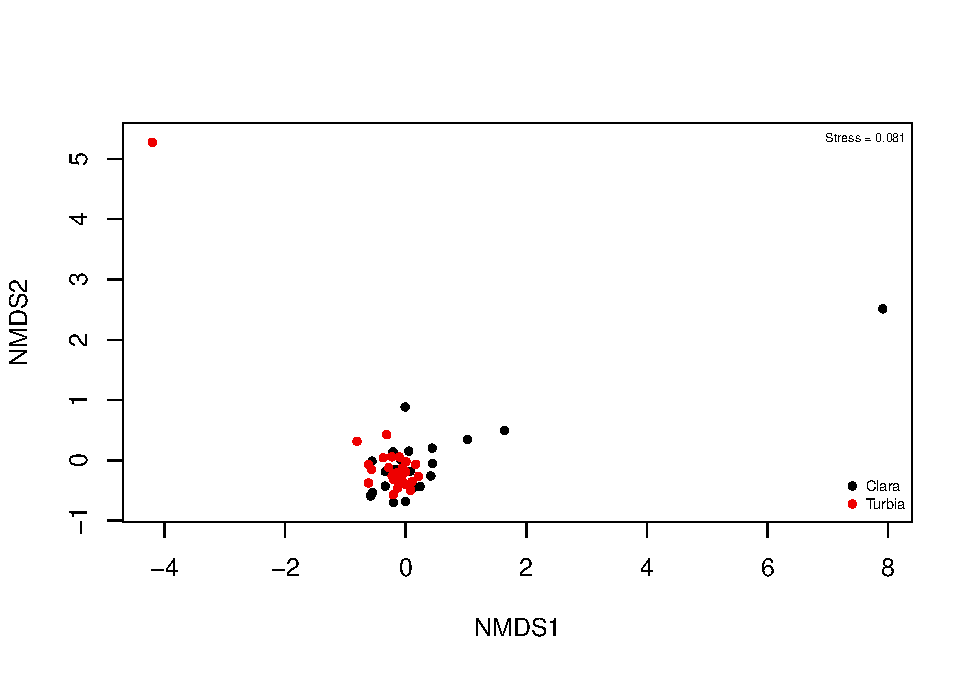
\includegraphics{04-multi1_b_files/figure-latex/unnamed-chunk-24-1.pdf}

El escalamiento es parecido al resultado del ACP, en donde se pueden observar que hay un solapamiento importante en el tipo de lagunas.

\hypertarget{permanova}{%
\section{PERMANOVA}\label{permanova}}

El análisis multivariante de permutaciones de la varianza o PerMANOVA, es una alternativa no paramétrica a la prueba de ANOVA multivariada. Es apropiado con conjuntos de múltiples variables que no cumples los supuestos, por ejemplo, el de normalidad. Además, se puede utilizar para datos muy sesgados, ordinales o cualitativos, y en datos de comunidades ecológicas, datos de comunidades microbiana o en datos genéticos. Su funcionamiento incluye una matriz de distancias construida a partir de cualquier medida de disimilitud. Este análisis se utiliza para comparar grupos de objetos y probar con la hipótesis nula de que los centroides y la dispersión de los grupos son equivalentes. Este análisis suele acompañar a los gráficos de ordenamiento tales como el NMDS.

\begin{Shaded}
\begin{Highlighting}[]
\NormalTok{res.perma }\OtherTok{\textless{}{-}} \FunctionTok{adonis2}\NormalTok{(dis.dist}\SpecialCharTok{\textasciitilde{}}\NormalTok{condicion, }\AttributeTok{method =} \StringTok{"euclidean"}\NormalTok{, }\AttributeTok{permutations =} \DecValTok{599}\NormalTok{)}
\NormalTok{res.perma}
\end{Highlighting}
\end{Shaded}

\begin{verbatim}
## Permutation test for adonis under reduced model
## Terms added sequentially (first to last)
## Permutation: free
## Number of permutations: 599
## 
## adonis2(formula = dis.dist ~ condicion, permutations = 599, method = "euclidean")
##           Df SumOfSqs      R2      F Pr(>F)  
## condicion  1    14.03 0.04009 2.0462   0.06 .
## Residual  49   335.97 0.95991                
## Total     50   350.00 1.00000                
## ---
## Signif. codes:  0 '***' 0.001 '**' 0.01 '*' 0.05 '.' 0.1 ' ' 1
\end{verbatim}

Para comparar los distintos grupos se pueden hacer analisis a posteriori, de comparaciones entre los grupos.

\begin{Shaded}
\begin{Highlighting}[]
\FunctionTok{library}\NormalTok{(pairwiseAdonis)}
\end{Highlighting}
\end{Shaded}

\begin{verbatim}
## Loading required package: cluster
\end{verbatim}

\begin{Shaded}
\begin{Highlighting}[]
\NormalTok{res.pos}\OtherTok{\textless{}{-}} \FunctionTok{pairwise.adonis}\NormalTok{(dis.dist, condicion, }\AttributeTok{sim.method =} \StringTok{"euclidean"}\NormalTok{, }\AttributeTok{p.adjust.m =} \StringTok{"bonferroni"}\NormalTok{)}
\NormalTok{res.pos}
\end{Highlighting}
\end{Shaded}

\begin{verbatim}
##             pairs Df SumsOfSqs  F.Model         R2 p.value p.adjusted sig
## 1 Clara vs Turbia  1  14.03004 2.046231 0.04008584   0.048      0.048   .
\end{verbatim}

\hypertarget{multi2}{%
\chapter{Análisis multivariados II}\label{multi2}}

\textbf{TECNICAS DE ORDENACION CANONICA}

\textbf{Maria Eugenia del R. Llames}\footnote{\href{mailto:mariaellames@intech.gov.ar}{\nolinkurl{mariaellames@intech.gov.ar}}}

Instituto Tecnológico de Chascomús (INTECH, UNSAM-CONICET), Escuela de Bio y Nanotecnologías (UNSAM)

\hypertarget{introducciuxf3n}{%
\section{INTRODUCCIÓN}\label{introducciuxf3n}}

\begin{quote}
El supuesto principal de cualquier técnica de ordenación es que los datos analizados son redundantes, es decir, contienen más variables (y dimensiones) de las necesarias para describir la información subyacente, y podemos reducir el número de estas dimensiones sin perder demasiada información. Por ejemplo, en el caso de los datos de composición de especies, algunas de las especies suelen ser ecológicamente similares (por ejemplo, especies que prefieren crecer en un hábitat húmedo en lugar de seco), lo que significa que el conjunto de datos contiene varias variables redundantes (especies) que cuentan la misma historia. O, para explicar la redundancia de otra manera, a partir de la presencia de una especie, a menudo podemos predecir la presencia de varias otras especies. En el caso de la ordenación aplicada en la matriz de variables ambientales, estas a menudo se correlacionan entre sí (por ejemplo, las mediciones del temperatura del agua a menudo se relacionan con las concentraciones de oxígeno disuelto), lo que también permite la reducción de la dimensión.
\end{quote}

\begin{quote}
Dado que el espacio multidimensional no es fácil de mostrar, describir o simplemente imaginar, vale la pena reducirlo a unas pocas dimensiones principales, conservando al máximo la información. Esto también significa que si las variables individuales son completamente independientes entre sí (por ejemplo, cada especie tiene preferencias completamente diferentes), entonces es probable que la ordenación no encuentre una reducción razonable del espacio multidimensional.
\end{quote}

\begin{quote}
Lo que hace el método de ordenación se puede formular de dos maneras alternativas:(i) busca gradientes en la composición de especies (representados generalmente por ejes de ordenación) e intenta explicar estos gradientes por variables ambientales; y/o (ii) busca la distribución de muestras en un espacio de ordenación reducido que refleje al máximo la disimilitud (= distancia) entre muestras en términos de su composición de especies.
\end{quote}

\begin{quote}
De acuerdo al apartado anterior (\textbf{Unidad 4}), las técnicas allí presentadas permiten el análisis de una única matriz de datos de forma tal de revelar su estructura a través de un grafo construido con un conjunto reducido de ejes ortogonales (\emph{i.e} independientes) Las variables externas que pueden estar influenciando esta estructura sólo podrán ser consideradas después del cómputo de la ordenación. De acuerdo con esta caracterísitica, se las conocen como ``técnicas de ordenación indirecta'' en donde uno deja que la matriz de datos exprese las relaciones entre objetos y variables sin restricción (``\emph{unconstrained analyses}''). Por lo tanto es una forma pasiva de análisis, y el usuario interpreta los resultados de la ordenación \emph{a posteriori}.
\end{quote}

\begin{quote}
Las técnicas de \textbf{ordenación canónica}, por el contrario, permiten asociar dos o más conjuntos de datos en el propio proceso de ordenación. Típicamente,en ecología, estas matrices la constituyen una matriz de datos biológicos, como por ejemplo, relevamiento de especies en diferentes sitios (matriz de ``respuesta'') y su matriz ambiental asociada (matriz ``explicativa'') (Figura 1).
\end{quote}

\textbf{Figura 1:} \emph{Esquema de las matrices utilizadas comúnmente en estudios ecológicos}

\begin{quote}
En este contexto, las técnicas de ordenación canónicas se engloban dentro de las ``técnicas de ordenación directa'' y permiten analizar patrones entre un conjunto de datos que están relacionadas con (o pueden ser interpretadas por) otro conjunto de datos, y/o probar formalmente hipótesis estadísticas sobre la importancia de estas relaciones. En otras palabras, las técnicas de ordenación canónica exploran explícitamente las relaciones entre dos matrices: una matriz de respuesta y una matriz explicativa y ambas matrices son utilizadas en la producción de la ordenación. Son análisis ``restringidos'' o ``\emph{constrained analyses}'' (Figura 2).
\end{quote}

\textbf{Figura 2:} \emph{Esquema de ``funcionamiento'' de las técnicas de ordenación canónicas.}

\hypertarget{la-luxf3gica-de-las-tuxe9cnicas-de-ordenaciuxf3n-restringida-o-canuxf3nica-constrained-anuxe1lisis-de-gradiente-directo}{%
\subsection{\texorpdfstring{LA LÓGICA DE LAS TÉCNICAS DE ORDENACIÓN RESTRINGIDA O CANÓNICA (``\emph{CONSTRAINED}'', ANÁLISIS DE GRADIENTE DIRECTO)}{LA LÓGICA DE LAS TÉCNICAS DE ORDENACIÓN RESTRINGIDA O CANÓNICA (``CONSTRAINED'', ANÁLISIS DE GRADIENTE DIRECTO)}}\label{la-luxf3gica-de-las-tuxe9cnicas-de-ordenaciuxf3n-restringida-o-canuxf3nica-constrained-anuxe1lisis-de-gradiente-directo}}

\begin{quote}
Los ejes de ordenación están limitados/restringidos por factores ambientales. Relaciona la composición de especies directamente con las variables ambientales y extrae la variación en la composición de especies que está directamente relacionada con el medio ambiente. Las variables ambientales ingresan directamente al algoritmo, y los ejes de ordenación restringidos corresponden a las direcciones de la variabilidad en los datos que se explica por estas variables ambientales. El método generalmente se usa como análisis confirmatorio, es decir, puede probar las hipótesis sobre la relación entre los factores ambientales en la composición de especies (a diferencia de la ordenación sin restricciones, que es exploratoria). Descompone la varianza total en los datos de composición de especies en una fracción explicada por variables ambientales (relacionadas con ejes de ordenación restringidos) y no explicada por variables ambientales (relacionadas con ejes de ordenación no restringidos). Ofrece varias oportunidades interesantes cuando se trata de variables explicativas: permite selección directa (la selección de variables ambientales importantes mediante la exclusión de aquellas que no son relevantes para la composición de especies), habilita la prueba de permutación de Monte Carlo (una prueba de significancia de la varianza explicada por factores ambientales) y permite el análisis de la partición de la varianza (partición de la varianza explicada por diferentes grupos de variables ambientales).
\end{quote}

\hypertarget{quuxe9-tipo-de-datos-de-composiciuxf3n-de-especies-se-utilizan-para-el-anuxe1lisis}{%
\subsection{¿Qué tipo de datos de composición de especies se utilizan para el análisis?}\label{quuxe9-tipo-de-datos-de-composiciuxf3n-de-especies-se-utilizan-para-el-anuxe1lisis}}

\begin{quote}
\hypertarget{a-muxe9todos-basados-en-datos-brutos-enfoque-cluxe1sico}{%
\subsubsection{(a) Métodos basados en datos brutos (enfoque clásico)}\label{a-muxe9todos-basados-en-datos-brutos-enfoque-cluxe1sico}}
\end{quote}

\begin{quote}
Métodos basados en el análisis de matrices crudas de muestras-especies con datos de abundancia o presencia/ausencia. Dentro de estos métodos, se reconocen tradicionalmente dos categorías, que se diferencian por la suposición de la respuesta de las especies a lo largo del gradiente ambiental:
\end{quote}

\begin{quote}
\begin{enumerate}
\def\labelenumi{\arabic{enumi}.}
\tightlist
\item
  \textbf{lineal} (Figura 3, panel izquierdo): supone que las especies responden linealmente a lo largo del gradiente ambiental, lo que podría ser cierto para datos ecológicos bastante homogéneos, y esto se da cuando donde los gradientes ecológicos considerados son bastante cortos;
\end{enumerate}
\end{quote}

\begin{quote}
2.\textbf{unimodal} (Figura 3, panel derecho): respuesta de la especie unimodalmente a lo largo del gradiente, con su punto óptimo en una determinada posición del gradiente; este modelo se acerca más a la realidad de los datos ecológicos y es más adecuado para conjuntos de datos heterogéneos (estructurados por un gradiente ecológico fuerte o largo, con un alto recambio de especies y muchos ceros en la matriz de especies), es decir, análisi de gradientes ambientales bastante largos.
\end{quote}

\textbf{Figura 3:} \emph{Supuesto de respuesta lineal (izquierda) frente a unimodal (derecha) del ``fitness''/abundancia de las especies a lo largo del medio ambiente.Fuente \url{https://www.davidzeleny.net/anadat-r/doku.php/en:ordination}}

\hypertarget{b-muxe9todos-aplicados-sobre-datos-transformados}{%
\subsubsection{(b) Métodos aplicados sobre datos transformados}\label{b-muxe9todos-aplicados-sobre-datos-transformados}}

\begin{quote}
Todos los métodos de ordenación tienen implícito un paso de cálculo de índices de distancia en su algoritmo. En algunos casos, tenemos la opción de indicarle al algoritmo qué índice utilizar (ejemplo: PCoA o NMDS), mientras que en otros el índice utilizado es fijo (ejemplo: PCA, RDA). Lo que tenemos que tener en cuenta es que, entre todos los índices posibles, existen índices ``\emph{simétricos}'' (incluyen el doble cero en el cálculo del índice), e índices ``\emph{asimétricos}'' (no incluyen al doble cero en el cálculo del índice). La utilización de índices símetricos en análisis de ordenación que suponen respuesta lineal pueden llevar a la paradoja de que dos sitios se ``ordenen cercanos'' en base a la ausencia de especies en ambos sitios (para más detalle sobre este punto, referirse al Capítulo 7 de libro ``Numerical Ecology'' de Legendre \& Legendre, 2012). En aquellos casos en que el modelo a aplicar es de respuesta lineal y se base en el cálculo de índices simétricos, se recomienda transformar los datos de composición de especies de forma tal de adecuar los datos ecológicos y evitar caer en la paradoja del doble-cero. En este sentido, Legendre y Gallagher (2001) detallan diversas transformaciones adecuadas para la aplicación de métodos de ordenación que asumen respuesta lineal.
\end{quote}

\hypertarget{c-muxe9todos-basados-en-la-distancia}{%
\subsubsection{(c) Métodos basados en la distancia}\label{c-muxe9todos-basados-en-la-distancia}}

\begin{quote}
Métodos que utilizan la matriz de distancias entre muestras medidas por coeficientes de distancia y que proyectan estas distancias en diagramas de ordenación de dos o más dimensiones. El método se conoce como db-RDA (RDA basado en la distancia) y consiste en una combinación de PCoA, aplicada en datos sin procesar utilizando una medida de distancia seleccionada, y RDA aplicada en los autovectores resultantes de PCoA (ver más abajo). Ofrece una alternativa a RDA (basada en distancias euclidianas) y al RDA basado en datos transformados (por ejemplo, transformados por Hellinger), con la libertad de elegir la medida de distancia adecuada para los datos investigados.
\end{quote}

\hypertarget{cuxf3mo-saber-si-debo-utilizar-un-muxe9todo-de-ordenaciuxf3n-de-respuesta-lineal-o-unimodal}{%
\subsection{¿Cómo saber si debo utilizar un método de ordenación de respuesta lineal o unimodal?}\label{cuxf3mo-saber-si-debo-utilizar-un-muxe9todo-de-ordenaciuxf3n-de-respuesta-lineal-o-unimodal}}

\begin{quote}
Para decidir si aplicar el método de ordenación de respuesta lineal o unimodal en los datos, podemos basarnos en la regla general introducida por Lepš \& Šmilauer (2003): primero, calcule DCA (``Detrended correspondence analysis''-análisis sin tendencia por segmentos) en sus datos y verifique la longitud del primer Eje del DCA (que está escalado en unidades de desviación estándar, S.D.). Una longitud del primer eje DCA \textgreater{} 4 S.D. indica un conjunto de datos heterogéneo en el que se deben utilizar métodos unimodales, mientras que la longitud \textless{} 3 S.D. indica un conjunto de datos homogéneo para el cual los métodos lineales son adecuados. En la zona gris entre 3 y 4 S.D., tanto los métodos lineales como los unimodales son adecuados. Sin embargo, tengan en cuenta que si bien \textbf{los métodos lineales no deben usarse para datos heterogéneos} (\emph{i.e.} para datos de respuesta unimodal), los métodos unimodales pueden ser usados para datos homogéneos, no obstante, los métodos lineales, en este caso, son más poderosos y deberían ser preferidos.
Alternativamente, si tus datos de composición de especies son heterogéneos, pero aún querés utilizar algún método de ordenación lineal (PCA, RDA), recordá trasnformar estos datos de composición de especies de forma tal de evitar el problema del doble-cero.
\end{quote}

\hypertarget{anuxe1lisis-de-redundancia-rda}{%
\subsection{\texorpdfstring{\textbf{ANÁLISIS DE REDUNDANCIA (RDA)}}{ANÁLISIS DE REDUNDANCIA (RDA)}}\label{anuxe1lisis-de-redundancia-rda}}

\begin{quote}
El RDA es un método que combina las técnicas de regresión lineal con el análisis de componentes principales (PCA). Por un lado, es una extensión directa del análisis de regresión múltiple para modelar la respuesta multivariada de datos. \emph{Redundancia} es sinónimo de ``variación explicada'' y se interpreta de la misma manera que como lo aprendieron en sus cursos introductorios de Estadísitica al estudiar los modelos de análisis univariados. El análisis se dice \emph{asimétrico} (\emph{i.e.} se establece una matriz de respuesta y una matriz explicativa), en donde la matriz ``Y'' (biológica) corresponde a la variable multidimensional de respuesta y ``X'' (o ``E'', de acuerdo a la Figura 1), corresponde a la matriz multidimensional de variables explicativas. Desde una perspectiva descriptiva, uno diría que la ordenación de ``Y'' está \emph{restringida} de forma tal que los vectores de ordenación resultantes son combinaciones lineales de las variables en ``X''.
\end{quote}

\begin{quote}
Por otro lado, RDA también puede verse como una extensión del análisis de componentes principales (PCA), porque los vectores de ordenación canónica que resultan constituyen combinaciones lineales de las variables de respuesta ``Y''. Esto significa que cada vector de ordenación es una proyección unidimensional de la distribución de los objetos en un espacio que conserva las distancias euclidianas entre ellos.
\end{quote}

\begin{quote}
Rápidamente, este método busca, en orden sucesivo, una serie de \emph{combinaciones lineales} de las \emph{variables explicativas} que \emph{mejor explican} la \emph{variación} de los datos de la matriz de \emph{variable respuesta}. Los \emph{ejes} definidos en el espacio a partir de la matriz de las variables explicativas son \emph{ortogonales} entre sí (\emph{i.e} independientes). RDA es por lo tanto un \emph{procedimiento de ordenación restringida}. La diferencia con la ordenación sin restricciones es importante: la matriz de variables explicativas condiciona los ``pesos'' (\emph{i.e.} autovalores, valores propios o \emph{eigenvalues}) y las direcciones de los ejes de ordenación. En RDA, uno puede decir verdaderamente que los ejes explican o modelan (en el sentido estadístico) la variación de la matriz respuesta o dependiente.
\end{quote}

\begin{quote}
Como resultado, la variación en la composición de especies se descompone en variación relacionada con variables ambientales (representadas por ejes restringidos/canónicos, autovectores o \emph{eigenvectors}) y no relacionada con variables ambientales (ejes no restringidos). El número total de ejes canónicos generdados corresponde a la cantidad \emph{min {[}p, m, n-1{]}}. Es decir, la cantidad de ejes será el número más bajo entre los parámetros \emph{p}, \emph{m}, y \emph{(n-1)}, talque \emph{(i)} la cantidad de ejes generados no puede exceder \emph{p} que es el tamaño del espacio de referencia de la matriz ``Y'' (\emph{i.e.} número de variables respuesta cosnideradas, de especies para nuestro caso); \emph{(ii)} no puede exceder \emph{m} que es el número de variables en X (cantidad de variables ambientales consideradas) y \emph{(iii)} no puede exceder (n -- 1), que es el número máximo de dimensiones requeridas para representar \emph{n} puntos (\emph{i.e.} sitios) en el espacio euclidiano. Finalmente, la significancia estadística del modelo de RDA (modelo global) y la de los ejes canónicos se pueden probar mediante análisis permutacionales (no paramétricos).
\end{quote}

\hypertarget{analicemos-estos-aspectos-a-travuxe9s-de-un-ejemplo-pruxe1ctico}{%
\subsection{Analicemos estos aspectos a través de un ejemplo práctico\ldots{}}\label{analicemos-estos-aspectos-a-travuxe9s-de-un-ejemplo-pruxe1ctico}}

\begin{quote}
Utilizaremos un set de datos del trabajo \emph{Bacterioplankton morphotypes structure and cytometric fingerprint rely on environmental conditions in a sub-Antarctic peatland} publicado en \emph{Hydrobiologia} (Quiroga \emph{et al.} 2017), disponibles en el \href{http://hdl.handle.net/11336/201811}{Repositorio Institucional} \href{http://hdl.handle.net/11336/201874}{CONICET Digital}. Para ello, descargar el set de datos \textbf{morpho\_biomass.csv} y \textbf{chem.csv} de \href{https://github.com/Limno-con-R/CILCAL2023/tree/main/datasets}{GitHub Limno-con-R/CILCAL2023}.
Guardar los archivos en una carpeta llamada \emph{data}, dentro del \textbf{Directorio de Trabajo} del \textbf{Proyecto} que creamos para esta Unidad (ver cómo hacerlo en la Unidad \ref{intro}). Finalmente, instalar los paquetes como se indica en la Unidad \ref{intro}. Luego, cargarlos en la sesión.
\end{quote}

\hypertarget{rda-utilizando-el-paquete-vegan-oksanen-et-al.-2007}{%
\subsection{\texorpdfstring{RDA utilizando el paquete \textbf{vegan} (Oksanen \emph{et al.}, 2007)}{RDA utilizando el paquete vegan (Oksanen et al., 2007)}}\label{rda-utilizando-el-paquete-vegan-oksanen-et-al.-2007}}

\begin{Shaded}
\begin{Highlighting}[]
\FunctionTok{library}\NormalTok{ (vegan)}
\end{Highlighting}
\end{Shaded}

\begin{verbatim}
## Warning: package 'vegan' was built under R version 4.2.3
\end{verbatim}

\begin{verbatim}
## Loading required package: permute
\end{verbatim}

\begin{verbatim}
## Loading required package: lattice
\end{verbatim}

\begin{verbatim}
## This is vegan 2.6-4
\end{verbatim}

\begin{Shaded}
\begin{Highlighting}[]
\NormalTok{data\_biomass }\OtherTok{\textless{}{-}}\FunctionTok{read.csv}\NormalTok{(}\StringTok{"./data/morpho\_biomass.csv"}\NormalTok{,}\AttributeTok{row.names=}\DecValTok{1}\NormalTok{) }\CommentTok{\# biomasa [pgC/mL]}
\NormalTok{biomass }\OtherTok{\textless{}{-}}\NormalTok{data\_biomass[,}\DecValTok{4}\SpecialCharTok{:}\DecValTok{9}\NormalTok{] }\CommentTok{\#selecciono solo los datos de biomasa de los diferentes morfotipos de la matriz de datos biologicos}
\NormalTok{bio.trans }\OtherTok{\textless{}{-}}\FunctionTok{log10}\NormalTok{(biomass}\SpecialCharTok{+}\DecValTok{1}\NormalTok{) }\CommentTok{\# transformacion log10(x+1). Esta transformación se utiliza para estabilizar varianzas. Si tengo un grupo extremadamente dominante y otros menos representados, es una buena opción. Más detalle sobre transformaciones pueden encontrar en la biblio del curso. }
\end{Highlighting}
\end{Shaded}

\begin{Shaded}
\begin{Highlighting}[]
\CommentTok{\# Cómputo del DCA para verificar la longitud del gradiente}
\CommentTok{\#{-}{-}{-}{-}}

\NormalTok{vare.dca }\OtherTok{\textless{}{-}} \FunctionTok{decorana}\NormalTok{(bio.trans)}
\NormalTok{vare.dca}
\end{Highlighting}
\end{Shaded}

\begin{verbatim}
## 
## Call:
## decorana(veg = bio.trans) 
## 
## Detrended correspondence analysis with 26 segments.
## Rescaling of axes with 4 iterations.
## Total inertia (scaled Chi-square): 0.109 
## 
##                         DCA1     DCA2      DCA3      DCA4
## Eigenvalues          0.07139 0.005130 0.0020470 0.0012492
## Additive Eigenvalues 0.07139 0.008798 0.0117827 0.0154503
## Decorana values      0.10595 0.001355 0.0005076 0.0002615
## Axis lengths         0.60193 0.239784 0.1647616 0.1281498
\end{verbatim}

\begin{quote}
La última línea de la primer columna (DCA1) indica \emph{Axis lengths= 0.60193}. Ese valor corresponde a la longitud del primer eje de ordenamiento del DCA, expresado en unidades de desvio estándar (S.D.) de recambio de especies. Un gradiente mayor a 4 S.D. indica que algunas especies presentan respuesta unimodal. En el caso de nuestr ejemplo, la longitud del gradiente es \textless{} 4, indicando un gradiente homogéneo o corto y, por lo tanto, el modelo de respuesta lineal es el adecuado para aplicar.
Porcedemos, entonces, al modelado a través de un RDA:
\end{quote}

\begin{Shaded}
\begin{Highlighting}[]
\CommentTok{\# RDA}
\CommentTok{\#{-}{-}{-}{-}}
\CommentTok{\# Seleccion de variables explicativas}
\NormalTok{ambiental }\OtherTok{\textless{}{-}}\FunctionTok{read.csv}\NormalTok{(}\StringTok{"./data/chem.csv"}\NormalTok{, }\AttributeTok{row.names=}\DecValTok{1}\NormalTok{) }\CommentTok{\#cargo las variables ambientales}
\NormalTok{env }\OtherTok{\textless{}{-}}\NormalTok{ ambiental[,}\FunctionTok{c}\NormalTok{(}\DecValTok{4}\SpecialCharTok{:}\DecValTok{5}\NormalTok{,}\DecValTok{7}\SpecialCharTok{:}\DecValTok{15}\NormalTok{)] }\CommentTok{\# saco una de ellas: "DO" (oxígeno disuelto) ya que tiene datos faltantes (NAs) y el modelo no corre con variables que tengan datos faltantes}
\end{Highlighting}
\end{Shaded}

\begin{quote}
Hasta acá, hemos (i) verificado el tipo de respuesta en nuestros datos de composición de especie para elegir el modelo adecuado y (ii) preparamos los datos de composición y de datos ambientales para modelar.
Además del tipo de respuesta, otro requisito necesario es la ``multinormalidad'' de los datos de la matriz ambiental. En el siguiente paso, lo que vamos a hacer es chequear que este supuesto se cumpla:
\end{quote}

\begin{verbatim}
##  [1]  0.7514272 -0.8963630  0.3566289  0.4353447  0.6865369  0.1131861
##  [7]  1.5255447  0.7839304  0.4965284  0.3858427 -0.2629160
\end{verbatim}

\begin{verbatim}
## [1] 0.854080999478208 0.186705671286224 <NA>             
## Levels: 0.854080999478208 0.186705671286224
\end{verbatim}

\begin{quote}
En este caso, elegimos analizar la asimetría de los datos (``\emph{skewness}'') a través del estudio de la significancia de los coeficiente de asimetría y curtosis multivariado de Mardia. Para la normalidad multivariada, los valores \emph{p} de las estadísticas de asimetría y curtosis deben ser superiores a 0,05. Si el tamaño de la muestra es inferior a 20, se debe utilizar \emph{p.value.small} como valor significativo de asimetría en lugar de \emph{p.value.skew}.
\end{quote}

\begin{quote}
Con los supuestos del modelo revisados y comprobados, avanzamos con la aplicación del modelo a los datos. En el caso del paquete \textbf{vegan}, permite el cálculo de una RDA de dos maneras diferentes. La sintaxis más simple es listar los nombres de los marcos de datos involucrados separados por comas:
\end{quote}

\begin{Shaded}
\begin{Highlighting}[]
\NormalTok{simpleRDA }\OtherTok{\textless{}{-}} \FunctionTok{rda}\NormalTok{(bio.trans, env)}
\end{Highlighting}
\end{Shaded}

\begin{quote}
Esta manera, si bien es sencilla, tiene algunas limitaciones. Su principal inconveniente es que no permite incluir variables cualitativas en la matriz explicativa. Por lo tanto, en todas las aplicaciones excepto en las más simples, es mejor usar la interfaz de la fórmula:
\end{quote}

\begin{Shaded}
\begin{Highlighting}[]
\NormalTok{biomass.rda}\OtherTok{\textless{}{-}}\FunctionTok{rda}\NormalTok{(bio.trans }\SpecialCharTok{\textasciitilde{}}\NormalTok{ ., }\AttributeTok{data=}\NormalTok{ env, }\AttributeTok{scale=}\ConstantTok{TRUE}\NormalTok{ )}\CommentTok{\#dado que las variables \#ambietnales son dimensionalmente heterogéneas, debemos escalar los datos a una \#distribución normal, de media cero y varianza 1 ( N\textasciitilde{}(0,1))}
\CommentTok{\#Observación: Observá el atajo (.) para indicarle a la función que use todas las \#variables presentes en la matriz env}
\FunctionTok{summary}\NormalTok{ (biomass.rda)}
\end{Highlighting}
\end{Shaded}

\begin{verbatim}
## 
## Call:
## rda(formula = bio.trans ~ pH + EC + TH + DOC + DIN + TN + DRP +      TP + a440 + SUVA254 + E2_E3, data = env, scale = TRUE) 
## 
## Partitioning of correlations:
##               Inertia Proportion
## Total           6.000     1.0000
## Constrained     4.657     0.7762
## Unconstrained   1.343     0.2238
## 
## Eigenvalues, and their contribution to the correlations 
## 
## Importance of components:
##                         RDA1   RDA2    RDA3    RDA4     RDA5     RDA6    PC1
## Eigenvalue            3.1710 0.8844 0.33988 0.21332 0.033907 0.014628 0.6473
## Proportion Explained  0.5285 0.1474 0.05665 0.03555 0.005651 0.002438 0.1079
## Cumulative Proportion 0.5285 0.6759 0.73256 0.76811 0.773762 0.776200 0.8841
##                           PC2     PC3      PC4      PC5       PC6
## Eigenvalue            0.36127 0.23664 0.058178 0.035203 0.0042519
## Proportion Explained  0.06021 0.03944 0.009696 0.005867 0.0007087
## Cumulative Proportion 0.94429 0.98373 0.993424 0.999291 1.0000000
## 
## Accumulated constrained eigenvalues
## Importance of components:
##                         RDA1   RDA2    RDA3   RDA4     RDA5     RDA6
## Eigenvalue            3.1710 0.8844 0.33988 0.2133 0.033907 0.014628
## Proportion Explained  0.6809 0.1899 0.07298 0.0458 0.007281 0.003141
## Cumulative Proportion 0.6809 0.8708 0.94377 0.9896 0.996859 1.000000
## 
## Scaling 2 for species and site scores
## * Species are scaled proportional to eigenvalues
## * Sites are unscaled: weighted dispersion equal on all dimensions
## * General scaling constant of scores:  3.26758 
## 
## 
## Species scores
## 
##          RDA1    RDA2    RDA3     RDA4     RDA5      RDA6
## Fil    0.1640  0.9800  0.1229 -0.36682  0.01563  0.006191
## Lrods  1.0807  0.1722  0.1353  0.21391  0.04241  0.124300
## Vibrio 1.0330  0.1990 -0.3880  0.10220  0.14806 -0.061658
## Lcocci 1.0518 -0.2601  0.5923 -0.01995  0.02843 -0.065814
## Srods  1.1491  0.2899 -0.1576  0.12975 -0.18794 -0.032996
## Scocci 0.9769 -0.6264 -0.2126 -0.41426 -0.01565  0.036324
## 
## 
## Site scores (weighted sums of species scores)
## 
##         RDA1     RDA2      RDA3     RDA4      RDA5     RDA6
## 1O -0.315023 -0.01150 -0.135348  1.83690  1.989508  2.36638
## 2O -1.007735  1.21914  0.282566  0.40541  2.088730  1.04932
## 3O -1.484836  1.11482  1.265037 -1.32407 -1.594090 -0.24504
## 4O -0.600298  0.02235 -0.719724  1.50242 -0.090550  1.60198
## 5O -1.158091 -0.80220  1.212587 -0.40025 -1.467472 -0.72606
## 1D  0.125647 -0.12541 -0.241248  1.54171  0.244519 -2.25780
## 2D  0.503364 -0.50115  0.265594  0.84928 -1.481579  0.48143
## 3D  0.571223 -0.93323  0.477569 -0.33140 -3.801358 -1.22805
## 4D  1.440168  1.09255 -0.009618 -1.21473 -1.730754  2.44805
## 5D  1.110690 -0.83129  1.491267  0.91641  5.229787 -0.65145
## 1F -0.004785  0.97072  0.213935 -0.49315  0.297806 -4.20914
## 2F  0.243819 -0.95176 -0.343644 -0.70321 -1.449543 -1.28073
## 3F -0.145507  0.29996  0.622884 -2.30409 -2.203613  4.03065
## 4F  0.955108  1.20742  0.102013  0.23464  0.302300  0.83304
## 5F  0.660170 -0.47342 -0.933551  0.65107  0.249799 -0.36565
## 1A  0.284992  1.49562 -0.243656  0.11548  0.300082  0.24773
## 2A -0.126578 -0.94884  0.028396 -0.58969  1.471159  0.03331
## 3A  0.450376 -0.60836 -1.317999  0.08787  0.958064 -0.96982
## 4A -1.273194 -0.62696 -1.942517 -0.96279  0.691910 -1.54544
## 5A -0.229511 -0.60848 -0.074542  0.18221 -0.004706  0.38729
## 
## 
## Site constraints (linear combinations of constraining variables)
## 
##         RDA1     RDA2     RDA3     RDA4     RDA5     RDA6
## 1O -0.666050 -0.03263 -0.20456  0.67067  0.30973  1.13043
## 2O -0.589321  0.88879 -0.19113  1.06969  0.83522  0.07651
## 3O -1.147534  0.65602  0.97820 -0.32919 -0.63364  0.64437
## 4O -0.541377  0.06784  0.30905  0.83005 -0.34576  0.49226
## 5O -1.367806 -0.60884  0.89670  0.09781  0.20458  0.29427
## 1D  0.009829  0.05750 -0.08803  1.53774  0.90167 -1.38061
## 2D -0.051073  0.14523  0.39871  0.09523 -1.36220  0.16740
## 3D  0.791745 -0.67157  0.49123  0.56383 -1.01736 -1.11073
## 4D  1.402806  0.76775 -0.20109 -0.26664  1.09996  0.76278
## 5D  0.750646 -0.79242  1.44929 -0.54727  0.84634 -0.33252
## 1F  0.188119  0.86592  0.35285 -0.64724  0.05688 -0.77830
## 2F  0.543423 -0.25688 -0.09422 -0.22587  0.52622  1.29148
## 3F -0.217915 -0.65881  0.07894 -1.19060  0.10541 -0.28021
## 4F  1.014708  0.75753 -0.24087  0.08763 -1.74999  0.36433
## 5F  0.318650 -0.94261 -1.09939  0.29612  0.09228  0.31852
## 1A -0.073515  1.77741 -0.15026 -0.49096  0.29268 -0.96792
## 2A  0.288515 -0.54700  0.59304 -0.89605  0.35509  0.05141
## 3A  0.419385 -0.12031 -1.15996 -0.05880 -0.12945  0.59023
## 4A -1.205438 -0.29740 -1.70082 -1.29957 -0.08222 -0.77949
## 5A  0.132203 -1.05551 -0.41768  0.70342 -0.30544 -0.55421
## 
## 
## Biplot scores for constraining variables
## 
##             RDA1     RDA2     RDA3      RDA4     RDA5      RDA6
## pH       0.24581  0.67115 -0.41787 -0.003153  0.13921 -0.281524
## EC       0.62762 -0.23182 -0.44280 -0.411541 -0.22997 -0.241235
## TH      -0.01424  0.32740 -0.10029  0.266745 -0.02467 -0.130398
## DOC      0.39463 -0.34017  0.01318 -0.137529 -0.02881 -0.475663
## DIN     -0.25130 -0.14701 -0.40052  0.175035  0.16676  0.188011
## TN       0.53545 -0.12080  0.01779 -0.644442  0.25086 -0.011189
## DRP     -0.17603  0.32493  0.29212 -0.201619  0.04890  0.152063
## TP       0.16442 -0.03934 -0.66674 -0.027193 -0.13282 -0.005328
## a440     0.03653 -0.48845 -0.66818 -0.233564 -0.24154 -0.272376
## SUVA254  0.13008 -0.29171 -0.27511  0.019930 -0.30331  0.359999
## E2_E3   -0.17459 -0.17869 -0.06789  0.162049  0.09327 -0.451209
\end{verbatim}

\begin{Shaded}
\begin{Highlighting}[]
\CommentTok{\# Coeficientes canónicos }
\FunctionTok{coef}\NormalTok{(biomass.rda)}
\end{Highlighting}
\end{Shaded}

\begin{verbatim}
##                  RDA1          RDA2          RDA3          RDA4          RDA5
## pH       2.152488e-02  1.592068e-01 -1.762663e-02  6.615200e-02 -6.710379e-02
## EC       2.531088e-02  7.981753e-04 -1.679251e-02 -1.075705e-02 -1.256239e-02
## TH      -6.176966e-03  1.827047e-02 -6.753879e-03 -1.236731e-02 -9.362529e-03
## DOC      3.715987e-02  1.313701e-02  5.364947e-02  4.154162e-02 -7.030470e-02
## DIN     -4.111146e-04 -1.983296e-04 -4.529877e-03  1.006686e-04  4.049021e-03
## TN       7.788896e-06 -1.510186e-05 -8.793536e-06 -4.098084e-05  9.646049e-05
## DRP     -5.590659e-03  8.149917e-03  1.649684e-03 -8.282799e-03 -9.950571e-03
## TP       2.128018e-03  1.801153e-04 -1.587443e-03  2.700815e-03  2.960609e-03
## a440    -1.459099e-01  2.398457e-03 -1.904511e-02 -1.356861e-01 -1.003461e-01
## SUVA254  4.905131e-02 -9.475625e-03  2.433850e-02  7.493413e-02 -8.659162e-02
## E2_E3    4.729434e-02 -2.018131e-01 -1.164860e-01  2.563431e-01  5.309020e-01
##                  RDA6
## pH      -2.039089e-01
## EC       2.933565e-02
## TH       7.262698e-03
## DOC     -5.807067e-02
## DIN      6.838714e-03
## TN       1.385058e-05
## DRP      1.061373e-03
## TP       6.682286e-04
## a440    -8.433608e-02
## SUVA254  3.630886e-02
## E2_E3   -8.524522e-02
\end{verbatim}

\begin{Shaded}
\begin{Highlighting}[]
\DocumentationTok{\#\# Test Global para el RDA con todas las variables}
\end{Highlighting}
\end{Shaded}

\begin{Shaded}
\begin{Highlighting}[]
\FunctionTok{anova}\NormalTok{(biomass.rda, }\AttributeTok{permutations =} \FunctionTok{how}\NormalTok{(}\AttributeTok{nperm =} \DecValTok{999}\NormalTok{))}\CommentTok{\#nada tiene que ver este análisis \#con el tradicional "ANOVA"de la estadística univariada...}
\end{Highlighting}
\end{Shaded}

\begin{verbatim}
## Permutation test for rda under reduced model
## Permutation: free
## Number of permutations: 999
## 
## Model: rda(formula = bio.trans ~ pH + EC + TH + DOC + DIN + TN + DRP + TP + a440 + SUVA254 + E2_E3, data = env, scale = TRUE)
##          Df Variance      F Pr(>F)   
## Model    11   4.6572 2.5224  0.007 **
## Residual  8   1.3428                 
## ---
## Signif. codes:  0 '***' 0.001 '**' 0.01 '*' 0.05 '.' 0.1 ' ' 1
\end{verbatim}

\begin{Shaded}
\begin{Highlighting}[]
\CommentTok{\#R\^{}2}
\NormalTok{(R2 }\OtherTok{\textless{}{-}} \FunctionTok{RsquareAdj}\NormalTok{(biomass.rda)}\SpecialCharTok{$}\NormalTok{r.squared)}\CommentTok{\# 0.78}
\end{Highlighting}
\end{Shaded}

\begin{verbatim}
## [1] 0.7762
\end{verbatim}

\begin{Shaded}
\begin{Highlighting}[]
\CommentTok{\#el R\^{}2, al igual que ocurre en la regresión múltiple, está "inflado" por la cantidad \#de variables incluidas en el mdoelo, es decir, aumenta al incluir más variables, \#independientemente de que exista una relación o nó entre ellas y la matriz respuesta. \#Además, la acumulación de variables explicativas infla la cantidad aparente de \#varianza explicada como consecuencia de correlaciones aleatorias entre variables. Este \#problema se puede solucionar ajustando el R\^{}2}


\CommentTok{\# R\^{}2 ajustado (penalizado por la cantidad de variables incluidas en le modelo, mide la \#cantidad de variación explicada "sin sesgo") }
\NormalTok{(R2adj }\OtherTok{\textless{}{-}} \FunctionTok{RsquareAdj}\NormalTok{(biomass.rda)}\SpecialCharTok{$}\NormalTok{adj.r.squared)}
\end{Highlighting}
\end{Shaded}

\begin{verbatim}
## [1] 0.4684749
\end{verbatim}

\begin{Shaded}
\begin{Highlighting}[]
\CommentTok{\#0.47}
\end{Highlighting}
\end{Shaded}

\begin{quote}
Expliquemos un poco esta salida\ldots{}
En primer lugar, se revisa la prueba global del modelo utilizando todas las variables explicativas (resultado de la función \emph{anova}). Si, y solo si, la prueba global es significativa, se puede proceder con la selección de variables (más abajo).
La salida anterior porporciona información útil: ``\emph{Inertia}'' (Inercia) es otro nombre para variación o varianza en este caso. ``\emph{Total}'' se refiere a la varianza total, ``\emph{Constrained}'' (Restringida) se refiere a la cantidad de varianza explicada por las variables explicativas, ``\emph{Unconstrainded}'' (Sin restricciones) se refiere a la varianza residual. Restringido + Sin restricciones = Total. Se deriva, además, un estadístico R\textsuperscript{2} que se interpreta de manera similar al R\textsuperscript{2} de regresión: representa la variación explicada por el modelo en relación a la varianza total (Restringido/Total).Los autovalores se muestran tanto para los ejes restringidos como para los no restringidos. En este contexto, estos autovalores indican qué con cantidad de varianza contribuye cada uno de los ejes.
\end{quote}

\begin{quote}
Podemos graficar el resultado de nuestro modelo (con todas las variables explicativas) para tener una idea de qué variables se correlacionan con especies a lo largo de qué ejes.
\end{quote}

\begin{Shaded}
\begin{Highlighting}[]
\FunctionTok{ordiplot}\NormalTok{(biomass.rda, }\AttributeTok{scaling =} \DecValTok{1}\NormalTok{, }\AttributeTok{type =} \StringTok{"text"}\NormalTok{)}
\end{Highlighting}
\end{Shaded}

\includegraphics{05-multi2_files/figure-latex/unnamed-chunk-8-1.pdf}

\textbf{Figura 4:} El ``\emph{escalado}'' 1 refleja en el gráfico las similitudes entre objetos en la matriz de respuesta. Es decir, los sitios (en negro) que están más cerca entre sí tienen comunidades más similares. Las especies que están más juntas ocupan más sitios en común.

\begin{Shaded}
\begin{Highlighting}[]
\FunctionTok{ordiplot}\NormalTok{(biomass.rda, }\AttributeTok{scaling =} \DecValTok{2}\NormalTok{, }\AttributeTok{type =} \StringTok{"text"}\NormalTok{)}
\end{Highlighting}
\end{Shaded}

\includegraphics{05-multi2_files/figure-latex/unnamed-chunk-9-1.pdf}

\textbf{Figura 5:} El ``\emph{escalado}'' 2 muestra los efectos de las variables explicativas. Las flechas más largas significan que esta variable impulsa fuertemente la variación en la matriz de la comunidad. Las flechas que apuntan en direcciones opuestas tienen una relación negativa. Las flechas que apuntan en la misma dirección tienen una relación positiva. Cuanto más superpuestas las flechas, más correlacionadas resultan esas variables (ya sea positiva o negtivamente).

\hypertarget{seleccionando-las-variables-explicativas-relevantes}{%
\subsection{Seleccionando las variables explicativas relevantes}\label{seleccionando-las-variables-explicativas-relevantes}}

\begin{quote}
Si queremos simplificar este modelo, podemos realizar una selección hacia adelante (\emph{forward}, van ingresando de a una por vez al modelo), o hacia atrás (\emph{backward}, inicia con todas las variables involucradas y va eliminando de a una), o paso a paso (\emph{stepwise}, proceso iterativo de inclusión y exclusión de variables). Estos tipos de selecciones nos ayudan a seleccionar variables que son estadísticamente importantes. Sin embargo, es importante notar que seleccionar variables de relevancia ecológica es mucho más importante que realizar la selección de variables ``estadísticamente significativas''. Si una variable relevante desde el punto de vista ecológico no se selecciona ``estadísticamente'', esto no significa que deba eliminarse del RDA.
\end{quote}

\begin{Shaded}
\begin{Highlighting}[]
\CommentTok{\# Forward selection of variables:}
\NormalTok{fwd.sel }\OtherTok{\textless{}{-}} \FunctionTok{ordistep}\NormalTok{(}\FunctionTok{rda}\NormalTok{(bio.trans }\SpecialCharTok{\textasciitilde{}} \DecValTok{1}\NormalTok{, }\AttributeTok{data =}\NormalTok{ env, }\AttributeTok{scale=} \ConstantTok{TRUE}\NormalTok{), }\CommentTok{\# modelo mínimo con una sola variable incluída}
               \AttributeTok{scope =} \FunctionTok{formula}\NormalTok{(biomass.rda), }\CommentTok{\#modelo "de máxima", con todas las variables incluidas, completo}
               \AttributeTok{direction =} \StringTok{"forward"}\NormalTok{,}
               \AttributeTok{R2scope =} \ConstantTok{TRUE}\NormalTok{, }\CommentTok{\# no puede sobrepasar el R\^{}2 del modelo completo}
               \AttributeTok{pstep =} \DecValTok{1000}\NormalTok{,}
               \AttributeTok{trace =} \ConstantTok{TRUE}\NormalTok{) }\CommentTok{\# cambiar a FALSE para no ver todo el proceso de selección}
\end{Highlighting}
\end{Shaded}

\begin{verbatim}
## 
## Start: bio.trans ~ 1 
## 
##           Df    AIC      F Pr(>F)   
## + EC       1 33.486 5.4886  0.005 **
## + TN       1 35.111 3.6559  0.035 * 
## + DOC      1 36.689 2.0134  0.105   
## + pH       1 36.512 2.1912  0.120   
## + a440     1 37.495 1.2229  0.270   
## + DIN      1 37.847 0.8874  0.415   
## + DRP      1 38.029 0.7166  0.470   
## + TP       1 37.997 0.7466  0.525   
## + SUVA254  1 38.270 0.4923  0.695   
## + E2_E3    1 38.353 0.4154  0.745   
## + TH       1 38.425 0.3496  0.795   
## ---
## Signif. codes:  0 '***' 0.001 '**' 0.01 '*' 0.05 '.' 0.1 ' ' 1
## 
## Step: bio.trans ~ EC 
## 
##           Df    AIC      F Pr(>F)  
## + a440     1 30.718 4.5770  0.015 *
## + pH       1 32.870 2.3759  0.085 .
## + E2_E3    1 34.177 1.1501  0.350  
## + TN       1 34.291 1.0469  0.390  
## + DIN      1 34.608 0.7632  0.440  
## + TP       1 34.803 0.5910  0.625  
## + DRP      1 34.851 0.5485  0.625  
## + DOC      1 34.986 0.4307  0.705  
## + TH       1 34.873 0.5294  0.745  
## + SUVA254  1 35.170 0.2709  0.910  
## ---
## Signif. codes:  0 '***' 0.001 '**' 0.01 '*' 0.05 '.' 0.1 ' ' 1
## 
## Step: bio.trans ~ EC + a440 
## 
##           Df    AIC      F Pr(>F)  
## + pH       1 30.098 2.2393  0.095 .
## + TP       1 30.590 1.7964  0.160  
## + TN       1 31.422 1.0710  0.360  
## + DOC      1 31.460 1.0392  0.365  
## + DRP      1 31.766 0.7802  0.530  
## + SUVA254  1 31.840 0.7185  0.570  
## + TH       1 32.114 0.4904  0.690  
## + E2_E3    1 32.045 0.5477  0.720  
## + DIN      1 32.500 0.1756  0.970  
## ---
## Signif. codes:  0 '***' 0.001 '**' 0.01 '*' 0.05 '.' 0.1 ' ' 1
\end{verbatim}

\begin{quote}
Para evitar la sobreestimación de la varianza explicada, la selección de variables debe realizarse con dos criterios de parada: (1) el nivel de significación alfa habitual y (2) el coeficiente de determinación múltiple ajustado (R\textsuperscript{2}adj.) calculado utilizando todas las variables explicativas. Cuando la selección hacia adelante identifica una variable que hace que uno u otro criterio supere el umbral fijado, se rechaza esa variable y se detiene el procedimiento (referirse a Blanchet, F. G., Legendre, P., \& Borcard, D. 2008. \emph{Forward selection of explanatory variables}. Ecology, 89(9): 2623-2632, para más detalles).
\end{quote}

\begin{quote}
Qué variables son retenidas por la selección \emph{forward}?
\end{quote}

\begin{Shaded}
\begin{Highlighting}[]
\NormalTok{fwd.sel}\SpecialCharTok{$}\NormalTok{call}
\end{Highlighting}
\end{Shaded}

\begin{verbatim}
## rda(formula = bio.trans ~ EC + a440, data = env, scale = TRUE)
\end{verbatim}

\begin{quote}
Cuál es el valor del R\textsuperscript{2} ajustado de este modelo?
\end{quote}

\begin{Shaded}
\begin{Highlighting}[]
\CommentTok{\# Escribir el modelo}
\NormalTok{biomass.rda.signif }\OtherTok{\textless{}{-}} \FunctionTok{rda}\NormalTok{(bio.trans }\SpecialCharTok{\textasciitilde{}}\NormalTok{ EC }\SpecialCharTok{+}\NormalTok{ a440, }\AttributeTok{data =}\NormalTok{ env, }\AttributeTok{scale=} \ConstantTok{TRUE}\NormalTok{)}


\FunctionTok{RsquareAdj}\NormalTok{(biomass.rda.signif)}
\end{Highlighting}
\end{Shaded}

\begin{verbatim}
## $r.squared
## [1] 0.3962273
## 
## $adj.r.squared
## [1] 0.3251952
\end{verbatim}

\begin{quote}
Tests de significación
\end{quote}

\begin{Shaded}
\begin{Highlighting}[]
\FunctionTok{anova.cca}\NormalTok{(biomass.rda.signif, }\AttributeTok{step =} \DecValTok{1000}\NormalTok{) }\CommentTok{\#Significación global del modelo final}
\end{Highlighting}
\end{Shaded}

\begin{verbatim}
## Permutation test for rda under reduced model
## Permutation: free
## Number of permutations: 999
## 
## Model: rda(formula = bio.trans ~ EC + a440, data = env, scale = TRUE)
##          Df Variance      F Pr(>F)   
## Model     2   2.3774 5.5781  0.002 **
## Residual 17   3.6226                 
## ---
## Signif. codes:  0 '***' 0.001 '**' 0.01 '*' 0.05 '.' 0.1 ' ' 1
\end{verbatim}

\begin{Shaded}
\begin{Highlighting}[]
\FunctionTok{anova.cca}\NormalTok{(biomass.rda.signif, }\AttributeTok{step =} \DecValTok{1000}\NormalTok{, }\AttributeTok{by =} \StringTok{"term"}\NormalTok{) }\CommentTok{\#significación de variables }
\end{Highlighting}
\end{Shaded}

\begin{verbatim}
## Permutation test for rda under reduced model
## Terms added sequentially (first to last)
## Permutation: free
## Number of permutations: 999
## 
## Model: rda(formula = bio.trans ~ EC + a440, data = env, scale = TRUE)
##          Df Variance      F Pr(>F)   
## EC        1   1.4020 6.5793  0.002 **
## a440      1   0.9753 4.5770  0.011 * 
## Residual 17   3.6226                 
## ---
## Signif. codes:  0 '***' 0.001 '**' 0.01 '*' 0.05 '.' 0.1 ' ' 1
\end{verbatim}

\begin{Shaded}
\begin{Highlighting}[]
\FunctionTok{anova.cca}\NormalTok{(biomass.rda.signif, }\AttributeTok{step =} \DecValTok{1000}\NormalTok{, }\AttributeTok{by =} \StringTok{"axis"}\NormalTok{) }\CommentTok{\#significación de los ejes}
\end{Highlighting}
\end{Shaded}

\begin{verbatim}
## Permutation test for rda under reduced model
## Forward tests for axes
## Permutation: free
## Number of permutations: 999
## 
## Model: rda(formula = bio.trans ~ EC + a440, data = env, scale = TRUE)
##          Df Variance      F Pr(>F)   
## RDA1      1   1.9986 9.3787  0.002 **
## RDA2      1   0.3788 1.7776  0.128   
## Residual 17   3.6226                 
## ---
## Signif. codes:  0 '***' 0.001 '**' 0.01 '*' 0.05 '.' 0.1 ' ' 1
\end{verbatim}

\begin{quote}
Colinealidad entre variables explicativas
\end{quote}

\begin{Shaded}
\begin{Highlighting}[]
\FunctionTok{vif.cca}\NormalTok{(biomass.rda.signif) }\CommentTok{\#Sii vif ("variable inflation factor") \textless{}5 no hay colinealidad}
\end{Highlighting}
\end{Shaded}

\begin{verbatim}
##       EC     a440 
## 1.693375 1.693375
\end{verbatim}

\hypertarget{rda-basado-en-matriz-de-distancia-distance-based-rda-db-rda}{%
\subsection{RDA basado en matriz de distancia (``Distance-based RDA'', db-RDA)}\label{rda-basado-en-matriz-de-distancia-distance-based-rda-db-rda}}

\begin{quote}
La diferencia en el análisis entre RDA y dbRDA es simplemente el paso de expresar una matriz de disimilitud no euclidiana en un espacio euclidiano. ¿Les suena familiar?\ldots{} Sí! eso es exactamente lo que hace un PCoA.
Los datos de especies crudos, sin procesar, se trasnforman primero en una matriz de disimilitud utilizando alguna métrica de disimilitud seleccionada, y con esta matriz se modela un PCoA. La matriz resultante de \emph{scores} de sitios sobre todos los ejes de ordenación de PCoA se usa luego en RDA junto con las variables explicativas. El beneficio de dbRDA es que se puede aplicar cualquier métrica de distancia a los datos (es decir, no solo euclidiana como en RDA, Hellinger (o algunas otras) como en tbRDA o chi-cuadrado como en CCA). Se debe tener cuidado y evitar los autovalores negativos obtenidos en el PCoA, que se omitirían de los análisis. Para que ellos no ocurra, la solución es usar solo distancias métricas (euclidianas), o aplicar una transformación a la matriz de distancia de forma tal de convertir esa distancia ``no métrica'' en una métrica (por ejemplo, la transformación de raíz cuadrada aplicada a la matriz de distancia obtenida por Bray-Curtis), o usar algunas de las correcciones propuestas en las diferentes funciones.
Notas:
1. Si se aplica dbRDA a una matriz de distancia euclidiana, el dbRDA resulta idéntico a RDA.
2. Si no se proporcionan variables explicativas, un dbRDA resulta idéntico a un PCoA
(porque el primer paso da como resultado un PCoA regular y el segundo paso no tiene sentido).
Estos pasos son bastante simples de realizar y se pueden ejecutar uno por uno en R con unas pocas líneas de código. Sin embargo, \textbf{vegan} propone la función \textbf{capscale()} para este análisis. Esta función permite el trazado directo de las puntuaciones medias ponderadas de las especies si el usuario proporciona la matriz de especies en el argumento \emph{com}.
\end{quote}

\begin{Shaded}
\begin{Highlighting}[]
\CommentTok{\#El primer paso es decidir qué medida de distancia usar. Una forma en que podemos hacer \#esto es observando las correlaciones entre los índices de disimilitud y la separación \#de gradiente; cuanto mayor sea el valor, mejor.}

\FunctionTok{rankindex}\NormalTok{(env, biomass, }\AttributeTok{indices =} \FunctionTok{c}\NormalTok{(}\StringTok{"euc"}\NormalTok{, }\StringTok{"man"}\NormalTok{, }\StringTok{"gow"}\NormalTok{, }\StringTok{"bra"}\NormalTok{, }\StringTok{"kul"}\NormalTok{), }\AttributeTok{stepacross=} \ConstantTok{FALSE}\NormalTok{, }\AttributeTok{method =} \StringTok{"spearman"}\NormalTok{)}
\end{Highlighting}
\end{Shaded}

\begin{verbatim}
##       euc       man       gow       bra       kul 
## 0.2327555 0.2591706 0.3040157 0.3376863 0.3214870
\end{verbatim}

\begin{quote}
La distancia de Bray Curtis parece ser el mejor índice para aplicar.
\end{quote}

\begin{Shaded}
\begin{Highlighting}[]
\CommentTok{\# 1. capscale() en base a datos crudos (sitos x especies)}
\NormalTok{bray.env.cap}\OtherTok{\textless{}{-}} \FunctionTok{capscale}\NormalTok{ (biomass }\SpecialCharTok{\textasciitilde{}} \DecValTok{1}\NormalTok{, env, }\AttributeTok{add =} \StringTok{"lingoes"}\NormalTok{ )}\CommentTok{\#modelo mínimo}
\NormalTok{bray.env.cap.all }\OtherTok{\textless{}{-}} \FunctionTok{capscale}\NormalTok{(biomass }\SpecialCharTok{\textasciitilde{}}\NormalTok{ . , env, }\AttributeTok{add =} \StringTok{"lingoes"}\NormalTok{)}\CommentTok{\# modelo completo}
\CommentTok{\# Existen dos maneras de evitar autovalores negativos: una es agregando una constante \#al análisis en el argumento "add" o tomando los valores de similitud transformados por \#raíz cuadrada (argumento sqrt.dist= TRUE). Más detalle en help (capscale)}

\NormalTok{fwd.sel.dbRDA}\OtherTok{\textless{}{-}}\FunctionTok{ordistep}\NormalTok{ (bray.env.cap, }\AttributeTok{scope =} \FunctionTok{formula}\NormalTok{ (bray.env.cap.all), }\AttributeTok{direction =} \StringTok{"forward"}\NormalTok{, }\AttributeTok{R2scope =} \ConstantTok{TRUE}\NormalTok{, }\CommentTok{\# no puede sobrepasar el R\^{}2 del modelo completo}
\AttributeTok{pstep =} \DecValTok{1000}\NormalTok{,}
\AttributeTok{trace =} \ConstantTok{TRUE}\NormalTok{)}
\end{Highlighting}
\end{Shaded}

\begin{verbatim}
## 
## Start: biomass ~ 1 
## 
##           Df    AIC      F Pr(>F)   
## + EC       1 435.62 7.3760  0.005 **
## + TN       1 436.35 6.4767  0.010 **
## + DOC      1 439.94 2.4469  0.130   
## + a440     1 440.76 1.6257  0.225   
## + TP       1 441.11 1.2859  0.305   
## + TH       1 441.34 1.0725  0.315   
## + DIN      1 441.51 0.9092  0.325   
## + SUVA254  1 441.40 1.0155  0.365   
## + E2_E3    1 441.53 0.8848  0.415   
## + pH       1 441.68 0.7432  0.440   
## + DRP      1 442.18 0.2880  0.730   
## ---
## Signif. codes:  0 '***' 0.001 '**' 0.01 '*' 0.05 '.' 0.1 ' ' 1
## 
## Step: biomass ~ EC 
## 
##           Df    AIC      F Pr(>F)  
## + a440     1 433.14 4.2685  0.020 *
## + TN       1 435.40 1.9954  0.110  
## + E2_E3    1 435.03 2.3593  0.120  
## + pH       1 435.57 1.8349  0.140  
## + TP       1 436.22 1.2399  0.280  
## + SUVA254  1 436.60 0.8973  0.430  
## + DIN      1 436.64 0.8577  0.475  
## + DOC      1 436.87 0.6540  0.545  
## + TH       1 437.12 0.4337  0.735  
## + DRP      1 437.50 0.1099  0.925  
## ---
## Signif. codes:  0 '***' 0.001 '**' 0.01 '*' 0.05 '.' 0.1 ' ' 1
## 
## Step: biomass ~ EC + a440 
## 
##           Df    AIC      F Pr(>F)  
## + pH       1 431.31 3.3846  0.045 *
## + TN       1 432.60 2.1715  0.100 .
## + E2_E3    1 433.25 1.5858  0.240  
## + DOC      1 433.79 1.1182  0.310  
## + SUVA254  1 434.40 0.6032  0.540  
## + TP       1 434.29 0.6956  0.570  
## + TH       1 434.31 0.6796  0.605  
## + DRP      1 434.72 0.3418  0.805  
## + DIN      1 434.90 0.1953  0.900  
## ---
## Signif. codes:  0 '***' 0.001 '**' 0.01 '*' 0.05 '.' 0.1 ' ' 1
## 
## Step: biomass ~ EC + a440 + pH 
## 
##           Df    AIC      F Pr(>F)
## + E2_E3    1 430.27 2.4564  0.115
## + TN       1 431.11 1.7398  0.150
## + TP       1 431.80 1.1744  0.320
## + DRP      1 432.24 0.8201  0.375
## + SUVA254  1 432.73 0.4406  0.715
## + DOC      1 432.71 0.4525  0.750
## + DIN      1 432.94 0.2786  0.845
## + TH       1 433.05 0.1947  0.895
\end{verbatim}

\begin{Shaded}
\begin{Highlighting}[]
\FunctionTok{ordiplot}\NormalTok{(bray.env.cap.all, }\AttributeTok{scaling =} \DecValTok{2}\NormalTok{, }\AttributeTok{type =} \StringTok{"text"}\NormalTok{)}
\end{Highlighting}
\end{Shaded}

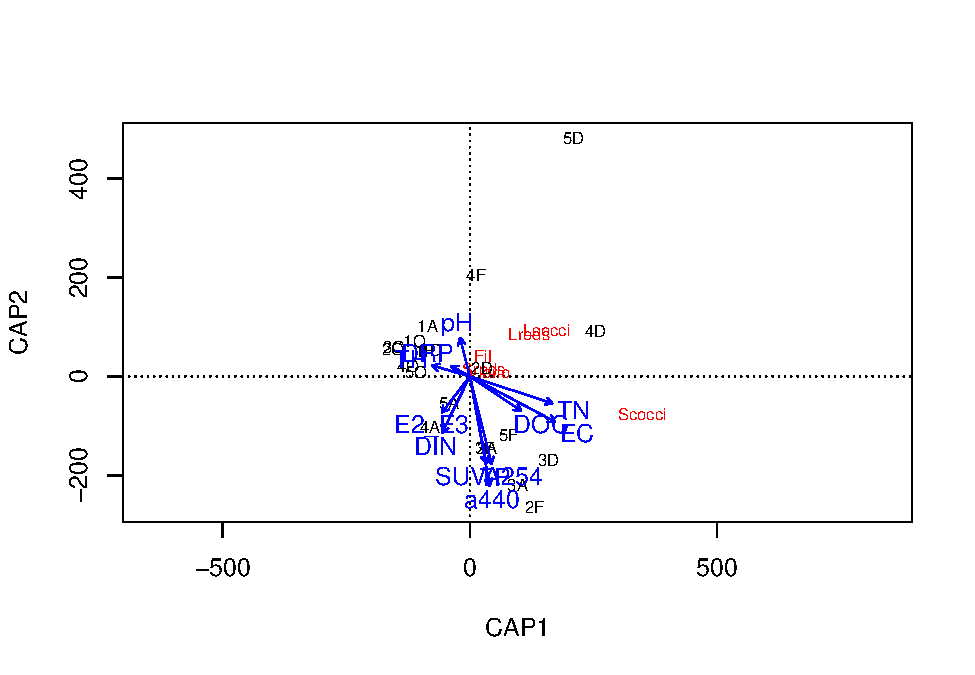
\includegraphics{05-multi2_files/figure-latex/unnamed-chunk-19-1.pdf}

\textbf{Figura 6:} Ordenamiento obtenido a partir del dbRDA en base a la distancia de Bray Curtis. Escalamiento tipo 2.

\begin{quote}
Qué variables son retenidas por la selección \emph{forward}?
\end{quote}

\begin{Shaded}
\begin{Highlighting}[]
\NormalTok{fwd.sel.dbRDA}\SpecialCharTok{$}\NormalTok{call}
\end{Highlighting}
\end{Shaded}

\begin{verbatim}
## capscale(formula = biomass ~ EC + a440 + pH, data = env, add = "lingoes")
\end{verbatim}

\begin{quote}
Cuál es el valor del R\textsuperscript{2} ajustado de este modelo?
\end{quote}

\begin{Shaded}
\begin{Highlighting}[]
\CommentTok{\# Escribir el modelo}
\NormalTok{biomass.dbrda.signif }\OtherTok{\textless{}{-}} \FunctionTok{capscale}\NormalTok{(}\AttributeTok{formula =}\NormalTok{ biomass }\SpecialCharTok{\textasciitilde{}}\NormalTok{ EC }\SpecialCharTok{+}\NormalTok{ a440 }\SpecialCharTok{+}\NormalTok{ pH, }\AttributeTok{data =}\NormalTok{ env, }\AttributeTok{add =} \StringTok{"lingoes"}\NormalTok{)}

\FunctionTok{RsquareAdj}\NormalTok{(biomass.dbrda.signif)}
\end{Highlighting}
\end{Shaded}

\begin{verbatim}
## $r.squared
## [1] 0.5320242
## 
## $adj.r.squared
## [1] 0.4442787
\end{verbatim}

\begin{quote}
Test de significación
\end{quote}

\begin{Shaded}
\begin{Highlighting}[]
\FunctionTok{anova.cca}\NormalTok{(biomass.dbrda.signif, }\AttributeTok{step =} \DecValTok{1000}\NormalTok{) }\CommentTok{\#Significación global del modelo final}
\end{Highlighting}
\end{Shaded}

\begin{verbatim}
## Permutation test for capscale under reduced model
## Permutation: free
## Number of permutations: 999
## 
## Model: capscale(formula = biomass ~ EC + a440 + pH, data = env, add = "lingoes")
##          Df   Variance      F Pr(>F)    
## Model     3 1861913203 6.0633  0.001 ***
## Residual 16 1637764593                  
## ---
## Signif. codes:  0 '***' 0.001 '**' 0.01 '*' 0.05 '.' 0.1 ' ' 1
\end{verbatim}

\begin{Shaded}
\begin{Highlighting}[]
\FunctionTok{anova.cca}\NormalTok{(biomass.dbrda.signif, }\AttributeTok{step =} \DecValTok{1000}\NormalTok{, }\AttributeTok{by =} \StringTok{"term"}\NormalTok{) }\CommentTok{\#significación de variables }
\end{Highlighting}
\end{Shaded}

\begin{verbatim}
## Permutation test for capscale under reduced model
## Terms added sequentially (first to last)
## Permutation: free
## Number of permutations: 999
## 
## Model: capscale(formula = biomass ~ EC + a440 + pH, data = env, add = "lingoes")
##          Df   Variance      F Pr(>F)    
## EC        1 1017246043 9.9379  0.001 ***
## a440      1  498217165 4.8673  0.019 *  
## pH        1  346449995 3.3846  0.052 .  
## Residual 16 1637764593                  
## ---
## Signif. codes:  0 '***' 0.001 '**' 0.01 '*' 0.05 '.' 0.1 ' ' 1
\end{verbatim}

\begin{Shaded}
\begin{Highlighting}[]
\FunctionTok{anova.cca}\NormalTok{(biomass.dbrda.signif, }\AttributeTok{step =} \DecValTok{1000}\NormalTok{, }\AttributeTok{by =} \StringTok{"axis"}\NormalTok{) }\CommentTok{\#significación de los ejes}
\end{Highlighting}
\end{Shaded}

\begin{verbatim}
## Permutation test for capscale under reduced model
## Forward tests for axes
## Permutation: free
## Number of permutations: 999
## 
## Model: capscale(formula = biomass ~ EC + a440 + pH, data = env, add = "lingoes")
##          Df   Variance       F Pr(>F)   
## CAP1      1 1503918383 14.6924  0.005 **
## CAP2      1  278096049  2.7168  0.163   
## CAP3      1   79898771  0.7806  0.512   
## Residual 16 1637764593                  
## ---
## Signif. codes:  0 '***' 0.001 '**' 0.01 '*' 0.05 '.' 0.1 ' ' 1
\end{verbatim}

\begin{quote}
Colinealidad entre variables explicativas
\end{quote}

\begin{Shaded}
\begin{Highlighting}[]
\FunctionTok{vif.cca}\NormalTok{(biomass.dbrda.signif) }\CommentTok{\#Sii vif ("variable inflation factor") \textless{}5 no hay colinealidad}
\end{Highlighting}
\end{Shaded}

\begin{verbatim}
##       EC     a440       pH 
## 1.932725 1.873615 1.153775
\end{verbatim}

\begin{quote}
Existe otra manera de calcular dbRDA que fue propuesta por McArdle y Anderson (2001). Este método alternativo ejecuta el análisis directamente sobre la matriz de similitud de respuesta sin tener que pasar por un PCoA. Esta forma alternativa es proporcionada en el paqueta \textbf{vegan} en la fucnión \textbf{dbrda()}.
\end{quote}

\begin{Shaded}
\begin{Highlighting}[]
\CommentTok{\# dbRDA}
\CommentTok{\#{-}{-}{-}{-}{-}{-}}
\CommentTok{\# generar la matriz de distancia}
\NormalTok{biomass.dist }\OtherTok{\textless{}{-}} \FunctionTok{vegdist}\NormalTok{(biomass, }\AttributeTok{method=}\StringTok{"bray"}\NormalTok{) }\CommentTok{\# bray curtis}
\end{Highlighting}
\end{Shaded}

\begin{Shaded}
\begin{Highlighting}[]
\CommentTok{\# Modelado}
\NormalTok{dbrda}\FloatTok{.0} \OtherTok{\textless{}{-}} \FunctionTok{dbrda}\NormalTok{(biomass.dist }\SpecialCharTok{\textasciitilde{}} \DecValTok{1}\NormalTok{, env, }\AttributeTok{add=}\ConstantTok{TRUE}\NormalTok{)}\CommentTok{\#modelo mínimo}
\NormalTok{dbrda.all }\OtherTok{\textless{}{-}} \FunctionTok{dbrda}\NormalTok{(biomass.dist }\SpecialCharTok{\textasciitilde{}}\NormalTok{ ., env, }\AttributeTok{add=}\ConstantTok{TRUE}\NormalTok{)}\CommentTok{\#modelo completo}
\NormalTok{fwd.sel.dbRDA2}\OtherTok{\textless{}{-}}\FunctionTok{ordistep}\NormalTok{ (dbrda}\FloatTok{.0}\NormalTok{, }\AttributeTok{scope =} \FunctionTok{formula}\NormalTok{ (dbrda.all), }\AttributeTok{add=}\ConstantTok{TRUE}\NormalTok{)}
\end{Highlighting}
\end{Shaded}

\begin{verbatim}
## 
## Start: biomass.dist ~ 1 
## 
##           Df    AIC      F Pr(>F)   
## + EC       1 18.715 6.6542  0.005 **
## + TN       1 20.679 4.3484  0.005 **
## + DOC      1 22.618 2.2839  0.065 . 
## + a440     1 22.817 2.0827  0.065 . 
## + DRP      1 23.525 1.3845  0.210   
## + DIN      1 23.810 1.1098  0.345   
## + SUVA254  1 24.037 0.8944  0.410   
## + TH       1 24.081 0.8529  0.485   
## + TP       1 24.087 0.8474  0.485   
## + pH       1 24.092 0.8425  0.505   
## + E2_E3    1 24.382 0.5712  0.720   
## ---
## Signif. codes:  0 '***' 0.001 '**' 0.01 '*' 0.05 '.' 0.1 ' ' 1
## 
## Step: biomass.dist ~ EC 
## 
##      Df    AIC      F Pr(>F)   
## - EC  1 23.007 6.6542  0.005 **
## ---
## Signif. codes:  0 '***' 0.001 '**' 0.01 '*' 0.05 '.' 0.1 ' ' 1
## 
##           Df    AIC      F Pr(>F)  
## + a440     1 18.018 2.4546  0.020 *
## + DRP      1 19.089 1.4399  0.135  
## + pH       1 19.078 1.4506  0.150  
## + TN       1 19.061 1.4660  0.195  
## + E2_E3    1 19.284 1.2616  0.235  
## + DIN      1 19.478 1.0851  0.395  
## + DOC      1 19.703 0.8828  0.500  
## + TH       1 19.807 0.7900  0.615  
## + TP       1 19.883 0.7230  0.660  
## + SUVA254  1 20.175 0.4660  0.970  
## ---
## Signif. codes:  0 '***' 0.001 '**' 0.01 '*' 0.05 '.' 0.1 ' ' 1
## 
## Step: biomass.dist ~ EC + a440 
## 
##        Df    AIC      F Pr(>F)   
## - a440  1 18.715 2.4546  0.050 * 
## - EC    1 22.817 6.8831  0.005 **
## ---
## Signif. codes:  0 '***' 0.001 '**' 0.01 '*' 0.05 '.' 0.1 ' ' 1
## 
##           Df    AIC      F Pr(>F)  
## + pH       1 17.824 1.8552  0.045 *
## + TN       1 18.218 1.5069  0.090 .
## + TP       1 18.175 1.5445  0.125  
## + DRP      1 18.257 1.4724  0.135  
## + TH       1 18.889 0.9289  0.435  
## + DOC      1 18.935 0.8905  0.545  
## + E2_E3    1 18.937 0.8890  0.555  
## + SUVA254  1 19.014 0.8242  0.565  
## + DIN      1 19.423 0.4831  0.950  
## ---
## Signif. codes:  0 '***' 0.001 '**' 0.01 '*' 0.05 '.' 0.1 ' ' 1
## 
## Step: biomass.dist ~ EC + a440 + pH 
## 
##        Df    AIC      F Pr(>F)   
## - pH    1 18.018 1.8552  0.110   
## - a440  1 19.078 2.8267  0.025 * 
## - EC    1 23.836 7.8833  0.005 **
## ---
## Signif. codes:  0 '***' 0.001 '**' 0.01 '*' 0.05 '.' 0.1 ' ' 1
## 
## Step: biomass.dist ~ EC + a440 
## 
##           Df    AIC      F Pr(>F)  
## + pH       1 17.824 1.8552  0.055 .
## + TN       1 18.218 1.5069  0.085 .
## + TP       1 18.175 1.5445  0.140  
## + DRP      1 18.257 1.4724  0.170  
## + TH       1 18.889 0.9289  0.460  
## + DOC      1 18.935 0.8905  0.555  
## + E2_E3    1 18.937 0.8890  0.575  
## + SUVA254  1 19.014 0.8242  0.675  
## + DIN      1 19.423 0.4831  0.940  
## ---
## Signif. codes:  0 '***' 0.001 '**' 0.01 '*' 0.05 '.' 0.1 ' ' 1
## 
##        Df    AIC      F Pr(>F)   
## - a440  1 18.715 2.4546  0.045 * 
## - EC    1 22.817 6.8831  0.005 **
## ---
## Signif. codes:  0 '***' 0.001 '**' 0.01 '*' 0.05 '.' 0.1 ' ' 1
## 
##           Df    AIC      F Pr(>F)  
## + pH       1 17.824 1.8552  0.035 *
## + TP       1 18.175 1.5445  0.095 .
## + TN       1 18.218 1.5069  0.125  
## + DRP      1 18.257 1.4724  0.145  
## + E2_E3    1 18.937 0.8890  0.470  
## + TH       1 18.889 0.9289  0.520  
## + DOC      1 18.935 0.8905  0.585  
## + SUVA254  1 19.014 0.8242  0.605  
## + DIN      1 19.423 0.4831  0.960  
## ---
## Signif. codes:  0 '***' 0.001 '**' 0.01 '*' 0.05 '.' 0.1 ' ' 1
## 
## Step: biomass.dist ~ EC + a440 + pH 
## 
##        Df    AIC      F Pr(>F)   
## - pH    1 18.018 1.8552  0.075 . 
## - a440  1 19.078 2.8267  0.030 * 
## - EC    1 23.836 7.8833  0.005 **
## ---
## Signif. codes:  0 '***' 0.001 '**' 0.01 '*' 0.05 '.' 0.1 ' ' 1
## 
##           Df    AIC      F Pr(>F)  
## + TP       1 17.506 1.8428  0.050 *
## + DRP      1 17.560 1.7980  0.065 .
## + TN       1 18.201 1.2684  0.210  
## + E2_E3    1 18.352 1.1453  0.370  
## + TH       1 18.613 0.9364  0.465  
## + DOC      1 18.917 0.6956  0.775  
## + SUVA254  1 18.944 0.6748  0.830  
## + DIN      1 19.177 0.4931  0.920  
## ---
## Signif. codes:  0 '***' 0.001 '**' 0.01 '*' 0.05 '.' 0.1 ' ' 1
## 
## Step: biomass.dist ~ EC + a440 + pH + TP 
## 
##        Df    AIC      F Pr(>F)   
## - TP    1 17.824 1.8428  0.095 . 
## - pH    1 18.175 2.1410  0.090 . 
## - a440  1 20.167 3.9360  0.015 * 
## - EC    1 24.511 8.5293  0.005 **
## ---
## Signif. codes:  0 '***' 0.001 '**' 0.01 '*' 0.05 '.' 0.1 ' ' 1
## 
##           Df    AIC      F Pr(>F)  
## + DRP      1 16.699 2.1102  0.040 *
## + E2_E3    1 17.878 1.1876  0.210  
## + TN       1 17.810 1.2392  0.250  
## + TH       1 18.280 0.8858  0.515  
## + DOC      1 18.389 0.8046  0.570  
## + SUVA254  1 18.726 0.5574  0.905  
## + DIN      1 18.762 0.5308  0.915  
## ---
## Signif. codes:  0 '***' 0.001 '**' 0.01 '*' 0.05 '.' 0.1 ' ' 1
## 
## Step: biomass.dist ~ EC + a440 + pH + TP + DRP 
## 
##        Df    AIC      F Pr(>F)   
## - DRP   1 17.506 2.1102  0.105   
## - TP    1 17.560 2.1532  0.100 . 
## - pH    1 18.515 2.9436  0.025 * 
## - a440  1 20.239 4.4688  0.010 **
## - EC    1 25.377 9.8785  0.005 **
## ---
## Signif. codes:  0 '***' 0.001 '**' 0.01 '*' 0.05 '.' 0.1 ' ' 1
## 
## Step: biomass.dist ~ EC + a440 + pH + TP 
## 
##           Df    AIC      F Pr(>F)  
## + DRP      1 16.699 2.1102  0.030 *
## + TN       1 17.810 1.2392  0.225  
## + E2_E3    1 17.878 1.1876  0.310  
## + TH       1 18.280 0.8858  0.515  
## + DOC      1 18.389 0.8046  0.630  
## + SUVA254  1 18.726 0.5574  0.910  
## + DIN      1 18.762 0.5308  0.935  
## ---
## Signif. codes:  0 '***' 0.001 '**' 0.01 '*' 0.05 '.' 0.1 ' ' 1
## 
## Step: biomass.dist ~ EC + a440 + pH + TP + DRP 
## 
##        Df    AIC      F Pr(>F)   
## - TP    1 17.560 2.1532  0.060 . 
## - DRP   1 17.506 2.1102  0.045 * 
## - pH    1 18.515 2.9436  0.025 * 
## - a440  1 20.239 4.4688  0.005 **
## - EC    1 25.377 9.8785  0.005 **
## ---
## Signif. codes:  0 '***' 0.001 '**' 0.01 '*' 0.05 '.' 0.1 ' ' 1
## 
##           Df    AIC      F Pr(>F)  
## + TN       1 16.046 1.8438  0.060 .
## + DOC      1 17.329 0.9210  0.535  
## + TH       1 17.397 0.8739  0.580  
## + E2_E3    1 17.506 0.7989  0.655  
## + SUVA254  1 17.757 0.6268  0.850  
## + DIN      1 17.854 0.5611  0.880  
## ---
## Signif. codes:  0 '***' 0.001 '**' 0.01 '*' 0.05 '.' 0.1 ' ' 1
\end{verbatim}

\begin{Shaded}
\begin{Highlighting}[]
\FunctionTok{summary}\NormalTok{(fwd.sel.dbRDA2)}
\end{Highlighting}
\end{Shaded}

\begin{verbatim}
## 
## Call:
## dbrda(formula = biomass.dist ~ EC + a440 + pH + TP + DRP, data = env,      add = TRUE) 
## 
## Partitioning of Lingoes adjusted squared Bray distance:
##               Inertia Proportion
## Total           3.009     1.0000
## Constrained     1.678     0.5575
## Unconstrained   1.331     0.4425
## 
## Eigenvalues, and their contribution to the Lingoes adjusted squared Bray distance 
## 
## Importance of components:
##                       dbRDA1 dbRDA2  dbRDA3  dbRDA4  dbRDA5   MDS1    MDS2
## Eigenvalue            1.0703 0.3221 0.12877 0.09009 0.06647 0.3678 0.20959
## Proportion Explained  0.3557 0.1070 0.04279 0.02994 0.02209 0.1222 0.06965
## Cumulative Proportion 0.3557 0.4627 0.50552 0.53546 0.55755 0.6798 0.74943
##                          MDS3    MDS4    MDS5    MDS6    MDS7    MDS8    MDS9
## Eigenvalue            0.17540 0.10549 0.08807 0.07393 0.05742 0.05189 0.04836
## Proportion Explained  0.05829 0.03506 0.02927 0.02457 0.01908 0.01724 0.01607
## Cumulative Proportion 0.80772 0.84277 0.87204 0.89661 0.91569 0.93293 0.94900
##                         MDS10   MDS11   MDS12    MDS13    MDS14
## Eigenvalue            0.04089 0.03853 0.03519 0.024559 0.014278
## Proportion Explained  0.01359 0.01280 0.01170 0.008162 0.004745
## Cumulative Proportion 0.96259 0.97540 0.98709 0.995255 1.000000
## 
## Accumulated constrained eigenvalues
## Importance of components:
##                       dbRDA1 dbRDA2  dbRDA3  dbRDA4  dbRDA5
## Eigenvalue             1.070 0.3221 0.12877 0.09009 0.06647
## Proportion Explained   0.638 0.1920 0.07676 0.05370 0.03962
## Cumulative Proportion  0.638 0.8299 0.90668 0.96038 1.00000
## 
## Scaling 2 for species and site scores
## * Species are scaled proportional to eigenvalues
## * Sites are unscaled: weighted dispersion equal on all dimensions
## * General scaling constant of scores:  2.749779 
## 
## 
## Site scores (weighted sums of species scores)
## 
##      dbRDA1    dbRDA2   dbRDA3   dbRDA4   dbRDA5     MDS1
## 1O -0.66177 -0.132828 -0.08959 -0.66141  1.08241  0.23164
## 2O -1.12361 -0.703321 -1.12959 -1.15553  0.66718 -0.97955
## 3O -1.13289 -1.392541 -0.48992  1.51413 -1.18819 -1.25738
## 4O -0.88509  0.095203 -0.34704 -0.87820  0.51330 -0.40484
## 5O -0.81340  0.487815 -0.01471 -0.10775 -0.92183  1.03532
## 1D -0.28776  0.321297  0.95037 -0.48981  0.43639  0.52258
## 2D  0.41611  0.245248  0.26170 -0.25717 -0.46966  0.12984
## 3D  0.79080 -0.007137 -0.89970 -0.18287  0.62830 -0.01169
## 4D  1.02607 -1.341192  0.32315 -0.12623  0.09512 -0.01968
## 5D  0.96387 -0.678324 -0.50040 -0.61642 -1.60054  0.64482
## 1F -0.43323  0.171314  0.66604 -0.26967 -0.23443 -0.33023
## 2F  0.63887  0.263552 -0.79425 -0.06902  0.11445  0.42287
## 3F  0.27916  0.612592 -0.80159  1.03340 -0.55649  0.12495
## 4F  0.48902 -0.439799  1.88244 -0.63326 -0.70495 -0.18254
## 5F  0.60574  0.111096 -0.03600  0.60760  1.25946  0.33757
## 1A -0.35564 -0.587072  1.33692  1.26054  0.35992  0.92485
## 2A  0.34551  0.615936 -0.82057  0.17808 -0.29773  0.01335
## 3A  0.58476  0.223384 -0.22519  0.83457  1.18538  0.46487
## 4A -0.34673  1.242182  0.54157  0.10483 -0.22698 -1.07174
## 5A -0.09978  0.892597  0.18637 -0.08582 -0.14112 -0.59501
## 
## 
## Site constraints (linear combinations of constraining variables)
## 
##      dbRDA1   dbRDA2   dbRDA3    dbRDA4   dbRDA5     MDS1
## 1O -0.53307 -0.40397 -0.57997 -0.103417  0.37580  0.23164
## 2O -0.84955 -0.43534 -0.20140 -0.911766  0.87484 -0.97955
## 3O -0.59128 -1.09759 -0.64176  1.235130 -0.74002 -1.25738
## 4O -0.64595 -0.01218 -0.32465 -0.651934  0.09808 -0.40484
## 5O -1.38536  0.54304 -0.39510 -0.803274 -0.21869  1.03532
## 1D -0.39777  0.14876  0.88386 -0.291199 -0.44145  0.52258
## 2D  0.48687  0.06101 -0.42604 -0.364645 -0.70724  0.12984
## 3D  0.77718 -0.01113 -0.72868 -0.007326  0.67824 -0.01169
## 4D  0.92707 -1.26462  0.82674 -0.760836 -0.03088 -0.01968
## 5D  0.57971 -0.30129 -0.51144 -0.091981 -1.05526  0.64482
## 1F -0.05628  0.11848  0.47350 -0.186501 -0.38489 -0.33023
## 2F  0.30217 -0.07984 -0.15611 -0.121069 -0.30798  0.42287
## 3F  0.10634  0.98806 -0.31458  0.527650 -0.55853  0.12495
## 4F  0.60245 -0.18492  0.92179 -0.586995  0.21340 -0.18254
## 5F  0.55139  0.29392 -0.65811  0.233307  1.37109  0.33757
## 1A -0.78958 -0.63560  1.21030  1.323061  0.40709  0.92485
## 2A  0.32949 -0.10949 -0.41455  0.362815 -0.22740  0.01335
## 3A  0.34484  0.19814 -0.09886  0.788439  0.86578  0.46487
## 4A  0.01653  1.22298  0.84255  0.246673  0.28781 -1.07174
## 5A  0.22480  0.96158  0.29250  0.163868 -0.49980 -0.59501
## 
## 
## Biplot scores for constraining variables
## 
##        dbRDA1   dbRDA2   dbRDA3   dbRDA4   dbRDA5 MDS1
## EC    0.84744  0.25745  0.27261  0.36853  0.07372    0
## a440  0.33292  0.71473 -0.02621  0.39707  0.46903    0
## pH   -0.01327 -0.19504  0.96606 -0.03142  0.16592    0
## TP    0.25049  0.07963 -0.03589  0.41833  0.86870    0
## DRP  -0.22871 -0.55583 -0.22802  0.76265 -0.07146    0
\end{verbatim}

\hypertarget{desafuxedo-aplicar-los-cuxf3digos-correspondientes-para-para-graficar-enumerar-las-variables-significativas-solicitar-el-r2-evaluar-la-colinealidad-y-las-distintas-significaciones-del-modelo-aquuxed-utilizado.}{%
\paragraph{\texorpdfstring{\textbf{\emph{Desafío}}: \emph{aplicar los códigos correspondientes para para graficar, enumerar las variables significativas, solicitar el R\textsuperscript{2}, evaluar la colinealidad y las distintas significaciones del modelo aquí utilizado.}}{Desafío: aplicar los códigos correspondientes para para graficar, enumerar las variables significativas, solicitar el R2, evaluar la colinealidad y las distintas significaciones del modelo aquí utilizado.}}\label{desafuxedo-aplicar-los-cuxf3digos-correspondientes-para-para-graficar-enumerar-las-variables-significativas-solicitar-el-r2-evaluar-la-colinealidad-y-las-distintas-significaciones-del-modelo-aquuxed-utilizado.}}

\hypertarget{anuxe1lisis-de-correspondencia-canuxf3nica-cca}{%
\subsection{\texorpdfstring{\textbf{ANÁLISIS DE CORRESPONDENCIA CANÓNICA (CCA)}}{ANÁLISIS DE CORRESPONDENCIA CANÓNICA (CCA)}}\label{anuxe1lisis-de-correspondencia-canuxf3nica-cca}}

\begin{quote}
El Análisis de Correspondencia Canónica (CCA) es apropiado para modelar respuestas unimodales o en forma de joroba a variables explicativas (en lugar de lineales como vimos con RDA). En este caso, el modelo maximiza la correlación entre especies y los \emph{scores} de las muestras (\emph{i.e.} sitios). Esto lo hace después de aplicar una regresión lineal múltiple para ``restringir'' cada muestra a los ejes de ordenación que constituyen combinaciones lineales de las variables ambientales medidas.
Podemos pensar al CCA com un RDA ``ponderado'' que preserva la distancia chi-cuadrado entre sitios (la distancia de chi-cuadrado es, en sí, un ejemplo de distancia euclídea ponderada). En el triplot (gráficos que incluyen sitios, variables ambientales y especies) del CCA, las especies se ordenan a lo largo de ejes canónicos siguiendo sus óptimos ecológicos, lo que permite una interpretación ecológica relativamente fácil. Sin embargo, se debe tener en cuenta que, dada las características de la distancia de chi-cuadrado, el algoritmo aumenta el ``peso'' de las especies de baja frecuencia en relación con las de mayor frecuencia. En consecuencia, se recomienda aplicar el modelo en los casos en que las especies raras están bien representadas y se consideran indicadores potenciales de características particulares del ecosistema; o bien, las especies ``raras'' deben eliminarse antes de modelar los datos con CCA. Otro punto a tener en cuenta es que el modelo genera una medida sesgada de variación explicada. Estas debilidades parece que han llevado a muchxs ecólogxs a indicar que ``la distancia chi-cuadrado fue una de las peores distancias utilizadas para analizar para los datos de composición de la comunidad''. Lo que esxs ecólogxs no tenían presente es que estos algoritmos son sólo modelos es decir, formas sintéticas de representar una realidad compleja. La complejidad de la realidad hace que no exista el modelo perfecto ni único, sino que tenemos varios modelos posibles e imperfectos para tratar de sintetizar y explicar el mundo\ldots{} Compartimos estas ideas para que, entre café y café, piensen y discutan entre ustedes :).
\end{quote}

\begin{quote}
Pongamos manos a la obra y veamos cómo funciona trabajando con un ejemplo: en esta oportunidad, utilizaremos un set de datos del trabajo \emph{Alternative states drive the patterns in the bacterioplankton composition in shallow Pampean lakes (Argentina)} publicado en \emph{Environmental Microbiology Reports} (Llames \emph{et al.} 2013). Para ello, descargar el set de datos \textbf{DGGE\_cca.csv} y \textbf{DGGE\_fq\_cca\_tunned.csv} de \href{https://github.com/Limno-con-R/CILCAL2023/tree/main/datasets}{GitHub Limno-con-R/CILCAL2023}.
Guardar los archivos en una carpeta llamada \emph{data}, dentro del \textbf{Directorio de Trabajo} del \textbf{Proyecto} que creamos para esta Unidad (ver cómo hacerlo en la Unidad \ref{intro}). Finalmente, instalar los paquetes como se indica en la Unidad \ref{intro}. Luego, cargarlos en la sesión.
\end{quote}

\begin{quote}
Una vez descargados los archivo, generamos el objeto en nuestro entorno de la matriz de composición de especies (en este caso, relevamiento de OTU's (``unidades taxonómicas operativas'') por técnica de DGGE) y la matriz de datos limnológicos. Seguidamente, evaluamos el tipo de respuesta en la matriz de composición bacteriana:
\end{quote}

\begin{Shaded}
\begin{Highlighting}[]
\FunctionTok{library}\NormalTok{ (vegan)}
\NormalTok{data\_cca }\OtherTok{\textless{}{-}}\FunctionTok{read.csv}\NormalTok{(}\StringTok{"./data/DGGE\_cca.csv"}\NormalTok{,}\AttributeTok{row.names=}\DecValTok{1}\NormalTok{)}
\NormalTok{env\_cca}\OtherTok{\textless{}{-}}\FunctionTok{read.csv}\NormalTok{(}\StringTok{"./data/DGGE\_fq\_cca\_tunned.csv"}\NormalTok{, }\AttributeTok{row.names =}\DecValTok{1}\NormalTok{)}
\end{Highlighting}
\end{Shaded}

\begin{Shaded}
\begin{Highlighting}[]
\CommentTok{\# Cómputo del DCA para verificar la longitud del gradiente}
\CommentTok{\#{-}{-}{-}{-}}

\NormalTok{vare.dca\_cca }\OtherTok{\textless{}{-}} \FunctionTok{decorana}\NormalTok{(data\_cca)}
\NormalTok{vare.dca\_cca}
\end{Highlighting}
\end{Shaded}

\begin{verbatim}
## 
## Call:
## decorana(veg = data_cca) 
## 
## Detrended correspondence analysis with 26 segments.
## Rescaling of axes with 4 iterations.
## Total inertia (scaled Chi-square): 5.6709 
## 
##                        DCA1   DCA2   DCA3   DCA4
## Eigenvalues          0.5616 0.4329 0.3330 0.2931
## Additive Eigenvalues 0.5616 0.4309 0.3338 0.2920
## Decorana values      0.6237 0.3876 0.2863 0.1524
## Axis lengths         4.1986 3.7111 2.8788 2.3732
\end{verbatim}

\begin{quote}
Como podemos observar, la longitud del gradiente es mayor a 4 S.D.. Por lo tanto, el modelo de CCA de respuesta unimodal es el modelo adecuado para este set de datos.
\end{quote}

\hypertarget{cca-utilizando-la-funciuxf3n-cca-del-paquete-vegan}{%
\subsection{\texorpdfstring{CCA utilizando la función \textbf{cca()} del paquete \textbf{vegan}}{CCA utilizando la función cca() del paquete vegan}}\label{cca-utilizando-la-funciuxf3n-cca-del-paquete-vegan}}

\begin{quote}
Luego de corroborar el tipo de respuesta de la matriz de composición, procedemos a la estandarización de las variables ambientales.
\end{quote}

\begin{Shaded}
\begin{Highlighting}[]
\CommentTok{\#Estandarización de matriz ambiental}
\NormalTok{env.r}\OtherTok{\textless{}{-}}\FunctionTok{decostand}\NormalTok{ (env\_cca, }\AttributeTok{method =} \StringTok{"standardize"}\NormalTok{) }\CommentTok{\#N\textasciitilde{}(0,1)}
\end{Highlighting}
\end{Shaded}

\begin{quote}
Ejecutemos un CCA utilizando la función \textbf{cca()} de \textbf{vegan} y la expresión de fórmula. Es importante señalar que, en un CCA, no es recomendable la transformación de los datos de composición tal como se puede realizar en RDA ya que al transformar,la distancia preservada ya no sería la distancia chi-cuadrado y los resultados no podrían ser interpretados.
\end{quote}

\begin{Shaded}
\begin{Highlighting}[]
\NormalTok{cca\_DGGE }\OtherTok{\textless{}{-}} \FunctionTok{cca}\NormalTok{(data\_cca }\SpecialCharTok{\textasciitilde{}}\NormalTok{ ., }\AttributeTok{data=}\NormalTok{env.r)}\CommentTok{\#modelo de máxima, con todas las variables}

\FunctionTok{RsquareAdj}\NormalTok{(cca\_DGGE) }
\end{Highlighting}
\end{Shaded}

\begin{verbatim}
## $r.squared
## [1] 0.4143396
## 
## $adj.r.squared
## [1] 0.1458369
\end{verbatim}

\begin{Shaded}
\begin{Highlighting}[]
\NormalTok{cca\_DGGE}
\end{Highlighting}
\end{Shaded}

\begin{verbatim}
## Call: cca(formula = data_cca ~ Turb + DO + T + Cond + pH + Chl.a + TN +
## TP + SS + OM + IM + Alk, data = env.r)
## 
##               Inertia Proportion Rank
## Total          5.6709     1.0000     
## Constrained    2.3497     0.4143   12
## Unconstrained  3.3212     0.5857   26
## Inertia is scaled Chi-square 
## 
## Eigenvalues for constrained axes:
##   CCA1   CCA2   CCA3   CCA4   CCA5   CCA6   CCA7   CCA8   CCA9  CCA10  CCA11 
## 0.5366 0.3764 0.3502 0.2387 0.1981 0.1458 0.1356 0.1155 0.0908 0.0767 0.0517 
##  CCA12 
## 0.0336 
## 
## Eigenvalues for unconstrained axes:
##    CA1    CA2    CA3    CA4    CA5    CA6    CA7    CA8 
## 0.4053 0.3675 0.3326 0.2724 0.2434 0.2090 0.1670 0.1579 
## (Showing 8 of 26 unconstrained eigenvalues)
\end{verbatim}

\begin{Shaded}
\begin{Highlighting}[]
\FunctionTok{summary}\NormalTok{(cca\_DGGE)}
\end{Highlighting}
\end{Shaded}

\begin{verbatim}
## 
## Call:
## cca(formula = data_cca ~ Turb + DO + T + Cond + pH + Chl.a +      TN + TP + SS + OM + IM + Alk, data = env.r) 
## 
## Partitioning of scaled Chi-square:
##               Inertia Proportion
## Total           5.671     1.0000
## Constrained     2.350     0.4143
## Unconstrained   3.321     0.5857
## 
## Eigenvalues, and their contribution to the scaled Chi-square 
## 
## Importance of components:
##                          CCA1    CCA2    CCA3    CCA4    CCA5    CCA6    CCA7
## Eigenvalue            0.53664 0.37637 0.35022 0.23869 0.19810 0.14584 0.13557
## Proportion Explained  0.09463 0.06637 0.06176 0.04209 0.03493 0.02572 0.02391
## Cumulative Proportion 0.09463 0.16100 0.22276 0.26485 0.29978 0.32550 0.34941
##                          CCA8    CCA9   CCA10    CCA11    CCA12     CA1    CA2
## Eigenvalue            0.11545 0.09075 0.07672 0.051728 0.033583 0.40530 0.3675
## Proportion Explained  0.02036 0.01600 0.01353 0.009122 0.005922 0.07147 0.0648
## Cumulative Proportion 0.36976 0.38577 0.39930 0.408418 0.414340 0.48581 0.5506
##                           CA3     CA4     CA5     CA6     CA7     CA8     CA9
## Eigenvalue            0.33257 0.27241 0.24336 0.20904 0.16698 0.15786 0.14827
## Proportion Explained  0.05865 0.04804 0.04291 0.03686 0.02944 0.02784 0.02615
## Cumulative Proportion 0.60926 0.65729 0.70021 0.73707 0.76651 0.79435 0.82050
##                          CA10    CA11    CA12    CA13    CA14    CA15    CA16
## Eigenvalue            0.13252 0.12870 0.10553 0.09177 0.08762 0.08385 0.07123
## Proportion Explained  0.02337 0.02269 0.01861 0.01618 0.01545 0.01479 0.01256
## Cumulative Proportion 0.84386 0.86656 0.88517 0.90135 0.91680 0.93159 0.94415
##                          CA17     CA18     CA19     CA20    CA21    CA22
## Eigenvalue            0.05733 0.052902 0.041940 0.034947 0.03425 0.02501
## Proportion Explained  0.01011 0.009329 0.007396 0.006163 0.00604 0.00441
## Cumulative Proportion 0.95426 0.963588 0.970984 0.977146 0.98319 0.98760
##                           CA23     CA24     CA25     CA26
## Eigenvalue            0.022464 0.021070 0.019127 0.007679
## Proportion Explained  0.003961 0.003716 0.003373 0.001354
## Cumulative Proportion 0.991557 0.995273 0.998646 1.000000
## 
## Accumulated constrained eigenvalues
## Importance of components:
##                         CCA1   CCA2   CCA3   CCA4    CCA5    CCA6   CCA7
## Eigenvalue            0.5366 0.3764 0.3502 0.2387 0.19810 0.14584 0.1356
## Proportion Explained  0.2284 0.1602 0.1491 0.1016 0.08431 0.06207 0.0577
## Cumulative Proportion 0.2284 0.3886 0.5376 0.6392 0.72352 0.78559 0.8433
##                          CCA8    CCA9   CCA10   CCA11   CCA12
## Eigenvalue            0.11545 0.09075 0.07672 0.05173 0.03358
## Proportion Explained  0.04914 0.03862 0.03265 0.02202 0.01429
## Cumulative Proportion 0.89242 0.93104 0.96369 0.98571 1.00000
## 
## Scaling 2 for species and site scores
## * Species are scaled proportional to eigenvalues
## * Sites are unscaled: weighted dispersion equal on all dimensions
## 
## 
## Species scores
## 
##             CCA1      CCA2      CCA3     CCA4      CCA5     CCA6
## otu_1  -0.403249 -0.955155  0.763847 -1.40800  0.749197 -0.91516
## otu_2  -0.802117 -0.469852  0.256538 -0.05351  0.367509 -1.20707
## otu_3  -0.249106 -0.263044  0.146922 -0.07675 -0.400698  0.01643
## otu_4  -0.375787 -0.725437  0.006064  0.15550  0.435117  0.22965
## otu_5  -1.000683 -0.690005  0.582915 -0.11725 -0.259836  0.56259
## otu_6  -1.785162  0.840869  0.106715 -0.34910  0.466184 -0.94946
## otu_7  -0.817495  0.732667 -0.250358  0.54115 -0.579294 -0.23965
## otu_8  -0.067389 -0.809976 -0.190006 -0.29167 -0.570023  0.35885
## otu_9  -0.242941 -0.469628 -0.892187  0.07382  0.170892 -0.06897
## otu_10  0.549038  0.329635  0.316105 -0.46102  0.043947  0.12611
## otu_11  0.522378 -0.471719  0.321634  0.52502 -0.585695  1.06369
## otu_12  0.732276 -0.420509  0.362197  0.20898 -0.430340  0.59674
## otu_13  0.425700  0.208830  0.313627 -0.12682  0.146167  0.17270
## otu_14  1.041453  0.994741  0.357850  0.17837 -0.015604  0.15856
## otu_15  0.986178  1.128844  0.923651 -0.24931  0.383242 -0.04810
## otu_16  0.536141 -0.132200  0.267277 -0.27604 -0.073920  0.28362
## otu_17  0.015017  0.278275  1.326819 -0.46991  0.459386 -0.54252
## otu_18  0.486071 -0.158579  0.627933 -0.47796  0.320389 -0.28083
## otu_19  0.101239 -0.687806 -0.693236 -0.15157  0.007127  0.32022
## otu_20 -0.690556  0.287948 -0.158349  0.94271  1.286098  1.24778
## otu_21 -0.297528  0.073599  0.348741  0.52100  0.646365 -0.08760
## otu_22 -1.527500  0.343887 -0.227218  0.43527  1.378051  0.22051
## otu_23 -0.439724  0.482016 -0.317722  0.63857 -0.017165 -0.99339
## otu_24 -0.009932 -0.582498 -0.212126 -0.19477 -0.233910 -0.54177
## otu_25  0.279766 -0.707598  0.099509 -0.61727  0.149779 -0.32265
## otu_26 -0.287915 -0.785217  0.160233 -0.39889  0.891188 -0.13645
## otu_27  0.058509 -0.884015 -0.318393 -0.02105  0.380620  0.35233
## otu_28 -0.269128  0.120909 -0.158513 -0.24697 -0.016550 -0.14433
## otu_29 -0.564916  0.155731 -0.389144  0.13397 -0.068322 -0.24544
## otu_30 -0.172715  0.790504  0.580147  0.11936 -0.236480  0.22945
## otu_31 -0.150320 -0.371168 -0.917728  0.45088  0.195741  0.03331
## otu_32 -0.048324  0.002044 -0.466621  0.63247 -0.042630 -1.05791
## otu_33 -1.992309  2.022882 -1.943319 -1.74227 -0.031000  0.56095
## otu_34  0.561034  0.579849  0.158790 -0.26669  0.599610 -0.60735
## otu_35  0.453956 -0.287475  0.271138 -0.36441  0.175697  0.07431
## otu_36 -0.514859  0.299528 -0.126874  1.43021  0.507622 -0.25276
## otu_37  0.054169 -1.016254 -0.180183  0.02552  0.675691  0.04312
## otu_38 -0.385252 -0.020055 -0.530828  0.59703  0.737244 -0.14189
## otu_39 -0.354540  0.394670 -0.060948 -0.00325  0.162600 -0.45938
## otu_40 -0.283637  0.209192 -0.400436  0.61968  0.741545 -0.07761
## otu_41  0.562247  0.204309  0.426973 -0.42377  0.544602 -0.51472
## otu_42  1.036005  1.005882  0.323829  0.86793  0.056946 -0.82951
## otu_43  0.489902  0.583573  0.200813  0.27384 -0.173743  0.01413
## otu_44  0.313163 -0.718301  0.130694 -0.66577  0.420362 -0.36566
## otu_45 -0.292266 -0.166925 -0.343672  0.23232 -0.416471  0.01441
## otu_46  0.979977  0.881874  0.439167 -0.41424  0.236389  0.17093
## otu_47  0.009391 -0.076228 -0.596509  0.39290  0.032468 -0.77207
## otu_48  0.335868 -0.581428  0.158930 -1.01640  0.308862 -0.26091
## otu_49 -0.321809 -0.078012 -0.209954  0.55103 -0.293267 -0.66216
## otu_50  0.211536 -0.919157 -0.006439 -0.67871  0.142491 -0.09779
## otu_51  0.135106 -0.917477  0.096837  0.09523 -0.776378  0.82080
## otu_52  0.098428 -1.089263  0.083656 -0.53499 -0.086324 -0.14263
## otu_53 -0.281993 -0.377860  0.144662 -0.70469 -0.037245 -0.17924
## otu_54 -0.067520 -0.548279 -0.145160  0.40939  0.481432  0.27200
## otu_55 -0.435988 -0.512198 -0.301248  0.48363 -0.896383  0.43581
## otu_56 -0.523627 -0.280158 -0.805672  2.22615  4.115503  2.20437
## otu_57 -0.539141  0.827100 -0.093621  0.76073  0.019996 -0.17229
## otu_58 -4.211443 -0.016031  3.130961  0.06535 -0.052594  0.19969
## 
## 
## Site scores (weighted averages of species scores)
## 
##          CCA1     CCA2     CCA3      CCA4     CCA5      CCA6
## Ch1  -0.48091  0.14793 -0.72179  0.967598  0.71012 -2.014562
## Ch2  -0.02767  0.42956 -0.80076  1.841698  0.27701 -3.048024
## Ch3  -0.54718 -0.45035 -1.15634  1.335847 -1.07744 -0.292007
## Ch4  -0.22676  0.40502 -0.34890  1.302204  0.05435 -0.904778
## Ch5  -0.34683  0.52599 -0.29463  1.208809  0.13836 -1.820431
## Ch6  -0.44878  0.28019 -0.54669  0.968681  0.11377 -1.619152
## Ch7   0.11436  0.60145 -0.31167  1.016114  0.40502 -2.119718
## Sj1  -0.58539 -0.59687 -0.99574  1.032564 -2.30883  0.524776
## Sj2  -0.47505  0.21451 -0.12785  0.779782  0.47234 -0.008115
## Sj3   0.04097  0.28496 -0.51683  0.352077 -0.02758 -1.407831
## Sj4  -0.73046  0.50013 -0.72143  0.959823 -0.54320 -0.493739
## Sj5  -0.48070  0.47360 -0.06971  0.846169 -1.06375 -0.442025
## Sj6  -2.39149  2.98782 -3.40268 -4.038014 -0.11222  1.904247
## Sj7  -4.85594  0.41664  4.18175 -0.138159 -0.06739  0.751706
## Li1   1.19879  1.75563  0.78942  0.183581 -0.23759  0.466829
## Li2   1.19484  1.42234  0.83039 -0.251825  0.27663  0.640686
## Li3   1.25456  1.00370  1.14757 -0.814304  0.72710 -0.057785
## Li4   1.22912  1.14540  1.17642 -1.094040  0.81625  0.259254
## Li5   1.14399  1.56904  0.90853 -0.064662 -0.06647  0.359280
## Li6   0.66985  0.59059  1.55112 -1.230534  1.35906 -0.874507
## Li7   0.97626  1.74412  0.77911  0.962003 -0.67934  0.230903
## Lac1  0.96710 -0.60034  0.70855  0.244492 -1.17189  2.123951
## Lac2  0.85680 -0.68278  0.59459  0.528395 -1.38373  2.868070
## Lac3  0.42783  0.02065  0.08703  0.500905 -1.08345  1.301757
## Lac6  0.73740  0.45566  0.20920 -0.663942 -0.11125  0.917789
## Lac7  0.22137  0.03881 -0.12714  0.009287 -0.14123  0.102701
## K1   -0.03765 -0.91452 -0.28883  0.376583 -1.13953  1.756458
## K3   -0.13132 -1.56226 -0.39158 -0.913921  0.69263 -0.103756
## K4    0.34312 -1.63530 -0.13629 -1.273456  1.85320 -1.085206
## K5    0.51953 -1.62785  0.21899 -2.375443  1.10828 -1.051285
## K6    0.33029 -1.64605  0.11098 -1.999444  1.28244 -0.694926
## K7    0.12477 -0.72355 -1.31292  0.135426  0.31204  0.800331
## T1   -0.52157 -0.42682 -0.89998  2.420251  4.65795  2.519162
## T2   -0.33979 -1.05034 -1.03857  0.520391 -0.53674  0.482352
## T3   -0.06759 -0.96145 -0.27962  0.224592 -0.93565 -0.830518
## T4    0.26769 -1.14757  0.18755 -0.737555 -0.85175  0.668473
## T5    0.13253 -0.82928  0.19881 -0.781146 -0.72115  0.414811
## T6    0.04019 -0.87695  0.20887 -0.482980 -1.07860  0.834443
## T7   -0.09623 -1.28122  0.60018 -1.856533  0.08275 -1.060346
## 
## 
## Site constraints (linear combinations of constraining variables)
## 
##          CCA1      CCA2     CCA3     CCA4     CCA5      CCA6
## Ch1  -0.11497 -0.561320 -0.32280 -0.07746  0.45218 -1.490609
## Ch2   0.19921  0.001145 -1.02810  0.92143 -0.20477 -0.976480
## Ch3  -0.05885 -0.133435 -0.56208  0.65543 -0.08223 -0.482436
## Ch4  -0.53914  0.827100 -0.09362  0.76073  0.02000 -0.172291
## Ch5  -0.18998  0.327785  0.04802  0.66021  1.00885 -2.665591
## Ch6  -0.70354  0.325544 -0.64083  1.14286  0.01094 -1.877311
## Ch7   0.25248  0.859022 -0.45437  0.69229  0.04675 -1.054281
## Sj1  -0.99048 -0.541330 -0.37653  0.35628 -1.19988  0.142165
## Sj2  -1.34644  0.494263  0.46828 -0.61544 -0.46903  1.479350
## Sj3  -0.33066 -0.090220 -0.56893 -0.04976 -0.13875 -0.038845
## Sj4  -0.57695  0.475621  0.15127  1.45084 -0.84077 -0.132499
## Sj5  -0.85663  1.251094 -0.41979  0.97224 -0.80434 -0.730943
## Sj6  -1.97484  2.680997 -3.07550 -2.58762  0.06848  0.842234
## Sj7  -4.21144 -0.016031  3.13096  0.06535 -0.05259  0.199689
## Li1   1.24243  1.078357 -0.08415 -0.75353 -0.11049  0.352234
## Li2   1.23009  1.345893  0.52021 -0.45519  0.58094 -0.273697
## Li3   1.03600  1.005882  0.32383  0.86793  0.05695 -0.829511
## Li4   1.44902  1.468429  1.09153 -1.18106  1.16376  0.586290
## Li5   1.41212  1.487502  1.37592 -0.43910  0.22383  0.227352
## Li6   0.31871  0.617924  2.33598 -0.82550  0.62355 -0.254105
## Li7   0.82629  1.917932  0.78517  1.54294 -1.01372  0.247933
## Lac1  0.75541 -0.757728  0.31997  0.17677 -0.57608  0.723587
## Lac2  0.54736 -0.622072  0.53684  0.49536 -0.71470  1.163215
## Lac3  0.76406 -0.355896 -0.07772  0.75115 -0.37755  0.825887
## Lac6  0.56588 -0.456085 -0.22960  0.02063 -0.43787  0.797464
## Lac7  0.41968  0.022614 -0.10481 -1.78301  0.04780  0.670512
## K1   -0.09996 -0.534380 -0.08935  0.95218 -1.53355  1.810454
## K3    0.23873 -1.355406 -0.31829 -0.68292  0.49798 -0.256958
## K4    0.20171 -1.612935  0.30825 -0.40511  1.12413 -1.367122
## K5    0.58826 -1.053849 -0.05872 -0.70543  0.02761 -0.548415
## K6   -0.20230 -0.815308 -0.31469 -1.69726  0.74179  0.005042
## K7   -0.17989 -0.541524 -1.82766 -0.13037 -0.05125  0.190001
## T1   -0.52157 -0.426815 -0.89998  2.42025  4.65795  2.519160
## T2    0.29273 -1.053246 -0.54412  0.22782 -0.94081  0.239311
## T3    0.31231 -0.978487 -0.66909  0.14810 -1.25561  0.380140
## T4   -0.09293 -1.364876 -0.38312 -0.48768  0.04336 -0.708574
## T5    0.10643 -0.790164  0.09642 -0.58304 -0.80361 -0.166382
## T6    0.59634 -1.006587  0.70708 -0.08594 -0.63231  1.415544
## T7   -0.36478 -1.119223  0.94380 -1.73478  0.84377 -0.791904
## 
## 
## Biplot scores for constraining variables
## 
##           CCA1     CCA2      CCA3      CCA4     CCA5     CCA6
## Turb  -0.25564  0.68668  0.200499  0.140198  0.05446 -0.42916
## DO    -0.22050  0.05761  0.004259 -0.423606  0.10599 -0.35042
## T      0.02446  0.06865 -0.061948 -0.207869  0.01437 -0.08840
## Cond  -0.08886 -0.25025 -0.123892  0.175101 -0.16592  0.10994
## pH    -0.31139  0.29588  0.055242 -0.041248 -0.09994  0.01941
## Chl.a -0.84661  0.42182  0.035439  0.004208 -0.18410  0.05524
## TN    -0.57544  0.23569  0.205206 -0.289341  0.05494  0.13753
## TP     0.22105  0.81562  0.252643  0.210932  0.03693 -0.33729
## SS     0.03714  0.74664  0.091780 -0.003759  0.12249 -0.33827
## OM    -0.59797  0.55302 -0.231386  0.079057 -0.10699 -0.26828
## IM     0.28466  0.66859  0.202521 -0.036285  0.18911 -0.29580
## Alk   -0.14734  0.17538  0.088390 -0.003335 -0.24797  0.35383
\end{verbatim}

\begin{quote}
Hay que tener presente que en un CCA se calculan dos conjuntos de ``\emph{scores}'': puntajes ``\textbf{LC}'' y puntajes ``\textbf{WA}''. Los scores LC (``\emph{linear constraints}'') corresponden a los \emph{scores} de los objetos en función de la combinación lineal de las variables ambientales, mientras que los puntajes de WA (``\emph{weigthed averaged}'') corresponden a los \emph{scores} de los objetos en función del ``peso'' de las especies. Para tener en cuenta, por \emph{default} el paquete \textbf{vegan} las gráficas de ordenación CCA de los sitios están utilizando \emph{scores} WA (revisar salida anterior en ``\emph{Sites scores}''), mientras que en CANOCO 5 se grafican usando los \emph{scores} LC. El uso de cada método de puntuación tiene sus defensores y detractores. Dado que pueden existir diferencias entre ambos tipos de gráficos, no hay que olvidar informar qué \emph{score} se ha elegido mostrar, ya sea LC o WA.
\end{quote}

\begin{quote}
Revisemos este punto gráficamente: generemos la figura correspondiente a la ordenación de los sitios ``\emph{default}'' de \textbf{vegan} y solicitemos, además, el \emph{score} de los sisitos en función de LC. Luego, para que resulte más evidente, vamos a trazar una línea de unión que marque la posición de un mismo sitio en cada caso:
\end{quote}

\begin{Shaded}
\begin{Highlighting}[]
\FunctionTok{plot}\NormalTok{(cca\_DGGE, }\AttributeTok{dis=}\FunctionTok{c}\NormalTok{(}\StringTok{"wa"}\NormalTok{,}\StringTok{"lc"}\NormalTok{))}
\FunctionTok{ordispider}\NormalTok{(cca\_DGGE)}
\end{Highlighting}
\end{Shaded}

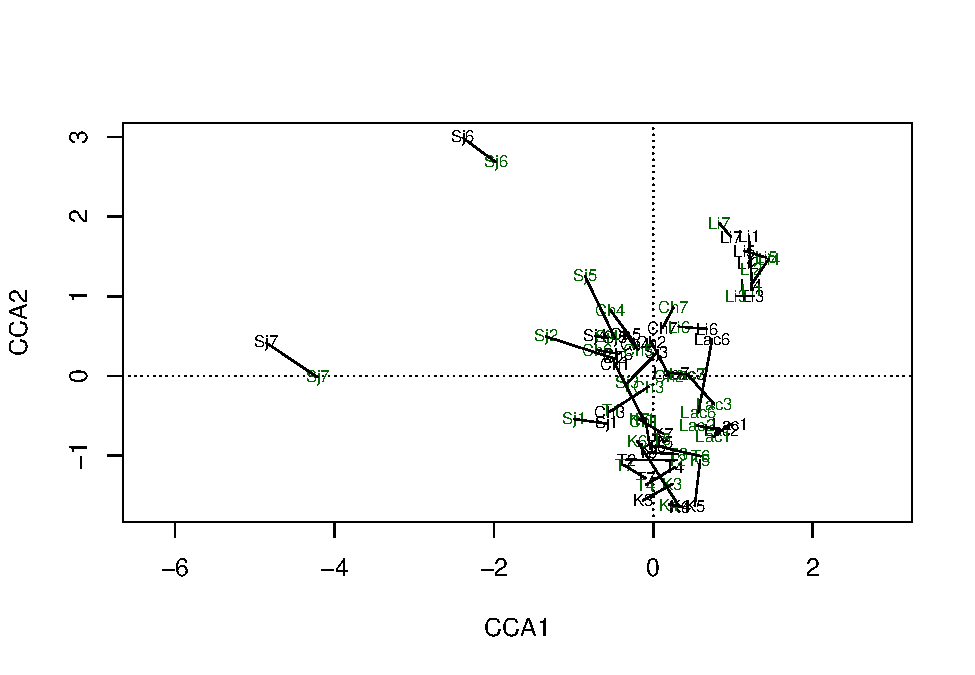
\includegraphics{05-multi2_files/figure-latex/unnamed-chunk-35-1.pdf}

\textbf{Figura 7:} Diferencias entre \emph{scores} de los sitios con LC y \emph{scores} de los sitios con WA en CCA.

\hypertarget{triplot-del-cca}{%
\subsubsection{Triplot del CCA}\label{triplot-del-cca}}

\begin{quote}
El código para producir triplots es similar al utilizado para RDA, excepto que las variables de respuesta (especies) están representadas por puntos y, por lo tanto, las flechas no están disponibles.
\end{quote}

\begin{Shaded}
\begin{Highlighting}[]
\CommentTok{\# saling=1: foco en la relación de distancias entre sitios}
\CommentTok{\# scores de sitios como promedios ponderados de la especie (WA)}
\FunctionTok{plot}\NormalTok{(cca\_DGGE,}\AttributeTok{scaling =} \DecValTok{1}\NormalTok{, }\AttributeTok{display =} \FunctionTok{c}\NormalTok{(}\StringTok{"sp"}\NormalTok{, }\StringTok{"lc"}\NormalTok{, }\StringTok{"cn"}\NormalTok{),}\AttributeTok{main =} \StringTok{"Triplot CCA DGGE {-}scaling 1"}\NormalTok{)}
\end{Highlighting}
\end{Shaded}

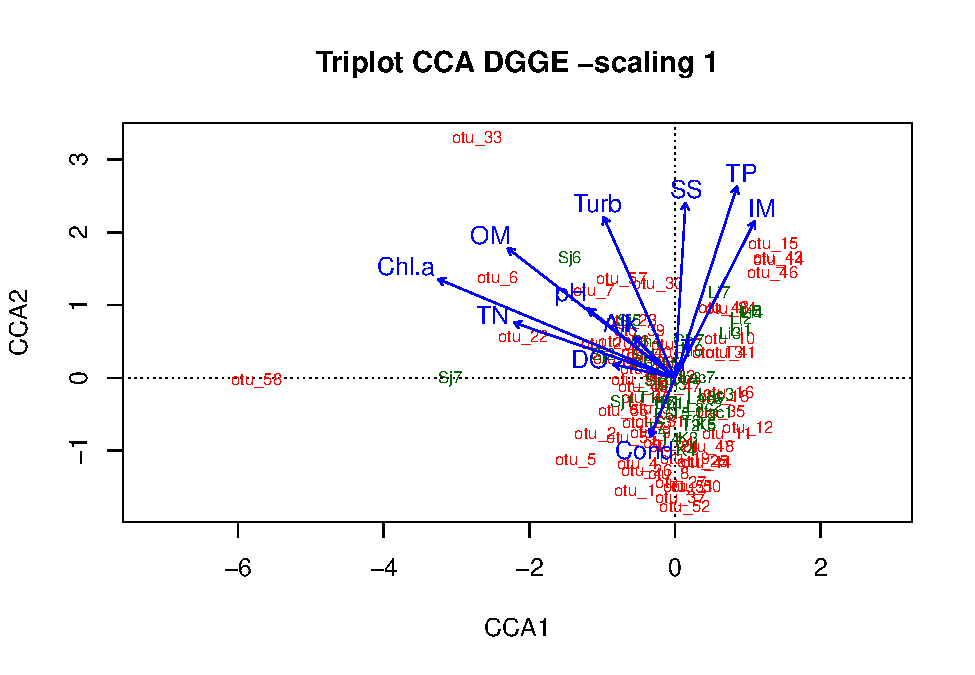
\includegraphics{05-multi2_files/figure-latex/unnamed-chunk-36-1.pdf}

\textbf{Figura 8:} Triplot del modelo completo de CCA con escalamiento 1.

\begin{Shaded}
\begin{Highlighting}[]
\CommentTok{\# Default scaling 2: foco en la relación de distancias entre otu\textquotesingle{}s, }
\CommentTok{\#scores de otu\textquotesingle{}s como promedio ponderado de los sitios (WA)}
\FunctionTok{plot}\NormalTok{(cca\_DGGE, }\AttributeTok{display =} \FunctionTok{c}\NormalTok{(}\StringTok{"sp"}\NormalTok{, }\StringTok{"lc"}\NormalTok{, }\StringTok{"cn"}\NormalTok{), }\AttributeTok{main =} \StringTok{"Triplot CCA DGGE {-} scaling 2"}\NormalTok{)}
\end{Highlighting}
\end{Shaded}

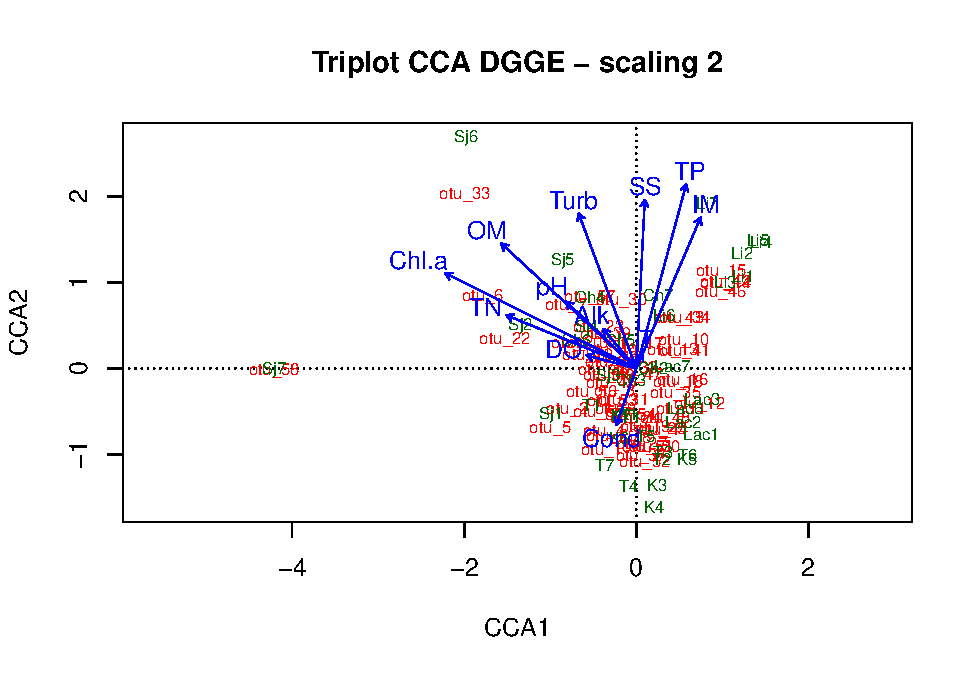
\includegraphics{05-multi2_files/figure-latex/unnamed-chunk-37-1.pdf}

\textbf{Figura 9:} Triplot del modelo completo de CCA con escalamiento 2.

\hypertarget{test-permutacionales-y-selecciuxf3n-de-variables}{%
\subsubsection{Test permutacionales y selección de variables}\label{test-permutacionales-y-selecciuxf3n-de-variables}}

\begin{quote}
La significación del modelo puede analizarse de la misma manera que para el RDA
\end{quote}

\begin{Shaded}
\begin{Highlighting}[]
\FunctionTok{anova}\NormalTok{(cca\_DGGE, }\AttributeTok{permutations =} \FunctionTok{how}\NormalTok{(}\AttributeTok{nperm =} \DecValTok{999}\NormalTok{))}\CommentTok{\#Modelo completo}
\end{Highlighting}
\end{Shaded}

\begin{verbatim}
## Permutation test for cca under reduced model
## Permutation: free
## Number of permutations: 999
## 
## Model: cca(formula = data_cca ~ Turb + DO + T + Cond + pH + Chl.a + TN + TP + SS + OM + IM + Alk, data = env.r)
##          Df ChiSquare      F Pr(>F)    
## Model    12    2.3497 1.5329  0.001 ***
## Residual 26    3.3212                  
## ---
## Signif. codes:  0 '***' 0.001 '**' 0.01 '*' 0.05 '.' 0.1 ' ' 1
\end{verbatim}

\begin{Shaded}
\begin{Highlighting}[]
\FunctionTok{anova}\NormalTok{(cca\_DGGE, }\AttributeTok{by =} \StringTok{"axis"}\NormalTok{, }\AttributeTok{permutations =} \FunctionTok{how}\NormalTok{(}\AttributeTok{nperm =} \DecValTok{999}\NormalTok{))}\CommentTok{\#Significación de los ejes}
\end{Highlighting}
\end{Shaded}

\begin{verbatim}
## Permutation test for cca under reduced model
## Forward tests for axes
## Permutation: free
## Number of permutations: 999
## 
## Model: cca(formula = data_cca ~ Turb + DO + T + Cond + pH + Chl.a + TN + TP + SS + OM + IM + Alk, data = env.r)
##          Df ChiSquare      F Pr(>F)   
## CCA1      1    0.5366 4.2011  0.007 **
## CCA2      1    0.3764 2.9464  0.011 * 
## CCA3      1    0.3502 2.7417  0.047 * 
## CCA4      1    0.2387 1.8686  0.722   
## CCA5      1    0.1981 1.5508  0.924   
## CCA6      1    0.1458 1.1417  1.000   
## CCA7      1    0.1356 1.0613  0.999   
## CCA8      1    0.1155 0.9038  1.000   
## CCA9      1    0.0908 0.7105  1.000   
## CCA10     1    0.0767 0.6006  1.000   
## CCA11     1    0.0517 0.4050  1.000   
## CCA12     1    0.0336 0.2629  1.000   
## Residual 26    3.3212                 
## ---
## Signif. codes:  0 '***' 0.001 '**' 0.01 '*' 0.05 '.' 0.1 ' ' 1
\end{verbatim}

\begin{Shaded}
\begin{Highlighting}[]
\CommentTok{\#Selección forward de variables}
\NormalTok{cca.step.forward }\OtherTok{\textless{}{-}}\FunctionTok{ordistep}\NormalTok{(}\FunctionTok{cca}\NormalTok{(data\_cca }\SpecialCharTok{\textasciitilde{}} \DecValTok{1}\NormalTok{, }\AttributeTok{data =}\NormalTok{ env.r), }\AttributeTok{scope =} \FunctionTok{formula}\NormalTok{(cca\_DGGE),}
\AttributeTok{direction =} \StringTok{"forward"}\NormalTok{, }\AttributeTok{permutations =} \FunctionTok{how}\NormalTok{(}\AttributeTok{nperm =} \DecValTok{199}\NormalTok{))}
\end{Highlighting}
\end{Shaded}

\begin{verbatim}
## 
## Start: data_cca ~ 1 
## 
##         Df    AIC      F Pr(>F)   
## + Chl.a  1 247.92 3.3236  0.005 **
## + OM     1 248.75 2.4791  0.005 **
## + TP     1 248.92 2.3023  0.005 **
## + TN     1 249.23 1.9917  0.005 **
## + Turb   1 249.31 1.9118  0.010 **
## + SS     1 249.43 1.7943  0.010 **
## + IM     1 249.34 1.8855  0.020 * 
## + pH     1 250.04 1.1904  0.285   
## + DO     1 250.33 0.9122  0.675   
## + Alk    1 250.54 0.7069  0.820   
## + Cond   1 250.57 0.6747  0.920   
## + T      1 250.57 0.6751  0.975   
## ---
## Signif. codes:  0 '***' 0.001 '**' 0.01 '*' 0.05 '.' 0.1 ' ' 1
## 
## Step: data_cca ~ Chl.a 
## 
##        Df    AIC      F Pr(>F)   
## + TP    1 247.31 2.4923  0.005 **
## + IM    1 247.82 1.9958  0.010 **
## + SS    1 247.96 1.8591  0.010 **
## + Turb  1 248.23 1.5960  0.045 * 
## + OM    1 248.57 1.2757  0.135   
## + TN    1 248.69 1.1618  0.195   
## + pH    1 248.96 0.8984  0.625   
## + DO    1 249.01 0.8576  0.635   
## + Cond  1 249.16 0.7171  0.905   
## + Alk   1 249.24 0.6383  0.935   
## + T     1 249.16 0.7173  0.940   
## ---
## Signif. codes:  0 '***' 0.001 '**' 0.01 '*' 0.05 '.' 0.1 ' ' 1
## 
## Step: data_cca ~ Chl.a + TP 
## 
##        Df    AIC      F Pr(>F)  
## + OM    1 247.69 1.4913  0.040 *
## + TN    1 247.95 1.2471  0.195  
## + Turb  1 248.03 1.1693  0.285  
## + SS    1 248.15 1.0624  0.395  
## + IM    1 248.28 0.9348  0.515  
## + pH    1 248.31 0.9083  0.595  
## + DO    1 248.34 0.8866  0.655  
## + T     1 248.49 0.7454  0.925  
## + Alk   1 248.59 0.6523  0.950  
## + Cond  1 248.64 0.6067  0.975  
## ---
## Signif. codes:  0 '***' 0.001 '**' 0.01 '*' 0.05 '.' 0.1 ' ' 1
## 
## Step: data_cca ~ Chl.a + TP + OM 
## 
##        Df    AIC      F Pr(>F)  
## + TN    1 248.10 1.4079  0.080 .
## + Turb  1 248.23 1.2906  0.085 .
## + IM    1 248.62 0.9454  0.465  
## + SS    1 248.62 0.9453  0.475  
## + DO    1 248.64 0.9231  0.540  
## + pH    1 248.64 0.9217  0.580  
## + T     1 248.62 0.9430  0.585  
## + Alk   1 248.69 0.8760  0.610  
## + Cond  1 248.68 0.8907  0.655  
## ---
## Signif. codes:  0 '***' 0.001 '**' 0.01 '*' 0.05 '.' 0.1 ' ' 1
\end{verbatim}

\hypertarget{elecciuxf3n-del-modelo}{%
\subsubsection{Elección del modelo}\label{elecciuxf3n-del-modelo}}

\begin{quote}
Con la expresión en base a la fórmula, observamos que tenemos control del modelo pero nos enfrentamos al dilema de elegir el ``mejor'' de los modelos.
Los modelos deben construirse con cuidado y, preferiblemente, utilizarse para probar
hipótesis específicas. En la construcción automática de modelos, generalmente necesitamos dos modelos extremos: el mínimo y el modelo completo. Con esos dos modelos, podemos implementar la función \textbf{step()} para seleccionar el mejor modelo. Esta función utiliza el criterio de información de Akaike (AIC) en la elección del modelo. El AIC se basa en la bondad de ajuste (alta inercia restringida/ variabilidad explicada), pero es penalizado por el número de parámetros estimados (rango restringido/ criterio de parsimonia). Los modelos alternativos se ordenan por AIC. En cada caso, ``+'' indica el efecto de agregar un término, y ``-'' el efecto de eliminar un término, mientras que el modelo que se evalua está marcado como ``''. Se debe tener mucho cuidado porque realmente no hay AIC para ordenaciones canónicas (¡aunque está calculada!), y siempre debemos inspeccionar la validez de elección del modelo.
\end{quote}

\begin{Shaded}
\begin{Highlighting}[]
\NormalTok{final\_cca }\OtherTok{\textless{}{-}} \FunctionTok{step}\NormalTok{(cca.step.forward, }\AttributeTok{scope=}\FunctionTok{formula}\NormalTok{(cca\_DGGE), }\AttributeTok{test=}\StringTok{"perm"}\NormalTok{)}
\end{Highlighting}
\end{Shaded}

\begin{verbatim}
## Start:  AIC=247.69
## data_cca ~ Chl.a + TP + OM
## 
##         Df    AIC      F Pr(>F)   
## - OM     1 247.31 1.4913  0.100 . 
## <none>     247.69                 
## - Chl.a  1 247.81 1.9596  0.020 * 
## + TN     1 248.10 1.4079  0.070 . 
## + Turb   1 248.23 1.2906  0.095 . 
## - TP     1 248.57 2.6824  0.005 **
## + IM     1 248.62 0.9454  0.435   
## + SS     1 248.62 0.9453  0.480   
## + T      1 248.62 0.9430  0.545   
## + DO     1 248.64 0.9231  0.620   
## + pH     1 248.64 0.9217  0.630   
## + Cond   1 248.68 0.8907  0.645   
## + Alk    1 248.69 0.8760  0.575   
## ---
## Signif. codes:  0 '***' 0.001 '**' 0.01 '*' 0.05 '.' 0.1 ' ' 1
## 
## Step:  AIC=247.31
## data_cca ~ Chl.a + TP
## 
##         Df    AIC      F Pr(>F)   
## <none>     247.31                 
## + OM     1 247.69 1.4913  0.050 * 
## - TP     1 247.92 2.4923  0.005 **
## + TN     1 247.95 1.2471  0.155   
## + Turb   1 248.03 1.1693  0.205   
## + SS     1 248.15 1.0624  0.365   
## + IM     1 248.28 0.9348  0.550   
## + pH     1 248.31 0.9083  0.620   
## + DO     1 248.34 0.8866  0.590   
## + T      1 248.49 0.7454  0.865   
## + Alk    1 248.59 0.6523  0.900   
## + Cond   1 248.64 0.6067  0.955   
## - Chl.a  1 248.92 3.4926  0.005 **
## ---
## Signif. codes:  0 '***' 0.001 '**' 0.01 '*' 0.05 '.' 0.1 ' ' 1
\end{verbatim}

\begin{quote}
Criterio AIC: cuanto más bajo el valor, mejor. Sin embargo, modelos con diferencias de AIC \textless{} 2 son igualmente válidos. En este caso, ambos modelos son válidos.
\end{quote}

\begin{Shaded}
\begin{Highlighting}[]
\CommentTok{\#Colinealidad de las variables}

\FunctionTok{vif.cca}\NormalTok{(cca\_DGGE)}
\end{Highlighting}
\end{Shaded}

\begin{verbatim}
##         Turb           DO            T         Cond           pH        Chl.a 
## 1.624592e+01 1.675050e+00 1.726303e+00 3.892686e+00 1.846872e+00 5.074104e+00 
##           TN           TP           SS           OM           IM          Alk 
## 2.052634e+00 5.642662e+00 4.859386e+08 5.514569e+07 3.413327e+08 3.391515e+00
\end{verbatim}

\begin{Shaded}
\begin{Highlighting}[]
\FunctionTok{vif.cca}\NormalTok{(cca.step.forward)}
\end{Highlighting}
\end{Shaded}

\begin{verbatim}
##    Chl.a       TP       OM 
## 2.340084 1.390174 2.865323
\end{verbatim}

\begin{Shaded}
\begin{Highlighting}[]
\FunctionTok{vif.cca}\NormalTok{(final\_cca)}
\end{Highlighting}
\end{Shaded}

\begin{verbatim}
##    Chl.a       TP 
## 1.013204 1.013204
\end{verbatim}

\emph{Notar que en el modelo completo Chl.a y TP presentan VIF \textgreater{} 5.}

\hypertarget{bibliografuxeda-citada-y-de-lectura-recomendada}{%
\subsection{Bibliografía citada y de lectura recomendada}\label{bibliografuxeda-citada-y-de-lectura-recomendada}}

Blanchet, F. G., P. Legendre, \& D. Borcard, 2008. Forward selection of explanatory variables. Ecology 89: 2623--2632.

Borcard, D., F. Gillet, \& P. Legendre, 2018. Numerical Ecology with R. Dairy Science \& Technology, CRC Taylor \& Francis Group. Springer International Publishing, Cham, \url{http://link.springer.com/10.1007/978-3-319-71404-2}.

Greenacre, M., 2008. Representación gráfica de distancias ji-cuadrado. La práctica del análisis de correspondencias 1--11.

Legendre, P., \& E. D. Gallagher, 2001. Ecologically meaningful transformations for ordination of species data. Oecologia 129: 271--280.

Lepš, J., \& P. Šmilauer, 2003. Multivariate Analysis of Ecological Data using CANOCO. .
Mcardle, B. H., M. J. Anderson, S. Ecology, \& N. Jan, 2014. Fitting Multivariate Models to Community Data: A Comment on Distance-Based Redundancy Analysis. Ecological Society of America 82: 290--297.

Llames M.E., P. A. del Giorgio, H. Zagarese, M. Ferraro \& I. Izaguirre, 2013. Alternative states drive the patterns in the bacterioplankton composition in shallow Pampean lakes (Argentina). Environmental Microbiology Reports 5(2): 310-321, \url{https://doi.org/10.1111/1758-2229.12020}.

Oksanen, J., 2008. Vegan: an introduction to ordination. R- packace Vegan 1: 1--10, \url{http://doi.acm.org/10.1145/2037556.2037605\%5Cnftp://ftp3.ie.freebsd.org/pub/cran.r-project.org/web/packages/vegan/vignettes/intro-vegan.pdf}.

Oksanen, J., 2009. Design decisions and implementation details in vegan. R- packace Vegan 2: 1--11.

Oksanen, J., 2012. Constrained ordination: tutorial with R and vegan. R- packace Vegan 1--10.

Peres-Neto, P. R., P. Legendre, S. Dray, \& D. Borcard, 2006. VARIATION PARTITIONING OF SPECIES DATA MATRICES: ESTIMATION AND COMPARISON OF FRACTIONS PEDRO. 87: 2614--2625.

Quiroga, M. V., G. Mataloni, B. M. S. Wanderley, A. M. Amado \& F. Unrein, 2017. Bacterioplankton morphotypes structure and cytometric fingerprint rely on environmental conditions in a sub-Antarctic peatland. Hydrobiologia 787: 255-268, \url{https://doi.org/10.1007/s10750-016-2969-2}.

Zuur, A. F., E. N. Ieno, \& G. M. Smith, 2007. Analysing Ecological Data. Springer New York, New York, NY, \url{http://link.springer.com/10.1007/978-0-387-45972-1}.

\hypertarget{metrix}{%
\chapter{\texorpdfstring{Paquete \emph{metrix}}{Paquete metrix}}\label{metrix}}

\textbf{Julieta Capeletti}\footnote{\href{mailto:julieta.capeletti@hotmail.com}{\nolinkurl{julieta.capeletti@hotmail.com}}}

Instituto Nacional de Limnología (INALI, UNL-CONICET), Laboratorio de Bentos

\textbf{Juan Manuel Cabrera}\footnote{\href{mailto:juan.cabrera@uner.edu.ar}{\nolinkurl{juan.cabrera@uner.edu.ar}}}

Instituto de Investigación y Desarrollo en Bioingeniería y Bioinformática (IBB, UNER-CONICET)

\hypertarget{que-es-metrix}{%
\section{¿Que es Metrix?}\label{que-es-metrix}}

\emph{metrix} es un paquete de R de código abierto diseñado específicamente para evaluar la calidad del agua utilizando datos de densidad de macroinvertebrados \citep{cabrera2023}.
Este paquete nos permite calcular una extensa cantidad de métricas e índices bióticos que evalúan la calidad del ambiente de manera rápida y sencilla.
Admite una resolución taxonómica heterogénea que permite cálculos en varios niveles taxonómicos y es capaz de leer hojas de cálculo biológicas a partir de grandes volúmenes de datos.
Este paquete facilita la manipulación de datos, simplificando el proceso mediante el uso de hojas de cálculo predefinidas en formato .csv.
Esto reduce la necesidad de software o paquetes adicionales, haciéndolo accesible y fácil de usar, incluso para usuarios sin conocimientos de programación.
Las futuras versiones del paquete pueden incluir otros índices métricos y bióticos, mejorando aún más sus capacidades.
Además, se puede desarrollar una interfaz fácil de usar para mejorar la usabilidad de la herramienta para usuarios no científicos, como las agencias gubernamentales responsables de evaluar el impacto ambiental de las actividades relacionadas con los seres humanos.

\hypertarget{conjunto-de-datos-de-ejemplo}{%
\section{Conjunto de datos de ejemplo}\label{conjunto-de-datos-de-ejemplo}}

Antes de comenzar a probar \emph{metrix}, vamos a descargar el conjunto de datos perteneciente a muestreos en la cuenca Cañada Carrizales localizada en la ecorregión Pampeana de Argentina (32°26'23.53 ``S, 61°18'10.69''W), perteneciente al trabajo \emph{Métricas basadas en macroinvertebrados como monitores de ambientes con uso de suelo agrícola: estudio preliminar en una cuenca pampeana} \citep{capeletti2019}.
El conjunto de datos está disponible en la carpeta \emph{data} del repositorio de GitHub de \emph{metrix} \url{https://github.com/Dvelop-R/metrix}.

\hypertarget{instalar-metrix}{%
\section{\texorpdfstring{Instalar \emph{metrix}}{Instalar metrix}}\label{instalar-metrix}}

\emph{metrix} se encuentra disponible en el repositorio CRAN.
Primeramente se debe descargar e instalar utilizando el código \texttt{install.packages("metrix")}.
Seguidamente se debe cargar el paquete en el entorno de trabajo:

\begin{Shaded}
\begin{Highlighting}[]
\FunctionTok{library}\NormalTok{(metrix)}
\end{Highlighting}
\end{Shaded}

\hypertarget{que-tipos-de-datos-analiza-metrix}{%
\section{\texorpdfstring{¿Que tipos de datos analiza \emph{metrix}?}{¿Que tipos de datos analiza metrix?}}\label{que-tipos-de-datos-analiza-metrix}}

\emph{metrix} utiliza un formato específico de tabla de datos.
La misma consiste en 8 columnas que representen la clasificación científica y funcional de los taxones:

\begin{itemize}
\item
  Las primeras 7 columnas corresponden a \emph{Clase}, \emph{Orden}, \emph{Familia}, \emph{Subfamilia}, \emph{Tribu}, \emph{Género} y \emph{Especie}.
\item
  La columna 8 indica el \emph{grupo funcional} (FG) de los taxones, que puede ser \emph{recolectores filtradores} (GF), \emph{colectores recolectores} (GC), \emph{depredadores} (P), \emph{raspadores} (SCR), o \emph{trituradores} (SHR).
\item
  Después de estas columnas, se debe incluir los \emph{datos de densidad (individuos/m2)} de los macroinvertebrados para cada muestra de sitio.
\end{itemize}

Durante el proceso de carga de datos es muy común que se cometan errores de tipeo que pueden llevar a que no se pueda identificar de manera correcta a los taxa incluidos en el conjunto de datos.
\emph{metrix} posee un sistema de autocorreción que puede asisitir al usuario en la identificación de estas fallas en la carga de datos.
Para ello utiliza una base de datos de nombres cientificos utilizados en la descripción de los taxones que son tenidos en cuenta a la hora de calcular las métricas e índices bióticos calculados por el paquete.
Este sistema de autocorrección informa al usuario sobre posibles errores de carga y, si el usuario lo indica, puede corregirlo de manera automática (con un criterio de similitud de palabra).

\hypertarget{cargar-datos-de-densidad-de-macroinvertebrados-usando-metrix}{%
\section{\texorpdfstring{Cargar datos de densidad de macroinvertebrados usando \emph{metrix}}{Cargar datos de densidad de macroinvertebrados usando metrix}}\label{cargar-datos-de-densidad-de-macroinvertebrados-usando-metrix}}

Para cargar los datos en el entorno de trabajo de R utilizamos la función \texttt{read\_data()}.
Esta función recibe 3 parámatros:

\begin{itemize}
\item
  \emph{file\_name}: dirección/nombre del archivo .csv que contiene los datos de densidad de macroinvertebrados.
\item
  \emph{correct}: valor lógico que indica si se va a utilizar el sistema de autocorrección de datos.
\item
  \emph{verbose}: valor lógico que indica si se debe mostrar mensajes descriptivos del proceso de carga.
\end{itemize}

\begin{Shaded}
\begin{Highlighting}[]
\CommentTok{\#IMPORTANTE: revisar la dirección del archivo ecological\_data.csv. En este ejemplo estaría dentro del directorio de trabajo por lo que no es necesario indicar la ruta completa al archivo}
\NormalTok{datos\_cargados}\OtherTok{\textless{}{-}}\FunctionTok{read\_data}\NormalTok{(}\AttributeTok{file\_name =} \StringTok{"ecological\_data.csv"}\NormalTok{, }\AttributeTok{correct =} \ConstantTok{TRUE}\NormalTok{, }\AttributeTok{verbose =} \ConstantTok{FALSE}\NormalTok{)}
\end{Highlighting}
\end{Shaded}

\begin{verbatim}
## The word ampullaridae was not found in internal Family word database. Please check that entry.
\end{verbatim}

\begin{verbatim}
## The autocorrect system replace the word ampullaridae for Ampullariidae.
\end{verbatim}

En este ejemplo, los datos ecológicos utilizados contienen un error en la columna de \emph{Familia}.
El sistema de autocorrección notificará al usuario sobre este error y, si el parámetro \texttt{correct} está seteado con el valor \texttt{TRUE}, reemplazará la palabra presuntamente erronea por otra similar hallada en la base de datos interna.

\hypertarget{que-pasa-si-quiero-crear-mi-propio-conjunto-de-datos}{%
\subsection{¿QUE PASA SI QUIERO CREAR MI PROPIO CONJUNTO DE DATOS?}\label{que-pasa-si-quiero-crear-mi-propio-conjunto-de-datos}}

\emph{metrix} contiene una función que genera un archivo .CSV con una tabla cuyas columnas están debidamente etiquetadas para que pueda ser utilizada por el paquete.
Para generar este archivo en el espacio de trabajo, se debe correr el siguiente código:

\begin{Shaded}
\begin{Highlighting}[]
\FunctionTok{metrix\_table\_template}\NormalTok{()}
\end{Highlighting}
\end{Shaded}

\begin{verbatim}
##     Class   Order       Family    Subfamily       Tribe          Genus Species
## 1 Insecta Diptera Chironomidae Chironominae Tanytarsini Paratanytarsus        
##   FG Sample1 Sample2
## 1 GC       1       0
\end{verbatim}

Una vez generado el archivo se puede editar el mismo utilizando un bloc de notas o una editor de hojas de cálculo.
Luego se puede cargar al entorno de trabajo de igual manera que en el paso anterior.

\hypertarget{cuxe1lculo-de-metricas-individuales-y-ecoluxf3gicas}{%
\section{Cálculo de metricas individuales y ecológicas}\label{cuxe1lculo-de-metricas-individuales-y-ecoluxf3gicas}}

Para evaluar la calidad biológica del agua, es necesario examinar valores específicos que midan características clave de la comunidad de macroinvertebrados, las cuales son indicativas de su respuesta a degradaciones ambientales.
\emph{metrix} incluye una amplia gama de cálculos tanto para métricas individuales como ecológicas: * \emph{Métricas individuales}: abarcan la riqueza, que indica la diversidad del conjunto de macroinvertebrados; las métricas de composición, que calculan la abundancia relativa de taxones específicos dentro de la comunidad en términos de porcentajes; y las métricas de densidad, que sirven como medidas universales utilizadas en todo tipo de estudios biológicos.
* \emph{Métricas ecológicas}: incluyen métricas tróficas (como la riqueza de depredadores, la riqueza de colectores recolectores, la densidad de trituradores y la densidad de raspadores), que actúan como indicadores de procesos complejos como las interacciones tróficas, la producción y la disponibilidad de fuentes de alimento.
Además, se incluyen medidas de tolerancia para indicar la sensibilidad de la comunidad y especies individuales a varios tipos de perturbaciones.

En este ejemplo vamos a calcular metricas de riqueza de nuestro conjunto de datos previamente cargados.
Para ello vamos a utilizar la función \texttt{rich\_metrics()}, la cual recibe 4 parámetros:

\begin{itemize}
\tightlist
\item
  \emph{dataset}: conjunto de datos cargados con la función \texttt{read\_data()}.
\item
  \emph{store}: valor lógico que indica si el resultado debe ser almacenado en un archivo.
\item
  \emph{dec\_c}: caracter utilizado como separador de decimales.
\item
  \emph{verbose}: valor lógico que indica si se debe mostrar mensajes descriptivos del calcúlo realizado.
\end{itemize}

\begin{Shaded}
\begin{Highlighting}[]
\CommentTok{\#Calculo de riqueza}
\FunctionTok{rich\_metrics}\NormalTok{(}\AttributeTok{dataset =}\NormalTok{ datos\_cargados, }\AttributeTok{store =} \ConstantTok{FALSE}\NormalTok{, }\AttributeTok{dec\_c =} \StringTok{"."}\NormalTok{, }\AttributeTok{verbose =} \ConstantTok{TRUE}\NormalTok{)}
\end{Highlighting}
\end{Shaded}

\begin{verbatim}
## Checking table format for Richness measures calculation...
\end{verbatim}

\begin{verbatim}
##                    P1 P2 P3 P4 P5 P6 P7 P8 P9 P10
## n_taxa              4  7  7  7  6  6  4  6  8   4
## n_fam               4  3  6  5  6  6  4  6  7   3
## n_gen               4  6  4  5  5  6  4  6  6   4
## n_insec_fam         2  1  4  2  3  2  2  2  4   1
## n_non_insec_order   2  2  2  2  3  3  2  3  3   2
## n_dip_fam           1  1  3  2  2  1  1  1  3   1
## n_dip_gen           1  4  1  1  1  1  1  1  2   1
## n_dip_chir_gen      1  4  1  1  1  1  1  1  2   1
## n_chir_tax          1  4  1  1  1  1  1  1  2   1
## n_tany_tax          0  0  0  0  0  0  0  0  0   0
## n_stemp_tax         0  0  0  0  0  0  0  0  0   0
## n_non_chir_dip_tax  0  0  2  1  1  0  0  0  2   0
## n_mol_tax           1  1  1  2  1  2  1  2  1   1
## n_gastr_tax         1  1  1  2  1  2  1  2  1   1
## n_biv_tax           0  0  0  0  0  0  0  0  0   0
## n_crus_tax          0  0  0  0  1  1  1  1  1   0
## n_crusmol           1  1  1  2  2  3  2  3  2   1
## n_oligo_tax         1  2  2  3  1  1  0  1  1   2
## n_ephetrich         0  0  0  0  0  0  0  0  1   0
\end{verbatim}

Los sitios P1, P7 y P10 son los que menor riqueza presentan, a diferencia de los demás sitios.
En estos sitios la riqueza se da principalmente por la presencia de los órdenes de Diptera, Mollusca, Crustacea y Oligochaeta.

También podemos calcular métricas de tolerancia utilizando la función \texttt{tol\_metrics()}.
Esta función recibe 4 parámetros:

\begin{itemize}
\tightlist
\item
  \emph{dataset}: conjunto de datos cargados con la función \texttt{read\_data()}.
\item
  \emph{store}: valor lógico que indica si el resultado debe ser almacenado en un archivo.
\item
  \emph{dec\_c}: caracter utilizado como separador de decimales.
\item
  \emph{verbose}:valor lógico que indica si se debe mostrar mensajes descriptivos del calcúlo realizado.
\end{itemize}

\begin{Shaded}
\begin{Highlighting}[]
\CommentTok{\#Calculo de metricas de tolerancia}
\FunctionTok{tol\_metrics}\NormalTok{(}\AttributeTok{dataset =}\NormalTok{ datos\_cargados, }\AttributeTok{store =} \ConstantTok{FALSE}\NormalTok{, }\AttributeTok{dec\_c =} \StringTok{"."}\NormalTok{, }\AttributeTok{verbose =} \ConstantTok{TRUE}\NormalTok{)}
\end{Highlighting}
\end{Shaded}

\begin{verbatim}
## Checking table format for Tolerance measures calculation...
\end{verbatim}

\begin{verbatim}
##                 P1     P2     P3     P4     P5     P6    P7     P8    P9    P10
## r_oligochir 0.0066 0.0054 0.0278 0.6667 0.0357 0.0085 0.000 0.0313 0.100 3.3333
## r_oligoset  0.0000 0.0000 0.0000 0.0000 0.0000 0.0000 0.000 0.0000 0.000 0.0000
## r_tanychir  0.0000 0.0000 0.0000 0.0000 0.0000 0.0000 0.000 0.0000 0.000 0.0000
## den_t_lhoff 0.0000 0.0000 0.0000 0.0000 0.0000 0.0000 0.000 0.0000 0.000 0.0000
## den_t_bothr 0.0000 0.0000 0.0000 0.0000 0.0000 0.0000 0.000 0.0000 0.000 0.0000
## den_t_tubi  0.0000 0.0000 0.0000 0.0000 0.0000 0.0000 0.000 0.0000 0.000 0.0000
## den_t_dero  0.0000 0.0000 0.0000 0.0000 0.0000 0.0000 0.000 0.0000 0.000 0.0000
## den_t_prist 0.0000 0.0000 0.0000 0.0000 0.0000 0.0000 0.000 0.0000 0.000 0.0000
## den_t_chiro 0.0000 0.0000 0.0000 0.0000 0.0000 0.0000 0.000 0.0000 0.000 0.0000
## den_t_hele  0.5740 0.5740 0.5740 0.5740 0.5740 0.5740 0.574 0.5740 0.574 0.5740
\end{verbatim}

La relación de la densidad de Oligochaeta/Chironomidae nos permitiría diferenciar los sitios de acuerdo a su gradiente de impacto.
Esta métrica disminuye a medida que aumenta ladegradación, por lo tanto los sitios con los valores más altos serían los más contaminados a diferencia de los sitios con los valores más bajo los cuales presentarían condiciones de referencia.
La métrica Heleobia/DT presenta el mismo valor en todos los sitios por lo tanto no nos estaría diferenciando los sitios de acuerdo a su gradiente de impacto antrópico.

\hypertarget{cuxe1lculo-de-indices-biuxf3ticos}{%
\section{Cálculo de indices bióticos}\label{cuxe1lculo-de-indices-biuxf3ticos}}

Los índices bióticos comprenden una combinación de dos o tres métricas individuales o ecológicas, que se condensan en un único valor que resume las características biológicas de todos los organismos presentes.
Para los índices cualitativos, estas métricas incluyen la riqueza de taxones y la sensibilidad a la contaminación.
Para los índices cuantitativos se incorpora la abundancia (absoluta o relativa).
\emph{metrix} incluye cálculos para los siguientes índices bióticos:

\begin{itemize}
\item
  \emph{BMWP} (Biological Monitoring Working Party, \citep{armitage1983}), \emph{ASPT} (Average Score per Taxon, \citep{armitage1983}) y sus adaptaciones: \emph{BMWP'} \citep{alba1988} y \emph{BMWP'\,'} \citep{loyola2000}.
  Estos índices utilizan la presencia y abundancia de ciertas familias de macroinvertebrados.
  A cada familia se le asigna un valor de puntuación basado en su tolerancia a la contaminación (de 0 a 10).
  Las familias más sensibles a la contaminación reciben puntuaciones más altas, mientras que las familias más tolerantes reciben puntuaciones más bajas.
  Las puntuaciones de todas las familias de organismos presentes en una muestra de agua se suman para obtener el valor total del índice y determinar la calidad del agua.
\item
  \emph{IMRP} (Índice de Macroinvertebrados en Ríos Pampeanos, \citep{rodrigues1999}).
  Este índice se basa en la presencia y abundancia de ciertos órdenes y familias de macroinvertebrados para determinar la calidad del agua.
  Al igual que los índices BMWP, a cada grupo se le asigna un valor de puntuación basado en su tolerancia a la contaminación (en este caso, de 0 a 1), siendo el valor final del índice la suma de todos los órdenes o familias presentes en la muestra.
\item
  \emph{ICBrio} (Índice das Comunidades Benticas em Ríos, \citep{kuhlmann2012}).
  Este índice utiliza los valores de densidad total de la muestra y se basa en la tolerancia de los organismos a la contaminación y su respuesta a las perturbaciones ambientales.
  El índice asigna valores de puntuación a diferentes grupos taxonómicos (a nivel de orden, familia y género) de macroinvertebrados presentes en las muestras.
  Estas puntuaciones se suman luego para obtener un valor total del índice y determinar la calidad del agua.
\end{itemize}

En este ejemplo vamos a calcular los indices \emph{BMWP} e \emph{ICBrio}.
Para ello vamos a utilizar las funciones \texttt{bmwp\_ind()} e \texttt{icbrio\_ind()}.
Ambas funciones reciben 4 parámetros:

\begin{itemize}
\tightlist
\item
  \emph{dataset}: conjunto de datos cargados con la función \texttt{read\_data()}.
\item
  \emph{store}: valor lógico que indica si el resultado debe ser almacenado en un archivo.
\item
  \emph{dec\_c}: caracter utilizado como separador de decimales.
\item
  \emph{verbose}:valor lógico que indica si se debe mostrar mensajes descriptivos del calcúlo realizado.
\end{itemize}

\begin{Shaded}
\begin{Highlighting}[]
\CommentTok{\#Calculo de BMWP}
\FunctionTok{bmwp\_ind}\NormalTok{(}\AttributeTok{dataset =}\NormalTok{ datos\_cargados, }\AttributeTok{store =} \ConstantTok{FALSE}\NormalTok{, }\AttributeTok{dec\_c =} \StringTok{"."}\NormalTok{, }\AttributeTok{verbose =} \ConstantTok{TRUE}\NormalTok{)}
\end{Highlighting}
\end{Shaded}

\begin{verbatim}
## Checking table format for BMWP and ASPT index calculation...
\end{verbatim}

\begin{verbatim}
## $Ibmwp_n
##          P1  P2 P3  P4 P5 P6 P7 P8  P9 P10
## ind_bmwp  9 3.0  9 3.0  9 12  8 12 3.0 3.0
## ind_aspt  3 1.5  3 1.5  3  3  4  3 1.5 1.5
## 
## $Ibmwp_c
##                                P1                 P2                 P3
## ind_bmwp_class Class VII Very Bad Class VII Very Bad Class VII Very Bad
## ind_aspt_class       Class VI Bad Class VII Very Bad       Class VI Bad
##                                P4                 P5                 P6
## ind_bmwp_class Class VII Very Bad Class VII Very Bad Class VII Very Bad
## ind_aspt_class Class VII Very Bad       Class VI Bad       Class VI Bad
##                                P7                 P8                 P9
## ind_bmwp_class Class VII Very Bad Class VII Very Bad Class VII Very Bad
## ind_aspt_class   Class V Moderate       Class VI Bad Class VII Very Bad
##                               P10
## ind_bmwp_class Class VII Very Bad
## ind_aspt_class Class VII Very Bad
\end{verbatim}

Los valores de BMWP y ASPT nos indican condiciones de mala calidad en los 10 puntos de muestreo.

\begin{Shaded}
\begin{Highlighting}[]
\CommentTok{\#Calculo de ICBrio}
\FunctionTok{icbrio\_ind}\NormalTok{(}\AttributeTok{dataset =}\NormalTok{ datos\_cargados, }\AttributeTok{store =} \ConstantTok{FALSE}\NormalTok{, }\AttributeTok{dec\_c =} \StringTok{"."}\NormalTok{, }\AttributeTok{verbose =} \ConstantTok{TRUE}\NormalTok{)}
\end{Highlighting}
\end{Shaded}

\begin{verbatim}
## Checking table format for ICbrio index calculation...
\end{verbatim}

\begin{verbatim}
## $Icbrio_n
##                  P1 P2 P3 P4       P5 P6 P7       P8   P9      P10
## ind_icbrio 4.333333  4  4  4 3.666667  4  6 3.666667 2.75 4.333333
## 
## $Icbrio_c
##                   P1  P2  P3  P4  P5  P6  P7  P8      P9 P10
## ind_icbrio_class Bad Bad Bad Bad Bad Bad Bad Bad Regular Bad
\end{verbatim}

De igual manera el indice ICBRio nos indica que 9 sitios presentan una condición biológica mala, mientras que 1 sitio (P9) presenta regulares condiciones.

\hypertarget{futuro-del-paquete}{%
\section{FUTURO DEL PAQUETE}\label{futuro-del-paquete}}

Las futuras versiones del paquete podrían incluir otras métricas e índices bióticos, mejorando aún más sus capacidades.
Además, puede que se desarrolle una interfaz amigable para el usuario, mejorando la usabilidad de la herramienta para usuarios no científicos, como agencias gubernamentales encargadas de evaluar el impacto ambiental de actividades relacionadas con el ser humano.

\hypertarget{agradecimientos-1}{%
\section{AGRADECIMIENTOS}\label{agradecimientos-1}}

Agradecemos a la Dra.
Florencia Zilli, Dra.
Mercedes Marchese y Dr.~Joaquien Cochero por su ayuda y apoyo en la creación de esta herramienta.

\hypertarget{diathor}{%
\chapter{\texorpdfstring{Paquetes \emph{DiaThor} y \emph{optimos.prime}}{Paquetes DiaThor y optimos.prime}}\label{diathor}}

\textbf{Joaquín Cochero}\footnote{\href{mailto:jcochero@ilpla.edu.ar}{\nolinkurl{jcochero@ilpla.edu.ar}}}

\hypertarget{paquete-diathor}{%
\section{\texorpdfstring{Paquete \emph{DiaThor}}{Paquete DiaThor}}\label{paquete-diathor}}

\emph{Autores: María Mercedes Nicolosi Gelis}\footnote{\href{mailto:mercedesnicolosi@ilpla.edu.ar}{\nolinkurl{mercedesnicolosi@ilpla.edu.ar}}}\emph{, María Belén Sathicq}\footnote{\href{mailto:mbelen@ilpla.edu.ar}{\nolinkurl{mbelen@ilpla.edu.ar}}}\emph{, Joaquín Cochero}

\hypertarget{quuxe9-hace}{%
\subsection{¿Qué hace?}\label{quuxe9-hace}}

El paquete calcula múltiples \textbf{índices bióticos y ecológicos basados en diatomeas} a partir de datos de abundancia en muestras ambientales.

\hypertarget{cuxf3mo-funciona}{%
\subsection{¿Cómo funciona?}\label{cuxf3mo-funciona}}

El paquete obtiene las \textbf{preferencias ecológicas} de los taxones de diatomeas vinculandolos por nombre a las bases de datos de cada índice biótico y ecológico. Realiza una búsqueda exacta y luego heurística del nombre del taxón comparandola contra distintas \protect\hyperlink{fuentes-de-informaciuxf3n-ecoluxf3gica-de-las-especies}{Fuentes de información ecológica de las especies}.

Una vez que encuentra la especie en cada alguna de las bases de datos de los distintos índices, realiza los cálculos de los índices en base a su abundancia en las muestras, y devuelve una tabla con los valores de cada índice por muestra ingresada.

\hypertarget{manos-a-la-obra-1}{%
\subsection{¡Manos a la obra!}\label{manos-a-la-obra-1}}

Vamos a utilizar el set de datos del trabajo \emph{``Exploring the use of nuclear alterations, motility and ecological guilds in epipelic diatoms as biomonitoring tools for water quality improvement in urban impacted lowland streams'',} de Nicolosi Gelis et al.~(2020) \citep{nicolosigelis2020} publicado en Ecological Indicators y disponible en el \href{https://ri.conicet.gov.ar/handle/11336/128216}{Repositorio Institucional CONICET Digital}.

\hypertarget{descargar-los-datos}{%
\subsubsection{\texorpdfstring{\textbf{Descargar los datos}}{Descargar los datos}}\label{descargar-los-datos}}

Descargar los datos de ejemplo desde el repositorio del curso y guardar el archivo en el Directorio de Trabajo del Proyecto que creamos para esta Unidad (ver cómo hacerlo en la Unidad \ref{intro}).

Datos de ejemplo aquí: \url{https://github.com/Limno-con-R/CILCAL2023/blob/main/datasets/sampleData_diaThor.csv}

\hypertarget{instalar-el-paquete}{%
\subsubsection{Instalar el paquete}\label{instalar-el-paquete}}

Instalaremos el paquete \texttt{diaThor}\citep{nicolosigelis2022} como se indica en la Unidad \ref{intro} y los cargaremos a nuestro espacio de trabajo actual:

\begin{Shaded}
\begin{Highlighting}[]
\FunctionTok{library}\NormalTok{(diathor)}
\end{Highlighting}
\end{Shaded}

\hypertarget{cargar-y-previsualizar-nuestro-archivo-de-datos}{%
\subsubsection{Cargar y previsualizar nuestro archivo de datos}\label{cargar-y-previsualizar-nuestro-archivo-de-datos}}

Cargaremos nuestro archivo de ejemplo (\emph{sampleData\_diaThor.csv}) a un dataframe llamado ``base'':

\begin{Shaded}
\begin{Highlighting}[]
\NormalTok{base }\OtherTok{\textless{}{-}} \FunctionTok{read.csv}\NormalTok{(}\StringTok{"sampleData\_diaThor.csv"}\NormalTok{) }\CommentTok{\#Corroborar que el nombre del archivo coincida con el que vamos a utilizar, y que se encuentre en la carpeta de nuestro proyecto}
\end{Highlighting}
\end{Shaded}

Veamos brevemente cómo está organizada la información de nuestras especies:

\begin{Shaded}
\begin{Highlighting}[]
\FunctionTok{str}\NormalTok{(base)}
\end{Highlighting}
\end{Shaded}

\texttt{base} es un objeto \texttt{data.frame} con 164 \texttt{obs.} o filas (especies) y 110 \texttt{variables} o columnas (muestras).

Nuestra planilla de datos además contiene una \textbf{columna obligatoria} llamada ``\textbf{\emph{species}}'', la primera, adonde debremos ingresar los nombres de las especies lo mejor que podamos, sin datos sobre autorías de las mismas.

\emph{Ejemplo de cómo llamar a las especies:}

\emph{Hippodonta capitata} ------------\textgreater{} (ASI SI! ✔️)

\emph{Hippodonta capitata} (Ehrenb.) Lange-Bert., Metzeltin and Witkowski 1996 ------------\textgreater{} (ASI NO! 🚫)

Veamos las primeras filas y las primeras columnas:

\begin{Shaded}
\begin{Highlighting}[]
\FunctionTok{head}\NormalTok{(base[}\DecValTok{1}\SpecialCharTok{:}\DecValTok{10}\NormalTok{, }\DecValTok{1}\SpecialCharTok{:}\DecValTok{5}\NormalTok{])}
\end{Highlighting}
\end{Shaded}

\begin{verbatim}
##   X                        species S1_LI1_DAY0 S1_LI2_DAY0 S1_LI3_DAY0
## 1 1   Achnanthidium minutissimum             0           0           0
## 2 2 Achnanthes exigua var. exigua            0           0           0
## 3 3               Amphora libyca             0           0           0
## 4 4     Anomoeoneis sphaerophora             0           0           0
## 5 5            Craticula ambigua             0           0           1
## 6 6            Caloneis bacillum             0           0           0
\end{verbatim}

Cada columna representa \textbf{a una muestra}.\\
Debe contener un nombre de muestra (\emph{por ejemplo, se llaman S1\_LI1\_DAY0, S1\_LI2\_DAY0, etc.}).

\textbf{NOTA}: Los valores en las celdas pueden ser valores de densidad absoluta (como es en este ejemplo) o abundancia relativa. Por defecto, \emph{diaThor} asume que las densidades son absolutas; si queremos cambiar esta opción, debemos pasar el parámetro \texttt{isRelAb=FALSE} a \texttt{isRelAb=TRUE} cuando usamos las funciones.

\hypertarget{a-la-magia}{%
\subsubsection{\texorpdfstring{\textbf{¡A la magia!}}{¡A la magia!}}\label{a-la-magia}}

Vamos a ejecutar la función \texttt{diaThorAll()} , que se encargará de realizar \textbf{todos los análisis que puede realizar el paquete}, una atrás de otra. Y dispondremos de los resultados en un único objeto de tipo \texttt{data.frame}, que aquí lo llamaremos \texttt{resultados}.

Más adelante veremos que podemos solicitar cosas específicas si sólo necesitamos un tipo de resultado, para ahorrar tiempo y reducir la cantidad de salidas.

\begin{Shaded}
\begin{Highlighting}[]
\NormalTok{resultados }\OtherTok{\textless{}{-}} \FunctionTok{diaThorAll}\NormalTok{(base)}
\end{Highlighting}
\end{Shaded}

El paquete nos irá mostrando información en la consola de RStudio, y nos solicitará que le indiquemos una carpeta adonde guardar todas las posibles salidas que vaya generando. Exploraremos estas salidas luego para tratar de mejorar los resultados.

\texttt{{[}1{]}\ "Select\ Results\ folder"}

Seleccionemos un directorio (preferentemente vacío!) para guardar las salidas, y el paquete continuará reconociendo las especies, y buscando información ecológica sobre ellas para calcular los distintos índices bióticos.

\hypertarget{los-resultados}{%
\subsubsection{Los resultados}\label{los-resultados}}

Si todo ha salido bien, \emph{diaThor} debería haber calculado todos los índices posibles.

Cuando los índices bióticos se publican, no necesariamente se le asigna un valor ecológico a todas las especies de diatomeas (\emph{hay unas 200.000 especies}!). Hay índices que sólo contemplan menos de 300 especies (ejemplos: \emph{IDP}, \emph{SPEAR} o los de Lobo et al.), y otros incluyen más de 6000 (ejemplo: \emph{IPS}).

\textbf{En la consola veremos que porcentaje del listado de especies que ingresamos fue efectivamente utilizado para calcular cada índice.} Por ejemplo -\textgreater{} \emph{``Taxa recognized to be used in DISP index: 22.6 \%''}, nos indica que de nuestras 164 especies, sólo utilizó 22.6\% para calcular el índice DISP, mientras que dejó afuera el 77.4\%. Es importante entonces delimitar qué índices fueron calculados sobre una base sólida de nuestros datos al momento de interpretar los resultados.

El final de la secuencia de cálculo en la consola está delimitado por la exportación de gráficos (\emph{{[}1{]} ``Plots exported!''}).

En el objeto \texttt{resultados} veremos una tabla completa con todos los resultados obtenidos.

\begin{Shaded}
\begin{Highlighting}[]
\FunctionTok{str}\NormalTok{(resultados)}
\end{Highlighting}
\end{Shaded}

Es un objeto \texttt{data.table} con 109 \texttt{obs.} (nuestras muestras, filas) y 124 \texttt{vars.} (los índices calculados para cada muestra).

Veamos los resultados completos!

\begin{Shaded}
\begin{Highlighting}[]
\FunctionTok{View}\NormalTok{(resultados)}
\end{Highlighting}
\end{Shaded}

\begin{figure}
\centering
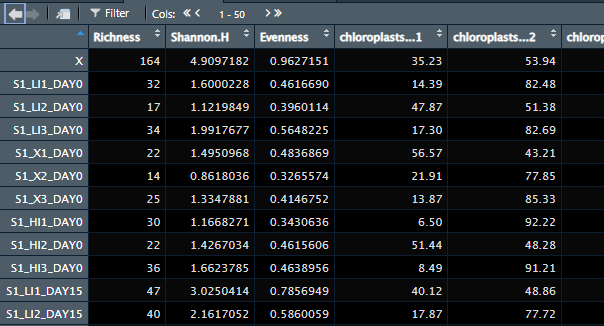
\includegraphics{./images/results_diathor.png}
\caption{Figura 7.1. Primeras filas y columnas de la tabla de resultados de DiaThor}
\end{figure}

Veremos que cada muestra (fila) tiene sus valores de diversidad (\emph{Richness, Shannon.H, Evenness}), porcentajes de número y forma de cloroplastos (\emph{chorloplasts, shape.chloroplasts}), porcentaje de diatomeas de cada clase de tamaño (\emph{size.class}), porcentaje de diatomeas de cada gremio ecológico (\emph{guilds),} los valores de cada índice de Van Dam (\emph{VD.Salinity, VD.NHet, VD.Oxygen, VD.Saprobity, VD.Aero, VD.Trophic}) y luego todos los índices bióticos.

Luego de cada uno de los índices, se encuentra una columna que indica cuántas especies \textbf{no fueron} determinadas en cada muestra (terminan en ``.\emph{Indet}'') y cuantas fueron usadas (terminan en ``.\emph{Taxa.Used}'').

\hypertarget{la-sintonuxeda-fina-veamos-las-salidas}{%
\subsubsection{\texorpdfstring{\textbf{La sintonía fina: veamos las salidas!}}{La sintonía fina: veamos las salidas!}}\label{la-sintonuxeda-fina-veamos-las-salidas}}

Una vez que el paquete termine el análisis, vaya a la carpeta adonde se guardaron los resultados. Se encontrará con varios archivos:

\begin{itemize}
\item
  \textbf{\emph{Diato\_results - Results.csv}}: Este archivo contiene la tabla principal de resultados, con cada muestra (fila) y sus valores de los diversos índices que si se pudieron calcular (columnas).
\item
  \textbf{\emph{Plots.pdf}}: Se incluyen los gráficos de cada uno de los índices bióticos calculados (eje X) en cada uno de las muestras analizadas (eje Y) para poder visualizarlo. Son realizados con los mismos datos que se encuentran en la tabla de resultados.
\item
  \textbf{\emph{Taxa excluded}} y \textbf{\emph{Taxa included:}} Es MUY importante que se revisen estos dos archivos. En estos archivos veremos que taxa de nuestra lista de especies original fueron \textbf{incluídos} o \textbf{excluídos} en el cálculo de cada uno de los índices. También nos ayudará a reconocer potenciales errores de tipeo o de nombramiento de especies.

  \textbf{\emph{VanDam Taxa used.txt:}} En particular, los valores ecológicos de Van Dam son separados en un archivo de texto al resto de los resultados, porque suelen ser muy amplios. Aquí se indica en cada una de nuestras muestras los taxones que fueron incluídos en el cálculo de cada una de las tolerancias (\emph{salinidad, N-heterotrofía, requisitos de oxígeno, saprobiedad, humedad, estado trófico}).
\end{itemize}

\textbf{Es muy importante} que antes de reportar los resultados del análisis, se revisen cuidadosamente las salidas del paquete. Nos pueden indicar que hay especies con el nombre mal escrito, o que para el cálculo de algún índice en particular se utilizó poca cantidad de especies presentes, cuestionando así la precisión del mismo.

\hypertarget{algunas-aclaraciones-relevantes}{%
\subsubsection{\texorpdfstring{\textbf{Algunas aclaraciones relevantes:}}{Algunas aclaraciones relevantes:}}\label{algunas-aclaraciones-relevantes}}

\begin{itemize}
\item
  Sobre el reconocimiento de los nombres de las especies:

  \begin{itemize}
  \item
    DiaThor realiza \textbf{dos búsquedas} automáticamente de cada especie en nuestro archivo.

    \begin{itemize}
    \item
      Primero realiza una \textbf{búsqueda exacta} de cada especie comparandola contra todas las especies utilizadas en todos los índices bióticos y ecológicos.
    \item
      Aquellas especies que no son encontradas por este medio, las separa y las vuelve a buscar automáticamente por una \textbf{búsqueda heurística}, para tratar de contemplar aquellos errores en la escritura de los nombres (Quien no escribió incorrectamente `\emph{Nitzschia fasciculata}' alguna vez, que tire la primer piedra!).\\
      \strut \\
      Este tipo de búsqueda permite que haya un número determinado de caracteres distintos entre dos palabras para considerarlas iguales. Por defecto, este valor en las funciones de \emph{diaThor} es igual a 2. Por ejemplo, la búsqueda heurística encontraría a la especie `\emph{Nitzschia fasciculata}' aunque la hubieramos escrito como `\emph{Nitzschia fasiculata}', porque hay sólo 1 caracter distinto. Este valor de distancia se puede cambiar con el parámetro \texttt{maxDistTaxa}.

      \textbf{¡Cuidado!} Mientras más alto el valor de este parámetro, más chances de encontrar la especie que buscamos, pero más posibilidad de que confunda nuestra especie con otra de nombre similar, y se incrementa notablemente el tiempo que tarda en buscarlas.
    \end{itemize}
  \item
    Las especies que tienen \textbf{categorías subespecíficas} (variedades y/o formas) se deben indicar con ``var.'' y ``fo.''.

    \begin{itemize}
    \tightlist
    \item
      Ejemplo: \emph{Achnanthes exigua} var\emph{. exigua}'' o ``\emph{Gomphonema parvulum} var. \emph{parvulum} fo. \emph{parvulum}''. El texto no busca formatos, no es necesario poner las especies en itálicas o subrayadas.\\
      El paquete va a tratar de buscarlas de cualquier manera aunque no contengan estos acrónimos, pero las búsquedas son más precisas y rápidas cuando estan nombradas así.
    \end{itemize}
  \end{itemize}

  \hypertarget{preguntas-frecuentes}{%
  \subsubsection{Preguntas frecuentes}\label{preguntas-frecuentes}}
\item
  \emph{¿Hay problemas encontrando el archivo de entrada CSV?}

  La consola nos indica este error:

  \texttt{*cannot\ open\ file\ \textquotesingle{}nuestro\_archivo.csv\textquotesingle{}:\ No\ such\ file\ or\ directory}

  Si corremos la función \texttt{diaThorAll()} directamente, sin agregar argumentos o parámetros, \textbf{un cuadro de diálogo} nos pedirá que seleccionemos el archivo con nuestros datos.
\end{itemize}

\begin{Shaded}
\begin{Highlighting}[]
\NormalTok{resultados }\OtherTok{\textless{}{-}} \FunctionTok{diaThorAll}\NormalTok{() }\CommentTok{\#sin argumentos}
\end{Highlighting}
\end{Shaded}

\begin{itemize}
\tightlist
\item
  \emph{¿Nuestros datos están en abundancia relativa?}\\
  Hay que indicarselo, cambiando el argumento \texttt{isRelAb} a \texttt{TRUE}.
\end{itemize}

\begin{Shaded}
\begin{Highlighting}[]
\NormalTok{resultados }\OtherTok{\textless{}{-}} \FunctionTok{diaThorAll}\NormalTok{(}\AttributeTok{isRelAb=}\ConstantTok{TRUE}\NormalTok{)}
\end{Highlighting}
\end{Shaded}

\begin{itemize}
\tightlist
\item
  \emph{¿No encuentra las especies, y quiero hacer una búsqueda heurística más amplia?}\\
  Cambiemos el argumento \texttt{maxDistTaxa}.
\end{itemize}

\begin{Shaded}
\begin{Highlighting}[]
\NormalTok{resultados }\OtherTok{\textless{}{-}} \FunctionTok{diaThorAll}\NormalTok{(}\AttributeTok{maxDistTaxa=}\DecValTok{4}\NormalTok{) }\CommentTok{\#Ahora buscará nombres de taxa en las bases de datos internas con hasta cuatro caracteres de diferencia al ingresado en nuestro CSV.}
\end{Highlighting}
\end{Shaded}

\begin{itemize}
\tightlist
\item
  \emph{¿Y si quiero sólo calcular un índice, en vez de todo? Así es más rápido.}\\
  Podemos usar funciones para cada índice biótico o ecológico.
\end{itemize}

\begin{Shaded}
\begin{Highlighting}[]
\CommentTok{\#Primero, cargamos nuestros datos, como siempre}
\NormalTok{base }\OtherTok{\textless{}{-}} \FunctionTok{read.csv}\NormalTok{(}\StringTok{"sampleData\_diaThor.csv"}\NormalTok{) }\CommentTok{\#Corroborar que el nombre del archivo coincida con el que vamos a utilizar, y que se encuentre en la carpeta de nuestro proyecto}

\CommentTok{\#Luego, necesitamos que diaThor reconozca las especies por su nombre. Para esto existe la función diat\_loadData()}
\CommentTok{\#A esta función se le pueden pasar los mismos argumentos que a diaThorAll(). Es decir, podemos restringir la distancia heurística con \textquotesingle{}maxDistTaxa\textquotesingle{}, o indicar si los datos están expresados en abundancia relativa con \textquotesingle{}isRelAb\textquotesingle{}}

\NormalTok{resultados }\OtherTok{\textless{}{-}} \FunctionTok{diat\_loadData}\NormalTok{(base, }\AttributeTok{isRelAb=}\ConstantTok{TRUE}\NormalTok{, }\AttributeTok{maxDistTaxa =} \DecValTok{2}\NormalTok{) }\CommentTok{\#Ejemplo usando abundancias relativas y la distancia heurística por defecto = 2}
\CommentTok{\#Deberemos indicar una carpeta para los resultados, en el cuadro de diálogo }

\CommentTok{\#Y luego, por ejemplo, podemos calcular sólo el índice IDP}

\NormalTok{resultadosIDP }\OtherTok{\textless{}{-}} \FunctionTok{diat\_idp}\NormalTok{(resultados) }\CommentTok{\#Grabamos los resultados en el objeto resultados IDP}

\CommentTok{\#o el índice IPS}

\NormalTok{resultadosIPS }\OtherTok{\textless{}{-}} \FunctionTok{diat\_ips}\NormalTok{(resultados) }\CommentTok{\#Grabamos los resultados en el objeto resultados IPS}

\CommentTok{\#Hay funciones separadas para todos los índices del paquete; en la documentación se indican cuales, y se van agregando con las distintas actualizaciones.}
\end{Highlighting}
\end{Shaded}

\hypertarget{shiny}{%
\subsubsection{Shiny!}\label{shiny}}

Hay una versión online para utilizar el paquete \texttt{diaThor} a través de un entorno Shiny, en:

\url{https://limnolab.shinyapps.io/diathor-shiny/}

\hypertarget{fuentes-de-informaciuxf3n-ecoluxf3gica-de-las-especies}{%
\subsection{Fuentes de información ecológica de las especies}\label{fuentes-de-informaciuxf3n-ecoluxf3gica-de-las-especies}}

La información morfológica se busca en la base de datos del proyecto `Diat.Barcode':

\begin{itemize}
\tightlist
\item
  Rimet F., Gusev E., Kahlert M., Kelly M., Kulikovskiy M., Maltsev Y., Mann D., Pfannkuchen M., Trobajo R., Vasselon V., Zimmermann J., Bouchez A., 2019. Diat.barcode, an open-access curated barcode library for diatoms. Scientific Reports. \url{https://www.nature.com/articles/s41598-019-51500-6}
\end{itemize}

La clasificación de las especies por su clase de tamaño se obtiene de:

\begin{itemize}
\tightlist
\item
  Rimet F. \& Bouchez A., 2012. Life-forms, cell-sizes and ecological guilds of diatoms in European rivers. Knowledge and management of aquatic ecosystems, 406: 1-14. \url{https://www.kmae-journal.org/articles/kmae/abs/2012/03/kmae120025/kmae120025.html}
\end{itemize}

La clasificación de las especies en gremios ecológicos se obtiene de:

\begin{itemize}
\tightlist
\item
  Rimet F. \& Bouchez A., 2012. Life-forms, cell-sizes and ecological guilds of diatoms in European rivers. Knowledge and management of aquatic ecosystems, 406: 1-14. \url{https://www.kmae-journal.org/articles/kmae/abs/2012/03/kmae120025/kmae120025.html}
\end{itemize}

La clasificación combinada de gremios y clases de tamaño (más nueva) se obtiene de:

\begin{itemize}
\tightlist
\item
  B-Béres, V., Török, P., Kókai, Z., Lukács, Á., Enikő, T., Tóthmérész, B., \& Bácsi, I. (2017). Ecological background of diatom functional groups: Comparability of classification systems. Ecological Indicators, 82, 183-188. \url{https://www.sciencedirect.com/science/article/abs/pii/S1470160X1730420X}
\end{itemize}

Preferencias ecológicas para la clasificación de Van Dam se obtienen de:

\begin{itemize}
\tightlist
\item
  Van Dam, H., Mertens, A., \& Sinkeldam, J. (1994). A coded checklist and ecological indicator values of freshwater diatoms from the Netherlands. Netherland Journal of Aquatic Ecology, 28(1), 117-133.
\end{itemize}

Los índices de diversidad (Shannon H') se calcula usando internamente el paquete \emph{vegan} \citep{vegan}:

\begin{itemize}
\tightlist
\item
  Shannon, C. E., and Weaver, W. (1949). `The Mathematical Theory of Communication.' (University of Illinios Press: Urbana, IL, USA.)
\end{itemize}

Los valores de tolerancia y valencia de cada especie para cada índice biótico se obtiene de sus fuentes publicadas originales:

\begin{itemize}
\item
  \textbf{IPS}: Coste, M. (1982). Étude des méthodes biologiques d'appréciation quantitative de la qualité des eaux. Rapport Cemagref QE Lyon-AF Bassin Rhône Méditerranée Corse.
\item
  \textbf{TDI}: Kelly, M. G., \& Whitton, B. A. (1995). The trophic diatom index: a new index for monitoring eutrophication in rivers. Journal of Applied Phycology, 7(4), 433-444.
\item
  \textbf{IDP}: Gómez, N., \& Licursi, M. (2001). The Pampean Diatom Index (IDP) for assessment of rivers and streams in Argentina. Aquatic Ecology, 35(2), 173-181.
\item
  \textbf{DES}: Descy, J. P. 1979. A new approach to water quality estimation using diatom. Beih. Nov Hedw. 64:305-323
\item
  \textbf{EPID}: Dell'Uomo, A. (1996). Assessment of water quality of an Apennine river as a pilot study for diatom-based monitoring of Italian watercourses. Use of algae for monitoring rivers, 65-72.
\item
  \textbf{IDAP}: Prygiel, J., \& Coste, M. (1993). The assessment of water quality in the Artois-Picardie water basin (France) by the use of diatom indices. Hydrobiologia, 269(1), 343-349.
\item
  \textbf{ID-CH}: Hürlimann J., Niederhauser P. 2007: Méthodes d'analyse et d'appréciation des cours d'eau. Diatomées Niveau R (région). État de l'environnement n° 0740. Office fédéral de l'environnement, Berne. 132 p
\item
  \textbf{ILM}: Leclercq, L., \& Maquet, B. (1987). Deux nouveaux indices diatomique et de qualité chimique des eaux courantes. Comparaison avec différents indices existants. Cahier de Biology Marine, 28, 303-310.
\item
  \textbf{LOBO}:

  \begin{itemize}
  \item
    Lobo, E. A., Callegaro, V. L. M., \& Bender, E. P. (2002). Utilização de algas diatomáceas epilíticas como indicadoras da qualidade da água em rios e arroios da Região Hidrográfica do Guaíba, RS, Brasil. Edunisc.
  \item
    Lobo, E. A., Bes, D., Tudesque, L., \& Ector, L. (2004). Water quality assessment of the Pardinho River, RS, Brazil, using epilithic diatom assemblages and faecal coliforms as biological indicators. Vie et Milieu, 54(2-3), 115-126.
  \end{itemize}
\item
  \textbf{SLA}: Sládeček, V. (1986). Diatoms as indicators of organic pollution. Acta hydrochimica et hydrobiologica, 14(5), 555-566.
\item
  \textbf{SPEAR(herbicides)}: Wood, R. J., Mitrovic, S. M., Lim, R. P., Warne, M. S. J., Dunlop, J., \& Kefford, B. J. (2019). Benthic diatoms as indicators of herbicide toxicity in rivers--A new SPEcies At Risk (SPEARherbicides) index. Ecological Indicators, 99, 203-213.
\item
  \textbf{PBIDW}: Castro-Roa, D., \& Pinilla-Agudelo, G. (2014). Periphytic diatom index for assessing the ecological quality of the Colombian Andean urban wetlands of Bogotá. Limnetica, 33(2), 297-312.
\item
  \textbf{DISP}: Stenger-Kovács, C., Körmendi, K., Lengyel, E., Abonyi, A., Hajnal, É., Szabó, B., Buczkó, K. \& Padisák, J. (2018). Expanding the trait-based concept of benthic diatoms: Development of trait-and species-based indices for conductivity as the master variable of ecological status in continental saline lakes. Ecological Indicators, 95, 63-74.
\end{itemize}

\begin{center}\rule{0.5\linewidth}{0.5pt}\end{center}

\hypertarget{paquete-optimos.prime}{%
\section{\texorpdfstring{Paquete \emph{optimos.prime}}{Paquete optimos.prime}}\label{paquete-optimos.prime}}

\emph{Autores: Belén Sathicq, María Mercedes Nicolosi Gelis, Joaquín Cochero}

\hypertarget{quuxe9-hace-1}{%
\subsection{¿Qué hace?}\label{quuxe9-hace-1}}

El paquete calcula los valores \textbf{óptimos} y \textbf{rangos de tolerancia ecológicos} de los taxones a las variables ambientales que proveamos.

\hypertarget{cuxf3mo-lo-hace}{%
\subsection{¿Cómo lo hace?}\label{cuxf3mo-lo-hace}}

El enfoque más común utilizado para el cálculo de los óptimos y los rangos de tolerancia ecológicos es calcular la \textbf{media ponderada} (Birks et al.~1990; Potapova y Charles, 2003).

La \textbf{media ponderada} \(u_{k}\) de las estimaciones de los óptimos de las especies se calcula como:

\[
u_{k} =\sum_{i=1}^{n} y_{ik}x_{i}/\sum_{i=1}^{n}y_{ik}
\]

y la \textbf{tolerancia}, o desviación estándar ponderada \(t_{k}\), se calcula como:

\[
t_{k} = \sqrt{\frac{\sum_{i=1}^{n} y_{ik} (x_{i} - u_{k})^2}{\sum_{i=1}^{n} y_{ik}}}
\]

adonde \(y_{ik}\) es la abundancia relativa de la especie \(k\) en la muestra \(i\); \(x_{i}\) es el valor \emph{log10} del parámetro ambiental en la muestra \(i\); y \(n\) es el número total de muestras del conjunto de datos.

\hypertarget{manos-a-la-obra-2}{%
\subsection{¡Manos a la obra!}\label{manos-a-la-obra-2}}

Como ejemplo, vamos a utilizar parte del set de datos de la tesis doctoral ``\emph{Empleo de descriptores fitoplanctonicos como biomonitores en la evaluacion de la calidad del agua en la costa del rıo de la Plata (Franja Costera Sur)}'' de M.B. Sathicq (2017) \citep{sathicq2017}, pública en el \href{http://sedici.unlp.edu.ar/handle/10915/58915}{repositorio SEDICI de la UNLP}.

\hypertarget{descargar-los-datos-1}{%
\subsubsection{\texorpdfstring{\textbf{Descargar los datos}}{Descargar los datos}}\label{descargar-los-datos-1}}

Descargaremos dos sets de datos desde el repositorio del curso, y los debemos guardar en el Directorio de Trabajo del Proyecto que creamos para esta Unidad (ver cómo hacerlo en la Unidad \ref{intro}).

Descargar el set de datos ambiental desde aquí: \url{https://github.com/Limno-con-R/CILCAL2023/blob/main/datasets/environmental_data_OptimosPrime.csv}

Descargar el set de dato de especies por muestras desde aquí: \url{https://github.com/Limno-con-R/CILCAL2023/blob/main/datasets/species_data_OptimosPrime.csv}\\

\hypertarget{instalar-el-paquete-1}{%
\subsubsection{Instalar el paquete}\label{instalar-el-paquete-1}}

Instalaremos el paquete \emph{optimos.prime} \citep{sathicq2020} como se indica en la Unidad \ref{intro} y los cargaremos a nuestro espacio de trabajo actual:

\begin{Shaded}
\begin{Highlighting}[]
\FunctionTok{library}\NormalTok{(optimos.prime)}
\end{Highlighting}
\end{Shaded}

\hypertarget{cargar-y-previsualizar-nuestro-archivo-de-datos-1}{%
\subsubsection{Cargar y previsualizar nuestro archivo de datos}\label{cargar-y-previsualizar-nuestro-archivo-de-datos-1}}

Debemos cargar dos sets de datos. El primero contiene la información de las variables ambientales en cada sitio o muestra (``\emph{environmental\_data\_OptimosPrime}''). El segundo contiene la información de abundancia relativa de los taxa en cada sitio o muestra (``\emph{species\_data\_OptimosPrime}'').

\begin{Shaded}
\begin{Highlighting}[]
\NormalTok{env\_data }\OtherTok{\textless{}{-}} \FunctionTok{read.csv}\NormalTok{(}\StringTok{"environmental\_data\_OptimosPrime.csv"}\NormalTok{) }\CommentTok{\#Corroborar que el nombre del archivo coincida con el que vamos a utilizar, y que se encuentre en la carpeta de nuestro proyecto}

\NormalTok{species\_data }\OtherTok{\textless{}{-}} \FunctionTok{read.csv}\NormalTok{(}\StringTok{"species\_data\_OptimosPrime.csv"}\NormalTok{) }\CommentTok{\#Corroborar que el nombre del archivo coincida con el que vamos a utilizar, y que se encuentre en la carpeta de nuestro proyecto}

\CommentTok{\#Alternativamente, para seleccionar un archivo con un cuadro de diálogo, se puede usar la función \textasciigrave{}file.choose()\textasciigrave{}, así:}

\NormalTok{env\_data }\OtherTok{\textless{}{-}} \FunctionTok{read.csv}\NormalTok{(}\FunctionTok{file.choose}\NormalTok{()) }\CommentTok{\#y seleccionar el CSV con los datos ambientales}
\NormalTok{species\_data }\OtherTok{\textless{}{-}} \FunctionTok{read.csv}\NormalTok{(}\FunctionTok{file.choose}\NormalTok{()) }\CommentTok{\#y seleccionar el CSV con los datos de abundancia de especies}

\CommentTok{\#Cualquiera de estas dos opciones cargará nuestros datos a los objetos "env\_data" y "species\_data"}
\end{Highlighting}
\end{Shaded}

Veamos brevemente cómo está organizada la información de nuestras especies:

\begin{Shaded}
\begin{Highlighting}[]
\FunctionTok{str}\NormalTok{(env\_data)}
\end{Highlighting}
\end{Shaded}

\texttt{env\_data} es un objeto \texttt{data.frame} con 11 \texttt{obs.} o filas (\emph{parámetros ambientales}) y 51 \texttt{variables} o columnas (\emph{sitios muestreados, o muestras}).

\begin{Shaded}
\begin{Highlighting}[]
\FunctionTok{str}\NormalTok{(species\_data)}
\end{Highlighting}
\end{Shaded}

\texttt{species\_data} es un objeto \texttt{data.frame} con 57 \texttt{obs.} o filas (\emph{especies}) y 51 \texttt{variables} o columnas (\emph{sitios muestreados, o muestras}).

\textbf{¡Es importante que la cantidad de variables o columnas (\emph{sitios muestreados, o muestras}) sea igual en ambos sets de datos!}

\hypertarget{a-la-magia-1}{%
\subsubsection{\texorpdfstring{\textbf{¡A la magia!}}{¡A la magia!}}\label{a-la-magia-1}}

Vamos a ejecutar la función \texttt{op\_calculate()} , que se encargará de realizar los análisis de óptimos ecológicos y rangos de tolerancia de los taxones que ingresamos en \texttt{species\_data} a las variables ambientales que ingresamos en \texttt{env\_data} . Y dispondremos de los resultados en un único objeto de tipo \texttt{data.frame}, que aquí lo llamaremos \texttt{resultados}.

\begin{Shaded}
\begin{Highlighting}[]
\NormalTok{resultados }\OtherTok{\textless{}{-}} \FunctionTok{op\_calculate}\NormalTok{(env\_data, species\_data)}
\end{Highlighting}
\end{Shaded}

Cuando terminen los cálculos, en la consola nos indicará que ya podemos ver los resultados.

\texttt{{[}1{]}\ "Optimum\ values\ and\ tolerance\ range\ calculated\ and\ placed\ in\ the\ final\ data\ frame"}

\texttt{{[}1{]}\ "Use\ View()\ to\ view\ data\ frame\ with\ results"}

\begin{Shaded}
\begin{Highlighting}[]
\FunctionTok{View}\NormalTok{(resultados)}
\end{Highlighting}
\end{Shaded}

\hypertarget{los-resultados-1}{%
\subsubsection{Los resultados}\label{los-resultados-1}}

Si todo ha salido bien, debemos ver que el objeto \texttt{resultados} es una nueva matriz de 57 \texttt{obs.} o filas (\emph{especies}) y ahora 34 \texttt{variables} o columnas (\emph{parámetros ambientales}). Es decir, por cada uno de los parámetros ambientales que ingresamos (eran 11), vamos a tener una columna con su valor de óptimo ecológico y otras dos columnas con su rango ecológico máximo y su ecológico rango mínimo (33 columnas). La primera columna contendrá los nombres de las especies.

Veamos por ejemplo las columnas 2, 3 y 4.

La \textbf{columna 2} (``\emph{Conductivity uS/cm}'') indica el valor óptimo de conductividad eléctrica para las especies, y el nombre con las unidades fueron ingresadas por el usuario en la matriz de datos ambientales.

La \textbf{columna 3} (``\emph{Conductivity uS/cm - HIGH}'') indica el rango de tolerancia máximo, y la \textbf{columna 4} (``\emph{Conductivity uS/cm - LOW}''), el rango de tolerancia mínimo.

Es importante entender que los valores obtenidos responden a los óptimos, máximos y mínimos de los taxones en base a los valores de los parámetros ambientales ingresamos. Si luego incorporamos nuevas muestras (por ejemplo en otros ambientes) y encontramos las mismas especies en otras condiciones ambientales, los óptimos y rangos de tolerancia de esas especies van a cambiar. Es por eso que se les llama \emph{rangos ecológicos.}

\hypertarget{graficar-e-interpretar-nuestros-resultados}{%
\subsubsection{Graficar e interpretar nuestros resultados}\label{graficar-e-interpretar-nuestros-resultados}}

El paquete \texttt{optimos.prime} nos puede generar gráficos de tipo caterpillar con nuestros resultados para cada variable ambiental, con la función \texttt{op\_plot()}. A esta función le tenemos que indicar la matriz de resultados de la función \texttt{op\_calculate()}, y le podemos indicar los argumentos \texttt{label}, para personalizar la etiqueta del gráfico, y/o el argumento \texttt{html}. Éste último indica si el gráfico producido se realizará en formato HTML, que permite interactuar con los datos usando el mouse, y es el valor predeterminado. Si \texttt{html=FALSE}, nuestro gráfico será una imagen plana.

\begin{figure}
\centering
\includegraphics{./images/plot_optimosPrime.png}
\caption{Figura 7.2. Óptimos ecológicos y rangos de variación para las especies de algas en referencia al pH.}
\end{figure}

En el gráfico, se verán las especies (\emph{en el eje Y}) y la variable ambiental elegida (pH, \emph{en el eje X}). Los puntos verdes indican el \textbf{valor óptimo de cada especie}, y los bigotes indican los \textbf{rangos de tolerancia} de cada especie a esa variable.

Aquellas especies con rangos de tolerancia más bajos (ejs. \emph{Actinastrum fluviale}, o \emph{Euglena} \emph{acus}), son consideradas especies `sensibles' a esa variable ambiental, y aquellas con grandes rangos de tolerancia (ejs. \emph{S.nanus} o \emph{Tetrastrum} \emph{glabrum}) son consideradas especies `tolerantes'. A su vez en este ejemplo, aquellas con valores óptimos más altos (más arriba en el gráfico) son consideradas mas alcalófilas y las que se encuentran más abajo en el gráfico son especies más acidófilas. Es importante revisar aquellas especies que tienen rangos de tolerancia muy bajos (ej. \emph{A. distans}), ya que puede ser el resultado de una baja cantidad de presencias de esa especie en las muestras.

\begin{Shaded}
\begin{Highlighting}[]
\FunctionTok{op\_plot}\NormalTok{(resultados)}

\CommentTok{\#En la consola nos preguntará que variable queremos graficar, y deberemos ingresar el número de la variable. Por ejemplo, para seleccionar el pH escribiriamos el número 2.}
\end{Highlighting}
\end{Shaded}

\hypertarget{algunas-aclaraciones-relevantes-1}{%
\subsubsection{\texorpdfstring{\textbf{Algunas aclaraciones relevantes:}}{Algunas aclaraciones relevantes:}}\label{algunas-aclaraciones-relevantes-1}}

\begin{itemize}
\tightlist
\item
  \emph{¿Nuestros datos no se encuentran en abundancia relativa?}\\
  Hay que indicarselo, cambiando el argumento \texttt{isRelAb} a \texttt{FALSE}.
\end{itemize}

\begin{Shaded}
\begin{Highlighting}[]
\NormalTok{resultados }\OtherTok{\textless{}{-}} \FunctionTok{op\_calculate}\NormalTok{(}\AttributeTok{isRelAb=}\ConstantTok{FALSE}\NormalTok{)}
\end{Highlighting}
\end{Shaded}

\begin{itemize}
\tightlist
\item
  \emph{¿Nuestros datos ya fueron convertidos a log10?}\\
  Hay que indicarselo, cambiando el argumento \texttt{islog10} a \texttt{TRUE}.
\end{itemize}

\begin{Shaded}
\begin{Highlighting}[]
\NormalTok{resultados }\OtherTok{\textless{}{-}} \FunctionTok{op\_calculate}\NormalTok{(}\AttributeTok{islog10=}\ConstantTok{TRUE}\NormalTok{)}
\end{Highlighting}
\end{Shaded}

\hypertarget{shiny-1}{%
\subsubsection{Shiny!}\label{shiny-1}}

Hay una versión online para utilizar el paquete \texttt{optimos.prime} a través de un entorno Shiny, en:\\
\url{https://limnolab.shinyapps.io/OptimosPrime-Shiny/}

  \bibliography{biblio.bib}

\end{document}
